%% Thesis Template of GZ.Univ
%%   for using revised CASthesis package with LaTeX2e
%%
%% Created by snda.liu <thinksheng@foxmail.com>
%%
%% $Id: template.tex,v 0.33 2017/07/14 16:23:46   $

%%%请使用pdflatex或pdftexify编译






\documentclass[pdftex,notypeinfo,twoside,openany,UTF8,fntef]{CASthesis}
%oneside单面打印,twoside双面打印;支持环保,选择双面打印!
%twoside,openany只是表示pdf按照双面打印准备,当你去复印社时,依然需要跟老板说明:“你需要双面打印”。

\graphicspath{{chapter/}{figures/}} % 设置图形文件的搜索路径

\CTEXsetup[format+={\flushleft}]{section} % 小节标题靠左对齐

\allowdisplaybreaks[4] %公式强制分页

\renewcommand{\baselinestretch}{1.5} %行间距,默认为1.3
\usepackage{setspace}
\usepackage{booktabs}
\usepackage{graphicx}
\usepackage{times}
\usepackage{mathptmx}
\usepackage{subcaption}
\usepackage[]{algorithm2e}
\usepackage{booktabs}
\usepackage{relsize}
\usepackage{colortbl}
\usepackage{enumerate}
\usepackage{amsmath}
\usepackage{tikz}
\usepackage{pgf}
\usepackage{pbox}
\usepackage{rotating}
\usepackage{multirow}
\usepackage{balance}
\usepackage{tablefootnote}
\usepackage{epstopdf, epsfig}
\usepackage{url}
\usepackage{cleveref}[2012/02/15]
\usepackage{arydshln}
\usepackage[super]{gbt7714}
\usepackage{geometry} %设置页边距
\geometry{left=2.54cm,right=2.54cm,top=3.17cm,bottom=3.17cm}

\setcounter{tocdepth}{2}%设定目录层级(通常取值0-2之间)

\theoremstyle{THrm}{
	\newtheorem{question}{Question}[section]
	\newtheorem{property}{性质}[section]
	\newtheorem{assumption}{假设}[section]
	\newtheorem{claim}[lemma]{断言}
	
}


\begin{document}


%%%%%%%%%%%%%%%%%%%%%%%%%%%%%%
%% 封面部分
%%%%%%%%%%%%%%%%%%%%%%%%%%%%%%

  % 中文封面内容
  \classification{TP309,TN918}%分类号
  \confidential{公开}%密级
  \serialnumber{2015010008}%论文编号
  \school{贵\ \ 州\ \ 大\ \ 学}
  \degree{2019届博士}
  \title{理性隐私保护模型及应用}
  \author{丁红发}
  \advisor{向淑文、彭长根}
  \xuekezhuanye{应用数学}
  \yanjiufangxiang{密码学与数据安全}
  \riqi{2019年12月}
  \didian{中国$\cdot$贵州$\cdot$贵阳}
%  请适当替换上述文字


 \oddyemei{\leftmark}
 \evenyemei{贵州大学博士学位论文}


  % 封面
  \maketitle
  \frontmatter%前序页码i ii iii iv
  % 目录
  \tableofcontents
  % 表格目录
 % \listoftables
  % 插图目录
 % \listoffigures
 \cleardoublepage


%%%%%%%%%%%%%%%%%%%%%%%%%%%%%%
%% 前言部分
%%%%%%%%%%%%%%%%%%%%%%%%%%%%%%


%%%%%%%%%%%%%%%%%%%%%%%%%%%%%%%%%%%%%%%%%%%%%%%%%%%%%%%%%%%%%%%%%%%%%%%%%%%%% 摘要


\begin{abstract}
信息化的快速发展和深度应用所引发的隐私安全挑战,成为了制约数据开放、共享、交换和应用的瓶颈,并引起了法律界和学术界的高度关注。从技术的角度,差分隐私保护算法作为一种重要的隐私保护技术,在面向多维及其复杂关联的数据隐私保护方面的研究还不够成熟。首先,由于数据类型混合、稀疏性、域值空间大等原因,差分隐私的多维数据处理面临隐私脆弱性、计算效率低等方面的挑战;其次,数据融合的关联性、背景知识攻击和策略型敌手攻击,数据的隐私性和可用性的矛盾成为了突出问题。针对上述问题,从博弈的角度探讨隐私与效用的均衡及优化,不失为一种较好的解决方案。本文重点围绕隐私与效用均衡这一核心问题,基于信息熵、优化理论和博弈均衡等相关理论和方法,以构建均衡、优化模型为主线,在隐私量化方法设计、隐私与效用博弈模型构建及均衡求解、优化模型建立及求解等方面,取得了一系列的成果,为从技术和管理相结合的视角解决隐私保护问题提供了借鉴。本文所取得的主要研究成果包括:

1. 提出了差分隐私的信息熵度量模型及方法。针对隐私量化问题,基于Shannon基本通信模型,结合差分隐私的随机扰动原理,给出了有噪声信道的差分隐私通信模型及其形式化描述;进一步通过定义差分隐私保护模型中的信息熵、条件熵、联合熵、互信息量以及条件互信息量等概念,设计了以信息熵为核心的隐私度量模型;针对多维属性及其关联问题,基于图模型和马尔可夫模型等提出了面向多关联属性的差分隐私信息熵度量模型及方法,并基于数据处理不等式和Fano 不等式给出了信息泄露量的上下界。理论分析与实验结果表明,所提出的量化模型和方法能够有效地实现差分隐私量化目标,为隐私泄露风险评估和隐私保护机制设计提供了基础支撑。

2. 提出了含背景知识攻击的差分隐私优化模型。在所建立的差分隐私通信模型的基础上,结合所提出的隐私度量模型与方法和损失压缩理论,建立含背景知识的敌手模型,以此为基础提出了含背景知识攻击的差分隐私通信模型;在基于条件互信息量设计的隐私率失真函数基础上,提出了含背景知识攻击的最优化模型;进一步针对所提出优化模型的求解问题,利用Blahut-Arimoto交替最小化方法设计和实现了权衡隐私与效用的迭代最小化算法,并给出了其计算复杂度分析。
理论分析和实验仿真结果表明,所提出的相关方法相对于对称信道隐私保护机制具有明显优势。

3. 提出了有序随机响应扰动方案(Orderly Randomized Response Perturbation,ORRP)。针对多维数据差分隐私保护所面临的隐私脆弱性和效率低问题,面向数据收集场景的隐私保护需求,提出了一种有序随机响应扰动方案,有效解决了现有隐私保护机制忽视数据分布的影响、处理域值空间大和数据稀疏导致计算效率低的问题。该方案以所提出的隐私度量模型为基础,通过对隐私保护与数据可用性之间矛盾的分析和量化,给出了满足数据质量约束下最小化隐私泄露的互信息优化模型的形式化描述,以此实现最优隐私机制的概率密度函数计算并实现随机扰动。同时,参考独立并联信道模型,将上述结果推广到了多维数据情形。最后,从隐私泄露、数据可用性质量、关联度损失等方面给予了理论分析和实验仿真。结果表明,所提出的ORRP方案在数据语义完整性、隐私性和数据可用质量等方面比现有的结果更具有优势。

4. 提出了隐私保护的攻防博弈(Privacy-Preserving Attack Defense,PPAD)模型。针对差分隐私系统中存在消息灵通的策略型敌手问题,围绕数据收集场景设计了差分隐私保护的选择策略,以此为基础提出了隐私保护的攻防博弈模型,并通过均衡求解实现了差分隐私保护中隐私与效用之间的平衡。该方案基于所建立的差分隐私基本通信模型,在分析隐私保护方和策略型敌手方各自目标的基础上,构建了隐私极小极大优化模型,给出了包含参与者集合、策略空间、收益函数等的隐私攻防博弈模型的形式化描述。论文巧妙地利用了隐私互信息量的内涵与外延,构造了隐私保护的效用函数,最终具体实现了一个两方零和对策博弈模型的构建。论文利用极小极大定理和凹凸博弈理论给出了该攻防博弈模型的均衡分析,并进一步基于最优策略响应设计了均衡求解的策略优化选择算法。理论分析与数值实验结果表明,所提出的模型及方法能有效解决等价隐私保护机制之间的比较问题,同时可用于隐私保护程度最差情况下的隐私泄露风险评估。





\keywords{隐私度量,差分隐私保护,率失真函数,博弈均衡,优化模型}
\end{abstract}


\begin{englishabstract}
The challenges of privacy and security caused by the rapid development of informatization and in-depth applications, have become a bottleneck restricting data opening, sharing, exchange, and application, and have attracted great attention from the legal and academic communities. From the perspective of technology, the differential privacy (DP) protection algorithm, as an important privacy protection technology, is not mature enough in the research of data privacy protection for multi-dimensional and complex associations. Firstly, due to the mixed data types, sparseness, and large domain value space etc, the multi-dimensional data processing of DP is faced with the challenges such as privacy vulnerability and low computational efficiency. Secondly, the relevance of data fusion, background knowledge attacks and strategic adversary attacks, and the contradiction between data privacy and usability have become prominent issues. For the problems mentioned above, it is a better solution to investigate the trade-off and optimization of privacy and utility from the perspective of the game theory. Thus, this article mainly focuses on the crucial problem of the trade-off between privacy and utility. Based on information entropy, optimization theory and game equilibrium and other related theories and methods, the equilibrium and optimization models are constructed as the main line of this research. A series of results have been achieved in designing of privacy quantification methods, constructing and solving game model between privacy and utility, optimization model establishment and solving, etc., which provide a reference for solving privacy protection issues from the perspective of combining technology and management. The major contributions can be summarized as follows.

1. The information entropy metric models and methods of DP are proposed. For the quantitative problem of privacy, the noisy DP communication model and formalization statement are defined based on the Shannon's fundamental communication model and the randomized perturbation principle of DP. Further, the notions of information entropy, conditional entropy, joint entropy, mutual information and conditional mutual information, etc., are defined under the differential privacy model, and then, the privacy metric models with information entropy as the core are designed. For the problem of multi-dimensional and correlated attributes, based on the graph and Markov model, etc., a privacy metric model and method for multi-dimensional and correlated attributes is proposed. Then, the upper and lower bounds of privacy leakage are quantified by using data processing inequality and Fano's inequality. Theoretic analysis and experimental results are demonstrating the proposed metric model and method can effectively achieve the goal of DP quantification, and further provide basic support for privacy leakage risk assessment and privacy protection mechanism design.


2. The differential privacy optimization model with background knowledge attacks is proposed. Based on the established fundamental communication model of the DP, lossy compression theory and the proposed privacy metric model, the adversary model which has relevant background knowledge is established, and further the DP communication model with background knowledge attacks is proposed. By using conditional mutual information measures privacy, this paper updates the form of the well-known rate distortion function, and proposes the differential privacy optimization model with background knowledge attacks. Further, the alternating minimization iteration algorithm solving the proposed optimization model is designed and implemented based on the Blahut-Arimoto alternating minimization method, and the computation complexity analysis is provided. Theoretic analysis and experimental results are demonstrating the proposed method have significant advantages in data quality and privacy leakage when compared with the existing symmetrical channel mechanism.


3. The orderly randomized response perturbation (ORRP) scheme is proposed. For the problem of low efficiency and privacy vulnerability when deal with multi-dimensional data using local differential privacy, and facing the privacy protection requirements of data collection scenarios, this paper proposes an orderly randomized response perturbation scheme. The proposed ORRP scheme effectively solves the impact of the existing privacy protection mechanisms ignoring data distribution, and the problem of low computing efficiency caused by the large processing domain value space and sparse data. To be specific, the proposed ORRP scheme based on the prior proposed privacy metric model. A mutual information optimization model subjects to a given data quality loss constraint to minimize privacy leakage, is proposed by analyzing and quantifying the requirements of privacy and data quality. Further, the probability density function (PDF) of the optimal privacy mechanism is computed by the means above, and it is used to achieve randomized perturbation. Meanwhile, referring to the independent parallel channel model, the above methods are extended to the case of multi-dimensional data. Finally, theoretical analysis and experimental simulations are given in terms of privacy leakage, data usability quality, and correlation loss. The results demonstrate that the proposed ORRP has more advantages than the existing methods in terms of data semantic integrity, privacy and data availability quality.


4. The privacy-preserving attack and defense (PPAD) game model is proposed. For the problem of informed and strategic adversary in the differential privacy system, the selection strategy of differential privacy protection is designed around the data collection scenarios. On the basis of the above, the PPAD game model is proposed, and the trade-off between privacy and utility in the protection of differential privacy is achieved by solving the equilibrium. The proposed scheme is based on the established differential privacy basic communication model. The privacy minimax optimization model is established by analyzing the privacy goals of defender and strategic attacker, and further the formalization statement of PPAD is provided, which includes players' sets, strategic spaces and payoff functions etc. This paper cleverly uses the connotation and extension of private mutual information to construct the utility function of privacy protection, and finally realized the construction of a two-person zero-sum (TPZS) game model. Then, this paper provides the game analysis by using von Neumann's minimax theorem and concave-convex game, and further designs a strategy optimization selection algorithm to calculate saddle point based on the optimal strategy response. Theoretic analysis and numeric simulation results show that the proposed model and method can effectively solve the problem of comparison between equivalent privacy mechanisms, and also can be used for privacy leakage risk assessment in the worst case of privacy protection.







\englishkeywords{Privacy metric, differential privacy protection, rate-distortion function, game equilibrium, optimization model
}
\end{englishabstract}


%%%%%%%%%%%%%%%%%%%%%%%%%%%%%%%%%%%%%%%%%%%%%%%%%%%%%%%%%%%%%%%%%%%%%%%%%%%%% 摘要结束



%%%%%%%%%%%%%%%%%%%%%%%%%%%%%%
%% 正文部分
%%%%%%%%%%%%%%%%%%%%%%%%%%%%%%
\mainmatter%正式页码1 2 3

%%%%%%%%%%%%%%%%%%%%%%%%%%%%%%%%%%%%%%%%%%%%%%%%%%%%%%%%%%%%%%%%%%%%%%%%%%%%% 第1章


\chapter{绪论}
\label{chap:intro}

\section{研究背景及意义}
互联网、移动互联网和物联网快速发展,以及5G技术的不断推进和商用推广,社交网络、位置服务、医疗健康、生物基因、工业控制等海量数据被主动或被动采集、传输、存储、流转、分析并应用。海量数据的产生和应用推动了云计算、大数据和边缘计算等新兴产业和技术的爆发式增长,并产生了智慧医疗、智慧交通、智慧政府、智慧城市等不同的应用,极大地丰富了人们的物质和精神生活。同样,数据海量化增长、网络跨域泛在、计算云端化、应用多样复杂化等新的变化为安全和隐私带来了巨大挑战,大量的病毒、漏洞、攻击和数据关联分析,致使隐私严重泄漏,引发了人们极大的担忧。表~\ref{tab:privacy_leakeges}展示了近年来主要的隐私泄露事件,充分表明了隐私泄露已经成为网络空间的重要威胁。在此背景下,深入的理解隐私并保护隐私变得尤为重要。

\begin{table}[htbp]
\caption{近年来主要隐私泄露事件简况}
\label{tab:privacy_leakeges}
\centering
\begin{tabular}{p{0.12\textwidth}p{0.22\textwidth}p{0.25\textwidth}p{0.25\textwidth}}%

	\toprule
	\textbf{时间}&\textbf{事件}&\textbf{影响}&\textbf{原因}\\
	\midrule
	2017年7月 & 韩国加密货币交易所客户数据泄露 & 3万个人用户数据被盗并遭受电话诈骗 & 黑客入侵攻击\\
	2017年10月 & 全球11个国家41个凯悦酒店数据泄露 & 数据量不详,涵盖信用卡姓名、卡号、到期日期、验证码等 & 通过恶意软件进行黑客入侵\\
	2017年10月 & 马来西亚超过总人口的手机用户信息泄露 &4620万人用户地址、身份证号、手机识别卡信息泄露 & 不详\\
	2017年10月 & 埃森哲服务器大量敏感信息泄露 & 19亿敏感的密码和解密密钥泄露 & 操作失误将数据放到未保护的云服务上\\
	2017年10月 & 南非史上最大规模数据泄露 & 3160万人个人资料被公之于众 & 数据在未保护的服务器上导致黑客窃取\\
	2018年3月 & Facebook用户数据泄露 & 5千万用户数据泄露,影响美国大选 & 越权采集并分析用户喜好、性格、行为特点、政治倾向\\
	2018年8月 & 华住集团数据泄露 & 5亿条、140G华住旗下酒店的用户数据泄露 & 不详\\
	2018年8月 & 谷歌采集设备、地图、搜索位置信息 & 全球超20亿用户数据被越权采集 & 谷歌公司故意采集\\
\bottomrule
\end{tabular}
\end{table}

由于90\%以上的数据被提供公共服务的政府、社会组织和企业所采集、存储,为了使数据发挥更大的价值,往往需要对包含大量隐私信息的数据进行共享、开放、交换和分析处理;同时很多信息服务也是基于个人隐私信息与服务质量的交换,如网站注册服务、公共WIFI接入、云存储、智能手机导航、信息搜索与广告推送、在线信用卡支付、RFID应用等。这些场景中由于法律法规要求和个人意愿,需要对隐私信息进行保护,同时服务提供方、数据利用方或恶意第三方希望获取更多的隐私敏感信息,以提供更好的服务、获取更大数据价值,得到更好的数据效用,两个目标同时存在且相互冲突,需要均衡解决。

关于隐私的研究,自2006年~$k$~匿名模型~\cite{sweeney2002k}被提出以后逐步变成系统化的研究,隐私研究发展为基于密码学的方案~\cite{nabeel2014privacy,huang2015review}和基于非密码学的方案~\cite{sweeney2002k,machanavajjhala2007l,li2007t,dwork2006differential,zhang2018privacy}两大类,这些方案被大规模应用于以数据为中心的开放、复杂、跨域场景中,如云存储、社交网络、基于位置服务、物联网、边缘计算、数据挖掘、机器学习、医疗健康等。众多应用场景中,隐私保护目标和数据利用目标天然矛盾,如何平衡二者的关系是核心问题之一。在这两类隐私研究中,基于密码学的方案通常利用可证明安全理论定义密码学意义上的隐私保护目标,设计对应的密码学方案,如同态加密、可搜索加密、属性密码方案等实现隐私保护目标~\cite{nabeel2014privacy,huang2015review}。基于非密码学的方案主要是定义了匿名性设计达到匿名化效果的算法来实现用户的身份匿名隐私保护~\cite{sweeney2002k,machanavajjhala2007l,li2007t};通过定义邻近数据集的查询结果不可区分性,设计加噪的方法达到这种不可区分性来实现属性值的隐私保护~\cite{dwork2006differential};通过定义数据动态隐私,设计自适应的风险的细粒度访问控制实现隐私数据不被非授权用户访问~\cite{zhang2018privacy}。其中,基于密码学的方案具有严格的理论方法支撑,能够达到预期的隐私保护目标,但是这些隐私定义是密码学意义上安全性定义,隐私保护方案设计也依赖公钥密码,其计算高度复杂导致效率低下,且难以采用折中的措施实现隐私保护效果和数据效用的平衡;基于非密码学的方案通过概率或信息论定义匿名性和不可区分性意义上的隐私,并设计泛化匿名或加噪的方式实现匿名或属性值隐私保护,效率高且有利于平衡隐私保护效果和数据效用。目前,以数据为中心的开放应用场景多样化,特别是数据开放共享应用中,大规模的个人隐私需要在保证数据可用的前提下得到实用性的隐私保护,研究基于非密码学的方案可以达到这一目标,平衡隐私保护与数据效用,具有重要的现实意义。

隐私领域的研究主要有三方面科学问题。\textbf{第一、隐私定义与度量}。如何恰当形式化的定义隐私、并对隐私进行量化。特别是隐私量化,既包括对特定数据集中隐私量的量化,又包括在某种隐私分析攻击模型下,个人隐私潜在泄露量、隐私分析攻击后隐私泄露量评估,还包括某一隐私保护模型对数据集隐私保护强度的量化。\textbf{第二、隐私分析与推断}。在某一场景下针对保护后的隐私信息数据集进行隐私分析与推断,如何最大程度的获取更多隐私信息。\textbf{第三、隐私保护}。如何对某一场景下的隐私数据集进行有效隐私保护,如何在保护隐私的同时平衡隐私保护效果和数据效用。深入研究科学问题一和科学问题二有助于对隐私的理解和认识,能够对隐私泄露的机理进行深入剖析,能够对设计更好的隐私保护方案提供科学理论依据和评价方法,研究科学问题三能够实现对数据隐私的预期性保护,如可量化的、动态性的及自适应的隐私保护,能够平衡隐私保护效果与数据效用间的关系。上述三个科学问题对基于非密码学的方案研究有重要的理论意义,能够有助于该领域完善其基础理论体系,可在保证其实用性基础上提高隐私定义形式化及度量、隐私泄露机理、隐私保护方案的科学性。

面对上述隐私领域的主要科学问题挑战,本文主要针对数据开放共享场景下的基于非密码学隐私研究领域,展开隐私度量、隐私分析、隐私保护,以及隐私保护与数据效用平衡方面研究,旨在能够深入探究隐私基础理论,提高对隐私泄露及隐私保护机理的理解,以提出能够动态、自适应地对包含大量隐私信息的数据集进行隐私保护,并实现隐私保护与数据效用间的平衡。
\section{研究现状}

本节围绕本文的研究内容,就相关研究领域的现状进行梳理和分析,包括隐私度量、隐私分析、隐私保护,以及隐私保护与数据效用间的平衡四个方面,以更加深入的理解本文研究的背景。

\subsection{隐私度量}
早期对隐私的认知是法理上的“隐私权”,在技术上被定义为匿名性(Anonymity),即在一个匿名集中元素不能被唯一标识的状态。在匿名通信系统中,匿名性最初被量化为匿名集阶的自然对数~$a=log_2(N)~$\cite{reiter1998crowds},并有信息熵、正规熵、条件熵等方法,详见2009年Edman和Yener的综述~\cite{edman2009anonymity},但这些方法并不适用数据共享和应用中的匿名性度量。2002年,Sweeney~\cite{sweeney2002k}将数据集中某一记录的匿名性量化为~$d=1/k$~,其中~$k$~是数据集中与该记录不可区分的记录数量;随后,该方法被扩展为~$l$~多样性匿名~\cite{machanavajjhala2007l}和~$t$~邻近匿名~\cite{li2007t}。针对数据集的匿名性定义被扩展到了基于位置服务~\cite{niu2014achieving}、社交网络~\cite{campan2008data}等应用场景,并用以不同形式的数据发布~\cite{wong2006anonymity,ying2009comparisons}。这些方法都是将匿名性量化为与匿名集大小相关的概率值,并不能对敌手去匿名化攻击获取的信息量进行量化,且无法根据敌手的背景知识进行动态量化。Li等~\cite{li2010closeness}在~$k$~匿名和~$l$~多样性匿名的基础上,根据数据集中敏感属性的分布,通过EMD(Earth Mover's Distance)计算敏感属性全局概率分布和任意等价类中该属性值概率分布的差异,提高了匿名性度量的灵活性。林欣等~\cite{lin2009lbs}发现位置~$k$~匿名算法匿名集大小无法在连续查询攻击下刻画匿名集中位置的匿名度,提出了匿名集查询结果信息熵的匿名度量化方法~$D(q)=2^{H(q)}$~;Xu和Cai~\cite{xu2007location}认为在连续查询的位置~$k$~匿名中,模糊区域中用户会约束后续查询模糊区域的位置,进而提出了一种基于模糊区域大小和区域内实体数量的熵度量方法;为了使匿名性的度量能根据背景知识动态更新,王彩梅等~\cite{wang2012location}针对Slient Cascade轨迹隐私保护将模糊区域前后用户假名间的联系性进行量化~$D(u_i)=H(u_i)/H_{max}(u_i)$~。基于匿名集的大小及其数据概率分布对匿名性的度量,不能达到数学上的严谨证明,2006年Dwork~\cite{dwork2006differential}定义了差分隐私的概念,并通过添加高斯或拉普拉斯噪音的方法保护隐私,应用控制噪音量的隐私预算~$\epsilon$~来量化隐私;2016年,Cuff与Yu~\cite{cuff2016differential}应用互信息给出了差分隐私算法对隐私保护的上界;随后,Wang等~\cite{wang2016relation}从信息论角度对差分隐私、可识别性与互信息间的关系进行了量化。为了提高差分隐私的适用性,~$(\epsilon,\delta)$~差分、本地差分~\cite{kairouz2014extremal}和Renyi差分~\cite{mironov2017renyi}的定义被相继提出,基于匿名和差分结合的新的隐私定义也被提出~\cite{holohan2017k},并应用Renyi熵等信息论工具对差分隐私能力进行了量化。身份隐私的另外一类是成员关系隐私(Membership Privacy),即某一实体是否属于特定数据集的关系。2013年,Li等~\cite{li2013membership}定义了积极成员隐私和消极成员隐私,并分析了成员关系隐私与差分隐私间的关系。

云数据共享、位置服务、社交网络等众多场景中,数据集中的个人身份信息是对外公开的,需要对数据某字段值、位置点、个人喜好、政治倾向等属性隐私进行量化和保护,主要还是通过取值范围、集合的阶、正确率、精准率、信息熵、互信息等方面进行量化~\cite{xiong2018research,wagner2018technical}。除了对隐私进行分类定义和量化之外,对隐私保护算法的能力与敌手模型隐私分析攻击强度也需要量化。2011年,Shokri等~\cite{shokri2011quantifying}将轨迹去匿名化、位置攻击、会面泄露攻击等形式化为概率推断,并应用推断得到条件概率来估计隐私分析结果,应用精准度、正确性、确定性三个指标来量化隐私信息,度量隐私保护算法的性能。2015年,Ma等~\cite{ma2015information}对时间序列型数据隐私进行量化,除了利用互信息、正规互信息和条件熵,还提出了离线条件熵,即某时间点相邻的数据点协助推断该时间点的条件熵来量化隐私。2018年,Zhao与Wanger~\cite{zhao2018evaluating}应用一致性指标对图结构匿名性、可去匿名化从成功率和信息泄漏量等方面进行量化。此外,俞艺涵等~\cite{yu2018shannon}利用信息熵和BP神经网络实现隐私数据分级分类,对数据集记录的隐私量采用两层信息熵加权的方式进行量化。

可见,隐私量化主要是根据隐私定义和隐私目标进行形式化的,通过不同形式的可量化指标进行度量,对隐私保护机制能力和隐私分析攻击模型能力的量化主要是通过隐私数据集中元素的前后变化量来度量。这两方面的度量还未形成统一的框架,尽管信息论等工具被广泛应用于隐私量化,还需要在基础框架上进行统一,为不同场景下隐私目标的设定、隐私的量化提供理论支持;同时,还需要对多样化的应用场景定义适应性的隐私,以应对隐私的动态性、多样性需求。

\subsection{隐私分析}
由于商业、政治利益,以及为了更好地理解隐私、量化隐私、保护隐私,隐私分析一直是研究热点,主要集中在去匿名化推断分析和属性值推断分析两方面。对基于位置服务中用户的位置信息进行直接~$k$~匿名保护的情况,林欣等提出了一种连续查询攻击~\cite{lin2009lbs},在不同~$k$~匿名保护算法下的位置查询中成功区别出位置发送者。2013年,Humbert等~\cite{humbert2013addressing}应用置信传播算法对亲属间的基因序列隐私进行了重构推断攻击分析,并应用信息熵、正确率来量化敌手获取的隐私量。2017年,Olteanu等~\cite{olteanu2017quantifying}利用置信传播算法对社交网络共现位置的隐私进行了推断攻击分析。2018年,Deznabi等~\cite{deznabi2018inference}利用亲属关系、基因组高阶关联、基因表现型等更多公开基因组数据,对亲属间的基因序列隐私进行了重构推断攻击分析,并量化了隐私攻击强度。Manousakas等~\cite{manousakas2018quantifying}利用图结构基于核的相似性构造了一个人类迁徙网络拓扑结构的去匿名化推断模型,成功识别出了手机移动网络中的个体身份。2019年,Cao等~\cite{cao2019quantifying}针对差分隐私保护的连续发布数据情形,建立了基于Markov关联的条件概率推断模型,从前向数据发布和后项数据发布分析了隐私泄露量的上界。关于成员关系隐私,2017年,Shokri等~\cite{shokri2017membership}通过对机器学习训练模型建立多个“
Shadow”模型,对输入数据进行多个模型训练,根据输出数据的分布差异判断目标数据记录是否属于某个训练集合。2018年,Rahman等~\cite{rahman2018membership}针对基于差分隐私的深度学习训练数据集,在不同的差分隐私预算下分析了图片分类学习模型的成员关系隐私。

可见,隐私分析主要是敌手利用获取的先验或后验知识,建立与隐私分析目标相关联的推断模型,通过置信度、置信传播、贝叶斯推断、Markov等方法建立概率推断优化模型,获取目标隐私信息。通过隐私分析,可以帮助人们更加深入的认识隐私,理解隐私泄露的深层原因,通过各种不同的隐私攻击敌手模型为更好地设计高效的隐私保护算法提供理论依据。在各类场景中隐私分析的敌手模型多样复杂,需要更加深入的研究数据共享应用领域的隐私分析方法。

\subsection{隐私保护}

针对数据集的隐私保护算法是在隐私定义和量化的基础上提出来的。针对匿名隐私,通过泛化的方法实现~$k$~匿名~\cite{sweeney2002k}(即数据集中任意记录都至少有~$k-1$~条数据与之无法区分)之后,因为不同的匿名性定义不适用所有的场景,不能抵抗链接攻击、动态攻击、背景知识攻击等,驱动了~$l$~多样性匿名~\cite{machanavajjhala2007l}、~$t$~邻近匿名~\cite{li2007t}算法的提出。如同隐私量化,实现这些不同匿名性的算法也被扩展到各个领域,如基于位置服务~\cite{niu2014achieving}、社交网络~\cite{campan2008data}、数据发布~\cite{wong2006anonymity,ying2009comparisons}。类似地,不同的差分隐私算法迅速发展,~$(\epsilon,\delta)$~差分、本地差分~\cite{kairouz2014extremal}、Renyi差分~\cite{mironov2017renyi}、分布式差分隐私~\cite{cheu2019distributed}等不同形式的算法被提出,并被应用于对抗生成网络~\cite{xu2019ganobfuscator},深度学习模型发布~\cite{yu2019differentially}和社交网络数据发布~\cite{wang2018real}等各类场景。

访问控制是一种有效的安全防护和隐私保护方法,也被广泛应用在各领域~\cite{li2017access}。2007年,Ni等~\cite{ni2007privacy}就扩展基于角色的访问控制使其适应隐私需求,还有更多面向隐私保护的访问控制模型被提出,如基于属性的隐私访问控制~\cite{edemacu2019privacy}。面向隐私保护的非密码学访问控制主要有基于信任~\cite{wang2019game}、基于风险~\cite{zhang2018privacy}、基于激励~\cite{liu2011risk}、基于目的访问控制~\cite{amini2019purpose}的方案。基于风险的访问控制具有较好的动态性和适应性,对系统设置依赖较为简单,在动态化细粒度的隐私保护需求方面受到了广泛关注。在Cheng等~\cite{cheng2007fuzzy}利用模糊逻辑提出多层安全的风险访问控制模型后,被迅速推广为标准草案~\cite{mcgraw2009risk}。2011年,Wang等~\cite{wang2011quantified}应用于保护医疗信息系统中病人隐私,随后有了更进一步的发展~\cite{zhang2018privacy,li2017access}。

可见,隐私保护研究的目标之一是设计更加严谨、有效、灵活的方案,包括基于非密码学和基于密码学的方案。鉴于本文主要关注前者,有关基于密码学的隐私保护方案可参阅黄刘生等~\cite{huang2015review}的综述。由于隐私保护的场景多样复杂,隐私需求动态变化,该领域需要更加丰富的研究,以支持当前以数据为中心的开放、动态应用场景隐私保护需求。

%更多基于非密码学隐私保护方案研究进展,可参阅文献~\cite{wang2014review}。
%鉴于基于密码学的隐私研究并非本文研究的聚焦点,尽管该领域亦有很多成果,本文也不再进行详述,可查阅基于属性密码~\cite{servos2017,edemacu2019privacy}、可搜索加密~\cite{boesch2014survey,poh2017searchable}、同态密码~\cite{acar2018survey}、安全多方计算~\cite{cramer2015secure,dugan2016survey}等领域的综述进一步了解。

\subsection{隐私与效用平衡}
除了要保护隐私,数据效用是数据发布或共享时考虑的重要因素,Li等~\cite{li2009tradeoff}较早考虑了数据发布的隐私与效用平衡问题,认为隐私泄露与效用获取不能直接对比,提出了一种基于投资组合风险与收益的隐私损失与数据效用对比方法。Sui与Boutilier~\cite{sui2011efficiency}在机制设计领域的第二价格拍卖协议和设施选址协议中,提出减少数据效用可以提高隐私保护效果。Guo与Chen~\cite{guo2012mining}通过挖掘Facebook的用户隐私设置和用户偏好,为用户个性化隐私设置和社交效用权衡提供支持。Sanker等~\cite{sankar2013utility}提出用条件熵和互信息对数据集共享时,在保证最低限度隐私保护来达到最大的数据效用关系进行权衡。Kalantari等~\cite{kalantari2018robust}对差分隐私保护从汉明失真的角度讨论了隐私与效用的权衡,并用互信息来量化隐私损失率。He与Li~\cite{he2019modeling}用概率模型基于因子图和DNA中基因型与表现型间的统计关系,提出了可优化隐私与效用的基因数据发布方案。这些方案都指出隐私与效用间存在权衡关系,但并未提出如何平衡该关系,如何达到隐私与效用间的平衡。博弈论作为解决合作与冲突的数学工具,在网络安全各领域都有广泛的应用~\cite{zhu2018game},天然适用于解决隐私领域的隐私保护与数据效用间的冲突与合作问题。Freudiger等~\cite{freudiger2009non}在2009年将~$n$~方完美信息博弈引入到位置隐私保护,分析了用户最大化其位置隐私的博弈均衡,并提出了基于贝叶斯纳什均衡的理性隐私保护方案;随后Santos等~\cite{santos2011collaborative}针对位置服务中多代理协作位置共享场景,应用纯策略博弈和流行病模型设计了阈值博弈策略,实现了多代理间的合作与非合作效用最大化。2014年,Wang和Zhang~\cite{wang2014stochastic}对智能手机上下文隐私感知的动态敌手模型,构建了~2~方零和博弈模型,并设计了动态优化的隐私防护措施。2017年,Shokri等~\cite{shokri2017privacy}进一步将博弈论应用于优化的轨迹隐私,实现隐私保护与位置数据效用的平衡。2019年Du等~\cite{du2018community}将社区结构的演化博弈应用于社交网络中用户社交关系与隐私保护行为建模,激励用户隐私保护行为动态演进。可见,博弈论对隐私保护与数据效用的平衡有重要的作用,访问控制作为隐私保护的重要工具~\cite{wang2011quantified,nabeel2014privacy,zhang2018privacy},也需要能够恰当的解决此问题。2014年,Hu等~\cite{hu2014game}面向社交网络协同数据共享,提出了一种基于多方访问控制的多方控制博弈模型,以平衡隐私控制者隐私设置与收益间的关系。2016年,Liu等~\cite{liu2016dynamic}将序贯博弈应用于多播蜂窝网络接入的混合访问控制中。Helil等~\cite{helil2017non}和Wang等~\cite{wang2019game}分别将非合作博弈应用于基于信任的访问控制模型中。2018年,Gao等~\cite{gao2018game}将信誉和重复公共物品博弈引入到云存储数据共享中,以解决服务提供者与数据访问者间的信用困境,提高存储率并降低参与者非诚实行为。

可见,尽管博弈论在平衡隐私保护与数据效用方面有诸多进展,但面向隐私保护的访问控制领域的进展还较少,无法有效解决数据共享过程中访问者访问隐私敏感数据时,系统隐私保护需求与用户数据效用需求间的平衡问题;此外,现有基于博弈的访问控制模型都假设参与者是完全理性的,总能采取最优策略,现实场景中参与者由于信息不完全等各类因素不能总是完全理性的,故难以适应真实场景,需要有更好的理性博弈模型,解决有限理性条件下访问隐私保护与数据效用间的平衡问题。

\section{关键研究问题}

本节围绕本文的研究内容,对相关的关键问题进行总结,为后文研究这些问题并提出相应的解决方案奠定基础。

\begin{enumerate}
	\item \textbf{隐私度量}。信息论已经成为隐私度量的重要工具,但其在匿名隐私、成员隐私和差分领域的应用仅利用了信息熵、互信息等概念~\cite{wagner2018technical},某一具体的度量方法往往仅能适用于一种具体的场景,尚未对隐私度量形成体系化的框架~\cite{shokri2011quantifying,manousakas2018quantifying};其次,对隐私保护机制和隐私分析敌手模型的度量也相对割裂,并未有统一的模型同时适用于两方面的度量;再次,当前的隐私定义和隐私量化都是静态隐私,由于隐私是一个随场景、时间和需求发生变化的感性概念,需要动态适应性的定义并量化隐私。
	
%	此外,现有的信息论度量方法大多基于Shannon信息论,仅有少量工作扩展应用了Renyi熵,由于Shannon信息论不能刻画偏好、结构等信息,对具有时间序列特征数据、复杂结构图数据的隐私量化有天然的不足,需要进一步扩展信息论工具,更加有效的量化复杂结构数据的隐私。
	
	\item \textbf{隐私分析}。隐私分析是建立在对隐私恰当定义并量化的基础上实施的,现有的隐私分析针对匿名性的分析,实现去匿名化的研究较多~\cite{lin2009lbs,manousakas2018quantifying},对实体属性的隐私分析还较少。大量数据在云服务等环境中存储、共享或应用,特别是隐私分析推断攻击对象相互关联、属性隐私相互关联,敌手获取的背景知识不明确且包含大量公开背景知识,隐私泄露机理变得难以梳理。现有的隐私分析主要围绕位置数据、社交网络数据等场景,需要以更强的背景知识假设,对新型数据如时间序列数据(如连续社交轨迹数据)、基因序列数据(如医疗基因组数据)等进行进一步分析,更加深入的理解隐私。
	
	\item  \textbf{隐私保护}。目前基于匿名、差分的隐私保护模型都是静态的、粗粒度的方案,且具体的方案仅适用于某一特定场景,难以适应数据存储、共享及应用过程中动态个性化的隐私保护,难以满足大规模数据及分布式大规模用户动态数据需求的隐私保护。细粒度的访问控制模型,特别是基于风险的访问控制模型具有更加适用于大规模数据的动态需求特征~\cite{li2017access},但在隐私风险定义和量化方面,在访问控制自适应性方面都需要进一步研究。
	
	\item \textbf{隐私保护与数据效用平衡}。数据效用成为隐私保护机制考量的重要因素,需要设计能够兼顾隐私保护需求和数据效用需求,且能平衡二者关系的隐私保护机制。在细粒度动态实现隐私保护的风险访问控制模型中,如何真实地刻画隐私保护和数据效用、如何设计恰当的博弈过程及求解其均衡,如何更加符合真实场景地描述隐私保护参与方的非完全理性行为,如何描述隐私保护与数据效用逐步达到均衡点的过程,都需要进一步研究。
\end{enumerate}

\section{研究内容和成果}

本文以国家自然科学基金项目《理性隐私计算及隐私风险可控技术研究》为支撑,主要聚焦在以信息论通信模型及其扩展工具研究隐私度量的基础性框架模型,能够对隐私定义、隐私分析攻击模型和隐私保护机制进行量化;以概率推断为工具建立序列型隐私数据的属性隐私分析敌手模型,并针对真实数据进行分析推断攻击,量化敌手隐私分析攻击强度;因风险访问控制模型为基础,定义并量化风险隐私,设计动态自适应访问控制模型;以博弈论为工具,刻画访问控制隐私保护机制参与者的隐私和数据效用需求的理性行为和有限理性行为,设计能动态平衡隐私保护和数据效用关系的理性风险访问控制隐私保护机制。本文的研究框架和内容如图~\ref{fig:chapter1-research-framework}所示,本文提出的成果在图~\ref{fig:chapter1-research-framework}中表为灰色,具体取得了如下成果。

\begin{figure}[htbp]
	\centering
	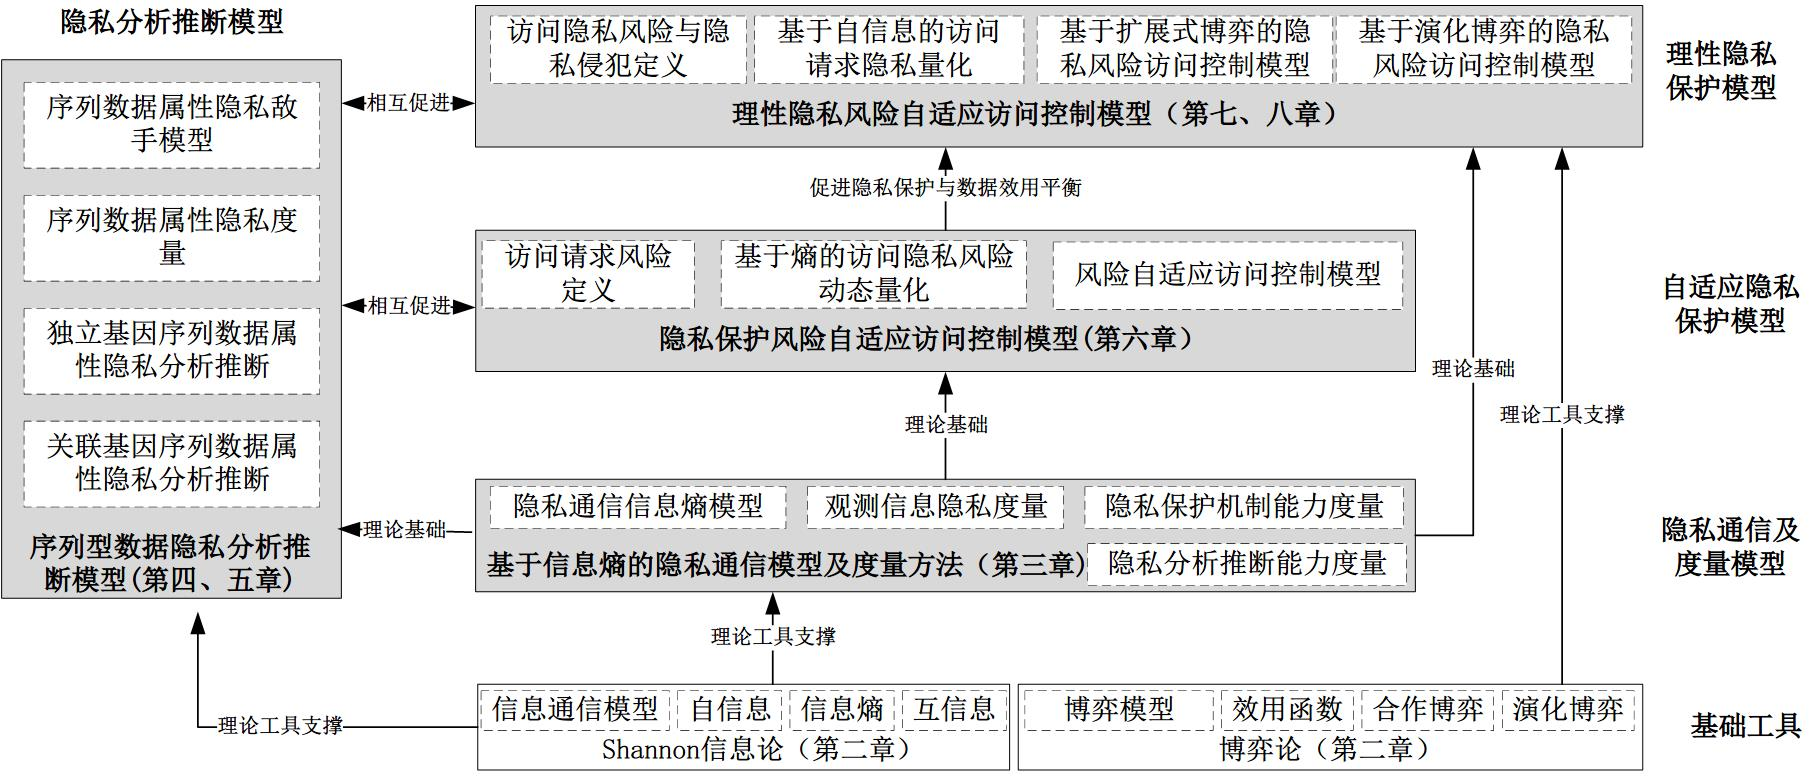
\includegraphics[width = 0.99\linewidth]{./figures/chapter1-research-framework.jpg}
	\caption{本文研究内容和框架结构}
	\label{fig:chapter1-research-framework}
\end{figure}
\subsection{基于信息熵的隐私通信模型及度量方法}
%\subsection{隐私通信模型及度量方法}
利用信息论的相关工具,如熵、互信息等来对匿名隐私、成员关系隐私和属性隐私进行形式化定义和度量的研究较多,但是大部分是集中在位置匿名、轨迹匿名、数据集匿名、数据集成员属性、训练集关系隐私、社交网络匿名和属性等方面的研究。在隐私量化方面,缺乏对隐私定义、隐私分析、隐私保护等统一的量化方法。

本文基于Shannon信息论的通信模型框架提出了几种隐私保护信息通信模型~\cite{peng2016privacy},对不含敌手的隐私保护、含敌手的隐私保护、多隐私保护源的隐私保护等不同情境提出了相应的模型进行建模,以满足对隐私度量、隐私保护机制效果度量和敌手隐私分析强度度量等需求。在所提出的度量模型中,将信息拥有者假设为发送方,隐私谋取者假设为接收方,隐私的泄露渠道假设为通信信道;基于该假设,分别引入信息熵、平均互信息量、条件熵及条件互信息等来分别描述隐私保护系统信息源的隐私度量、隐私泄露度量、含背景知识的隐私度量及泄露度量,形成了以信息论为核心的隐私度量方法体系;以此为基础,进一步提出了隐私保护方法的强度和敌手攻击强度的量化,为隐私泄露的量化提供了一种支撑,对整个隐私保护过程中的保护机制、敌手能力都提供了量化方法。%;最后,针对位置隐私保护的应用场景,通过所提出的隐私信息通信模型给出了具体的信息熵模型、以及隐私保护机制和攻击强度的度量及分析。

\subsection{独立序列型数据属性隐私推断模型}
近年来,由于数据种类繁多、数量庞大且应用需求多样化,越来越多的数据被以集中或分布式的形式共享、开放,造成了大量的隐私泄露,这些泄露又成为敌手进行隐私分析的背景知识,增加了数据共享的隐私泄露风险,对数据隐私泄露的潜在威胁量化,对数据隐私保护机制设计都提出了高的要求。特别是需要对隐私泄露的原理进行进一步研究,以帮助更好地度量隐私、理解隐私泄露机理,并设计更好的隐私保护方法。目前针对匿名方法的去匿名性分析研究较多,针对社交网络的用户偏好、个人信息等属性隐私的分析研究较多,但是对新型序列化数据的属性隐私,如时间序列的位置隐私、基因序列的基因座敏感值隐私较少,此类数据在很多共享应用场景(如疾病诊断、车联网导航)中需要非匿名化,需要对其敏感的属性隐私(特定基因座的基因型,特定行车位置)进行保护。

本文针对基因序列数据的属性隐私提出了一种基于概率推断的隐私分析模型。该模型通过对单条敏感数据记录属性值存在的相互关联关系进行分析,构建目标属性值推断的敌手模型。在提出的敌手模型基础上,分别提出了两种不同的基因序列属性隐私分析方法\cite{ding2010inferences}。第一种主要基于Monte Carlo-Markov抽样和隐Markov推断算法,建立了目标基因序列的“抽样解析”——“单倍体属性值概率推断”——“二倍体合成”三个步骤的属性隐私推断模型;第二种方法应用卷积神经网络构建概率推断算法,改进了单倍体属性值推断过程,实现了大规模序列型数据的属性推断目标。所提出的方法针对不存在亲属关系的群体基因序列数据共享场景,在本文第\ref{chap:entropy-metric-model}章提出的隐私度量模型基础上,定义了序列型数据属性隐私和量化方法,并应用于分析属性隐私泄露情况,通过量化隐私泄露量和敌手获取隐私量等信息,提高对序列型数据属性隐私的认识和理解。实验表明,本文提出的方法比现有基因序列属性隐私分析模型和算法更优,敌手对属性隐私的错误率、不确定度降低,敌手获得隐私信息量都比已有的工作更优。
\subsection{关联序列型数据属性隐私推断模型}

随着不同机构和个人更加容易获取基因组数据,且这些敏感数据被广泛地应用于医疗、保险、寻亲及社交等场景,对数据安全和隐私的担忧也在不断加剧。为了证实在序列型数据属性隐私方面,存在个人共享基因数据也会大量泄漏他人属性隐私的问题,为了进一步分析家族成员基因序列数据共享会造成他人基因序列属性隐私泄露的机理,需要对相互关联的基因序列型数据进行隐私分析。

本文利用因子图和置信传播算法针对亲属间的基因序列属性隐私建立分析推断敌手模型和分析算法。该模型考虑了单核苷酸多态性间高阶相关性,利用公开DNA参照数据集和全基因组关联研究(GWAS)目录数据,提高了推断攻击模型的属性隐私分析强度。该模型的敌手隐私分析强度通过本文所提出的隐私度量框架,对基因序列属性隐私进行了定义,并将隐私损失量作为评价指标进行了隐私分析强度量化。实验结果表明,所提出的攻击更适合于高密度基因组数据隐私推断,且具有较少的错误率、不确定性和更多隐私损失,显著提高了属性隐私的隐私分析推断能力。

\subsection{隐私保护风险自适应访问控制模型}
在以数据为中心的开放系统中,数据往往通过云服务或其他集中式的方式按需提供数据共享、开放、应用服务,这些需求多样复杂产生了复杂的隐私泄露风险和威胁,需要动态化、细粒度、适应性的方案对数据提供访问控制模式的隐私保护。但目前基于传统的强制访问控制、基于角色访问控制以及新型的基于属性访问控制,都不能很好的解决该问题。

本文针对云环境中共享、应用涉及隐私或敏感信息数据的场景研究面向隐私保护的访问控制模型\cite{ding2019risk}。在XACML上扩展提出了一种基于风险的自适应访问控制模型,以动态化地在访问控制过程中保护数据隐私,约束隐私侵犯行为,激励诚实访问行为。首先,根据风险访问控制场景的隐私保护需求提出了面向隐私保护的风险访问控制敌手模型;其次,该模型在标准的XACML框架进行了扩展,新增了策略风险评估、会话控制和风险消减服务三个组件,增强了策略执行、策略访问和策略信息组件。在新增的组件中,以Shannon信息熵作为工具,在第\ref{chap:entropy-metric-model}章提出的隐私度量模型基础上,提出了基于风险的隐私定义和量化方法,对用户的访问控制请求风险和用户自身的风险类型结合,提出了访问请求类型判别方法;通过风险隐私量化及基于信用卡模型的激励机制,实现访问行为风险阈值的动态调整,考虑了用户短期访问行为和长期访问行为的影响。对比和分析表明,所提出的模型和方法较现有的工作更加动态化,且实现了隐私保护,易用性更好。
\subsection{基于扩展式博弈的理性隐私风险访问控制模型}

基于风险访问控制模型可很好的解决以数据为中心的开放系统中自适应数据隐私保护。但强制访问控制、基于角色访问控制、基于属性访问控制和已有的基于风险访问控制等模型,在平衡隐私保护需求与数据效用需求冲突方面,仍存在问题,特别是过度授权导致隐私泄露或授权不足导致数据可用性不足的问题需要进一步解决。此外,还需要对基于风险访问模型中对隐私保护的能力和方法进一步提升。

针对上述需求和问题,本文在所提出的风险自适应访问控制模型的基础上,进一步运用Shannon自信息和博弈论,提出了基于风险适应性的理性访问控制模型以实现数据共享场景中的保护隐私和数据应用需求间的平衡\cite{ding2019game}。在定义了隐私风险和隐私侵犯访问的概念之后,提出了基于博弈论的风险访问控制模型框架和工作流程。此外,还进一步利用Shannon信息的定义提出了量化访问请求隐私风险和用户隐私风险值的计算公式,强化了访问控制请求对数据隐私的刻画;以提出的理性风险访问控制模型、访问请求隐私 风险和用户隐私风险为基础,提出了多轮二人博弈来刻画面向隐私保护的风险访问控制中访问者与数据服务提供者的“隐私保护-数据服务”冲突与合作关系,进一步提出并分析了博弈效用函数及其二人博弈过程。分析表明,在基于隐私风险访问控制的每一轮博弈中都存在子博弈精炼纳什均衡,可以通过限制侵犯隐私的访问请求来保护隐私,实现隐私保护与数据访问效用间的平衡。分析和对比表明,该方法比已有的工作更有优势,需要更少的辅助信息,提供更多的风险适应性和隐私保护强度。

\subsection{基于演化博弈的理性隐私风险访问控制模型}

社交网络、医疗信息系统等以数据为中心的大规模用户(访问者)开放信息系统,亟需能够保护隐私的细粒度自适应访问控制模型,且需实现数据隐私保护需求和数据效用需求的平衡。现有基于理性的访问控制模型难以满足适应性保护隐私的需求,且博弈参与者的完全理性假设太强,不符合实际场景。基于风险访问控制能够实现细粒度的访问控制隐私保护目标,但如何进一步放松参与者完全理性的假设,并实现隐私保护与数据效用关系的动态平衡,仍需要进一步研究。

本文针对这些问题和需求,在提出的风险自适应访问控制模型和完全理性隐私风险访问控制模型的基础上,进一步提出一种面向隐私保护的有限理性风险自适应访问控制模型。新提出的模型包含了新的隐私风险量化模块和演化博隐私弈决策模块。该模型首先基于信息量对访问请求的数据集隐私信息量进行量化,构造了访问请求隐私风险函数和用户隐私风险函数;其次,基于演化博弈在有限理性假设下构建多参与者的访问控制演化博弈模型,利用复制动态方程分析了访问控制参与者的动态策略选择和演化稳定状态形成机理,提出了隐私风险访问控制博弈演化稳定策略的选取方法。仿真实验和对比表明,所提出的访问控制模型能够有效动态自适应地保护敏感信息资源系统中的隐私信息,具有更好的隐私风险适应性,有限理性参与者的动态演化访问策略选取更加符合实际场景。

\section{论文结构安排}

本文其余部分的结构如图~\ref{fig:chapter1-research-framework}所示,具体安排如下:第~\ref{chap:preliminary}章介绍本文研究所涉及的信息论、博弈论及隐私保护等共性基本概念,包括Shannon信息论,策略博弈、扩展博弈等博弈论概念,隐私分类及隐私保护基本模型;接下来,分为四部分论述本文的主要工作。首先利用信息论作为基础工具,为隐私度量提出了一个基于通信模型的统一框架模型,提出了隐私定义与量化、隐私分析强度量化和隐私保护机制能力量化的模型与基本方法(详见第\ref{chap:entropy-metric-model}章);其次,针对以数据共享应用为场景,以基于信息论的序列属性隐私定义和量化为基础,面向序列型数据的属性隐私建立了属性值推断分析敌手模型和概率推断分析方法,对相互独立基因序列数据隐私和具备树状图结构关联的基因序列数据隐私进行了隐私分析推断(详见第\ref{chap:inference-attack-on-norelated-sequenced-data}与第\ref{chap:inference-attack-on-related-sequenced-data}章);再次,以访问请求和用户风险定义和量化为基础,针对数据共享应用场景中的细粒度数据隐私保护需求,设计并提出了一种面向隐私保护的风险自适应访问控制模型(详见第\ref{chap:RaBAC-for-privacy}章);最后,在进一步强化用户访问请求的隐私侵犯刻画的基础上,提出了基于博弈论的理性风险访问控制,分别对完全理性参与者和有限理性参与者的隐私保护访问控制进行建模和分析,以平衡隐私保护与数据效用间关系的平衡(详见第\ref{chap:game-theoretical-RaBAC-for-privacy}和第\ref{chap:evolutionary-rabac}章)。
%绪论
\chapter{基础知识}
\label{chap:preliminary}

\textit{}

\textit{本章介绍本文研究所需的信息论、博弈论及隐私保护的基本概念,包括Shannon信息论,策略博弈、扩展式博弈等博弈论概念,隐私分类及隐私保护基本模型。本章的内容主要为后文展开具体研究奠定基础。}
\section{Shannon信息论}

\subsection{信息通信模型}
信息论~\cite{shannon1948mathematical,
	stone2018information}是信息科学的基本工具,信息论对于量化信息的不确定性和信息量有重要的作用。信息通信模型最早由Shannon在其《通信的数学原理》论文中提出,如图~\ref{fig:communication-model}所示。

\begin{figure}[htbp]
	\centering
	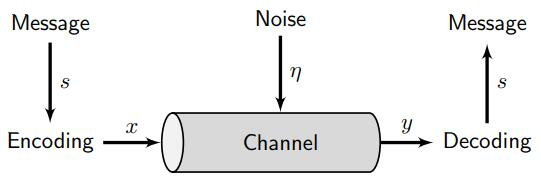
\includegraphics[width = 0.55\linewidth]{./figures/shannon-communicaiton-model.jpg}
	\caption{信息通信模型~\cite{stone2018information}
	}
	\label{fig:communication-model}
\end{figure}

信息通信模型~\cite{stone2018information}由信源消息、编码器、信道、解码器、信宿消息和噪音构成,信源消息(数据)在作为信道输入之前被编码器进行编码;编码后的信源消息在信道中传输,传输过程中会受到噪声影响;解码器从信道中接收到加噪后的信息,解码为信宿消息。Shannon定义的上述通信模型可以描述任何人造或自然的系统间的通信信息量。对任意通信系统,都有:1)信道容量,即可以被信道传输信息的最大量;2)极限受损。即信道中最大的噪音量;3)通过编码,可以达到这两个极限。



\subsection{信息熵}


\begin{definition}
	对于事件集中的某一特定事件~$x$~,~$x$~的概率为~$p(x)$~,则~$x$~的Shannon信息为~$-\text{log}p(x)$~。
\end{definition}
上述定义通常被称为自信息,其表示该事件发生了所需要传递的信息的比特数量。自信息表示了事件所蕴含的信息量,自信息越大,该事件携带的信息量越多,反之越少。而熵表示自信息的平均量,即某一个随机事件变量的所有事件取值发生时,该随机变量的平均Shannon信息量,即

\begin{definition}
随机变量~$X=(x_1,x_2,...,x_n)$~,其概率分布为~$\{p(x_1),p(x_2),....,p(x_n)\}$~,则该随机变量的熵为
\begin{equation}
H(X)=-\sum_{i=1}^{n}p(x_i)log_2p(x_i)
\end{equation}
\end{definition}
在Shannon通信模型中,信源产生的随机事件的熵称为信源熵,信宿产生的随机事件的熵称为信宿熵。信源熵是信源消息变量~$X$~可以表示的平均信息比特数,即平均信息量。但是,上述定义给出的熵是离散变量的熵,对于连续熵的定义,本文不再讨论,可参阅文献~\cite{stone2018information}。

熵是对不确定度的一种度量,当不确定下降时,我们得到了信息,因此信息和熵是一体两面的。上述定义的熵是针对所有离散随机变量的,任意随机变量都存在一个概率分布,使得该随机变量的熵为最大,该分布称为最大熵分布。通过熵的定义可知,当~$n$~个随机事件均匀分布时,该随机变量熵最大,即有

\begin{equation}
H(X)_{Max}=-\sum_{i=1}^{n}p(1/n)log_2p(1/n)
\end{equation}


针对Shannon通信模型,若在信源输入消息,则会对信宿消息的不确定度产生影响,从平均意义上就有平均不确定度的影响,即条件熵。

\begin{definition}
	随机变量~$X=(x_1,x_2,...,x_n)$~是输入,其概率分布为~$\{p(x_1),p(x_2),....,p(x_n)\}$~,随机变量~$Y=(y_1,y_2,...,y_n)$~是输出,其概率分布为~$\{p(y_1),p(y_2),....,p(y_m)\}$~,则输入~$X$~时,~$Y$~的不确定度为
	\begin{equation}
	H(Y/X)=-\sum_{j=1}^{m}p(y_j/x_i)log_2p(y_j/x_i)
	\end{equation}
\end{definition}


\subsection{互信息}

\begin{definition}
变量~$X$~与~$Y$~之间的互信息~$I(X,Y)$~是指,输入~$X$~时的每个随机事件能够提供给~$Y$~的平均信息量,互信息可以表示为
\begin{equation}
I(X,Y)=H(X)-H(X/Y)=H(Y)-H(Y/X)
\end{equation}
\end{definition}

互信息量描述了两个随机变量之间的信息量,可以认为是隐私保护前后,隐私分析前后,不同隐私信息变量间相差的隐私信息量。


%\subsection{结构信息论}

\section{博弈论}
博弈论~\cite{owen2001game,gibbons1992game} 是一个自利参与者间相互作用的数学模型,用于为这些参与者寻找冲突与合作的解决方案。 博弈包含参与者之间的迭代,并且每个参与者在每次迭代中都将执行一个操作。 最后,博弈达到了解决方案(即平衡),所有博弈者都获得了自己最大的收益。 在特定的博弈中,博弈者是理性的,这意味着每个博弈者都会采取行动来响应他人的行动,以获取最大的利益。


\subsection{博弈模型}

一个博弈模型往往有三部分组成,1) 参与者集。博弈中往往包含一定数量的博弈参与者~$n$~;2)策略集合。每个参与者的可选策略集合。3)收益函数。每个用户在每次博弈过程中得到的可以量化的收益后损失。
对于每个参与者而言,由于其策略在博弈开始 的时候就定制好的,描述了每个参与者在任何情况下的执行行动,故其策略是复杂的。一些情况下,由于参与者的可选行动范围是非常小的,但也有时候执行行动的可选集合非常大,如象棋、围棋等,策略就变得异常复杂。

\subsection{策略博弈}
策略博弈是指博弈参与者仅进行一次博弈的博弈模型,根据不同的分类,策略博弈被定义为各种不同的策略博弈。

形式化地,策略博弈模型~$\Gamma=(P,A,u)$~中包含参与者~$P=(P_1,P_2,...,P_n)$~   、所有参与者行为集合~$A=(A_1,A_2,...,A_n)$~和效用函数~$u=(u_1,u_2,...,u_n)$~。称~$n$~个参与者的行为有序集合~$a=(a_1,a_2,...,a_n)$~为行为组态,其中~$a_i \in A_i$~是参与者~$p_i$~在其行为集合~$a_i$~中的一个策略选择。行为组态~$a$~可表示为~$a=(a_i,a_{-i})$~,其中~$a_i$~表示除参与者~$P_i$~之外参与者的策略组合。~$u_i(a_i,a_{-i})$~ 表示参与者~$P_i$~在策略组合~$(a_i,a_{-i})$~ 状态下的效用函数。

\begin{definition}
	在策略博弈模型中,对任意参与者~$P_i \in P$~,其效用函数有
	\begin{equation}
	u_i(a_i,a_{-i}) \geq 	u_i(a_i',a_{-i})
	\end{equation}
	其中~$a_i'\in A_i$~,则称策略组合~$a=(a_1,a_2,...,a_n)$~是该策略博弈的\textbf{Nash均衡}。
\end{definition}


\begin{definition}
	在策略博弈模型中,一个策略~$a_i$~是参与者~$P_i$~的\textbf{占优策略},当且仅当对于该参与者的其他任何策略~$a_i'\neq a_i$~和其他参与者可能的策略集合~$a_{-i}$~中,有
	
	\begin{equation}
	u_i(a_i,a_{-i}) \geq 	u_i(a_i',a_{-i})
	\end{equation}
\end{definition}

\begin{definition}
	当博弈模型中仅有两个参与者的时候,称之为\textit{二人博弈}。
\end{definition}



\begin{definition}
二人博弈中,参与者1与参与者2分别有~$n$~种和~$m$~种可选策略,若参与者1选策略~$i$~,参与者2选策略~$j$~,其中~$i=1,2,...,n,j=1,2,...,m$~,则两个参与者进行博弈,且各自获取到了收益函数。若在一个博弈中,两方参与者一输一赢,且参与者1的收益是~$u_{ij}$~,参与者2的收益是~$-u_{ij}$~,则称该博弈是\textit{二人零和博弈}。
\end{definition}

\begin{definition}
	进一步地,若参与者1与参与者2各自的博弈收益之和是某个常数,则称该博弈是\textit{二人常和博弈}。
\end{definition}

当然,二人博弈的相关概念都可以扩展到多人,即\textit{~$n$~人博弈},\textit{~$n$~人零和博弈}与\textit{~$n$~人常和博弈}。博弈的分类可以根据不同的区分度进行,通常将博弈分为合作博弈与非合作博弈;也可以根据博弈参与者对其他参与者的了解程度分为完美信息博弈和非完美信息博弈。



\subsection{扩展式博弈}

扩展式博弈是策略博弈的一种扩展形式,该博弈模型可以描述参与者所有可能策略的序列,所有参与者在每次策略选择时所选策略,当参与者进行策略选择时对其他参与者策略选择的信息获取,所有策略选择组合对参与者自身的效用函数等不同的信息。扩展式博弈可以将参与者不完全信息表述为策略选择的自然可能性,即自然策略选择。

\begin{definition}
一般的,~$n$~个参与者的扩展式博弈包含以下信息:
\begin{enumerate}
	\item ~$n$~个参与者有限集合~$P=(P_1,P_2,...,P_n)$~;
	\item 一颗有根博弈树;
	\item 博弈树的每个叶子节点有一个~$n$~元组效用函数,表示每个可能的博弈结果都对每个参与者都有一个收益。
	\item 博弈树的非叶子节点有一个含有~$n+1$~个自己的分割,该分割中一个子集称为自然参与者的虚拟参与者,其余~$n$~个子集对应所有理性参与者。每个参与者子集中的节点是参与博弈的所有参与者。
	
	\item 自然参与者的每个节点的输出边上有一个概率分布;
	\item 每个理性参与者的每个节点集合被分割为信息集合,这些信息集合在参与者采取策略选择时,成为其不同的策略决策。
	\item 上述这些信息是每个理性参与者的公共常识。
\end{enumerate}
\end{definition}

类似地,扩展式博弈也可以划分为不同的子类,如完美信息博弈,非完美信息博弈,纯策略博弈,混合策略博弈,重复博弈,非重复博弈。扩展式博弈中有个重要的概念,即子博弈精炼Nash均衡,定义如下:
\begin{definition}
扩展式博弈的策略组合~$a=(a_1,a_2,...,a_n)$~是一个\textbf{子博弈精炼Nash均衡}当且仅当:如果它是原博弈的Nash均衡;它在每一个子博弈上也都构成Nash均衡。
\end{definition}
\subsection{演化博弈}

演化博弈\cite{newton2018evolutionary,smith1982evolution}将经典博弈中参与者的理性假设放宽为有限理性,并引入了群体演化。参与者的策略选择在每一次博弈中不一定是最优的,其可在演化过程中模仿其他参与者的高收益策略,调整其后续博弈策略以提高其收益。演化博弈关注所有参与者策略的动态平衡,其核心在于\textbf{演化稳定策略}。

\begin{definition}
	演化博弈中,若一个被所有个体采用的策略可成功抵抗所有其他策略的少量个体入侵,则此策略就被称为\textbf{演化稳定策略}。形式化地,若策略~$a_e$~满足
	\begin{equation}
	u(a_e,a_e) > u(a_i,a_e), \forall i \ne e 
	\end{equation}
	或
	\begin{equation}
	u(a_e,a_e) > u(a_i,a_e), \forall i \ne e,\\
	u(a_e,a_i) > u(a_i,a_i), \forall i \ne e 
	\end{equation}
	则称策略~$a_e$~为演化稳定策略,其中~$u(a_e,a_i)$~表示当策略~$a_e$~遇到~$a_I$~时, ~$a_e$~的收益。
	
\end{definition}


\section{隐私定义及隐私保护模型}
隐私是一种社会化的概念,最早认为是一种不被打扰的权利,随着数据应用的越来越广泛,场景越来越复杂多样,隐私逐步转变为一种形式化、可量化的概念,需要学术界进行深入研究,以便在数字社会时代更好地理解隐私,更好地保护隐私,更好地应用数据。

\begin{definition}\label{def:privacy}
	隐私是个体或群体隐藏自己身份、有关自己信息,进而有选择性的表达自己的能力。
\end{definition}

上述定义来自Wiki百科,是一种描述性的定义。不同文化背景,不同社会阶层的不同个体,对隐私的边界和内容都不尽一致。不过由此,可以将隐私分为两类,即身份隐私、属性隐私。

\subsection{身份隐私}
\begin{definition}
身份隐私是个体或群体隐藏自己身份的能力。
\end{definition}

在数字中时代,包含大量个人信息的数据被广泛的存储在云端、智能终端、各类应用中,身份隐私就变为在一个数据集中、一个通信系统中个人隐藏自己唯一标识、伪标识信息的能力。可以将身份隐私细分为两类隐私,第一类匿名隐私,即在一个特定群体里,无法区别某个特定个体的身份;第二类关系隐私,即判别一个特定个体是否属于某一个特定群体。
\begin{definition}
	匿名隐私是个体隐藏自己在一个群体里无法被唯一区别出来的能力。
\end{definition}

匿名隐私蕴含着一个背景知识,即已知该个体属于该群体,需要保护其身份。例如需要保护住院病人群体中病人的身份,以保护其不被区别出来是哪一个病人。在基于位置服务、社交网络、基因数据等各类场景中都存在匿名隐私,也需要保护匿名隐私。因此,不同类型的匿名性被形式化定义并扩展,如~$k$~匿名~\cite{sweeney2002k}、~$l$~多样性匿名~\cite{machanavajjhala2007l}、~$t$~邻近匿名~\cite{li2007t}等,特别注意的是匿名性的定义伴随着隐私的量化,即上述匿名隐私中的\textbf{隐私保护强度}的量化。

\begin{definition}
	关系隐私是个体隐藏自己被判断是否属于某一个特定群体成员的能力。
\end{definition}

关系隐私是要求比匿名隐私更强的隐私,即其去掉了匿名隐私中的背景知识假设,对隐私保护的要求更高。例如,某特定的人需要隐藏自己,不让敌手判断出其是否属于住院群体中的一员;某个人也需要保护自己,不让敌手知道自己是否属于某个社交群体。关系隐私还可分类为积极关系隐私和消极关系隐私。
\begin{definition}
	积极关系隐私是个体隐藏自己被判断属于某一个特定群体成员的能力。
\end{definition}

\begin{definition}
	关系隐私是个体隐藏自己被判断不属于某一个特定群体成员的能力。
\end{definition}

\subsection{属性隐私}
属性隐私是一种比匿名隐私假设更弱的隐私要求,即某特定的个体已经被唯一识别出来,需要保护其个人信息,如身高、爱好、政治倾向、疾病状况、疾病易感特性等。

\begin{definition}
	属性隐私是个体或群体隐藏自己信息的能力。
\end{definition}

属性隐私的场景最复杂,也最多样化,不同个体对隐私边界即隐私内容的界定也往往区别于此。正是如此,属性隐私需要更多的、更深入的研究,以提供更加个性化、更加自适应、更加全面的隐私保护。


此外,根据定义~\ref{def:privacy}可知,隐私表达是一种更高的要求,是在保障个人身份隐私和属性隐私的基础上,能够自主可控的表达个人隐私的能力。
\begin{definition}
	隐私表达是个体或群体表达自己身份隐私或属性隐私的能力。
\end{definition}



目前,对匿名隐私的研究较多,关系隐私的研究和属性隐私的研究次之,对隐私表达的研究较少,除了更加具体的形式化表达不同场景下的不同隐私,即形成了隐私的形式化定义,对隐私形式化定义的基础上需要可量化、可比较的方法,即形成了隐私度量。

\subsection{隐私保护模型}

对上述三类隐私定义的实现方法需求,产生了隐私保护机制的研究,如实现~$k$~匿名性的算法~\cite{sweeney2002k},实现差分隐私定义的差分隐私算法~\cite{dwork2006differential},一般的隐私保护模型如图~\ref{fig:ppm-model}所示。

\begin{figure}[htbp]
	\centering
	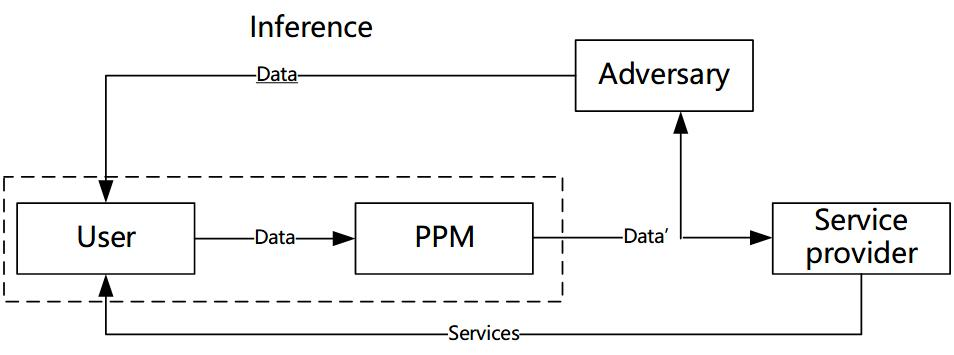
\includegraphics[width = 0.6\linewidth]{./figures/cha1-ppm.jpg}
	\caption{隐私保护模型}
	\label{fig:ppm-model}
\end{figure}

在图~\ref{fig:ppm-model}中,包含用户个人信息的隐私数据通过一定的隐私保护机制进行保护,提交给服务提供者并从其获得数据服务,在此过程中会受到不同能力的敌手的隐私分析。

关于隐私保护机制,针对不同的隐私定义和隐私目标,不同的隐私保护算法被设计出来,形成了\textbf{隐私保护算法研究};同时对因保护机制的能力量化形成了隐私保护机制评价研究,即\textbf{隐私保护强度度量};在敌手针对隐私进行分析的过程中,设计了不同的隐私分析算法,即形成了\textbf{隐私分析研究};同样,对隐私分析强度也需要度量,量化被攻击者的隐私损失,量化敌手的隐私获取量等,即\textbf{隐私分析强度度量研究};数据共享应用的目的是获得较好的数据服务,即数据效用,但隐私保护需求和数据效用需求相互冲突,又相互依赖,需要平衡二者的关系,即产生了\textbf{理性隐私保护研究};在理性隐私保护领域,隐私和效用往往需要能够统一的量化、比较和交换,又进一步产生了\textbf{隐私效用度量研究}。

\section{小结}

本章简要介绍了信息论、博弈论和隐私保护模型的基本知识,其中信息论作为本文的基础性工具,在后续的每一部分都将使用相关概念和方法,以对隐私定义并量化,对隐私保护强度度量和评价,对隐私分析强度进行度量和评价;博弈论作为主要的工具帮助本文在后续章节实现理性的隐私保护方案设计,以动态的、自适应的实现数据隐私保护和数据效用间的平衡;隐私保护模型是本文研究的核心基础,本文的所有研究都围绕该模型展开,包括统一的隐私度量框架、序列型数据属性隐私分析与量化、面向隐私保护的风险自适应访问控制和理性隐私风险访问控制模型。%基础知识
\chapter{基于信息熵的隐私通信模型及度量方法}
\label{chap:entropy-metric-model}

\textit{ }

\textit{本章针对目前隐私量化缺乏对隐私定义、隐私分析、隐私保护等统一的量化框架的问题,基于Shannon信息论的通信框架提出了几种隐私保护信息熵模型\cite{peng2016privacy}。在所提出的度量模型中,将信息拥有者假设为发送方,隐私谋取者假设为接收方,隐私的泄露渠道假设为通信信道;基于该假设,分别引入信息熵、平均互信息量、条件熵及条件互信息等来分别描述隐私保护系统信息源的隐私度量、隐私泄露度量、含背景知识的隐私度量及泄露度量;以此为基础,进一步提出了隐私保护方法的强度和敌手攻击强度的量化,为隐私泄露的量化风险评估提供了一种支撑。}%;最后,针对位置隐私保护的应用场景,给出了具体的信息熵模型及隐私保护机制和攻击强度的度量及分析。}

\section{概述}

隐私保护的研究起步较早,但近年来突然受到产业界和学术界的广泛关注是因为大数据的不期而至,隐私保护成为大数据应用的主要瓶颈,移动网络、社交网络、基于位置服务等新型应用服务的推进,隐私问题更加突出。目前关于隐私保护有两个方向值得关注:一是研究隐私保护算法以更加有效的方式保护隐私;二是通过研究隐私泄露风险分析与评估。隐私保护算法目前主要集中在匿名方法,包括~$k$~匿名、~$l$~多样性匿名和~$T$~接近匿名及其衍生的方法。隐私度量最早起源于相关匿名算法~\cite{sweeney2002k}, 在匿名隐私保护算法的研究过程中,不时有学者关注隐私量化问题,尤其是在定位服务领域,位置匿名及轨迹匿名算法上已有不少隐私度量的相关研究~\cite{shokri2011quantifying,olteanu2017quantifying},因此对于隐私保护算法来说,隐私度量仍需进一步深入研究。然而就目前来说,隐私泄露涉及因素众多,设计有效的隐私保护算法仍是挑战性问题,但政府及企业数据开放共享中迫切的隐私保护需求,促使我们不得不在可用性与隐私泄露之间寻求一种平衡,要解决这个问题,隐私风险分析及评估不失为一种方法。风险分析依然涉及到隐私量化问题,也就是说量化风险评估不失为隐私保护一种可行的解决方案,量化隐私风险必然也涉及隐私度量问题。从这些分析来看,隐私度量的研究具有十分重要的理论意义和应用价值。

信息熵作为信息度量的有效工具,在通信领域已展现出其重要的贡献。隐私作为一种信息,自然可以考虑用熵来量化,为此,不少学者或多或少进行了探索,比如事件熵、匿名集合熵、条件熵等~\cite{serjantov2002towards,diaz2002towards,wagner2018technical},但其研究还较为零散,更多是针对某一具体领域,如位置隐私保护领域,目前尚未形成统一的模型及体系,其应用范围也受到限制,特别是隐私是具有时空性的,与人的主观感受也有关系,不同的人对同一隐私的认同可能不同。 鉴于以上分析,本章旨在参考Shannon信息论的通信框架~\cite{stone2018information},提出几种隐私保护信息熵模型,包括隐私保护基本信息熵模型、含敌手攻击的隐私保护信息熵模型、带主观感受的信息熵模型和多隐私信源的隐私保护信息熵模型。在这些模型中,将信息拥有者假设为发送方,隐私谋取者假设为接收方,隐私的泄露渠道假设为通信信道;基于这样的假设,分别引入信息熵、平均互信息量、条件熵及条件互信息等来分别描述隐私保护系统信息源的隐私度量、隐私泄露度量、含背景知识的隐私度量及泄露度量;以此为基础,进一步提出了隐私保护方法的强度和敌手攻击强度的量化测评,力图为隐私泄露的量化风险评估提供一种理论支持。


\section{相关工作}\label{related work}

信息熵理论是Shannon于1948年提出的,解决了信息的量化和通信的理论基础。较早将信息熵考虑到隐私度量的研究是Diaz等~\cite{diaz2002towards}和Serjantov等~\cite{serjantov2002towards},他们提出了用信息熵来度量匿名通信系统的匿名性,在假定攻击者的目的是确定消息的发送者(或接收者)的真实身份的情况下,系统中每个用户都以一定的概率被猜测为消息的真实发送者(或接收者),将攻击者猜测某用户是真实发送者(或接收者)看成一个随机变量~$X$~,用信息熵~$H(X)=-\sum p(x)\log p(x)$~来量化的随机变量的不确定性可表征为系统的隐私水平。随后,有不少学者将信息熵应用于某些具体领域的隐私度量,如位置服务、社交网络和数据挖掘等领域,对于不同的方案~\cite{serjantov2002towards,shokri2011quantifying,wang2012location},其随机变量的概率表现形式和对熵的处理方式不同。在位置服务领域,2007年,Hoh等~\cite{hoh2007preserving}提出了基于信息熵的隐私度量方法度量轨迹跟踪的不确定度,其中随机变量的概率表现为每个位置实例包含在当前跟踪车辆轨迹的概率。2009年,Ma等~\cite{ma2009measuring}提出在V2X车联网系统中信息熵的隐私度量方法,其中随机变量的概率表现为每个位置信息关联到某特定用户的概率,该方法还考虑了随机变量的概率随着时间的变化而更新的情况,也即攻击者的累积信息对系统隐私的影响。同年,林欣等~\cite{lin2009lbs}针对LBS中的连续查询问题,提出一种连续查询攻击算法,指出匿名集的势不再适合作为查询该算法匿名性的度量,并提出了基于信息熵的度量方法,其中随机变量的概率表现为每个用户~$u_{i}$~是查询~$q$~的真正发出者的概率,信息熵计算为~$H(q)$~,用~$D(q)=2^{H(q)}$~度量为系统的隐私水平。2011年,Shokri等~\cite{shokri2011quantifying}将位置隐私的度量准则分为精确性、确定性和正确性,精确性度量为攻击者猜测事件的置信区间,确定性度量为攻击者猜测的不确定性,正确性度量为攻击者出错的概率,其中精确性的度量是基于信息熵的度量方法,随机变量的概率表现为每个观测事件是真实事件的概率。2012年,Chen等~\cite{chen2012measuring}针对LBS查询隐私进行度量,随机变量的概率表现为攻击者在无背景知识和有背景知识两种情况下的判断用户~$u_{i}$~是查询~$q$~的真实发出者的条件概率,并利用互信息~$I(U|q;<r,t,q>)=H(U|q)-H(U|<r,t,q>)$~度量系统的隐私水平。同年,王彩梅~\cite{wang2012location}等针对LBS中的轨迹隐私保护方法Silent Cascade提出基于信息熵的隐私度量方法,随机变量的概率表现为某用户的每条可能轨迹的概率,特定用户的熵计算为~$H(u_{i})$~,并用标准熵~$D(u_{i})=H(u_{i})/H_{max}(u_{i})$~度量为系统的隐私水平。2014年,文献~\cite{niu2014achieving,olteanu2017quantifying}均采用了信息熵度量了LBS系统的隐私水平。

在社交网络领域,2010年,Ngoc等~\cite{ngoc2010new}针对社交网络隐私泄露的情况,提出了基于信息熵的隐私度量方法,以帮助用户判断所发布信息的隐私水平,其随机变量的概率表现为事件\textit{X}的取值\textit{x}的概率。2012年,Yang等~\cite{yang2012stalking}总结了社交网络中的风险,并利用信息熵和互信息度量的系统的隐私水平。

此外,信息熵在其它领域的隐私度量中也有所涉及,文献~\cite{agrawal2001design,zhan2007quantifying}研究了信息熵用于数据挖掘领域的隐私度量,文献~\cite{edman2007combinatorial}研究了信息熵用于匿名系统领域的隐私度量,文献~\cite{wagner2017evaluating}研究了信息熵基因序列隐私的隐私度量,Wagner等~\cite{wagner2018technical}对当前存在的隐私度量方法进行了综述,根据度量系统的输出将隐私度量方法分成八类,其中不确定度的分类中是根据信息熵来度量的。

综上可知,目前存在的基于信息熵进行隐私度量的理论体系较为零散,缺乏统一的模型基础。针对上述问题,本章试图将隐私保护系统看作一个通信模型,力图探讨较为通用的隐私度量信息熵模型,解决隐私度量的一些基本概念和基础体系。

\section{隐私保护信息熵模型}\label{sec:Entropy model of privacy protection information}

本章的出发点是将信息拥有者假设为发送方,隐私谋取者(敌手)假设为接收方,隐私的泄露渠道假设为通信信道。

发送方拥有的一个信息集称为隐私信源,用随机变量~$X$~表示,~$X$~是由所有的离散基本泄露事件的隐私消息构成的隐私消息空间,即~$\left \{ x_{1},x_{2},...,x_{i},...,x_{n} \right \}$~,其中~$X_{i}(i=1,2,...,n)$~为基本泄露事件的隐私消息;接收方获取的信息集称为隐私信宿,用随机变量~$Y$~表示,~$Y$~是由敌手获取的所有基本隐私消息构成,即~$\left \{y_{1},y_{2},...,y_{j},...,y_{m} \right \}$~,其中~$Y_{j}(j=1,2,...,m)$~为敌手获取的某个隐私消息。相应的,某一种具体的隐私保护算法可以看作是对隐私消息进行转换、编码的方法,它能够对隐私消息进行干扰进而实现对隐私信息的保护,其中隐私保护算法的全体构成隐私保护机制空间,称为隐私保护机制源。敌手在一定背景知识下对隐私信息的挖掘与分析手段称为隐私攻击,所有隐私方法的全体称为隐私攻击空间。

以此假设为基础,本节将基于Shannon信息论的通信框架~\cite{stone2018information}提出几种隐私保护信息熵模型,包括:隐私保护基本信息熵模型、含敌手攻击的隐私保护信息熵模型、带主观感受的信息熵模型和多隐私信源的隐私保护信息熵模型。通过引入隐私信息熵、平均互信息量、条件熵及条件互信息等来分别描述隐私保护系统信息源的隐私度量、隐私泄露度量、含背景知识的隐私度量及泄露度量。

\subsection{隐私保护基本信息熵模型}

这里我们首先假设敌手无任何隐私攻击强度,敌手仅通过信道观测到隐私信息,并只考虑离散单隐私信源的情形。模型定义为
\begin{figure}[htbp]
	\centering
	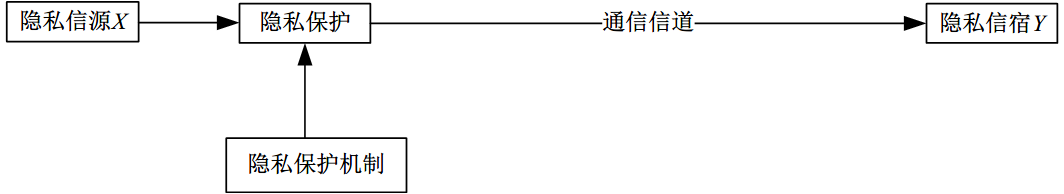
\includegraphics[width = 0.95\linewidth]{./figures/Communication-Model-for-Privacy.png}
	\caption{单隐私信源隐私保护通信模型}
	\label{fig:communication-model-privacy}
\end{figure}

图~\ref{fig:communication-model-privacy}中,设单隐私信源~$X$~的数学模型可以表示为
\begin{equation}
\begin{pmatrix}
X\\ 
P(X)
\end{pmatrix}=\begin{pmatrix}
x_{1} & x_{2} & \cdots  & x_{i} & \cdots  & x_{n}\\ 
p(x_{1})& p(x_{2}) & \cdots & p(x_{i}) & \cdots & p(x_{n})
\end{pmatrix}
\end{equation}
其中~$0\leqslant p(x_{i})\leqslant1$~,~$\sum_{i=1}^{n}p(x_{i})=1$~。同理,隐私信宿~$Y$~的数学模型可表示为
\begin{equation}
\label{eq:single-information-source}
\begin{pmatrix}
Y\\ 
P(Y)
\end{pmatrix}=\begin{pmatrix}
y_{1} & y_{2} & \cdots  & y_{i} & \cdots  & y_{m}\\ 
p(y_{1})& p(y_{2}) & \cdots & p(y_{i}) & \cdots & p(y_{m})
\end{pmatrix}
\end{equation}

针对该模型,定义\textbf{隐私信源熵}~$H(X)$~为
\begin{equation}
H(X)=-\sum_{i=1}^{n}p(x_{i})\log_{2}p(x_{i})
\end{equation}
其中,~$H(X)$~用于刻画隐私信源的平均隐私信息量,也是隐私信源的隐私不确定程度,~$H(X)$~越大,隐私泄露就可能越小,从而它亦可以用于衡量隐私的保护程度,在没有外部条件影响时,该值是一个确定的值。

当隐私信宿~$Y$~在获取隐私信息条件下,关于隐私信源~$X$~的不确定程度,可以引入\textbf{隐私条件熵}$~H(X/Y)$~刻画,其定义为
\begin{equation}
H(X/Y)=-\sum_{j=1}^{m}\sum_{i=1}^{n}p(x_{i}y_{j})\log_{2}p(x_{i}/y_{j})
\end{equation}

该条件熵表示隐私信宿在收到~$Y$~后,隐私信源~$X$~仍存在的不确定程度,该不确定程度是隐私泄露信道的干扰(隐私保护)造成的,即敌手在长期观测隐私信源过程中,由于隐私保护机制的保护下,敌手对隐私信源仍存在一定的不确定。

易证上述的隐私信息熵是满足Shannon信源熵的基本性质。即具有非负性、对称性、扩展性、确定性、可加性、极值性、上凸性等,并满足极大离散熵定理,在此不再赘述。

下面引入\textbf{平均隐私互信息量}$~I(X,Y)$~来刻画信道上隐私泄露程度,定义为
\begin{equation}
I(X;Y)=\sum_{i=1}^{n}\sum_{j=1}^{m}p(x_{i}y_{j})\log_{2}\frac{p(x_{i}/y_{j})}{p(x_{i})}
\end{equation}
其中,~$I(X;Y)$~表示了隐私信源~$X$~和隐私信宿~$Y$~之间交互的平均信息量,即在信道上传送的隐私信息量,它正好可以刻画隐私的整体泄露程度,从而可用于度量隐私的泄露。

\subsection{含敌手攻击的隐私保护信息熵模型}\label{subsec:privacy-preserving-attack}

上节提出的隐私保护基本信息熵模型客观上描述了无敌手攻击或敌手无攻击能力情况下的隐私度量问题。在实际系统中往往存在着隐私攻击分析,敌手可以在一定的背景知识下进行攻击分析,模型定义为图~\ref{fig:Communication-Model-for-Privacy-of-Single}所示模型。
\begin{figure}[htbp]
	\centering
	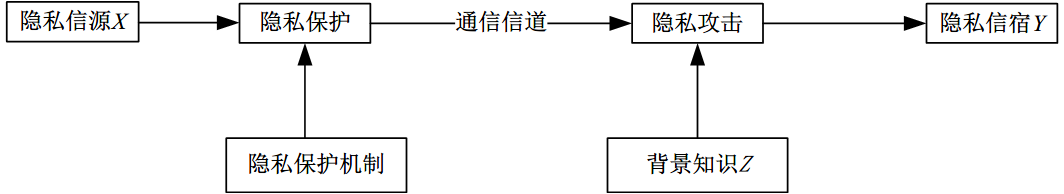
\includegraphics[width = 0.95\linewidth]{./figures/Communication-Model-for-Privacy-of-Single.png}
	\caption{单隐私信源且敌手具备知识背景的隐私保护通信模型}
	\label{fig:Communication-Model-for-Privacy-of-Single}
\end{figure}

在图~\ref{fig:Communication-Model-for-Privacy-of-Single}中,~$Z$~表示背景知识空间,其数学模型亦可定义为
\begin{equation}
\begin{split}
&\begin{pmatrix}
Z\\ 
P(Z)
\end{pmatrix}=\begin{pmatrix}
z_{1} & z_{2} & \cdots  & z_{i} & \cdots  & z_{m}\\ 
p(z_{1})& p(z_{2}) & \cdots & p(z_{i}) & \cdots & p(z_{m})
\end{pmatrix} \\
&0 \leqslant p(z_{k})\leqslant 1,\sum_{k=1}^{l}p(z_{k})=1(k=1,2,...,l)
\end{split}
\end{equation}

攻击者可以利用背景知识~$Z$~加强对隐私进行攻击,对于攻击者来说,可以联合隐私信宿消息~$Y$~和背景知识~$Z$~进行隐私分析攻击,引入\textbf{攻击条件熵}
\begin{equation}
H(X/YZ)=\sum_{i=1}^{n}\sum_{j=1}^{m}\sum_{k=1}^{l}p(x_{i}y_{j}z_{k})\log_{2}p(x_{i}/y_{j}z_{k})
\end{equation}

上述公式中,~$H(X/YZ)$~反映了攻击者在获得隐私信宿消息~$Y$~和背景知识~$Z$~后,关于~$X$~仍存在的不确定度,它实际了可以作为在具有攻击分析的情况下隐私信息的不确定度,亦可以作为隐私保护强度的度量。
进一步定义\textbf{隐私攻击平均互信息}$~I(X;Y/Z)$~
\begin{equation}
I(X;Y/Z)=\sum_{i=1}^{n}\sum_{j=1}^{m}\sum_{k=1}^{l}p(x_{i}y_{j}z_{k})\log_{2}\frac{p(x_{i}z_{k}/y_{j})}{p(x_{i}/z_{k})p(y_{j}/z_{k})}
\end{equation}

上述公式反映了得到~$Z$~的条件下,~$X$~和~$Y$~之间的平均互信息量,即接收方获得的隐私信息量,即可以刻画具有背景知识攻击下的隐私泄露程度。

\subsection{带主观感受的隐私保护信息熵模型}

信息源发生的隐私事件所泄露的隐私信息是客观存在的,但通常对隐私信息是带有主观感受的,不同的隐私信息的重要程度不同或价值不同。本节将权重引入前两节的信息熵模型中,对含有主观感受的隐私信源的隐私信息进行度量。

\textbf{(1) 带主观感受的隐私保护信息熵模型}

针对图~\ref{fig:communication-model-privacy}所述通信模型。隐私信源发出的消息~$X_{i}(i=1,2,...,n)$~,确定一个非负实数作为该消息的重要程度权值,不同的消息,权值越大,重要程度越大。可对该隐私信源建立权值空间
\begin{equation}
\centering
\begin{split}
&\begin{pmatrix}
X\\ 
W(X)
\end{pmatrix}=\begin{pmatrix}
x_{1} & x_{2} & \cdots  & x_{i} & \cdots  & x_{n}\\ 
w(x_{1})& w(x_{2}) & \cdots & w(x_{i}) & \cdots & w(x_{n})
\end{pmatrix} \\
\end{split}
\end{equation}
其中~$w_{i}\geqslant 0(i=1,2,...,n)$~。定义\textbf{隐私加权信源熵}$~H_{w}(X)$~对隐私信源的隐私信息加权平均隐私信息~$~w_{i}(i=1,2,...,n)$~量进行度量,并刻画了隐私信源对隐私消息的主观感受影响信源的隐私信息量。在相对稳定的时间段内,隐私信源对隐私消息的主观感受或偏好一旦固定,隐私加权信源熵是一个确定的值。

\begin{equation}
H_{w}(X)=-\sum_{i=1}^{n}w_{i}p(x_{i})\log_{2}p(x_{i})
\end{equation}

隐私信源加权熵显然有以下性质。
\begin{itemize}
	\item 非负性。无论一个隐私事件的重要程度如何,隐私信源一旦发生了一个隐私事件,其总能提供一定关于隐私信息的信息量。
	\item 连续性。隐私信源发生的隐私事件的概率发生微小的变动,形成另一个隐私信源,变化前后两个隐私信源的加权熵是连续的。该特性对于刻画因时间变化,隐私信源的特性变化是非常有效的。如在某一段时间内,一个人的生活规律是固定的,导致其能够泄露个人隐私的行为模式的概率分布是相对固定的,但随时间的推移,此人的生活规律会连续性的发生微小的变化,进而能够泄露其隐私的行为模式概率分布也发生了微小的变动。但行为发生变化前后关于行为总体的加权熵是连续的。
\end{itemize}

除此之外,隐私信源加权熵还有对称性,均匀性等不同性质,并在隐私保护系统中有相应的实际意义。仅考虑隐私信源对隐私消息的主观感受,定义\textbf{隐私加权条件熵}$~H_{w}(X/Y)$~刻画隐私谋取者对信息拥有者的隐私信息平均不确定程度。
\begin{equation}
H_{w}(X/Y)=-\sum_{i=1}^{n}w_{i}\sum_{j=1}^{m}p(x_{i}y_{j})\log_{2}p(x_{i}/y_{j})
\end{equation}

同样, 仅考虑隐私信源对隐私消息的主观感受,定义\textbf{隐私加权平均互信息}$~I_{w}(X;Y)$~刻画信息拥有者发生了隐私事件之后,在隐私保护机制的保护下,隐私谋取者观测到的隐私事件后接收到关于信息拥有者的隐私信息量。
\begin{equation}
I_{w}(X;Y)=-\sum_{i=1}^{n}w_{i}\sum_{j=1}^{m}p(x_{i}y_{j})\log_{2}\frac{p(x_{i}/y_{j})}{p(x_{i})}
\end{equation}

这里,隐私加权条件熵和隐私加权平均互信息仅考虑了隐私信源对隐私消息的主观感受和偏好,在实际系统中,不仅仅是信息拥有者对自身的隐私信息有不同的主观感受,隐私谋取者对获取到的隐私信息也有不同的主观感受和偏好。故可以进一步探讨通信模型中隐私信宿对隐私消息的主观感受并赋予权值,甚至建立刻画隐私信源和隐私信宿双方偏好的权值矩阵,定义更加符合实际的隐私加权条件熵和隐私加权平均互信息。

\textbf{(2) 带主观感受并含敌手攻击的隐私保护信息熵模型}

在本模型中,仍仅考虑隐私拥有者对其隐私信息的主观感受和偏好。故隐私信源~$X$~的\textbf{隐私加权信源熵}$~H_{w}(X)$~定义如公式。同时定义\textbf{加权攻击条件熵}$~H_{w}(X/YZ)$~隐私信宿在具备攻击强度后对在主观感受的隐私信源隐私信息的平均不确定程度,可以作为隐私保护在敌手攻击下的保护强度度量。
\begin{equation}
H_{w}(X/YZ)=-\sum_{i=1}^{n}w_{i}\sum_{j=1}^{m}\sum_{k=1}^{l}p(x_{i}/y_{j}z_{k})\log_{2}p(x_{i}/y_{j}z_{k})
\end{equation}

在此基础上定义\textbf{隐私攻击加权平均互信息}$~I_w(X;Y/Z)$~表示在得到~$Z$~的条件下,隐私信宿接收到的隐私信息量,具体刻画在具有背景知识条件下隐私泄露的量。
\begin{equation}
I_w(X;Y/Z)=\sum_{i=1}^{n}w_{i}\sum_{j=1}^{m}\sum_{k=1}^{l}p(x_{i}y_{j}{x}'_{k})\log_{2}\frac{p(x_{i}z_{k}/y_{j})}{p(x_{i}/z_{k})p(y_{j}/z_{k})}
\end{equation}

\subsection{多信源的隐私保护信息熵模型}

客观上,系统中的信息拥有者是多个的,其带有隐私信息的隐私事件通过隐私保护机制进行保护。故可建立多隐私信源的隐私保护通信模型,对相互关联的多个信源的隐私信息的保护和攻击进行度量。 如图~\ref{fig:Communication-Model-for-Privacy-of-Multi-Source}所示的无隐私攻击的多隐私信源隐私保护通信模型和图~\ref{fig:Communication-Model-for-Privacy-of-Multi-Source-attacks}所示的带隐私攻击的多隐私信源隐私保护通信模型。

\textbf{(1) 多隐私信源的隐私保护信息熵模型}

\begin{figure}[htbp]
	\centering
	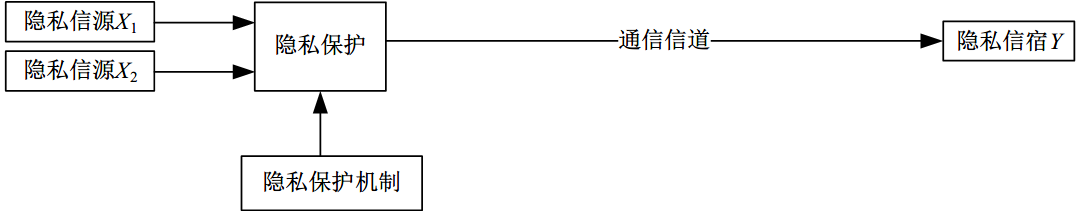
\includegraphics[width = 0.95\linewidth]{./figures/Communication-Model-for-Privacy-of-Multi-Source.png}
	\caption{无隐私攻击的多隐私信源隐私保护通信模型}
	\label{fig:Communication-Model-for-Privacy-of-Multi-Source}
\end{figure}

在图~\ref{fig:Communication-Model-for-Privacy-of-Multi-Source}所示的通信模型中,隐私信源~$X_{1}$~和隐私信源~$X_{2}$~共同构成隐私信源~$X$~,其数学模型为
\begin{equation}
\label{eq:privacy-source1-probability}
\begin{split}
&\begin{pmatrix}
X_{1}\\ 
P(X_{1})
\end{pmatrix}=\begin{pmatrix}
x_{11} & x_{12} & \cdots  & x_{1i_{1}} & \cdots  & x_{1n_{1}}\\ 
p(x_{11})& p(x_{12}) & \cdots & p(x_{1i_{1}}) & \cdots & p(x_{1n_{1}})
\end{pmatrix} \\
&0\leqslant p(x_{i_{1}})\leqslant 1,\sum_{i_{1}=1}^{n_{1}}p(x_{i_{1}})=1(i_{1}=1,2,...,n_{1})
\end{split}
\end{equation}
\begin{equation}
\label{eq:privacy-source2-probability}
\begin{split}
&\begin{pmatrix}
X_{2}\\ 
P(X_{2})
\end{pmatrix}=\begin{pmatrix}
x_{21} & x_{22} & \cdots  & x_{2i_{2}} & \cdots  & x_{2n_{2}}\\ 
p(x_{21})& p(x_{22}) & \cdots & p(x_{2i_{2}}) & \cdots & p(x_{2n_{2}})
\end{pmatrix} \\
&0\leqslant p(x_{i_{2}})\leqslant 1,\sum_{i_{2}=1}^{n_{2}}p(x_{i_{2}})=1(i_{2}=1,2,...,n_{2})
\end{split}
\end{equation}

隐私信宿~$Y$~的数学模型如公式~\ref{eq:single-information-source}所述,定义\textbf{多源联合隐私信源熵}$~H(X_{1}X_{2})$~,该信源熵刻画的多个带关联的隐私拥有者的隐私信息的量。
\begin{equation}
H(X_{1}X_{2}) = -\sum_{i_{1}=1}^{n_{1}}\sum_{i_{2}=1}^{n_{2}}p(x_{i_{1}}x_{i_{2}})\log_{2}p(x_{i_{1}}x_{i_{2}})=H(X_{1})+H(X_{2}/X_{1})
\end{equation}
已知隐私信宿~$Y$~条件下对隐私信源~$X$~的\textbf{多源联合隐私条件熵}为~$H(X/Y)=H(X_{1}X_{2}/Y)=H(X_{1}X_{2}Y)-H(Y)$~。该定义刻画的是多个带关联的信息拥有者发生的隐私事件在隐私保护后,隐私信息获取者对被保护的隐私事件进行观测后其对各信息拥有者的隐私信息的平均不确定程度。

同时,定义\textbf{多源联合平均互信息}$~I(X_{1}X_{2};Y)$~刻画多个带关联的信息拥有者发生的隐私事件在隐私保护后,隐私信息谋取者通过观测被保护隐私事件后获取的各信息拥有者的隐私信息量。
\begin{equation}
I(X_{1}X_{2};Y)=\sum_{i_{1}=1}^{n_{1}}\sum_{i_{2}=1}^{n_{2}}\sum_{j=1}^{m}p(x_{i_{1}}x_{i_{2}}y_{j})\log_{2}\frac{p(x_{i_{1}}x_{i_{2}}/y_{j})}{p(x_{i_{1}}x_{i_{2}})}
\end{equation}

\textbf{(2) 多隐私信源带隐私攻击的隐私保护信息熵模型}

在~\ref{subsec:privacy-preserving-attack}节所提带隐私攻击的隐私保护信息熵模型基础上,引入多个带关联的信息拥有者,构成新的关联的多隐私信源,并可进一步构建多隐私信源带隐私攻击的隐私保护信息熵模型,其通信模型如图~\ref{fig:Communication-Model-for-Privacy-of-Multi-Source-attacks}所示。

\begin{figure}[htbp]
	\centering
	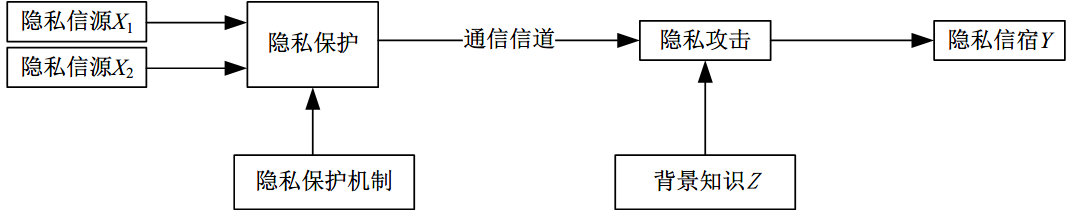
\includegraphics[width = 0.95\linewidth]{./figures/Communication-Model-for-Privacy-of-Multi-Source-attacks.png}
	\caption{带隐私攻击的多隐私信源隐私保护通信模型}
	\label{fig:Communication-Model-for-Privacy-of-Multi-Source-attacks}
\end{figure}

图~\ref{fig:Communication-Model-for-Privacy-of-Multi-Source-attacks}所述通信模型的信源数学模型如公式~\ref{eq:privacy-source1-probability}和~\ref{eq:privacy-source2-probability},隐私信宿~$Y$~的数学模型如公式~\ref{eq:single-information-source}所述。该模型下的\textbf{多源联合信源熵}$~H(X)=H(X_{1}X_{2})$~,\textbf{多源联合隐私攻击条件熵}$~H(X_{1}X_{2}/YZ)$~和\textbf{多源联合隐私攻击条件平均互信息}$~I(X_{1}X_{2};Y/Z)$~,其中多源联合隐私攻击条件熵表示的在已知背景知识攻击下接收者对联合隐私信源的隐私信息的不确定度; 多源联合隐私攻击条件平均互信息表示在已知背景知识攻击下接收者收到的联合隐私信源隐私消息所含的隐私信息量,即有
\begin{equation}
\begin{split}
&H(X_{1}X_{2}/YZ)=H(X_{1}X_{2}YZ)-H(YZ)\\
&I(X_{1}X_{2};Y/Z)=H(X_{1}X_{2})-H(X_{1}X_{2}Y/Z)
\end{split}
\end{equation}

\section{隐私度量方法}\label{Privacy measures}
应用信息熵和平均互信息对隐私信息进行度量,并以此为基础对隐私保护机制的有效性建立评价方法,同时对隐私保护机制对隐私攻击手段的抗攻击强度建立测评方法。

\subsection{隐私信息的熵度量模型}

针对隐私保护基本信息熵模型,直观地可以用条件熵和互信息在该模型下,对隐私保护机制保护下的隐私进行度量。

针对某一隐私信源,可以应用不同的隐私保护机制对隐私信源发送的隐私消息进行保护,调整能够让隐私信宿接收到的消息的概率分布,改变信宿的熵。以隐私信宿的视角,在接收到被保护后的隐私消息,仍对隐私信源的隐私信息有一个平均不确定程度,这个程度应用隐私条件熵~$H(X/Y)$~做量化。记应用某一具体隐私保护机制~$p_{i}$~的对隐私信源~$X$~发送的消息件进行保护后的隐私条件熵为~$H_{P_{i}}(X/Y)$~,则期望该条件熵尽可能大。

平均互信息刻画的是经过信息传输后,信宿所接收到的平均信息量。隐私平均互信息~$I(X;Y)$~表示的是隐私信源~$X$~在隐私保护机制的保护下隐私消息被隐私信宿~$Y$~所接收到的平均隐私信息量。记应用某一具体隐私保护机制~$P_{i}$~的对隐私信源~$X$~发送的消息件进行保护后,隐私信宿~$Y$~接收到的隐私信息为~$I_{P_{i}}(X;Y)$~,则期望该隐私互信息能尽可能小。

\begin{property}
应用隐私条件熵和隐私互信息进行隐私度量,具有一致性。
\end{property}
\begin{proof}
	由公式知
	\begin{equation}
	\begin{split}
	I(X;Y)&=\sum_{i=1}^{n}\sum_{j=1}^{m}p(x_{i}y_{j})\log_{2}\frac{p(x_{i}/y_{j})}{p(x_{i})}\\
	&=\sum_{i=1}^{n}\sum_{j=1}^{m}p(x_{i}y_{j})\log_{2}\frac{1}{p(x_{i})}-\sum_{i=1}^{n}\sum_{j=1}^{m}p(x_{i}y_{j})\log_{2}\frac{1}{p(x_{i}/y_{j})}\\
	&=\sum_{i=1}^{n}p(x_{i})\log_{2}\frac{1}{p(x_{i})}-\sum_{i=1}^{n}\sum_{j=1}^{m}p(x_{i}y_{j})\log_{2}\frac{1}{p(x_{i}/y_{j})}\\
	&=H(X)-H(X/Y)
	\end{split}
	\end{equation}
	
	故有~$I(X;Y)=H(X)-H(X/Y)$~,易知隐私信源熵是一个确定的值,隐私条件熵越大,则隐私平均互信息越小。
\end{proof}


针对含敌手攻击的隐私保护信息熵模型,隐私度量主要是对隐私信宿本身含有的隐私信息量;敌手在背景知识条件下对发送者的隐私信息进行攻击时,发送者隐私信息的保护强度;以及在敌手攻击下,信息拥有者所泄露的隐私信息量。

隐私信宿本身含有的隐私信息量可用隐私信源熵~$H(X)$~的大小进行度量,其表示信息拥有者隐私信息的固有量的多少,一旦隐私信宿确定,则此隐私信宿所拥有的隐私信息量就是一个确定的值。

系统隐私度量综合考虑经过隐私保护和隐私攻击后,在一定背景知识条件下,隐私谋取者对信息拥有者的隐私信息的不确定程度~$H(X/YZ)$~;以及隐私谋取者观测信息拥有者发生的隐私事件所包含的隐私信息量~$I(X;Y/Z)$~。系统中应用隐私保护机制~$P_{i}$~进行隐私保护和隐私攻击~$a_{r}$~进行隐私攻击,则分别记~$H_{P_{i},A_{r}}(X/YZ)$~和~$I_{P_{i},A_{r}}(X;Y/Z)$~作为系统在抵抗攻击~$a_{y}$~下采用~$P_{i}$~的隐私信息泄露的隐私度量值。

\subsection{隐私保护机制强度度量}
\textbf{(1)隐私保护基本信息熵模型下的隐私保护机制强度度量}

应用隐私保护机制对信息拥有者的隐私信息进行保护,~$H_{w}(X/Y)$~目标是使隐私信息尽可能少的被隐私谋取者所获得,即期望通过某种隐私保护机制,使得隐私谋取者得到的信息量~$I(X;Y)$~尽可能小,最好是0。
\begin{definition}
	\label{def:perfec-privacy-preserving}
	若在某种隐私保护机制的保护下,隐私平均互信息~$I(X;Y)=0$~(隐私信宿从隐私信源接收到的隐私信息量为0),则称该隐私保护机制对此信源是\textbf{完全隐私保护}的。
\end{definition}

\begin{definition}
\label{def:partial-ordering}	
	 对同一隐私信源~$X$~分别应用隐私保护机制~$P_{i}$~和~$P_{j}$~对隐私消息进行保护,若\\~$H_{P_{i}}(X/Y)<H_{P_{j}}(X/Y)~$(或~$I_{P_{i}}(X;Y)>I_{P_{j}}(X;Y)$~),则称隐私保护机制~$P_{j}$~比隐私保护机制~$p_{i}$\textbf{隐私保护有效性好},简记偏序关系~$P_{i}\prec P_{j}$~。若~$H_{P_{i}}(X/Y)=H_{P_{j}}(X/Y)~$(或~$I_{P_{i}}(X;Y)=I_{P_{j}}(X;Y)$~),则称隐私保护机制~$P_{i}$~与隐私保护机制~$P_{j}$\textbf{隐私保护有效性相等},简记等价关系~$P_{i}\cong P_{j}$~。
\end{definition}

\begin{theorem}
	\label{thm:distance-properties}
	设隐私保护机制有效性偏序关系与等价关系如定义~\ref{def:partial-ordering}所定义,则偏序关系具有可传递性,等价关系具有自反性,可传递性,对称性。
\end{theorem}

\begin{proof}
	若有~$P_{i}\prec P_{j},P_{j}\prec P_{k}$~,则按照定义,对于隐私条件熵有~$H_{P_{i}}(X/Y)< H_{P_{j}}(X/Y)~$和~$H_{P_{j}}(X/Y)< H_{P_{k}}(X/Y)$~,故~$H_{protection_{i}}(X/Y)< H_{protection_{k}}(X/Y)$~,进而有~$P_{i}\prec P_{k}$~;对于隐私互信息有~$I_{P_{i}}(X;Y)>I_{P_{j}}(X;Y)$~和~$I_{P_{j}}(X;Y)>I_{P_{k}}(X;Y)$~,故~$I_{P_{i}}(X;Y)>I_{P_{k}}(X;Y)$~,进而有~$P_{i}\prec P_{k}$~。
	
	证毕偏序关系的可传递性。类似地,易证等价关系的三个特性。
\end{proof}


\begin{definition}[隐私保护有效性距离]
	\label{def:privacy-preserving-distance} 
	在隐私保护基本信息熵模型下, 对同一隐私信源~$X$~分别应用隐私保护机制~$P_{i}$~和~$P_{j}$~对隐私消息进行保护,隐私信宿接收到的隐私信息量分别为~$I_{P_{i}}(X;Y)$~和~$I_{P_{j}}(X;Y)$~,则两种隐私保护机制的有效性距离为~$D_{i}=\left | I_{P_{i}}(X;Y)-I_{P_{j}}(X;Y) \right |~$~。
\end{definition}

在隐私保护基本信息熵模型下,隐私保护有效性距离刻画的是保护同一隐私信息的两种不同隐私保护机制有效性差异性大小。显然,~$D_{i}$~越小,两种隐私保护算法的有效性差异越小;~$D_{i}$~越大, 两种隐私保护算法的有效性差异越大。

\textbf{(2) 含敌手攻击的隐私保护机制强度度量}

在实际的系统中,应用隐私保护机制对信息拥有者的隐私信息进行保护,目标是即使遭受敌手的各类隐私攻击,仍使得信息拥有者的隐私信息尽可能少的被隐私谋取者所获得,即期望通过某种隐私保护机制抗敌手在一定背景知识下的隐私攻击,使得隐私谋取者得到的隐私信息量~$I(X;Y/Z)$~尽可能的小,最好是0。

\begin{definition}
	\label{def:perfect-privacy-preserving}
	 对于带敌手攻击的隐私保护系统,若~$I(X;Y/Z)=0$~,即在敌手在拥有背景知识~$Z$~的攻击下,隐私保护机制能够使得信息拥有者的隐私信息泄露量为0,则称隐私系统是\textbf{完美隐私保护}的。
\end{definition}


\begin{definition}
	\label{def:privacy-preserving-performance}
	对同一隐私信源~$X$~,其与隐私信宿~$Y$~进行通信过程中受到敌手应用隐私攻击进行攻击~$A_{r}$~,系统分别应用隐私保护机制~$P_{i}$~和~$P_{j}$~对隐私消息进行保护,若~$H_{P_{i},A_{r}}(X/YZ)<H_{P_{j},A_{r}}(X/YZ)~$(~$I_{P_{i},A_{r}}(X;Y/Z)<I_{P_{j},A_{r}}(X;Y/Z)$~),则称在抗~$A_{r}$~攻击下,隐私保护机制~$P_{j}$~比隐私保护机制~$P_{i}$\textbf{隐私保护有效性好},简记偏序关系~$P_{i}(A_{r})\prec P_{j}(A_{r})$~。若~$H_{P_{i},A_{r}}(X/YZ)=H_{P_{j},A_{r}}(X/YZ)~$(~$P_{P_{i},A_{r}}(X;Y/Z)=I_{P_{j},A_{r}}(X;Y/Z)$~),则称隐私保护机制~$P_{i}$~与隐私保护机制~$P_{j}$\textbf{隐私保护有效性}相等,简记等价关系~$P_{i}(A_{r})\cong P_{j}(A_{r})$~。
\end{definition}

\begin{definition}[抗隐私攻击的隐私保护有效性距离]
	\label{def:privacy-preserving-performance-distance}
	在含敌手攻击的隐私保护信息熵模型中,对同一隐私信源~$X$~,针对该信源的隐私消息有隐私攻击~$A_{r}$~,若在该隐私攻击下分别应用隐私保护机制~$P_{i}$~和~$P_{j}$~进行保护,隐私信源~$Y$~在该攻击下接收到的隐私信息量分别为~$I_{P_{i},A_{r}}(X;Y/Z)$~和~$I_{P_{j},A_{r}}(X;Y/Z)$~,则称两种隐私保护机制在隐私攻击~$A_{r}$~下的有效性距离为~$D_{i}(A_{r})=\left | I_{P_{i},A_{r}}(X;Y/Z)-I_{P_{j},A_{r}}(X;Y/Z) \right |~$~。
\end{definition}

\subsection{敌手隐私攻击强度度量}
在含敌手攻击的隐私保护信息熵模型中, 抗隐私攻击的隐私保护有效性距离刻画的是保护同一隐私信息的两种不同隐私保护机制在同一种隐私攻击下的有效性差异性大小。显然~$D_{i}(A_{r})$~越小,两种隐私保护算法的有效性差异越小;~$D_{i}(A_{r})$~越大, 两种隐私保护算法的有效性差异越大。

\begin{definition}
	\label{def:relation-equivalence2}
	 对同一隐私信源~$X$~,其与隐私信宿~$Y$~进行通信过程中应用隐私保护机制~$p_{i}$~进行隐私保护,并分别受到敌手应用隐私攻击~$A_{r}$~和~$A_{\alpha }$~进行攻击,若~${{H}_{{{P}_{i}},{{A}_{r}}}}(X/YZ)<{{H}_{{{P}_{i}},{{A}_{q}}}}(X/YZ)~$ (${{I}_{{{P}_{i}},{{A}_{r}}}}(X;Y/Z)>{{I}_{{{P}_{i}},{{A}_{q}}}}(X;Y/Z)$~),则称在隐私保护机制的保护下, 隐私攻击~$A_{r}$~比隐私攻击~$A_{\alpha }$~的隐私攻击有效性更强,简记偏序关系。若~$H_{P_{i},A_{r}}(X/YZ)<H_{P_{i},A_{q}}(X/YZ)~$(~$I_{P_{i},A_{r}}(X,Y/Z)<I_{P_{i},A_{q}}(X,Y/Z)$~),则称在隐私保护机制~$P_{i}$~的保护下, 隐私攻击~$A_{r}$~与隐私攻击~$A_{\alpha }$~的\textbf{隐私攻击有效性相同},简记等价关系~$A_{r}(P_{i})\cong A_{q}(P_{i})$~。
\end{definition}

\begin{theorem}
	\label{thm:relation-equivalence}
	若偏序关系和等价关系如定义\label{def:relation-equivalence1}或定义~\ref{def:relation-equivalence2}所定义,则该偏序关系满足传递性,该等价关系满足自反性,对称性,可传递性。 
\end{theorem}

\begin{proof}
 略。
\end{proof}


\begin{definition}[隐私攻击有效性距离]
	\label{def:privacy-attack-distance}
	在含敌手攻击的隐私保护信息熵模型中,对同一隐私信源~$X$~的隐私消息应用隐私保护机制~$P_{i}$~进行保护,并有隐私攻击~$A_{r}$~和~$A_{\alpha}$~分别进行隐私攻击,隐私信源~$Y$~在不同攻击下接收到的隐私信息量分别为~$I_{P_{i},A_{r}}(X;Y/Z)$~和~$I_{P_{i},A_{q}}(X;Y/Z)$~,则称两种隐私攻击针对隐私保护机制~$P_{i}$~的有效性距离为
\begin{equation}
D_{i}(P_{i})=\left | I_{P_{i},A_{r}}(X;Y)-I_{P_{i},A_{q}}(X;Y) \right |
\end{equation}
\end{definition}

在含敌手攻击的隐私保护信息熵模型中, 隐私攻击有效性距离刻画的是针对同一种隐私保护机制的两种攻击方法的有效性及攻击强度差异性大小。~$D_{i}(P_{i})$~越小,两种隐私攻击的有效性和攻击强度差异越小;~$D_{i}(P_{i})$~越大, 两种隐私攻击的有效性和攻击强度差异越大。

在隐私保护系统中,敌手在实施攻击时通常具备一定的背景知识,假定背景知识空间为~$Z$~,则敌手截获通信系统的消息,背景知识总能提供一定关于隐私信息的相关信息。

\begin{theorem}
	\label{thm:privacy-attack-performance}
	在带敌手攻击的隐私保护通信模型中,隐私信宿~$X$~发送隐私消息,经过隐私保护和隐私攻击,被隐私信宿~$Y$~接收,若敌手已知背景知识空间~$Z$~,则~$I(X;Y)\leqslant I(X;YZ)$~。
\end{theorem} 

\begin{proof}
由平均互信息的计算方程知
\begin{equation}
\label{eq:mutual-information1}
I(X;Y) =H(X)-H(X/Y)
\end{equation}
\begin{equation}
\label{eq:mutual-information2}
I(X;YZ) =H(X)-H(X/YZ)
\end{equation}
令公式~\ref{eq:mutual-information2}减去公式~\ref{eq:mutual-information1},得到
\begin{equation}
I(X;YZ)-I(X;Y) =H(X/Y)-H(X/YZ)
\end{equation}

由于~$H(X/Y) \geqslant H(X/YZ)$~,故~$H(X/Y)- H(X/YZ)\geqslant0$~,有~$I(X;YZ)\geqslant I(X;Y)$~。
\end{proof}

该定理说明敌手在一定背景知识进行隐私攻击与分析, 敌手获得的隐私信息不少于其无背景知识情况下所能获得的隐私信息。同时也为隐私保护提供了一个方向,即尽可能使得敌手截取的隐私消息与其拥有背景知识关联程度尽可能小,从而最大限度的保护隐私信息。


上文讨论了隐私保护基本信息熵模型及其含敌手攻击情况下的隐私保护机制及隐私攻击评价,给出了隐私保护和隐私攻击评价的相关定义、定理和证明。鉴于隐私保护基本信息熵模型和含敌手攻击的隐私保护信息熵模型的基础性,针对这两个模型的评价方法可以通过有效扩展,直接或间接应用于其他隐私保护信息熵模型。

定义~\ref{def:perfec-privacy-preserving}所述完全隐私保护定义蕴含的隐私保护目标是在无敌手环境或敌手无隐私攻击强度情况下,系统对隐私保护机制的期望,可表示隐私保护机制设计的目标。该期望或隐身保护机制设计目标同样适用于其他无敌手隐私保护信息熵模型,故该定义可扩展于无敌手的带主观感受的隐私保护信息熵模型和无敌手的多隐私信源的隐私保护信息熵模型。类似的,定义~\ref{def:partial-ordering}、定义~\ref{def:privacy-preserving-distance}和定理~\ref{thm:distance-properties}亦可通过引入隐私敏感偏好、多隐私信源联合,进而应用于这两种模型。

定义~\ref{def:perfect-privacy-preserving}所述完美隐私保护是在敌手进行隐私攻击时隐私保护机制设计的目标,该目标是一般隐私系统的通用性目标,同样适用于其他隐私保护信息熵模型。定义~\ref{def:privacy-preserving-performance}和定义	~\ref{def:privacy-preserving-performance-distance}是在受到一定隐私攻击条件下,对不同隐私保护机制效果的评价,该评价方法相对信源模型独立,故可进行一定的扩展应用到其他隐私保护信息熵模型中,如引入隐私敏感偏好并应用带权条件信息熵或带权条件互信息的比较,应用于带主观感受并含敌手攻击的隐私保护信息熵模型。

同样,定义~\ref{def:relation-equivalence2}、定义~\ref{def:privacy-attack-distance}、定理~\ref{thm:relation-equivalence}和定理~\ref{thm:privacy-attack-performance},经过相应的扩展和推广,可以很方便的应用于其他模型中。

%\section{隐私度量应用与分析}\label{instance analysis}
%
%文中提出的隐私保护信息熵模型及其度量方法可适用于多种场景,现基于一个简单的位置隐私保护场景对该模型进行分析。假设某用户~$u$~在一个被划分为\textit{M}块的区域内移动,记~$r=\left \{ r_{1},r_{2},\cdots,r_{M} \right \}$~为\textit{M}块不同区域的集合,攻击者的目的是确定该用户所在的真实位置。
%\subsection{位置隐私保护基本模型}
%对应于含敌手攻击的隐私保护信息熵模型,隐私信源为用户可能所处的位置分布~$r$~,随机变量~$r$~表示用户~$u$~处于一位置区域,该变量的取值表示用户~$u$~处于具体区域~$r_{i}$~,用~$\left \{ r_{1},r_{2},\cdots,r_{M} \right \}$~表示用户所处的位置区域空间,各区域的概率为~$p(r_{i})$~,有~$0\leqslant p(r_{i})\leqslant 1$~,~$\sum_{i=1}^{M}p(r_{i})=1$~,该位置分布~$r$~的概率模型可以表示为
%
%\begin{equation}
%\begin{pmatrix}
%R\\ 
%P(R)
%\end{pmatrix}=\begin{pmatrix}
%r_{1} & r_{2} & \cdots  & r_{i} & \cdots  & r_{M}\\ 
%p(r_{1})& p(r_{2}) & \cdots & p(r_{i}) & \cdots & p(r_{M})
%\end{pmatrix}
%\end{equation}
%
%用户的真实位置分布信息是隐私信息,为防止攻击者直接获取用户所处的真实区域,需要对用户的位置分布~$r$~进行保护,经过位置隐私保护机制(包括位置泛化、取假名、隐藏或添加虚拟位置等)对位置分布~$r$~进行隐私保护处理后,变成可被攻击者直接观测到的可观测位置分布~${R}'$~,同位置分布~$r$~,易知~${R}'=\left \{ {r}'_{1},{r}'_{2},\cdots ,{r}'_{{M}'} \right \}$~,其中~${r}'_{i}$~表示用户~$u$~的经过隐私保护后可被攻击者观测到的所在区域, 可观测位置分布~${R}'$~的概率模型为
%\begin{equation}
%\begin{pmatrix}
%R{}'\\ 
%P({R}')
%\end{pmatrix}=\begin{pmatrix}
%{r}'_{1} & {r}'_{2} & \cdots  & {r}'_{i} & \cdots  & {r}'_{{M}'}\\ 
%p({r}'_{1})& p({r}'_{2}) & \cdots & p({r}'_{i}) & \cdots & p({r}'_{{M}'})
%\end{pmatrix}
%\end{equation}
%\begin{equation}
%0\leq p({r}'_{i})\leq1,\sum_{i=1}^{M{}'}p({r}'_{i})=1
%\end{equation}
%
%攻击者获取到可观测位置分布~$r{}'$~后,结合背景知识,对用户~$u$~进行位置攻击,即得到攻击者对用户~$u$~的推断位置~$\hat{R}$~,同位置分布~$r$~,易知~$\hat{R}=\left \{ \hat{r_{1}},\hat{r_{2}},\cdots ,\hat{r}_{\hat{M}} \right \}$~,其中~$\hat{r_{i}}$~表示攻击者猜测用户~$u$~所处区域为真实区域, 其概率模型为
%
%\begin{equation}
%\begin{pmatrix}
%\hat{R}\\ 
%P(\hat{R})
%\end{pmatrix}=\begin{pmatrix}
%\hat{r}_{1} & \hat{r}_{2} & \cdots  & \hat{r}_{i} & \cdots  & \hat{r}_{\hat{M}}\\ 
%p(\hat{r}_{1})& p(\hat{r}_{2}) & \cdots & p(\hat{r}_{i}) & \cdots & p(\hat{r}_{\hat{M}})
%\end{pmatrix}
%\end{equation}
%\begin{equation}
%0\leq p(\hat{r}_{i})\leq 1,\sum_{i=1}^{\hat{M}}p(\hat{r}_{i})=1
%\end{equation}
%
%图~\ref{fig:Communication-Model-for-Privacy-of-location}表示位置隐私保护场景的通信模型,可以看作含敌手攻击的隐私保护信息熵模型的一个具体实例。
%
%\begin{figure}[htbp]
%	\centering
%	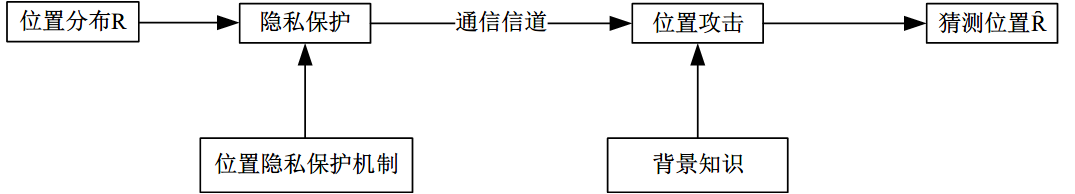
\includegraphics[width = 0.95\linewidth]{./figures/Communication-Model-for-Privacy-of-location.png}
%	\caption{位置隐私保护场景通信模型}
%	\label{fig:Communication-Model-for-Privacy-of-location}
%\end{figure}
%
%\subsection{不同隐私保护机制强度量化对比}\label{4.2}
%
%在初始阶段,用户~$u$~处于一个真实区域~$r_{i}$~,则该用户处于区域~$r_{i}$~的概率为1,处于其它区域的概率为0,具体为
%
%\begin{equation}
%\begin{pmatrix}
%R\\ 
%P(R)
%\end{pmatrix}=\begin{pmatrix}
%r_{1} & r_{2} & \cdots  & r_{i} & \cdots  & r_{M}\\ 
%0 & 0 & \cdots  & 1 & \cdots  & 0
%\end{pmatrix}
%\end{equation}
%
%此时,隐私信源熵即位置分布~$r$~的熵为~$H(R)=-\sum_{i=1}^{M}p(r_{i})\log p(r_{i})=0$~。
%
%\textbf{(1) 弱隐私保护强度的隐私度量}
%
%当系统采用的位置隐私保护机制是位置泛化时,我们取用户~$u$~的发布位置从区域~$r_{i}$~泛化到~$\left \{ r_{i-1},r_{i},r_{i+1},r_{i+2} \right \}$~,可得到可观测位置分布的概率模型为
%\begin{equation}
%\begin{pmatrix}
%{R}'\\ 
%P({R}')
%\end{pmatrix}=\begin{pmatrix}
%{r}'_{1} & \cdots  & {r}'_{i-1} & {r}'_{i} & {r}'_{i+1}  & {r}'_{i+2} & \cdots & {r}'_{{M}'} \\ 
%0 & \cdots & \frac{1}{4} & \frac{1}{4} & \frac{1}{4}  & \frac{1}{4} & \cdots & 0
%\end{pmatrix}
%\end{equation}
%
%我们可以用~$H({R}')=-\sum_{i=1}^{{M}'}p({r}'_{i})\log p({r}'_{i})=2$~表示可观测位置分布的熵,等同于含敌手攻击的隐私保护信息熵模型下的熵~$H(X/Y)$~。
%
%攻击者在获取到可观测位置分布后,结合其所拥有的背景知识进行分析,在一定的背景知识下,分析得到对用户~$u$~的推断位置分布的概率模型如下:
%
%\begin{equation}
%\begin{pmatrix}
%\hat{R}\\ 
%P(\hat{R})
%\end{pmatrix}=\begin{pmatrix}
%\hat{r}_{1} & \cdots  & \hat{r}_{i-1} & \hat{r}_{i} & \hat{r}_{i+1}  & \hat{r}_{i+2} & \cdots & \hat{r}_{\hat{M}} \\ 
%0 & \cdots & \frac{1}{4} & \frac{1}{2} & \frac{1}{8}  & \frac{1}{8} & \cdots & 0
%\end{pmatrix}
%\end{equation}
%
%此时我们可得~$H(\hat{R})=-\sum_{i=1}^{\hat{M}}p(\hat{r}_{i})\log p(\hat{r}_{i})=1.75
%~$~表示攻击者在具有背景知识的条件下对用户所在位置的不确定度的度量,等同于敌手攻击的隐私保护信息熵模型下的熵~$H(X/YZ)$~。
%
%\textbf{(2) 强隐私保护强度的隐私度量}
%
%当我们取泛化位置区域变大时,即隐私保护手段变强后,我们取用户~$u$~的发布位置从区域~$\left \{ r_{i-1},r_{i},r_{i+1},r_{i+2} \right \}$~变到~$\left \{ r_{i},r_{i+1},\cdots,r_{i+7} \right \}$~,可观测位置分布的概率模型为
%\begin{equation}
%\begin{pmatrix}
%{R}'\\ 
%P({R}')
%\end{pmatrix}=\begin{pmatrix}
%{r}'_{1} & \cdots & {r}'_{i}  & \cdots & {r}'_{i+7} & \cdots & {r}'_{{M}'}\\ 
%0 & \cdots  & \frac{1}{8} & \cdots  & \frac{1}{8} & \cdots  & 0
%\end{pmatrix}
%\end{equation}
%
%得到~$H({R}')=-\sum_{i=1}^{{M}'}p({r}'_{i})\log p({r}'_{i})=3$~表示可观测位置分布的熵,攻击者在相同的背景知识下,分析得到对用户~$u$~的推断位置分布的概率模型为
%\begin{equation}
%\begin{pmatrix}
%\hat{R}\\ 
%P(\hat{R})
%\end{pmatrix}=\left( \begin{array}{cccccccccccc} 
%\hat{r}_{1} & \cdots  & \hat{r}_{i} & \hat{r}_{i+1} & \hat{r}_{i+2} & \hat{r}_{i+3} & \hat{r}_{i+4} & \hat{r}_{i+5} & \hat{r}_{i+6} & \hat{r}_{i+7} & \cdots  & \hat{r}_{\hat{M}} \\
%0 & \cdots  & \frac{1}{2} & \frac{1}{8} & \frac{1}{8} & \frac{1}{16} & \frac{1}{16} & \frac{1}{16} & \frac{1}{32} & \frac{1}{32} & \cdots  & 0\\
%\end{array} \right)
%\end{equation}
%
%此时可得~$H(\hat{R})=-\sum_{i=1}^{\hat{M}}p(\hat{r}_{i})\log p(\hat{r}_{i})=2.3125~$~表示攻击者在具有背景知识的条件下对用户所在位置的不确定度的度量,等同于敌手攻击的隐私保护信息熵模型下的熵~$H(X/YZ)$~。
%
%由~$2.3125>1.75~$~可验证含敌手攻击的隐私保护信息熵模型下~$H_{P_{i},A_{r}}(X/YZ)<H_{P_{j},A_{r}}(X/YZ)$~成立。
%
%\subsection{不同隐私分析攻击强度量化对比}
%
%\textbf{(1) 弱隐私攻击强度的隐私度量}
%
%同~\ref{4.2}节弱隐私保护强度的隐私度量。
%
%\textbf{(2) 强隐私攻击强度的隐私度量}
%
%隐私保护机制同~\ref{4.2}节弱隐私保护强度的隐私度量,攻击者在获取到可观测位置分布后,结合其所拥有的背景知识进行分析,在强隐私攻击强度下,分析得到对用户~$u$~的更准确的推断位置分布的概率模型如下
%\begin{equation}
%\begin{pmatrix}
%\hat{R}\\ 
%P(\hat{R})
%\end{pmatrix}=\begin{pmatrix}
%\hat{r}_{1} & \cdots & \hat{r}_{i-1}  & \hat{r}_{i} & \hat{r}_{i+1} & \hat{r}_{i+2} & \cdots  & \hat{r}_{{M}'}\\ 
%0 & \cdots  & \frac{1}{6} & \frac{2}{3} & \frac{1}{12} & \frac{1}{12} & \cdots  & 0
%\end{pmatrix}
%\end{equation}
%
%此时我们可得~$H(\hat{R})=-\sum_{i=1}^{\hat{M}}p(\hat{r}_{i})\log p(\hat{r}_{i})=1.418~$~表示攻击者在具有背景知识的条件下对用户所在位置的不确定度的度量,等同于敌手攻击的隐私保护信息熵模型下的熵~$H(X/YZ)$~。
%
%由~$1.418<1.75~$~可验证含敌手攻击的隐私保护信息熵模型下~$H_{P_{i},A_{r}}(X/YZ)<H_{P_{i},A_{q}}(X/YZ)$~成立。

\section{小结}\label{sconclusion}

本章基于Shannon信息论提出了几种隐私保护信息熵模型,其关键出发点是将隐私保护系统视为一种通信模型,通过定义信源、信宿和信道、引入信息熵、平均互信息量、条件熵及条件互信息等概念,初步给出了不同场合的隐私信息度量、隐私泄露度量、隐私保护强度量化和攻击强度量化等方法,并且初步考虑了含隐私信息主观感受的信息熵模型。本章的工作虽然只给出了较为基本的信息熵模型,但为解决隐私保护系统的量化问题建立了一个可行的体系基础,相信在信息论相关成果的支撑下,其相关研究可以不断深入,包括连续隐私信源的研究、更复杂的多隐私信源模型、基于随机过程的信息熵模型、贝叶斯隐私信息熵模型和马尔柯夫隐私信息熵模型等,都具备了深入研究的可行性。同时,本章也为后文研究隐私分析推断、隐私保护机制、隐私保护需求与数据效用需求间平衡问题奠定了基础。












%隐私量化
%\chapter{基于结构信息论的隐私度量模型}
\label{chap:structural-entropy-metric-model}%隐私推测
\chapter{独立序列型数据属性隐私推断模型}
\label{chap:inference-attack-on-norelated-sequenced-data}

\textit{ }

\textit{基因序列数据、连续轨迹位置数据等呈现序列化,此类数据在很多共享应用场景(如疾病诊断、车联网导航)中需要非匿名化,需要对其敏感的属性隐私(特定基因座的基因型,特定行车位置)进行保护。保护这些隐私信息,需要更加深刻的理解隐私泄露的原因。本章针对基因序列数据的基因座值属性隐私,通过对单条敏感数据记录属性值存在的相互关联关系进行分析,构建目标隐私属性值推断的敌手模型,并以此为基础利用抽样、隐Markov推断、卷积神经网络构建概率推断算法,针对不存在亲属关系的群体独立基因序列数据共享场景,分析属性隐私泄露情况,通过量化隐私泄露量和敌手获取隐私量等基因隐私度量信息,提高了敌手隐私分析能力,揭示了序列型数据隐私泄露的机理,促进对细粒度自适应隐私保护机制的需求。
}

\section{概述}\label{sec:intro}

随着测序技术的进步,人们能够更方便、更便宜地对其个人DNA进行测序,因而人类基因组数据已变得越来越可负担和可用。例如,在1000 基因组计划(1000 Genomes Project)\cite{gpc2015global}中,数千名匿名参与者将其DNA数据捐献给了生物医学和精准医学研究。美国、英国、加拿大、法国和中国政府也出于医学或其他原因启动了基因组数据采集项目。此外,越来越多的人,因为娱乐、找与自己相似的病人、或找自己的亲属等原因,通过23andMe.com、PatientsLikeMe.com和Ancestry.com等网站在线共享其基因组数据。同时,通过基因组数据可以唯一确定识别一个人,也可以通过基因组数据识别特定的基因表现型特征和疾病。然而,基因组数据可用性的提高带来了更加突出的安全和隐私挑战。一旦这些数据被泄露或滥用,个人就可能会面临就业、保险、教育等多方面的歧视风险~\cite{eeoc2008genetic}。

许多研究结果和实际案例已经引起人们对基因组数据的安全和隐私担忧。在某些情况下,以匿名方式收集的基因组数据仍可能以各种方式泄露个人的身份敏感信息。例如,Sweeney等~\cite{sweeney2013identifying}通过将个人基因组计划中不公开的姓名和联系信息链接起来,重新识别个体;Gymrek等~\cite{gymrek2013identifying}通过分析~$Y$~染色体上的短串联重复序列,重新识别个体。有研究表明,全基因组关联研究(Genome-Wide Association Study,GWAS)的结果可用于识别个体~\cite{cai2015deterministic}。某些疾病的易感性~\cite{shringarpure2015privacy}和基因表现型外观特征~\cite{walsh2011irisplex}也可以从基因组数据中推断出来。个人基因组数据的泄露不仅会对其个人隐私造成威胁,而且还会以家族身份~\cite{rohlfs2012familial}或有关亲属基因型信息的形式对其亲属的隐私造成威胁~\cite{humbert2013addressing}。最近,已经证实遗传学家可以从基因组数据中恢复特定个体的面孔~\cite{hess2017controversial},共享的基因组数据也有可能被恶意机构滥用~\cite{scutti2018what}。

实际情况可能会更严峻,为了保护个人自身的基因组数据隐私,通常其可以选择删除或隐藏其基因序列的某些部分~\cite{shi2017overview},只向第三方(如医院或基因组研究机构)共享部分基因组数据。许多没有亲戚关系的人可以通过这种方式共享他们的基因组数据,形成共享数据集,这种方式看起来似乎是安全的,但其实不然。在本章中,我们针对独立的基因组共享数据应用场景,揭示敌手可以利用该个体的共享部分基因组数据和其他公开可用的基因组数据,稳健地重构个体的基因组隐私数据。

在本章中,针对隐藏部分基因序列值得独立基因组共享数据,提出两种用于重构单个基因型序列的基因属性隐私分析推断方法:一种基于改进的离散隐Markov模型(Improved Hidden Markov Model, iHMM),另一种基于回归卷积神经网络(Regressive Con volutional Neural Network, RCNN)模型。这两种基因序列属性隐私推断攻击模型同时考虑了观测到的被攻击者基因组数据和公开可用的基因组数据。基于第\ref{chap:entropy-metric-model}章所提出的隐私度量模型提出了基因序列属性隐私度量指标,以量化被攻击者的基因组隐私量以及敌手对隐私分析目标的不正确性、不确定性和获取量。与Samani等~\cite{samani2015quantifying}先前的工作相比,本章的贡献如下:
\begin{itemize}
	\item 提出一个针对独立基因序列属性隐私推断攻击的统一敌手模型,其目的是从被攻击者部分观察到的基因组数据中重建不相关个体的基因序列隐私值。
	\item 提出一种针对不相关个体的基因组隐私的基于改进隐Markov模型推断攻击方法,该方法利用IMPUTE2~\cite{howie2009flexible}中单核苷酸多态性(SNP序列)抽样重组模型进行基因序列高阶关联分析,以提高推断攻击效果。
	\item 针对不相关个体的基因组隐私提出一种基于RCNN模型的属性隐私分析推断攻击方法,并研究在基因组隐私攻击背景下机器学习(例如RCNN)的大规模隐私分析攻击功能。
	\item 从互信息的角度量化隐私推断攻击强度、量化基因隐私量。该量化指标刻画了攻击者对隐私信息不确定程度的降低和被攻击者基因隐私损失量的增加。
	\item 相比于已有工作,提出的方法对基因序列属性隐私推断结果错误率更低,敌手推断获得的隐私不确定性更低,被攻击者的隐私信息损失更多。
\end{itemize}

\section{相关工作}\label{sec:relat}
\subsection{基因序列隐私推断攻击}

推断攻击利用可用数据通过数据分析来推断潜在的个人信息~\cite{en2018inference},是一种非常有效的隐私和安全攻击策略。推断攻击在位置跟踪~\cite{narain2016inferring}、社交网络上的属性隐私~\cite{gong2016you}、机器学习中的成员和属性隐私~\cite{shokri2017membership,ganju2018property}、高级密码学的脆弱性(如加密数据库和可搜索加密)~\cite{pouliot2016shadow} 和基因组隐私(如成员基因组隐私~\cite{wang2009learning}、基因型隐私~\cite{samani2015quantifying,he2017addressing}和亲属隐私~\cite{humbert2013addressing})。如文献~\cite{ayday2017inference}所述,推断攻击对社交网络,基因组共享,GWAS研究和临床医学等领域的基因组数据构成了巨大的隐私威胁。

本章中,我们重点研究基于被攻击者的共享SNP序列数据(其中隐藏了敏感的SNP数据)和公开可用的基因组数据,如何分析推断被攻击者的基因序列属性隐私。

\subsection{基因组数据隐私泄露}

尽管诸多文献关注统计基因组隐私的泄露问题,但其中大多数都与去匿名化的个体识别隐私有关,并依赖于成对连锁不平衡(Linkage Disequilibrium,LD)。Homer等~\cite{homer2008resolving}对GWAS统计数据进行的遗传隐私研究表明,可以从参与人的基因型推断出GWAS参与者的疾病状态,导致人们开始考虑不再为GWAS研究和医学试验捐赠基因组数据。随后,去身份识别被认为不足以保护遗传隐私和机密性,许多公开数据库,例如美国国立卫生研究院(National Institutes of Health, NIH)的基因型和表现型数据库(dbGaP)~\cite{mailman2007ncbi,nhgri2015privacy},访问规则已更改为根据其基因组数据需求进行控制性访问。Wang等~\cite{wang2009learning}的研究结果表明,GWAS结果可以推断个人身份和疾病。尽管公开GWAS目录中的数据经过差分隐私保护的,但其仍包含GWAS参与者的个人特征和身份,可以通过基于背景信息的挖掘来攻击个人的这些隐私~\cite{wang2016infringement}。此外,通过使用公开的性状位点和基因表现型数据集,也可以通过将表现型与基因型联系起来分析获取个体的遗传隐私~\cite{harmanci2016quantification}。

本章的研究重点是基因型的隐私性,而不是基于基因组数据的身份隐私~\cite{wang2009learning,wang2016infringement}或疾病状态隐私~\cite{homer2008resolving,wang2009learning}。尽管我们的工作也是针对公开可用的基因组数据,但并不像文献~\cite{wang2009learning,wang2016infringement,harmanci2016quantification}中那样需要性状位点和表型现型数据。我们仅需通过基因共享网站(如PatientsLikeMe.com和23andMe.com)共享的可观测SNP序列数据以及来自基因研究项目(如HapMap项目和1000基因组计划)的公开基因组数据,即可建立基因序列隐私分析攻击模型获取基因型隐私信息。

在文献~\cite{schadt2012bayesian}中,作者提出了一种利用基因表达数据推断特定位点个体基因型的贝叶斯方法。Humbert等~\cite{humbert2013addressing}利用家族关系和成对LD提出了一种基因型推断攻击方法。Samani等~\cite{samani2015quantifying}利用各种高阶单核苷酸变体(Single Nucleotide Variant,SNV)相关模型探索了对不相关个体的基因型推断攻击,提出了一种文献~\cite{humbert2013addressing} 和文献~\cite{deznabi2018inference}相结合的扩展工作来推断家族成员基因型。本章中,我们的目的是进行大规模SNP序列的基因型隐私信息推断,而非像文献~\cite{humbert2013addressing}和文献~\cite{deznabi2018inference}那样在特定的位点~\cite{schadt2012bayesian}或亲属基因组进行基因型隐私推断。本章提出的基因型隐私推断攻击是针对文献~\cite{samani2015quantifying}所述的相同场景,即在线发布基因组数据共享、应用过程中的隐私问题。与文献~\cite{samani2015quantifying}相比,本章所提出的隐私分析推断攻击模型在性能和方法上都得到了提高。本章所提出的基于iHMM的隐私分析推断攻击模型是对文献~\cite{samani2015quantifying}中提出的基于重组模型的推断攻击的改进,将隐藏SNP序列的基因型隐私分析推断分为多个步骤,而不是直接对基因型进行推断。在该攻击模型中,我们将Markov链Monte Carlo抽样策略与隐Markov推断模型相结合,计算基因序列SNP值得条件概率分布,大大提高了攻击强度。此外,提出的基于RCNN的基因隐私推断攻击模型是一种新的基因型属性隐私重构模型。虽然机器学习在基因组学研究~\cite{libbrecht2015machine}中得到了广泛的应用,但较少涉及基因组隐私问题,本章将RCNN应用于隐藏SNP序列基因型隐私的大规模推断和基因组隐私的量化,促进机器学习算法在序列型隐私分析的应用。


\section{相关背景知识}\label{sec:back}

在本节中我们简要介绍有关基因组学、HMM和RCNN的一些知识。

\subsection{基因组}
人类基因组的简介如图~\ref{fig:human-genomic-overview}所示~\cite{samani2015quantifying},人类有23对染色体,人类基因组被编码为DNA,包含大约30亿个核苷酸对。每个染色体都具有双螺旋结构,由两个互补的核苷酸(A,T,G和C)聚合物链组成。人类可以通过他们的DNA来唯一标识某一个体。99\%的人类DNA在所有个体中共享,只有0.5\%基因组在不同个体间互不相同。人类基因组由不同的等位基因(A,T,C和G)编码,一个染色体上的等位基因组称为单倍体基因型,一对染色体上的等位基因对组称为二倍体基因型~\cite{durbin1998biological}。

单核苷酸多态性(Single Nucleotide Polymorphism,SNP)是发生在基因组特定位置的单核苷酸的变异。每一种变异在一个种群中都有一定程度的存在。相比之下,单核苷酸变异(Single Nucleotide Variant,SNV)是单个核苷酸的变异,不受频率的限制。一个特定个体的SNP序列与其他个体的SNP序列差异巨大。因此,可以通过他或她的SNP序列来识别一个人。SNP序列与某些性状和疾病相关,全基因组关联研究(GWAS)是对不同个体的SNP序列进行观测与关联分析性研究,以确定给定的SNP是否与特定性状或疾病相关。

\begin{figure}[htbp]
	\centering
	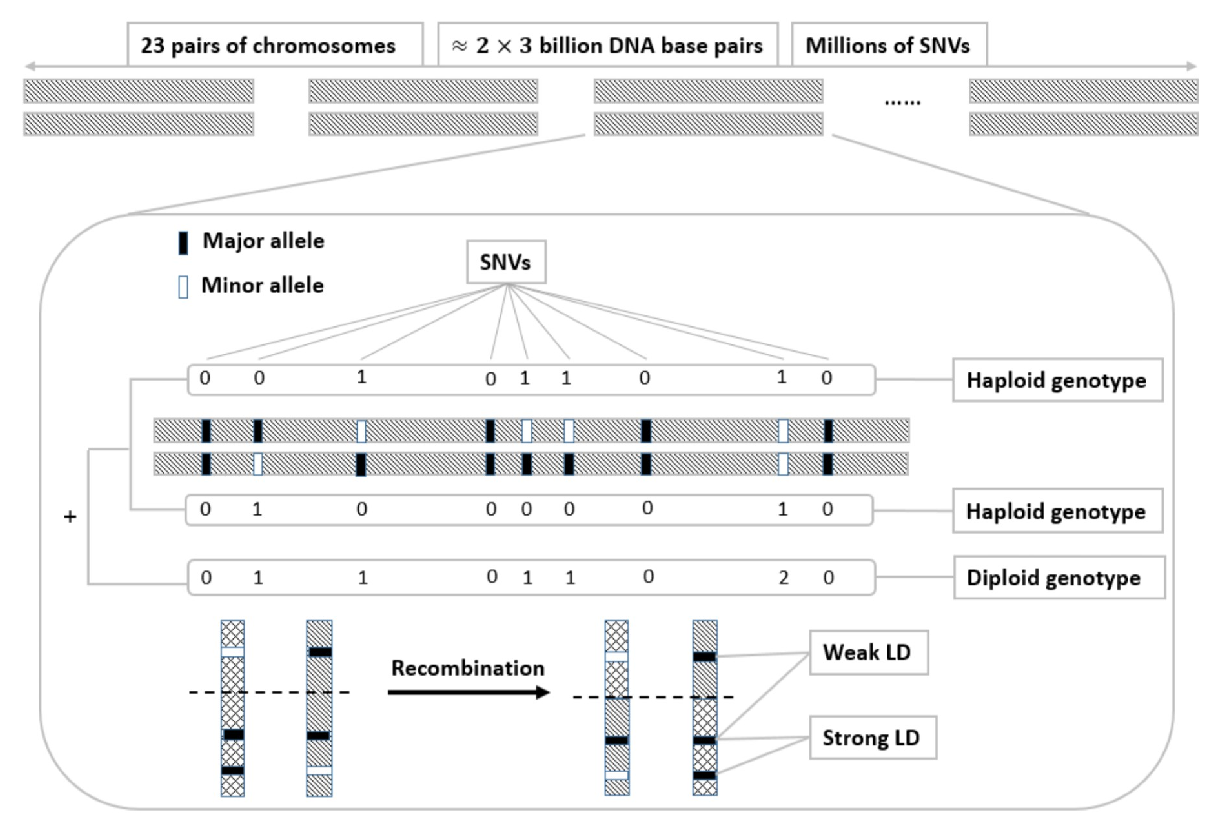
\includegraphics[width = 0.9\linewidth]{./figures/Fig1-human-genomic-overview.eps}
	\caption{人类基因组概览~\cite{samani2015quantifying}
	}
	\label{fig:human-genomic-overview}
\end{figure}

为方便起见,每个SNP位点的三个可能状态(即AA,Aa和aa)分别用0、1和2表示,具体数值取决于每个基因位点上次要等位基因的数量。

连锁不平衡(Linkage disequilibrium,LD)被定义为等位基因在两个或多个位点上的对应关系或非随机关联关系。这种关联关系是遗传机制的结果,即某一个群体有足够的进化时间,基因随机重组的出现将在所有位点产生等位基因的平衡分布。对LD建模的方法有几种,本文中我们主要应用混合建模的LD数据,该建模方法同时考虑了参照基因型数据集和基因重组率的影响。

在遗传过程中,基因重组是一个子过程,在该过程中,一些DNA片段被分离并重新组合,形成新的等位基因组合。基因重组过程产生了所有生物的遗传多样性,基因重组与LD是直接相关的。

\subsection{隐Markov模型}

隐Markov模型(Hidden Markov Model, HMM)~\cite{rabiner1989tutorial,stamp2004revealing}是一种状态不可观测的统计Markov模型,可以通过简单的动态贝叶斯网络表示。具体来说,本章的研究过程中采用了三个假设:(1)~$t$~时刻的状态是由某个状态为~$s_t$~ 隐藏的过程生成的;(2)该过程具有Markov特性;(3)隐藏的状态变量是离散的。
HMM可用于表征诸如相似性、解码和学习等基本问题。 目前,HMM在语音识别~\cite{rabiner1989tutorial}、手写识别~\cite{hu1996hmm}、基因预测~\cite{durbin1998biological}等领域得到了广泛的应用。

本章研究的问题在某种程度上类似于参数学习问题。由于在给定观测或发射序列的推断过程中,所有隐藏状态变量的后验边缘分布都可以通过计算得到,因此我们考虑采用正向-反向算法。

\subsection{卷积神经网络}

卷积神经网络(Convolutional Neural Network, CNN)~\cite{long2017fully,scutti2018what}已成为解决图像分类、分割和回归问题的一种流行方法。但是,尚未发现有应用回归CNN(Regressive Convolutional Neural Network,RCNN)体系结构(其中最后一层是回归层的CNN)来预测基因型序列的研究。与传统的分类分割问题不同,CNN的输出是离散值~\cite{scutti2018what},而RCNN的输出是连续的。

本章针对类似于缺失值预测问题,我们设计了用于单倍型序列预测的RCNN架构。首先,使用公开单倍型数据集来训练和测试所提出的RCNN模型。建立RCNN预测模型后,首先将观测到的二倍体基因序列解析为单倍体,进而推断SNP序列上隐藏SNP的基因型,并将其应用于攻击个体的基因型序列隐私信息。


\section{敌手模型与敌手隐私分析能力度量}\label{sec:adver}

\subsection{敌手模型}

本节提出的敌手模型主要针对现实世界中涉及基因组数据共享的场景。在这种情况下,被攻击对象共享其SNP序列用于研究、医学测试或寻找亲属。由于隐私保护的需求,被攻击者希望隐藏某些可能与遗传病或私人特征有关的敏感SNP。因此,被攻击对象共享其原始SNP序列的变体~$\hat{X}=(\hat{x}_1,\hat{x}_2, ... , \hat{x}_n)$~, 其中~$\hat{x}_i =\{0,1,2\}$~,并隐藏其中某些SNP。假设隐藏的SNP用~$X_h$~表示,可观测的SNP用~$X_O~$~表示,公开的SNP用~$X=(x_1, x_2, ..., x_n)=X_H \cup X_O~$~,其中~$X_i =\{-1,0,1,2\}$~,值~$X_i=-1$~表示~$X_i\in X_h$~是隐藏的SNP。假设已观测被攻击者公开SNP$~X$~序列数据的敌手想要重构原始SNP序列~$\hat{X}$~。为此,敌手可以通过推断攻击获取被攻击者的基因组隐私(例如获得其APOE基因状态~\cite{nyholt2009jim})。要进行这样的推断攻击,敌手将收集一些公开可用的基因组信息~\cite{IGSR2019,howie2014impute2},例如被攻击者所属族群的次要等位基因频率(Minor Allele Frequency,MAF)、LD值、遗传重组率和单倍体基因型参照,如图~\ref{fig:adversary-model} 所示。

\begin{figure}[htbp]
	\centering
	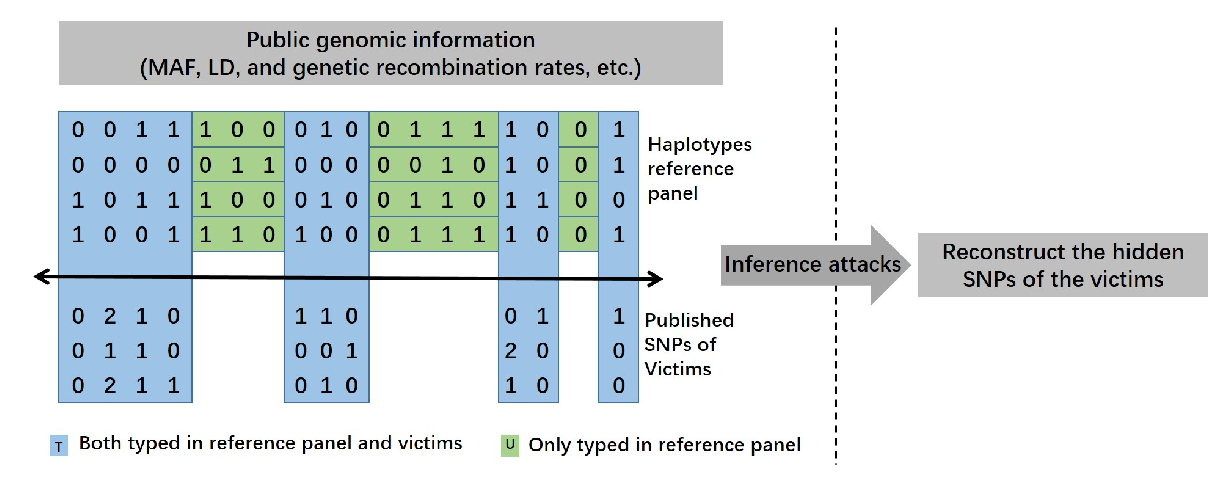
\includegraphics[width = 0.95\linewidth]{./figures/Fig2-adversary-model.eps}
	\caption{基因序列数据属性隐私分析推断敌手模型概览}
	\label{fig:adversary-model}
\end{figure}

假设可访问的公开基因组信息用~${INFOR}_{Pub}$~表示,推断的SNP序列用~$\bar{X}=(\bar{x}_1, \bar{x}_2,...,\bar{x}_n)$~表示。基于基因型隐私的推断攻击的敌手模型~$infer$~可以形式化地表示为
\begin{align}\label{eq:adversary-model}
\bar{X} = infer(X,{INFOR}_{Pub})  
=  infer(X_H,H_O,{INFOR}_{Pub}).
\end{align}

更具体地说,基因序列数据属性隐私推断攻击可以看作是给定已发布的SNP和公开基因组信息,计算每个隐藏SNP的条件边缘概率分布的过程,即
\begin{align}\label{eq:adversary-model-prob}
Prob(X=\{0,1,2\})=Prob(X|(X_O,{INFOR}_{Pub})).
\end{align}
对于每个隐藏SNP位点的隐私数值,其预测值是条件概率最高的那个值。

\subsection{敌手隐私分析能力度量}


为了度量敌手在基因组隐私推断方面的能力,本章使用Ayday等~\cite{ayday2013personal}引入的\textit{基因组隐私度量}方法,从而评估敌手通过推断攻击可以在多大程度上损害被攻击者的基因组隐私。如同Wagner
~\cite{wagner2017evaluating}
所述,有几种不同的基因组隐私度量方法适用于本章的研究。在本章中,假设敌手的目标是隐藏的推断SNP序列的属性隐私值,且仅考虑个体实际拥有的SNP序列,应用\textit{正规不正确性}(即敌手的不正确性),\textit{正规熵}(即敌手的不确定性)和\textit{正规互信息}(即被攻击者的隐私损失)来量化推断攻击模型的隐私分析强度。

作为基因组隐私度量,\textit{正规不正确性}可以表示为
\begin{align}\label{eq:metric-correctness}
E=1- \frac{\sum_1^n \mid \bar{x}_j - \hat{x}_j \mid}  {\mid X_H \mid},
\end{align}
其中~$n$~为被攻击者的SNP数量,~$\bar{x}_j$~为推断出的SNP在~$j$~位点的基因型值,~$\hat{x}_j$~为SNP在~$j$~位点的原始基因型值,~$\mid X_H \mid$~为属于被攻击者隐藏的SNP数量。

尽管不正确性是衡量隐私权的有效指标,但由于被攻击者SNP的原始值未知的,因此在许多场景中该量化指标并不适用。在这些情况下,我们需要其他量化指标来度量隐私。在本章中,我们采用\textit{正规熵}来表示敌手的不确定性,该隐私量化可根据所提出的SNP序列\textit{正规熵}来计算。特别地,
\begin{align}\label{eq:metric-entropy}
H = \frac{\sum_{j=1}^n \frac{H(X_j)}{log(3)}}{\mid X_H \mid},
\end{align}
其中~$H(X_j)= -\sum_{\bar{x}_j=\in \{0,1,2\}}{p(\bar{x}_j)log(p(\bar{x}_j))}$~ 为推断出的SNP在~$j$~位点的熵,~$log(3)$~为~$j$~位点SNP的最大熵,~$\mid X_H \mid$~ 为被攻击者的隐藏SNP数。

该度量指标根据敌手的能力而不是被攻击者的隐私损失来量化敌手在其推断攻击中的置信度。如本文第三章所述互信息可以作为这种度量的基础,为此,我们利用不确定性的递减来表示敌手在推断攻击前后对隐藏SNP序列的不确定性的变化。因此,本章使用正规互信息来量化敌手对被攻击者的平均隐私损失,由于互信息的估计是一个困难性问题,依赖条件概率的分布,故本章利用熵的变化量来估计互信息,即
\begin{align}\label{eq:metric-mutual-information}
I = \frac{\sum_{j=1}^n \frac{H_{MAF}(X_j)}{log(3)}}{\mid X_H \mid}
- H,
\end{align}
其中,~$H_{MAF}(X_j) = -\sum_{x_j=\in \{0,1,2\}}{p_{MAF}(x_j)log(p_{MAF}(x_j))}$~ 表示SNP在~$j$~位点的自然熵,~$p_{MAF}(x_j)$~为根据MAF数据集SNP发生的概率。公式~\ref{eq:metric-mutual-information} 中定义的度量表示推断攻击引起的熵变化量,从而可以度量推断攻击的强度,它还可以评估被攻击者在推断攻击时的基因组隐私损失。

\section{独立序列型数据隐私分析推断方法}\label{sec:infer}

在这一节中,对于所使用的敌手模型,我们提出了两种推断攻击策略,一个是基于改进的HMM (iHMM)的隐私推断方法,另一个是基于RCNN模型的隐私推断方法。

\subsection{基于iHMM的隐私分析}

为了提高基因组隐私推断的性能,本节方法不同于文献~\cite{samani2015quantifying}中那样直接推断被攻击者的隐藏的SNP基因型,而是受IMPUTE2 ~\cite{howie2009flexible}基因型插补方法的启发,我们将
隐私分析攻击过程分为三个步骤:(1) 使用Markov链Monte Carlo抽样策略将观测到的被攻击者的SNP序列分阶段转为单倍型;(2) 使用HMM模型分别推断每个被攻击者的隐藏单倍型基因型数值;(3)结合对每个被攻击者推断的单倍型结果,形成推断的基因型序列。


在模型的详细构建中,我们将参照数据集和被攻击者的SNP序列分为~$T$~(同时出现在参照数据集和被攻击者中的SNP序列)和~$u~$(不出现在被攻击者中,但出现在参照数据集中的SNP序列)。我们假设有~$n$~个被攻击者, ~$H_R^T$~表示~$T$~中SNP序列的参照单倍型集合,~$H_V^T$~表示被攻击者在~$T$~中观察到的SNP序列的单倍型集合,~$H_V^U$~表示与~$U$~中SNP序列相对应的被攻击者隐藏的单倍型集合,~$H_V^T=\{H_{V,1}^T,H_{V,2}^T,..., H_{V,n}^T\}$~表示~$T$~中与SNP序列对应的被攻击者单倍型,其中~$H_{V,i}^T$~表示第~$i$~个被攻击者的单倍型,~$\rho~$~表示群组基因重组映射率。

更具体地说,基于iHMM的推断攻击可以分三个步骤进行,详细说明如下:
\begin{enumerate}
	\item[(1)] 敌手根据观测到的被攻击者的基因型数据,随机产生~$H_V^T$~的单倍型。然后,敌手通过多轮Markov链Monte Carlo迭代更新~$H_V^T$~中的单倍型。在每次迭代中,敌手通过从~$p(H_{V,i}^T|G_{V,i}^T,H_{V,-i}^T,H_R^T,\rho)$~中抽样来更新第~$i$~个被攻击者的阶段性单倍型对~$H_{V,i}^T$~。
	\item[(2)] 敌手通过基因重组模型利用HMM模型推断~$H_V^u$~中的单倍型。在每次迭代中,敌手根据条件概率分布~$p(H_{V,i}^U|H_{V,i}^T, H_R^{T \cup U},\rho)$~推断第~$i$~个被攻击者对应~$U$~中的SNP序列的隐藏单倍型对~$H_{V,i}^u$~。 
	\item[(3)] 敌手把对每个被攻击者推断出来的单倍型对组合起来,得到被攻击者隐藏的SNP序列的推断基因型。
\end{enumerate}

在步骤(1)中每次迭代的分阶段步骤中,抽样条件为~$k$~个最接近的单倍型,其结果由其到第~$i$~个被攻击者的汉明距离确定。基于基因重组过程,利用HMM模型来推断计算条件分布,采用Monte Carlo方法重构基因解析空间。因为推断得到的状态空间包含~$H_R^T$~中单倍型的所有状态和~$H_{V,-i}^T$~中当前猜测的单倍型,所以可以获得更多隐私关联信息。

在步骤(2)中,HMM状态空间包含了所有参照单倍型~$H_R^{T \cup U}$~,此步骤类似于文献~\cite{samani2015quantifying}中基于基因重组模型的过程,该模型受文献~\cite{marchini2007newa}的启发。然而,我们推断每个被攻击者的单倍型数值,而不是直接推断基因型数值。

步骤(1)至(3)中描述的攻击策略与文献~\cite{samani2015quantifying}中描述的攻击策略不同,后者直接推断隐藏SNP的基因型值。在本章中,敌手结合了Markov链Monte Carlo抽样和HMM推断技术,提高了目标SNP序列的条件分布所获得的隐私分析效果。

\subsection{基于RCNN的隐私分析}

基于RCNN的攻击也分为三个步骤,步骤(1)和(3)与基于iHMM的隐私分析推断攻击是相同的,只有步骤(2)不同。同样地,敌手观测公开基因组信息和被攻击者SNP序列,将基因型分为单倍型,分别推断出隐藏的单倍型对,然后将推断出的单倍型对组合成基因型。在这里,我们将基于RCNN攻击的步骤(2)做说明如下。

我们构造基于RCNN的基因序列属性隐私分析目标模型为
\begin{align}\label{eq:rcnn}
H_{V,i}^U  \leftarrow RCNN(H_{V,i}^T, H_R^{T \cup U}),
\end{align}
其中,给定一个参照单倍型集和一个基于观察到的SNP序列的相位单倍型集,公式~\ref{eq:rcnn}的目标是推断这些隐藏部分的值(即0或1)。由于被攻击者的公开参照单倍型和观察到的SNP序列都属于同一群体(如CEU或CHS~\cite{igsr2015which}),因此这些数据具有相同的特征,可以通过神经网络进行分析。

我们对参照数据~$H_R^{T \cup U}$~提出了一个RCNN模型,将这些数据分成两组:一组是训练集~$H_{Rtrain}^{T \cup U}$~,另一组是测试集~$H_{Rtest}^{T \cup U}$~。然后对最小值~$min(\|H_{Rtest}^{ U} - \hat{H}_{Rtest}^{U}\|)$~目标选择最佳的训练网络,其中~$\hat{H}_{Rtest}^{U}$~ 表示测试集的预测值。敌手可以使用这个优化的网络来推断被攻击者单倍型的隐藏值,具体过程如图~\ref{fig:rcnn_infer} 所示。

\begin{figure}[htbp]
	\centering
	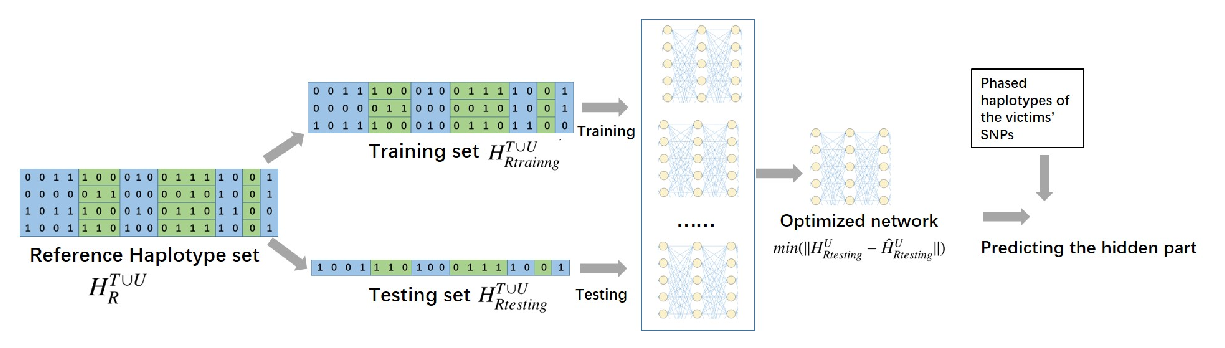
\includegraphics[width=0.95\linewidth]{./figures/Fig3-RCNN-inference-attack.eps}\\
	\caption{基于RCNN的隐私分析模型}
	\label{fig:rcnn_infer}
\end{figure}


\begin{figure}[htbp]
	\centering
	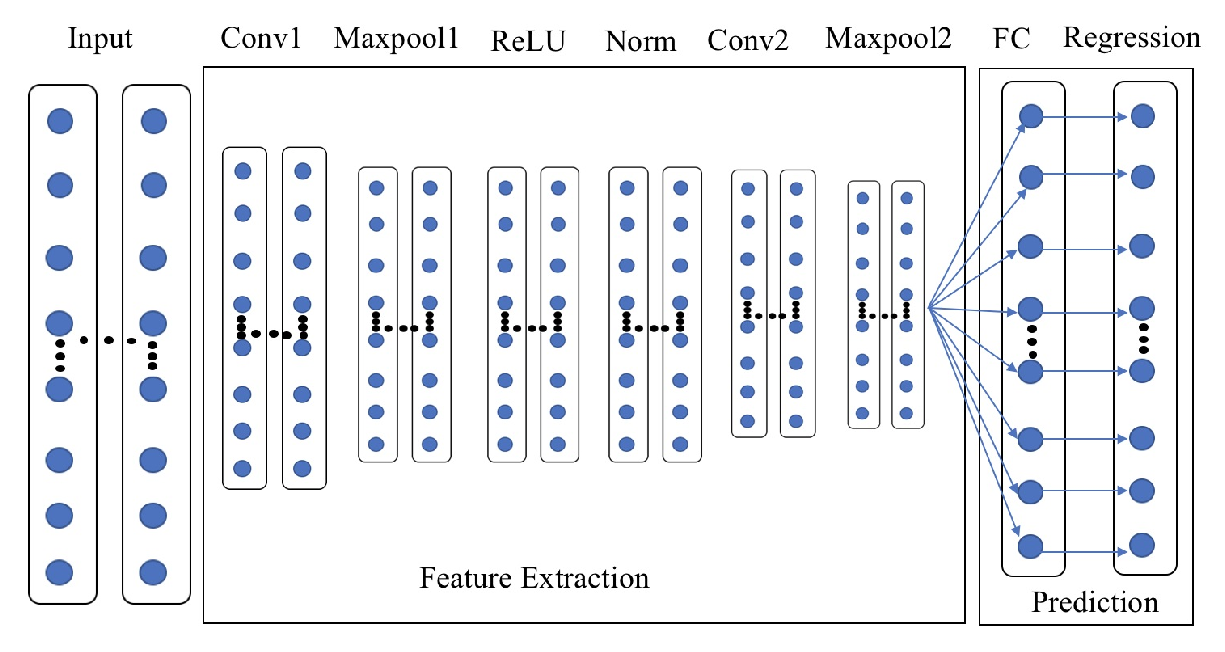
\includegraphics[width=0.7\linewidth]{./figures/Fig4-RCNN-structure.eps}\\
	\caption{基于RCNN的基因隐私分析过程}
	\label{fig:RCNN}
\end{figure}
基于RCNN的基因隐私分析过程如图~\ref{fig:RCNN}所示(其中,Conv为卷积层,NA为正规化层,FC为完全联通层),该过程包含8层网络,输入由观测到的SNP序列的单倍型组成,最后一层回归层生成隐藏SNP序列的单倍体型值。最后一层是代表隐藏SNP序列的单倍型的回归层。在训练阶段,RCNN能够提取基因型的影响因子,检验均方误差(Mean Squre Error,MSE)是否收敛。利用RCNN训练得到的分类器,可以对测试数据集中的隐藏SNP序列的单倍型值进行推断。

该网络可实现两项主要任务:特征提取和预测。该网络包括八层,两个卷积层(Conv1和Conv2)、两个最大池层(Maxpool1和Maxpool2)、一个整流线性单元层(ReLU)和一个归一化层(Norm),ReLU层减少了训练所需的时间周期,但是其错误率比传统的双曲正切更高。规范层提高了通用性,降低了错误率。值得注意的是,ReLU层和Norm层并不会改变特征映射的大小。池化层汇总了相邻池化单元的输出。预测步骤完全由连接(FC)层和回归层执行。输入层由~$8\times 1$~个影响因子组成(1个月) ,Conv1和Conv2各自的过滤器大小(~$F$~)为~$1\times 1$~ ,并且过滤器的数量(~$N$~)为25,填充大小(~$P$~)为0,Maxpool1和Maxpool2的步长(~$S$~)为~$2\times 2$~。因此,在每个max池层之后,特征图的维数除以2。


为训练RCNN模型,我们最小化损失函数,使用均方误差(MSE)作为损失函数,其定义为
\begin{equation}
\text{Loss}=\frac{1}{N}\sum_{i=1}^{N}|d_{t}^{i}-d_{o}^{i}|^{2},
\end{equation}
其中~$n$~是数据集中的条目数,下标~$i$~表示数据集中的第~$i$~个点位。


如图~\ref{fig:RCNN}所示,一旦在Maxpool2层中提取了额外的特征,我们就可以将其连接到FC层,并将所有的特征压缩成一个维度。在训练过程中,如果在当前迭代次数未达到期望的MSE,则训练将继续进行,直到达到最大的迭代次数或所期望的MSE。如果达到最大迭代次数,则无论MSE值如何,训练过程都会停止。为了验证该方法的可行性和实用性,将测试数据集输入训练好的RCNN模型中,并利用该模型预测隐藏SNP序列的单倍型,从而对总体性能进行评估。


\section{实验与分析}\label{sec:resul}
在本节中,将根据各种指标评估本章提出的序列型数据属性隐私分析推断攻击方法的性能,并基于实验所得到的结果与之前的工作进行比较。

\subsection{数据集选取}
实验选取了来自HapMap项目~\cite{thorisson2005international}第三期的数据集,该数据集在互联网上是公开的。在这个项目中,从世界各地11个不同族群中收集匿名的基因组数据用于基因研究。在不失一般性的前提下,本章采用了2010年5月发布的北欧和西欧祖先(CEU)族群22号染色体的数据集。该数据集包含了个体的单倍型序列,并且还包括了这些群体的MAF、成对LD值和基因重组率。我们将这些数据视为公开背景数据。此外,HapMap项目数据集中也包含165个个体的基因型序列。本章将使用这些数据作为选择的无关亲属的基因组数据,同时这个数据集也在文献~\cite{samani2015quantifying}中使用过。
\subsection{实验结果对比与分析}

在本节的实验中,随机隐藏被攻击者SNP序列的不同百分比(从5\%到60\%),使用所提出的攻击模型推断隐藏的SNP序列,并根据第~\ref{sec:adver}节中所描述的三个隐私度量指标来量化基因组隐私试验结果。

首先,随机隐藏10\%的被攻击者的SNP,并使用不同的攻击模型评估敌手的隐私分析推断能力。然后,进行20次实验,取每个量化指标结果的平均值。对基于iHMM和RCNN模型的隐私分析推断攻击强度进行量化计算,敌手的不正确性、敌手的不确定性和被攻击者的隐私损失结果如表~\ref{tab:performance-10per}所示。在此表中,M1-LD,M2和RM分别表示文献~\cite{samani2015quantifying} 中基于一阶Markov链(利用公开二元LD数据),二阶Markov链和基因重组模型的推断攻击,而iHMM和RCNN分别表示基于iHMM和RCNN模型的基因序列属性隐私推断攻击。在错误率列中比较了不同推断攻击的不正确性,本章提出的两种方法结果都显示出在不正确性指标上明显降低,与RM方法相比,iHMM的性能更好,而RCNN的性能稍差。因为文献~\cite{samani2015quantifying} 中的作者在其论文中没有考虑不确定性和隐私损失的度量,所以本节根据计算这两个度量的需要,对其实验进行了改进。结果表明,这两种度量方法同样适用于基因组隐私的度量,在表~\ref{tab:performance-10per}的正规熵列和正规隐私损失列中分别显示了不确定性和隐私损失方面的性能结果。结果表明,利用基于iHMM的推断攻击,敌手可以获得较低的不确定性,并获得更多被攻击者的隐私信息。

为了进一步支撑比较结果,并与文献~\cite{samani2015quantifying}中提出的实验保持一致,本节进行了另一个含有40\%隐藏SNP序列的实验。试验结果如表~\ref{tab:performance-40per}所示,结果表明与表~\ref{tab:performance-10per}中的结论一致,本章所提出的独立基因序列数据隐私分析方法能够在各种指标对比下获得更好的优势。

\begin{table}[htbp]
	\caption{当10\%SNP序列被隐藏时,不同基因隐私分析推断效果对比}
	\label{tab:performance-10per}
	\begin{tabular}{lccc}
		\hline
		& Error rate & Normalized entropy & Normalized privacy loss\\
		\hline
		M1-LD (Samani et al.) & 0.3356  & 0.4872 & 0.1864 \\
		M2 (Samani et al.)    & 0.2400  & 0.3419 & 0.3316\\
		RM (Samani et al.)    &  0.0578 & 0.069 & 0.6046 \\
		iHMM (Ours)          & 0.0085  &0.0295 & 0.6520 \\
		RCNN (Ours)          & 0.0753  &0.0973 & 0.5143\\
		\hline
	\end{tabular}
\end{table}


\begin{table}[htbp]
	\caption{当40\%SNP序列被隐藏时,不同基因隐私分析推断效果对比}
	\label{tab:performance-40per}
	\begin{tabular}{lccc}
		\hline
		& Error rate & Normalized entropy & Normalized privacy loss \\
		\hline
		M1-LD (Samani et al.) & 0.3623 & 0.4867 & 0.1873 \\
		M2 (Samani et al.)    & 0.2873 & 0.3489 & 0.3251 \\
		RM (Samani et al.)    & 0.0923 & 0.0902 & 0.5838 \\
		iHMM (Ours)          & 0.0136 & 0.0430 & 0.6342 \\
		RCNN (Ours)          & 0.1028 & 0.1345 & 0.5347\\
		\hline
	\end{tabular}
\end{table}

\begin{figure}[htbp]
	\centering
	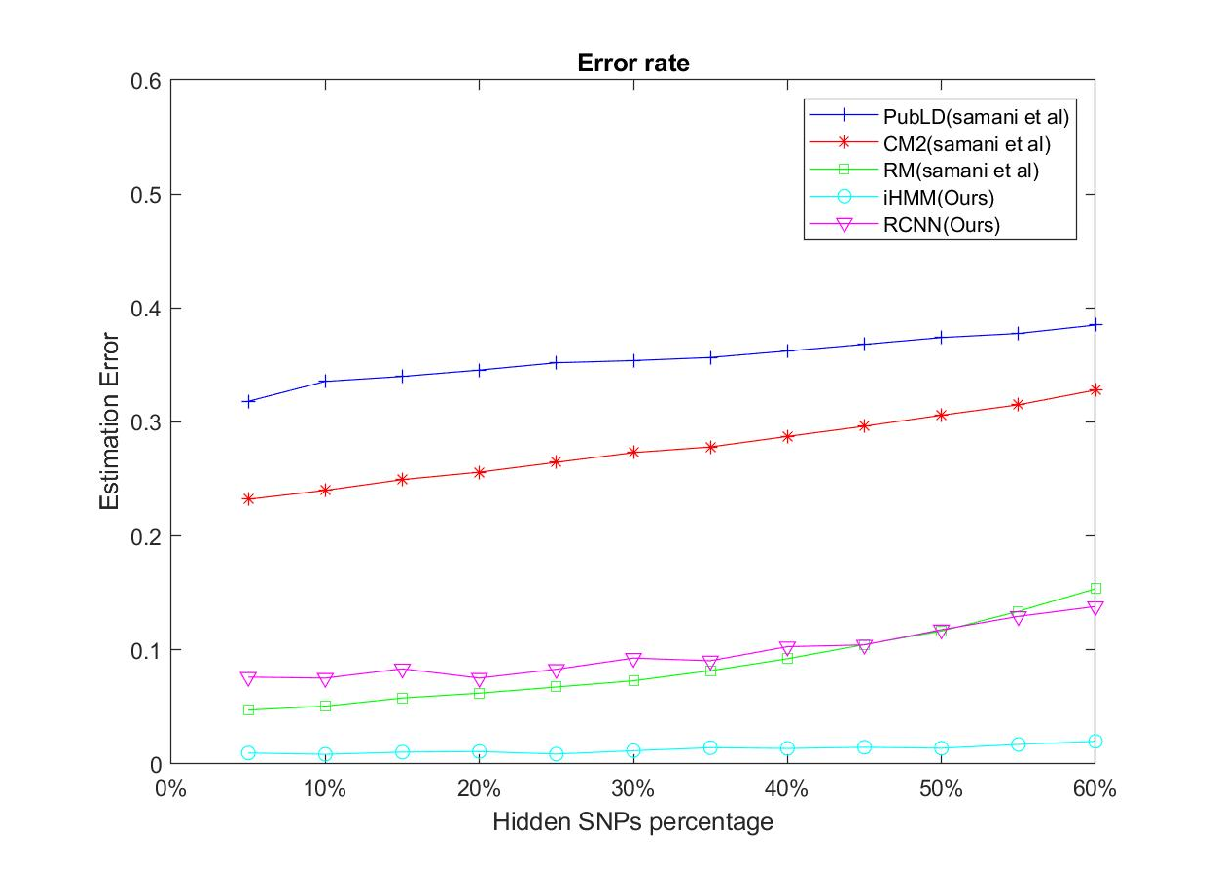
\includegraphics[width =0.8\linewidth]{./figures/Fig5-genomic-privacy-quantifying-incorrectness.eps}
	\caption{不同基因隐私分析模型的基因组隐私敌手错误率对比}
	\label{fig:error}
\end{figure}
\begin{figure}[htbp]
	\centering
	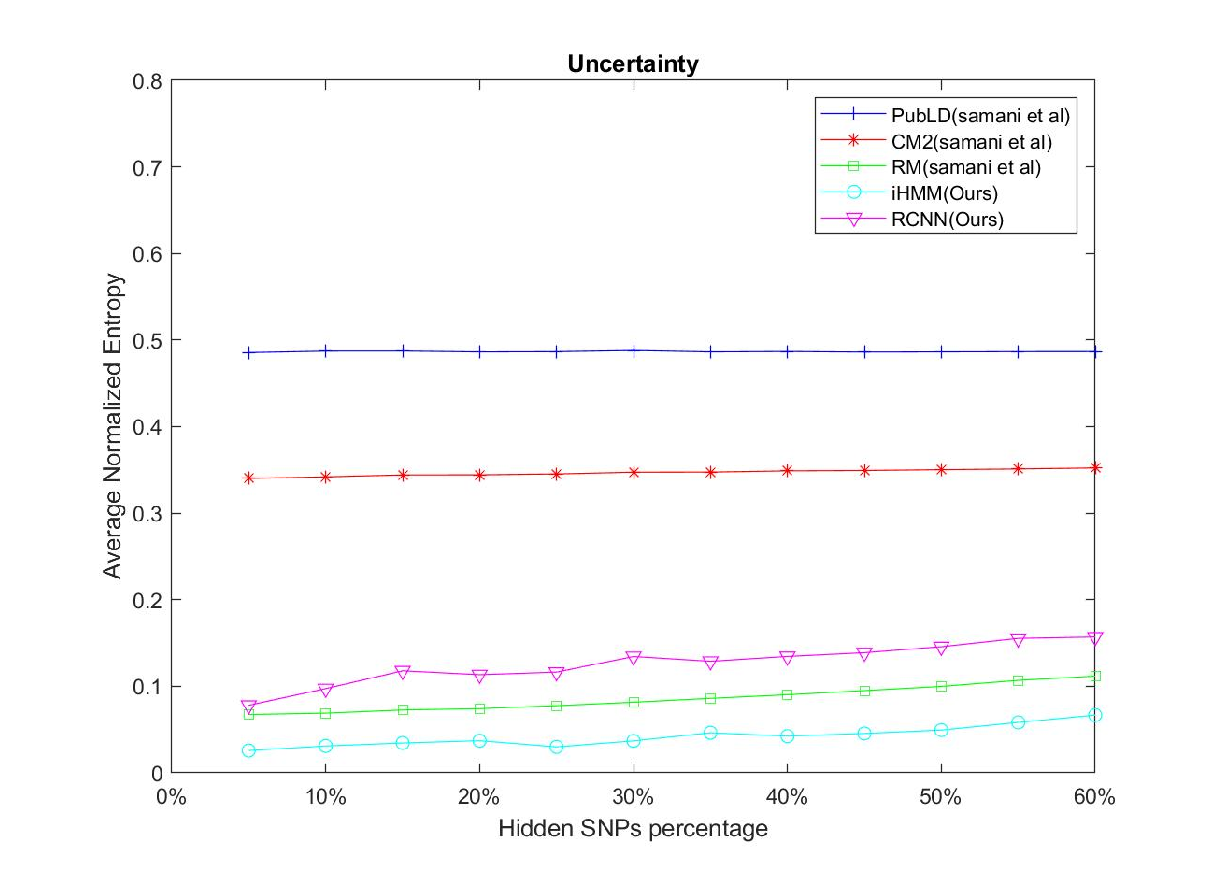
\includegraphics[width =0.8\linewidth]{./figures/Fig6-genomic-privacy-quantifying-uncertainty.eps}
	\caption{不同基因隐私分析模型的基因组隐私敌手不确定度对比}
	\label{fig:uncertainty}
\end{figure}
\begin{figure}[htbp]
	\centering
	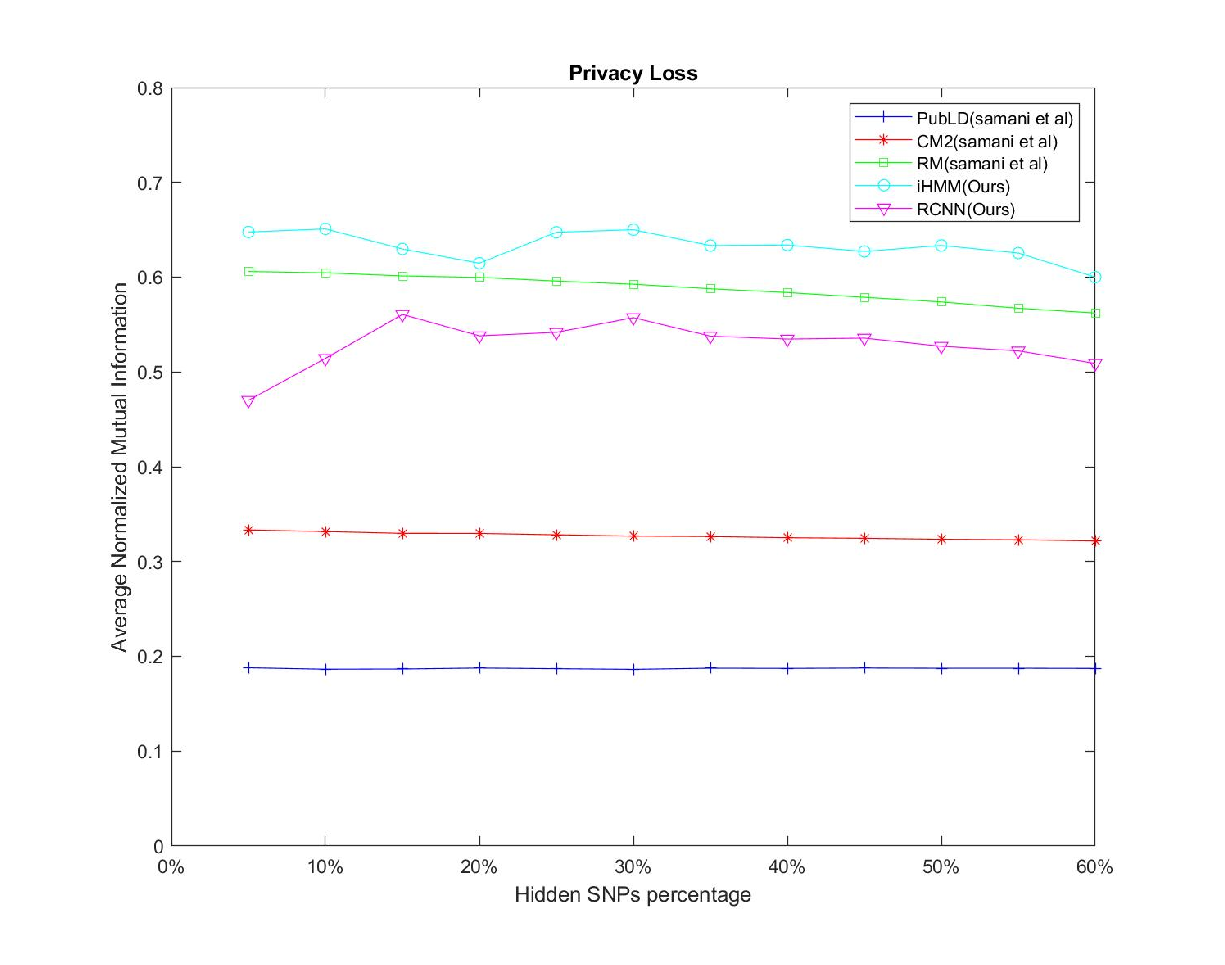
\includegraphics[width =0.8\linewidth]{./figures/Fig7-genomic-privacy-quantifying-privacyloss.eps}
	\caption{不同基因隐私分析模型的基因组隐私敌手隐私获取量对比}
	\label{fig:privacyloss}
\end{figure}

然后,为了观察隐藏SNP序列数量对不同推断攻击的影响,本节又进行了一组实验,实验中使用了不同比例(5\% - 60\%)的隐藏SNP序列对基于LD、2阶Markov链、重组模型、iHMM和RCNN等不同模型的基因序列数据隐私分析模型进行测试。敌手的不正确性、敌手的不确定性和敌手的基因组隐私损失结果分别如图~\ref{fig:error}、图~\ref{fig:uncertainty}和图~\ref{fig:privacyloss}所示。

在图~\ref{fig:error}中,根据敌手的不正确性展示了基于不同模型的基因隐私推断攻击结果。当被攻击者少量的SNP序列被隐藏时,可以发现这些攻击的推断能力会增加(即,被攻击者的SNP序列暴露给敌手的越多,不正确性越低)。与之前的工作相比所提出的两种攻击模型在不正确性方面均显示出更好的推断能力。当隐藏更多SNP序列(大于50\%)时,基于RCNN的攻击性能优于基于重组模型的攻击;当隐藏更少SNP序列时(小于45\%)时,基于重组模型的攻击性能略差。

在图~\ref{fig:uncertainty}中,根据敌手的不确定性显示了基于不同模型的推断攻击的结果。可以看出,当被敌手隐藏的SNP序列越少时,这些攻击的推断能力越强(即,被攻击者的SNP序列暴露给敌手的越多,不确定性越低),结果与图~\ref{fig:error}的结果一致。对比表明,基于iHMM的攻击总是比其他攻击效果更好,而基于RCNN的攻击效果并非始终都是好的。

同样的,在图~\ref{fig:privacyloss}中的结果可以看到被攻击者隐私损失的结果。同样,当被攻击者隐藏的SNP越少,这些攻击的推断能力就越强(即被攻击者的SNP序列暴露给敌手的越多,隐私损失越大)。

\section{小结}\label{sec:concl}

本章针对独立基因序列数据共享场景,提出了两种针对序列型基因数据的隐私分析攻击方法,通过改进的隐Markov模型或回归卷积神经网络模型,利用网络公开基因组信息和个体的部分公开共享SNP序列数据推断个体的隐私基因型信息。研究表明,敌手能够准确、低不确定性和高隐私损失地推断出个体的私有隐藏SNP隐私信息。实验表明,所提出的攻击扩展并显著改进了现有的工作。通过基于公开的基因组数据对个体基因组隐私进行量化,本章的工作可以帮助人们更好地理解当前基因组隐私面临的风险,促进隐私领域更加小心地应用基因组数据,促进研究人员设计更好的隐私保护模型(如后文研究的基于风险访问控制模型)以适应性地保护基因序列数据隐私。

%风险访问控制
\chapter{关联序列型数据属性隐私推断模型}
\label{chap:inference-attack-on-related-sequenced-data}
\textit{ }

\textit{随着不同机构和个人更加容易获取基因组数据,且这些敏感数据被广泛应用于医疗、保险、寻亲及社交等场景,对基因数据安全和隐私的担忧也在不断加剧。最近一些实际攻击和真实事件更加增强了对基因组隐私的担忧。为了证实并披露在序列型数据属性隐私方面,个人共享基因数据也会大量泄漏他人属性隐私的机理。本章针对关联基因序列数据共享会造成的隐私泄露问题展开研究,并证实了上述问题会变得更严峻。本章中,利用因子图和置信传播算法针对亲属间的基因序列属性隐私建立分析推断敌手模型和分析算法,提高亲属基因组属性隐私推断攻击的效果。该模型考虑了单核苷酸多态性间高阶相关性,利用公开DNA参照数据集和全基因组关联研究(GWAS)目录数据,提高了推断攻击模型的属性隐私分析强度。该模型的敌手隐私分析强度通过第\ref{chap:entropy-metric-model}章所提出的隐私度量框架,将隐私损失量作为评价指标进行了量化。实验结果表明,所提出的攻击更适合于高密度基因组数据隐私推断,且具更低不正确性和不确定性,以及更多隐私损失,显著提高了基因序列属性隐私推断攻击能力。}

\section{概述}
得益于生物技术的快速发展,人们可以廉价地对DNA进行测序,并很容易地将自己的基因组数据分享给他人。越来越多的人为了不同的目的(如精准基因组医学、全球基因组研究、了解个人遗传疾病情况、寻找祖先和亲属或者仅仅为了娱乐),将其基因组数据共享。政府、研究机构、医疗组织、健康相关网站和在线社交网络已收集了成千上万个人基因组数据,其中大部分数据都可以下载或在网上公开共享。

尽管网上的大部分基因组数据都是匿名化的,但是这些数据都可以被去匿名化重新识别~\cite{greenbaum2008genomic,humbert2015de}。即使一个个体在共享其基因组数据之前隐藏了部分数据,也能重构隐藏部分的基因序列数据,并推测获知其私人疾病和特征信息。因此,共享基因组数据的所有者可能面临来自雇主或保险公司的歧视风险。此外,超过99.9\%的基因组数据对人类来说是相同的,在亲属中具有相同基因组数据的占比比例更高。因此,若一个人暴露了其基因组数据,就会导致其基因组隐私和其亲属的基因组隐私受到威胁,如亲属关系隐私和家族身份隐私~\cite{rohlfs2012familial}。


实际情况会更糟,最近的新闻报道称,美国警方通过开源遗传数据库中的家族成员基因组数据,发现并逮捕了金州杀手,该罪犯在1974年至1986年期间在加州造成12人死亡和至少50起强奸案。这一消息引起了人们对基因隐私的极大关注。若有亲属参与了基因研究或在网上分享了他们自己基因,你应该担心自己的隐私吗?是否有可能从某人的亲属基因数据中重构该人的基因组数据?通过这种方式可以重构多少基因信息?通过亲属的基因数据可以泄露该人的多少基因隐私?

基于最近的研究和真实的新闻报道,本文针对相互关联序列型数据的属性隐私提出了一种敌手模型和概率推断方法。该模型是针对亲属基因组隐私的高精度推断攻击,并利用第\ref{chap:entropy-metric-model}章提出的度量方法对基因隐私和隐私推断攻击强度进行了量化。该攻击模型旨在从公开的基因组数据和网站上的亲属基因组信息中推断出个人的基因组属性隐私信息。提出了一个统一的关联基因序列属性隐私推断敌手模型,提出了一个基于离散隐Markov模型、高密度参考数据集和GWAS目录的推断攻击方法,并利用因子图和置信传播算法实现了基因属性隐私推断攻击。与Humbert等~\cite{humbert2013addressing,humbert2017quantifying}和Deznabi等~\cite{deznabi2018inference}的工作相比,我们的贡献是:

\begin{enumerate}
	\item 提出了一种利用9种公开的和观测到的家庭成员基因组数据进行推断攻击的敌手模型,攻击者的目标是推断被攻击者的基因组属性值。
	\item 提出了利用高密度参照数据集IMPUTE2~\cite{howie2014impute2}中SNP序列的相关性进行基因序列属性隐私推断攻击,并设计了一个基于因子图和置信传播模型的基因属性隐私推断攻击算法。
	\item 利用互信息度量所提出的基因序列隐私属性推断攻击强度,量化基因组隐私泄露量,并刻画了攻击者对属性隐私不确定性的降低和被攻击者基因属性隐私损失的增加。
	\item 针对被攻击者的基因属性隐私推断,得到了非常高的准确性和更低的不确定,比以前的工作更加适用于高密度基因组数据隐私分析。
\end{enumerate}

\section{相关背景知识}
\label{sec:backgrounds}
在本节中,我们简要介绍遗传学的背景和基于因子图的置信传播。

\subsection{基因组信息}

人类基因组被编码为23个染色体对中的DNA,并包含约30亿个核苷酸对。 每个染色体都是双螺旋结构,由两个互补的核苷酸核苷酸(A,T,C或G)聚合链组成。人类 99\% 的DNA信息是一样的,仅有0.5\% 的基因组信息存在显著差异。当基因组序列中的单个核苷酸 (A,T,C或G) 在遗传过程中发生变化时,DNA序列产生变异。

单核苷酸多态性 (Single-Nucleotide Polymorphism,SNP)是在基因组中特定位置出现的单个核苷酸变体,其中每个变体在种群中都以一定程度的概率存在。 对于每个SNP,存在三种可能的基因型:(i) 普通等位基因是纯合子, (ii) 对于较不常见的等位基因是杂合的,(iii) 稀有等位基因纯合子; 通常分别编码为0、1和2。 SNP经常与疾病和个人特征有关, SNPedia和GWAS Central是支持全基因组关联研究 (GWAS) 中的个人基因组注释、解释和分析的数据库。

孟德尔遗传定律表明一个人的SNP都是是独立于其父母继承的。 对于一个SNP位点,一个等位基因来自父亲,一个等位基因来自母亲,概率为0.5。 本章工作依照文献~\cite{humbert2013addressing}和~\cite{deznabi2018inference}中的模型使用该定律,参见图~\ref{fig:Mendelian-law}中的概率模型。

\begin{figure}[htbp]
	\centering
	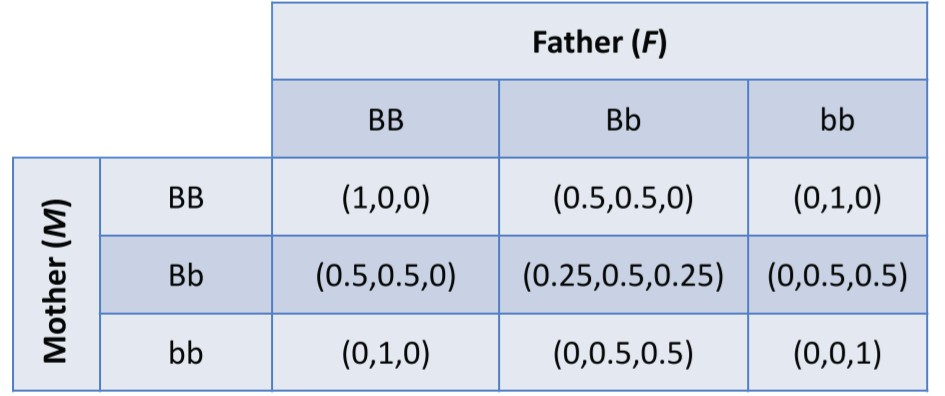
\includegraphics[width=0.6\linewidth]{./figures/Mendelian-law.jpg}
	\centering
	\caption{SNP孟德尔遗传定律概率模型}\label{fig:Mendelian-law}
\end{figure}

连锁不平衡(Linkage Disequilibrium,LD)由两个或多个基因座上等位基因的对应关系或非随机关系定义。 研究人员提出了各种方法来描述SNP之间的相关性,有三种广泛应用的方法,分别使用公开的等位基因频率和连锁不平衡、基因型数据集和遗传重组率~\cite{samani2015quantifying} 。IMPUTE2~\cite{howie2014impute2}是一种缺失基因型的概率估算方法,其通过使用高密度单倍型参照数据集、遗传重组率、离散隐Markov链模型和Markov链Monte Carlo采样策略而提出。 与在文献~\cite{humbert2013addressing,humbert2017quantifying}中使用的成对连锁不平衡和在文献~\cite{deznabi2018inference} 中使用的简单(隐藏) Markov链不同,在本章工作中使用IMPUTE2中的方法作为基因属性隐私分析推测的关联性计算和采样算法。

\subsection{置信传播}

置信传播~\cite{kschischang2001factor} 是一种用于在图结构模型上进行推断的消息传递算法,且在贝叶斯网络和Markov随机域上运行效果较好。 其在观测到的节点上以条件概率的方式计算未观测到的节点的边缘概率分布。 置信传播在具有近似结果的循环因子图和具有精确结果的无循环因子图上均具有良好的性能。 置信传播在人工智能和信息论中被广泛使用。 在本章中,使用 SumProductLab作为基本开发工具来实现针对所提出的基因序列属性隐私推断攻击的置信传播算法。

\section{关联基因序列数据隐私分析敌手模型}
\subsection{数据模型}
对于特定的家庭,有~$n$~个家庭成员 ~$S=\{s_1,s_2,...,s_n\}$~,以及该家庭的亲属结构图 ~$T=\{S,R\}$~ ,其中 ~$S$~ (是家庭成员的集合) 赋予为 ~$T$~ 的顶点,而 ~$R$~ (是家庭成员关系的集合,若 ~$s_i$~ 是 ~$s_j$~ 的父母,则 ~$r_{i,j}=1$~) 赋予为 ~$T$~ 的边。 假设一个人的SNP集为 ~$\mathbf{x}=(x_1,x_2,...,x_m)$~ 并具有 ~$m$~ 个SNP,其中 ~$x_i \in \{0,1,2\}$~(特定的SNP ~$X_I$~ 具有 ~$"BB"$~,~$"Bb"$~ 和 ~$"bb"$~ 的基因型,可以分别用0、1和2来赋值),因此 ~$s_i$~ 的SNP集可以赋予为 ~$\mathbf{x}_i=(x_{i,1},x_{i,2},...,x_{i,m})$~。令矩阵 ~$\mathbf{X}$~代表整个家族的所有SNP,则

\begin{equation}
\mathbf{X}=
\left[
\begin{matrix}
x_{1,1} & x_{1,2} & ...    & x_{1,m} \\
x_{2,1} & x_{2,2} & ...    & x_{2,m} \\
\vdots  & \ldots  & \ldots & \vdots  \\
x_{n,1} & x_{n,2} & ...    & x_{n,m}
\end{matrix}
\right]
\end{equation}

对于某个族群的某个人,如 CEU~\cite{auton2015a},一个SNP的概率分布由等位基因频率决定。  因此,某个族群中任意人的SNP ~$x_i \in \mathbf{x}$~ 服从该等位基因座的等位基因分布 ~$\mathbf{p}_i$~ ,其中 ~$\mathbf{p}_i=\{p_{i,0},p_{i,1}, p_{i,2}\}$~, ~$p_{i,0}+p_{i,1}+p_{i,2}=1$~。然后设任意个体的SNP序列为 ~$\mathbf{x}$~, 有

\begin{equation}
\left(
\begin{matrix}
x_1          & x_2 & ... & x_m \\
\mathbf{p}_1 & \mathbf{p}_2 & ... & \mathbf{p}_m
\end{matrix}
\right)
\end{equation}

由于减数有丝分裂和DNA重组,一个人的SNP之间存在某些关联关系,其中成对的连锁不平衡是SNP最常见和最基本的关系, 若 ~$x_i$~ 和 ~$x_j$~ 相互关联,则存在系数 ~$f_{i,j}$~ 。基于成对连锁不平衡,可以通过总体SNP集合来训练得到其他高阶关联关系。

此外,一个人的SNP决定了其自己的外在特征和疾病。 设 ~$\mathbf{t}$~ 为可观测到的性状, ~$\mathbf{d}$~ 为与基因组有关的疾病。  性状 ~$T_i \in \mathbf{t}$~ 的表型与子集 ~$\mathbf{x}t_i \subseteq \mathbf{x}$~ 有关, 疾病 ~$D_i \in \mathbf{d}$~ 与子集 ~$\mathbf{x}d_i \subseteq \mathbf{x}$~ 有关。 人类表型本体论项目(Human Phenotype Ontology project)~\cite{koehler2014human}和GWAS目录( GWAS Catalog)~\cite{macarthur2017the}中发布了唯一的SNP特征和SNP疾病关联关系数据。


在实际中,往往部分数据已知而部分数据未知。SNP序列数据是敏感的隐私数据,人们总是在共享或发布基因组数据之前隐藏一些SNP或在SNP中添加噪音。 加噪的方式会使基因组数据杂乱而导致医学研究和精准医疗得到难以预料的结果,因此人们通常只是隐藏了不想共享的部分SNP序列取值。 因此,家族成员的已知SNP赋为 ~$\mathbf{X}_K$~, 未知SNP赋为 ~$\mathbf{X}_u$~,其中 ~$\mathbf{X}_K \perp\mathbf{X}_U$~ 和 ~$\mathbf{X}_K \cup \mathbf{X}_U = \mathbf{X}$~;家庭成员的已知特征是 ~$\mathbf{T}_k$~,未知特征是 ~$\mathbf{T}_u$~;家庭成员的已知基因组疾病是 ~$\mathbf{D}_k$~, 未知基因组疾病是 ~$\mathbf{D}_U$~。同样,~$\mathbf{T}_K \perp \mathbf{T}_U$~,~$\mathbf{D}_K \perp \mathbf{D}_U$~, ~$\mathbf{T}_K \cup \mathbf{T}_U = \mathbf{T}$~,以及 ~$\mathbf{D}_K \cup \mathbf{D}_U = \mathbf{D}$~,其中 ~$\mathbf{T}$~ 表示家庭成员的可观测基因组特征,~$\mathbf{D}$~ 表示家庭成员的遗传疾病。 ~$\mathcal{F}_T(x_i^F,x_i^M,x_i^C)$~ 是孟德尔遗传概率函数,其中 ~$(F,M,C)$~ 分别代表父亲,母亲和孩子。~$\mathbf{P}=\{p_i: i \in \mathbf{x}\}$~ 表示 ~$\mathbf{x}$~ 中SNP的次要等位基因概率(或 MAF) 的集合。 ~$\mathbb{T}=\{(t_i,rt_{SNP}(t_i): t_i \in \mathbf{t}\}$~ 表示遗传性状与SNP之间的关系,其中 ~$rt_{SNP}(t_i)$~ 是由该集合的元素确定的 ~$T_I$~ 的SNP集,而 ~$rt_{SNP}(t_i) \subseteq \mathbf{x}$~。 ~$\mathbb{D}=\{(d_i,rd_{SNP}(d_i): d_i \in \mathbf{d}\}$~ 代表遗传疾病与SNP之间的关系,其中 ~$rd_{SNP}(d_i)$~ 是由该集合的元素决定的 ~$D_I$~ 的SNP集,而 ~$rd_{SNP}(d_i) \subseteq \mathbf{x}$~。 ~$\mathbb{P}=\{p_{d_i}: d_i \in \mathbf{d}\}$~ 代表遗传疾病的患病率。

\subsection{敌手模型}

本节构建类似于Humbert等工作~\cite{humbert2013addressing}(第3.1节)中的敌手模型。 敌手是由其目标, 攻击方法 和背景知识来定义的。本章中,敌手的目的是通过使用 (i) 观测到的一个或多个家庭成员的基因组数据 (即 SNP序列),  (ii) 观测到的一个或多个家庭成员的基因组相关特征和疾病, (iii) 家族的谱系结构, (iv) 遗传规律,特别是孟德尔遗传定律, (v) 核苷酸的次要等位基因频率 (MAF) 或等位基因频率, (vi) SNP之间的族群LD值, (vii) 族群的SNP, (viii) GWAS目录,以及 (ix) 遗传疾病的发病率等信息,推断被攻击者的SNP,身体特征和疾病。值得注意的是,(i)-(iii) 可以从基因组共享网站 (如openSNP.org)和开放社交网络(如Facebook.com 和 PatientsLikeMe.com) 收集; (iv) 是遗传学的公共信息; (v)-(vii) 是可以从基因组研究网站 (即 internationalgenome.org) 收集的基因组公共信息; (viii) 和 (ix) 可以从GWAS目录项目和政府统计局 (如 CDC)收集。

敌手意图通过观测家庭成员的各类基因组信息和公开基因信息来推断多个家庭成员的多个SNP,多个特征和多种疾病。 尽管文献~\cite{humbert2013addressing} 中提到了其他类型的基因序列属性隐推断攻击方法,也可以通过此类方法来进行攻击。该基因序列数据属性隐私攻击模型可以表述为类似于文献~\cite{humbert2013addressing,humbert2017quantifying,deznabi2018inference}的统计推断问题。

\subsection{推断模型}

为了使本章的攻击者模型有效并提高基因序列属性隐私分析推断攻击的强度,本节分析以前的工作方法和本章工作的研究动机,并阐明本章进行亲属基因组隐私分析的推断攻击改进路径。

Humbert等~\cite{humbert2013addressing}最早在CCS'13中提出了亲属基因组隐私推断攻击模型。 文献~\cite{humbert2013addressing}的工作证实了基因组和疾病隐私受到亲属基因组隐私泄露的威胁, 作者采用了5种观测和公开信息 (即家庭成员的SNP、所观测家庭的谱系结构,遗传规律、MAF和成对LD值)。 在文献~\cite{humbert2017quantifying}中, Humbert等用亲属的表型扩展了~\cite{humbert2013addressing} 的工作,并获得了一些新的结果。
在文献~\cite{deznabi2018inference} 中, Deznabi等改进了~\cite{humbert2013addressing} 的工作,借助SNP之间的高阶相关性,采用了具有重组模型的高阶Markov链和隐Markov链~\cite{marchini2007newa,samani2015quantifying},获得了良好的隐私分析结果。
由此可知,使用的可观测性和公共基因组信息越多,使用的SNP越接近现实相关性,从亲属的基因组数据中可以推断出的被攻击者基因隐私信息就越多。

如所提出的敌手模型所述,我们将采用9种可观测和公开的基因组信息,可观测亲属的疾病和特征信息,族群的SNP(如来自1000基因组计划(1000 Genomes Project)的单倍体参照数据集) 和遗传疾病的流行率(如CDC.gov和snpedia.com的GWAS目录) 。 另一方面,我们将在SNP之间使用一些新的相关模型,即IMPUTE2中提出的带有Markov链Monte Carlo斯采样的离散隐Markov模型~\cite{howie2014impute2}。IMPUTE2的最初目的是提高1000基因组计划的质量,它比朴素的隐式Markov模型~\cite{marchini2007newa,samani2015quantifying}更具优势。在这里,我们将采用这些方法来进行基因序列属性隐私分析,并改进亲属基因组隐私分析推断攻击效果 。

此外, 文献~\cite{humbert2013addressing,humbert2017quantifying,deznabi2018inference}直接从观测到的基因组数据推断出被攻击者的基因组隐私。 本章我们将基因数据属性隐私推断攻击分为两个阶段。在第一阶段,利用IMPUTE2从观测到的亲属SNP,单倍体参照数据集,LD值和MAF值等推断出亲属未观测到的SNP序列值。 有关IMPUTE2的更多详细信息,请参见文献~\cite{howie2014impute2}。
在此阶段,我们还将考虑每个父母与孩子之间的关系。在第二阶段,使用推断的亲属基因组数据和敌手模型中确定的信息来推断被攻击者的SNP值并量化基因组隐私。 在此阶段将使用置信传播算法来计算被攻击者SNP值的近似概率分布。

\section{基因属性隐私分析框架及方法}
\label{sec:inference-attack}

\subsection{属性隐私分析框架}

\begin{figure}[htbp]
	\centering
	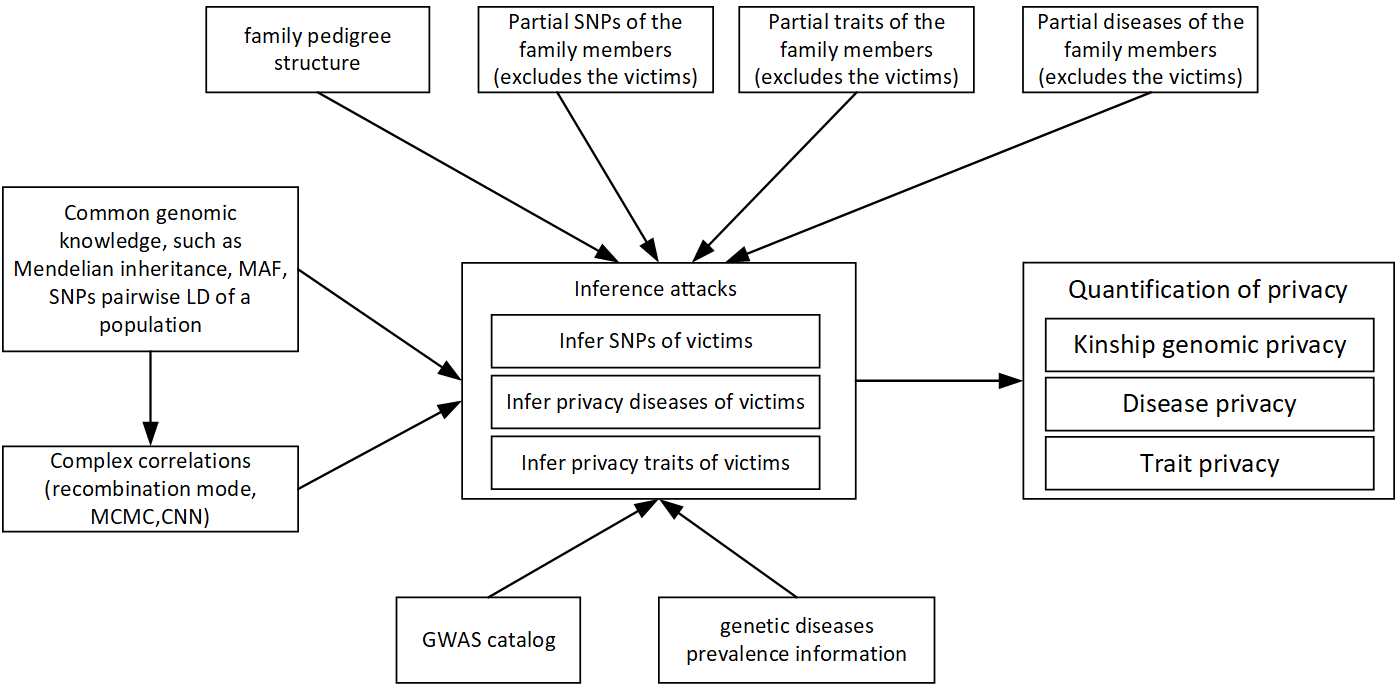
\includegraphics[width=0.95\linewidth]{./figures/attack-framework.png}
	\centering
	\caption{亲属基因组属性隐私分析推断框架}\label{fig:attack-framework}
\end{figure}

如图~\ref{fig:attack-framework}所示,敌手拥有一些背景知识信息,且观测到有关该家庭的一些基因组信息,然后他意图推断被攻击者的基因组相关属性隐私。 我们将攻击分为三个阶段:a)建立可以通过背景知识增强攻击的高阶相关性计算模型; b)推断有关被攻击者的私人信息,包括敌手尚未收集到的隐私SNP,私人特征和疾病; c)量化推断获取的隐私信息量。

\subsection{基因属性隐私分析模型}
提出的基因属性隐私分析推断攻击目的在于推断目标SNP值,特征和疾病信息。
给定观测值(~$\mathbf{X}_K$~,~$\mathbf{T}_K$~和~$\mathbf{D}_K$~和家族结构)和背景知识(孟德尔遗传定律函数~$\mathcal{F}_T(x_i^F,x_i^M,x_i^C)$~),次要等位基因概率~$\mathbf{P}$~,性状与SNP之间的关系~$\mathbb{T}$~,疾病与SNP之间的关系~$\mathbb{D}$~,遗传疾病的患病率~$\mathbb{P}$~,重组模型~$\mathbf{F}$~的公式以及种群的SNP),该推断攻击可公式化为计算未知变量~$\mathbf{X}_U$~,~$\mathbf{T}_U$~和~$\mathbf{D}_U$~的边缘概率分布。
因此,利用联合概率分布函数可以获得未知变量的边缘概率分布。

\begin{equation}\label{eq:joint-pro}
\begin{aligned}
p(\mathbf{X}_U, \mathbf{T}_U, \mathbf{D}_U | \mathbf{X}_K, \mathbf{T}_K, \mathbf{D}_K, T, \mathcal{F}_T(x_i^F,x_i^M,x_i^C), \mathbf{P}, \mathbb{T}, \mathbb{D}, \mathbb{P}, \mathbf{F})
\end{aligned}
\end{equation}

假设~$\hat{\mathbf{X}_U}$~是~$\mathbf{X}_U$~的推断值,则可以将公式~\ref{eq:joint-pro}解析为两步:1)公式~\ref{eq:joint-pro};2)公式~\ref{eq:joint-pro-Tu}和公式~\ref{eq:joint-pro-Du},即

\begin{equation}\label{eq:joint-pro-Xu}
p(\mathbf{X}_U | \mathbf{X}_K, \mathbf{T}_K, \mathbf{D}_K, T, \mathcal{F}_T(x_i^F,x_i^M,x_i^C), \mathbf{P}, \mathbb{T}, \mathbb{D}, \mathbb{P}, \mathbf{F})
\end{equation}

\begin{equation}\label{eq:joint-pro-Tu}
p(\mathbf{T}_U |\hat{\mathbf{X}_U}, \mathbf{X}_K, \mathbf{T}_K, \mathbf{D}_K, T, \mathcal{F}_T(x_i^F,x_i^M,x_i^C), \mathbf{P}, \mathbb{T}, \mathbb{D}, \mathbb{P}, \mathbf{F})
\end{equation}

\begin{equation}\label{eq:joint-pro-Du}
p(\mathbf{D}_U |\hat{\mathbf{X}_U}, \mathbf{X}_K, \mathbf{T}_K, \mathbf{D}_K, T, \mathcal{F}_T(x_i^F,x_i^M,x_i^C), \mathbf{P}, \mathbb{T}, \mathbb{D}, \mathbb{P}, \mathbf{F})
\end{equation}


然后,若将家庭成员~$i$~的SNP ~$j$~的边缘分布表示为~$p(x_{ij})$~,则~$\mathbf{X}_u$~的每个变量的边缘概率分布可以得到为

\begin{equation}\label{eq:joint-pro-Xu2}
\begin{aligned}
p(x_{ij})= \sum_{\mathbf{X}_U/\{x_{ij}\}} p(\mathbf{X}_U | \mathbf{X}_K, \mathbf{T}_K, \mathbf{D}_K, T,  \mathcal{F}_T(x_i^F,x_i^M,x_i^C), \mathbf{P}, \mathbb{T}, \mathbb{D}, \mathbb{P}, \mathbf{F})
\end{aligned}
\end{equation}


一般情况下,由于复杂度随项数的增加而呈指数增长,无法计算公式~\ref{eq:joint-pro-Xu2}。实际上,一个人拥有数百万个SNP,并具有许多性状和基因组疾病,从而使计算不可行。


基于因子图的方法是一种计算概率值~\cite{kschischang2001factor}的有效方法。此外,由于SNP之间的基因重组和相关关系在染色体中是局部性的,因此可将SNP、性状和疾病分为不同的分区进行计算。 因此,我们将联合概率分布分解为一组局部函数,每个函数通过将其作为变量来表示SNP序列、家庭成员、性状和疾病之间的依赖关系。 然后,通过在因子图上启动置信度传播,可以线性时间复杂度计算得到边缘概率分布。


在这里,我们为概率推断计算建立一个因子图。该图具有两种类型的节点(变量节点和因子节点)和连接节点的边。与文献~\cite{humbert2013addressing,humbert2017quantifying,deznabi2018inference}相似,在此因子图中设置了每个SNP ~$x_{i,j}$~的变量节点(~$x_{i,j}\in \mathbf{X}$~,~$i$~表示家庭成员ID,~$j$~表示家庭成员~$i$~的SNP ID)。但是本章模型使用四种类型的因子节点~\cite{deznabi2018inference}:(i)\emph{家族因子节点},代表家族关系(关于孩子和父母)和遗传,(ii)\emph{重组模型相关因子节点},代表SNP之间的重组模型相关性,正如第\ref{sec:backgrounds}节所述,它比其他类型的高阶相关性包含更多的信息,(iii)\emph{特征因子节点}代表SNP与个体特征之间的关系,以及(iv)\emph{疾病因子节点},代表SNP与个体基因组疾病之间的关系。本章中,\emph{相关性因子节点}与文献~\cite{humbert2013addressing}和文献~\cite{deznabi2018inference}的工作不同,我们利用重组模型来表示SNP的高阶相关性。如Marchini等~\cite{marchini2007newa}和Samani等~\cite{samani2015quantifying}所述,重组模型在验证和校正基因型标记~\cite{marchini2007newa}处的数据方面具有良好的性能,且因其包含重组和突变因子~\cite{samani2015quantifying},在预测隐藏的SNV方面具有更好的性能。本章我们将其直接用于构建因子图,并推断出与亲属关系相关的基因组隐私。此外,由于我们采用了GWAS目录和遗传疾病的患病率,所以用\emph{特征因子节点}和\emph{疾病因子节点}代替了~\cite{deznabi2018inference}中的\emph{表型因子节点} 来构建因子图。除了观测家族成员的特征和疾病,GWAS目录还可以分别提供SNP与特征和疾病之间的更多相关性,且遗传疾病的患病率可以提供一些其他信息来推断SNP的值。 GWAS中的常识是,疾病和性状与SNP序列~\cite{manolio2008a}有关,某些复杂的疾病由多个SNP序列和其他因素~\cite{climer2014a}决定。我们提出的因子图如图~\ref{fig:factor-graph}所示,变量和因子节点之间的联系描述如下。

\begin{itemize}
	\item 每个变量节点~$X_{i,j}$~具有其家族因子节点~$f_{i,j}$~,且二者相互连接。 若~$k$~是家庭中~$i$~的父母,则~$x_{k,j}$~(~$k \neq i$~)也连接到~$x_{i,j}$~。 若所观测到的家庭中~$i$~的父亲或母亲都没有,则因子节点~$f_{i,j}$~的度为1; 若只有~$i$~的父亲或母亲,则因子节点~$f_{i,j}$~的度为2; 若被观测家庭中有双亲~$i$~,则该度为3。 如图3中的示例所示,孩子的家庭因子节点的度数为3,因为他的父母都在这里,而父母的家庭因子节点的度数均为1,因为父亲或母亲的父母都未出现在被观测家庭中。
	\item 集合~$\mathbf{C}$~中的变量节点连接到重组模型相关因子节点~$rf_{i,\mathbf{C}}$~。 由于我们使用重组模型来训练SNP之间的相关性,因此所有SNP都可以视为与重组能力相关。设~$\mathbf{C}$~等于~$\mathbf{x}$~,其中包括一个人的所有SNP。 另一方面,Markov假设可以提高效率。 我们在实际计算步骤中使用基于Markov的计算方法。
	\item 若~$\mathbf{T}_{i,\alpha}$~中的SNP与特征~$T_{\alpha}$~( ~$T_{\alpha} \in \mathbf{t}$~)相关联,则集合~$\mathbf{T}_{i,\alpha}$~中的家族成员~$i$~的可变节点连接到特征因子节点~$tf_{i,\alpha}$~。 ~$\mathbf{T}_{i,\alpha}$~和 ~$\mathbf{T}_{j,\alpha}$~ (~$i \neq j$~)的SNP具有相同的基因座集合。 这意味着对于不同个体的特定特征,相关SNP的位点是相同的。 ~$\mathbf{T}_{i,\alpha}$~中的SNP数量可能大于1。换句话说,一个给定的性状与一个以上的SNP相关;另外,一个SNP也可能与一个以上的性状相关。 有时已经观测到家族成员的某些特征,有时没有。
	\item 若~$\mathbf{D}_{i,\beta}$~中的SNP与遗传疾病~$D_{\beta}$~(~$D_{\beta} \in \mathbf{d}$~)相关,则~$\mathbf{D}_{i,\beta}$~组中家族成员~$i$~的变量节点连接到性状因子节点~$df_{i,\beta}$~。 类似地,可能有不止一种SNP与给定的遗传疾病相关; 一个SNP也可能与一种以上疾病有关。有时已经从家族成员身上观测到了某些疾病,有时则没有。值得注意的是,对于特定疾病,即使相关SNP的位点对于不同的个体而言都是相同的,该疾病的当前结果也有所不同,因为该疾病也可能受到其他因素的影响。
	
\end{itemize}


若条件依赖性已经利用观测到的信息和公共信息给出,则因子图中变量节点全局分布~$p(\mathbf{X}_U | \mathbf{X}_K, \mathbf{T}_K,\mathbf{D}_K,~$~ ~$T, \mathcal{F}_T(x_i^F, x_i^M, x_i^C), \mathbf{P}, \mathbb{T}, \mathbb{D}, \mathbb{P}, \mathbf{F})$~可以分解为几个局部函数的乘积。 每个局部函数都有一个来自~$\mathbf{X}$~的变量节点子集作为参数。
\begin{equation}\label{eq:joint-pro-multi}
\begin{aligned}
p&(\mathbf{X}_U | \mathbf{X}_K, \mathbf{T}_K, \mathbf{D}_K, T, \mathcal{F}_T(x_i^F,x_i^M,x_i^C), \mathbf{P}, \mathbb{T}, \mathbb{D}, \mathbb{P}, \mathbf{F}) =   \\
& \frac{1}{Z}[\prod_{i \in \mathbf{S}} \prod_{j \in \mathbf{SID}} f_{i,j}(x_{i,j}, \Theta(x_{i,j}),\mathcal{F}_{R}(x_{M,j},x_{F,j}, x_{C,j},\mathbf{P})] \times [\prod_{i \in \mathbf{S}}rf_{i,\mathbf{C}}(x_{i,1},x_{i,2},...,x_{i,m},\mathbf{F})]  \\
&  \times [\prod_{i \in \mathbf{S}}\prod_{\alpha \in \mathbf{t}}tf_{i,\alpha}(\Psi(i,\alpha),\mathbb{T})] \times [\prod_{i \in \mathbf{S}}\prod_{\beta \in \mathbf{d}}df_{i,\beta}(\phi(i,\beta),\mathbb{D},\mathbb{P}))]
\end{aligned}
\end{equation}
其中,~$Z$~是标准化常数,~$\Theta(x_{i,j})$~是~$\mathbf{T}$~中~$i$~的父代的SNP ~$j$~值的变量集,~$\Psi(i,\alpha)$~是个体~$i$~与特征~$\alpha$~相关的SNP值的变量集,~$\phi(i,\beta)$~是变量集 ~$i$~个体的SNP值与疾病B相关。

公式~\ref{eq:joint-pro-multi}的因式分解基于置信传播规则,变量和因子节点之间传递的信息可用于构造迭代置信传播算法,以计算全局边缘概率分布。 令~$\mathbf{X}^v=\{x_{i,j}^v: i\in \mathbf{S}, j \in \mathbf{SID}\}$~是表示算法在~$V^{th}$~迭代时变量节点值的变量集合, 我们将消息描述如下,

\begin{itemize}
	\item 消息~$\mu_{i\rightarrow k}^{v}(x_{i,j}^{v})$~(从变量节点~$i$~到因子节点~$k$~)表示了在~$V^{th}$~迭代中 ~$X_{i,j}^v=l$~ (~$l \in {0,1,2}$~)的概率,。
	\item 从家族因子节点到变量节点的消息表示为~$\lambda_{k \rightarrow i}^v(x_{i,j}^v)$~,其表示在~$V^{th}$~迭代中,给定~$\mathcal{F}_{R}(x_{M,j},x_{F,j}, x_{C,j})$~,~$\mathbf{P}$~以及与单个~$i$~的相应家庭因子节点关联的家庭成员的SNP的~$j$~值时,~$X_{i,j}^v=l$~ (~$l \in {0,1,2}$~)的概率。
	\item 从重组模型相关因子节点到变量节点的消息表示为~$\beta_{k \rightarrow i}^v(x_{i,j}^v)$~,其表示在~$V^{th}$~迭代中,给定基于SNP之间基于建模重组率的相关性时,~$X_{i,j}^v=l$~ (~$l \in {0,1,2}$~)的概率。
	\item 从特征因子节点到变量节点的消息表示为~$\varphi_{k \rightarrow i}^v(x_{i,j}^v)$~,表示在~$v^{th}$~迭代中 ,给出单个~$i$~的特征~$t_k$~以及相应特征与SNP ~$j$~的关联~$\mathbb{T}$~时, ~$x_{i,j}^v=l$~ (~$l \in {0,1,2}$~)的概率。
	\item 从疾病因子节点到变量节点的消息表示为~$\tau_{k \rightarrow i}^v(x_{i,j}^v)$~,其表示在~$v^{th}$~迭代中,给定个体~$l$~的疾病~$d_k$~、相应疾病的~$\mathbb{D}$~与SNP~$j$~的关联、以及疾病的患病概率分布~$\mathbb{P}$~的情况下, ~$x_{i,j}^v=l$~ (~$l \in {0,1,2}$~)的概率。
	
\end{itemize}

\subsection{家族基因属性隐私分析示例}

\begin{figure}[htbp]
	\centering
	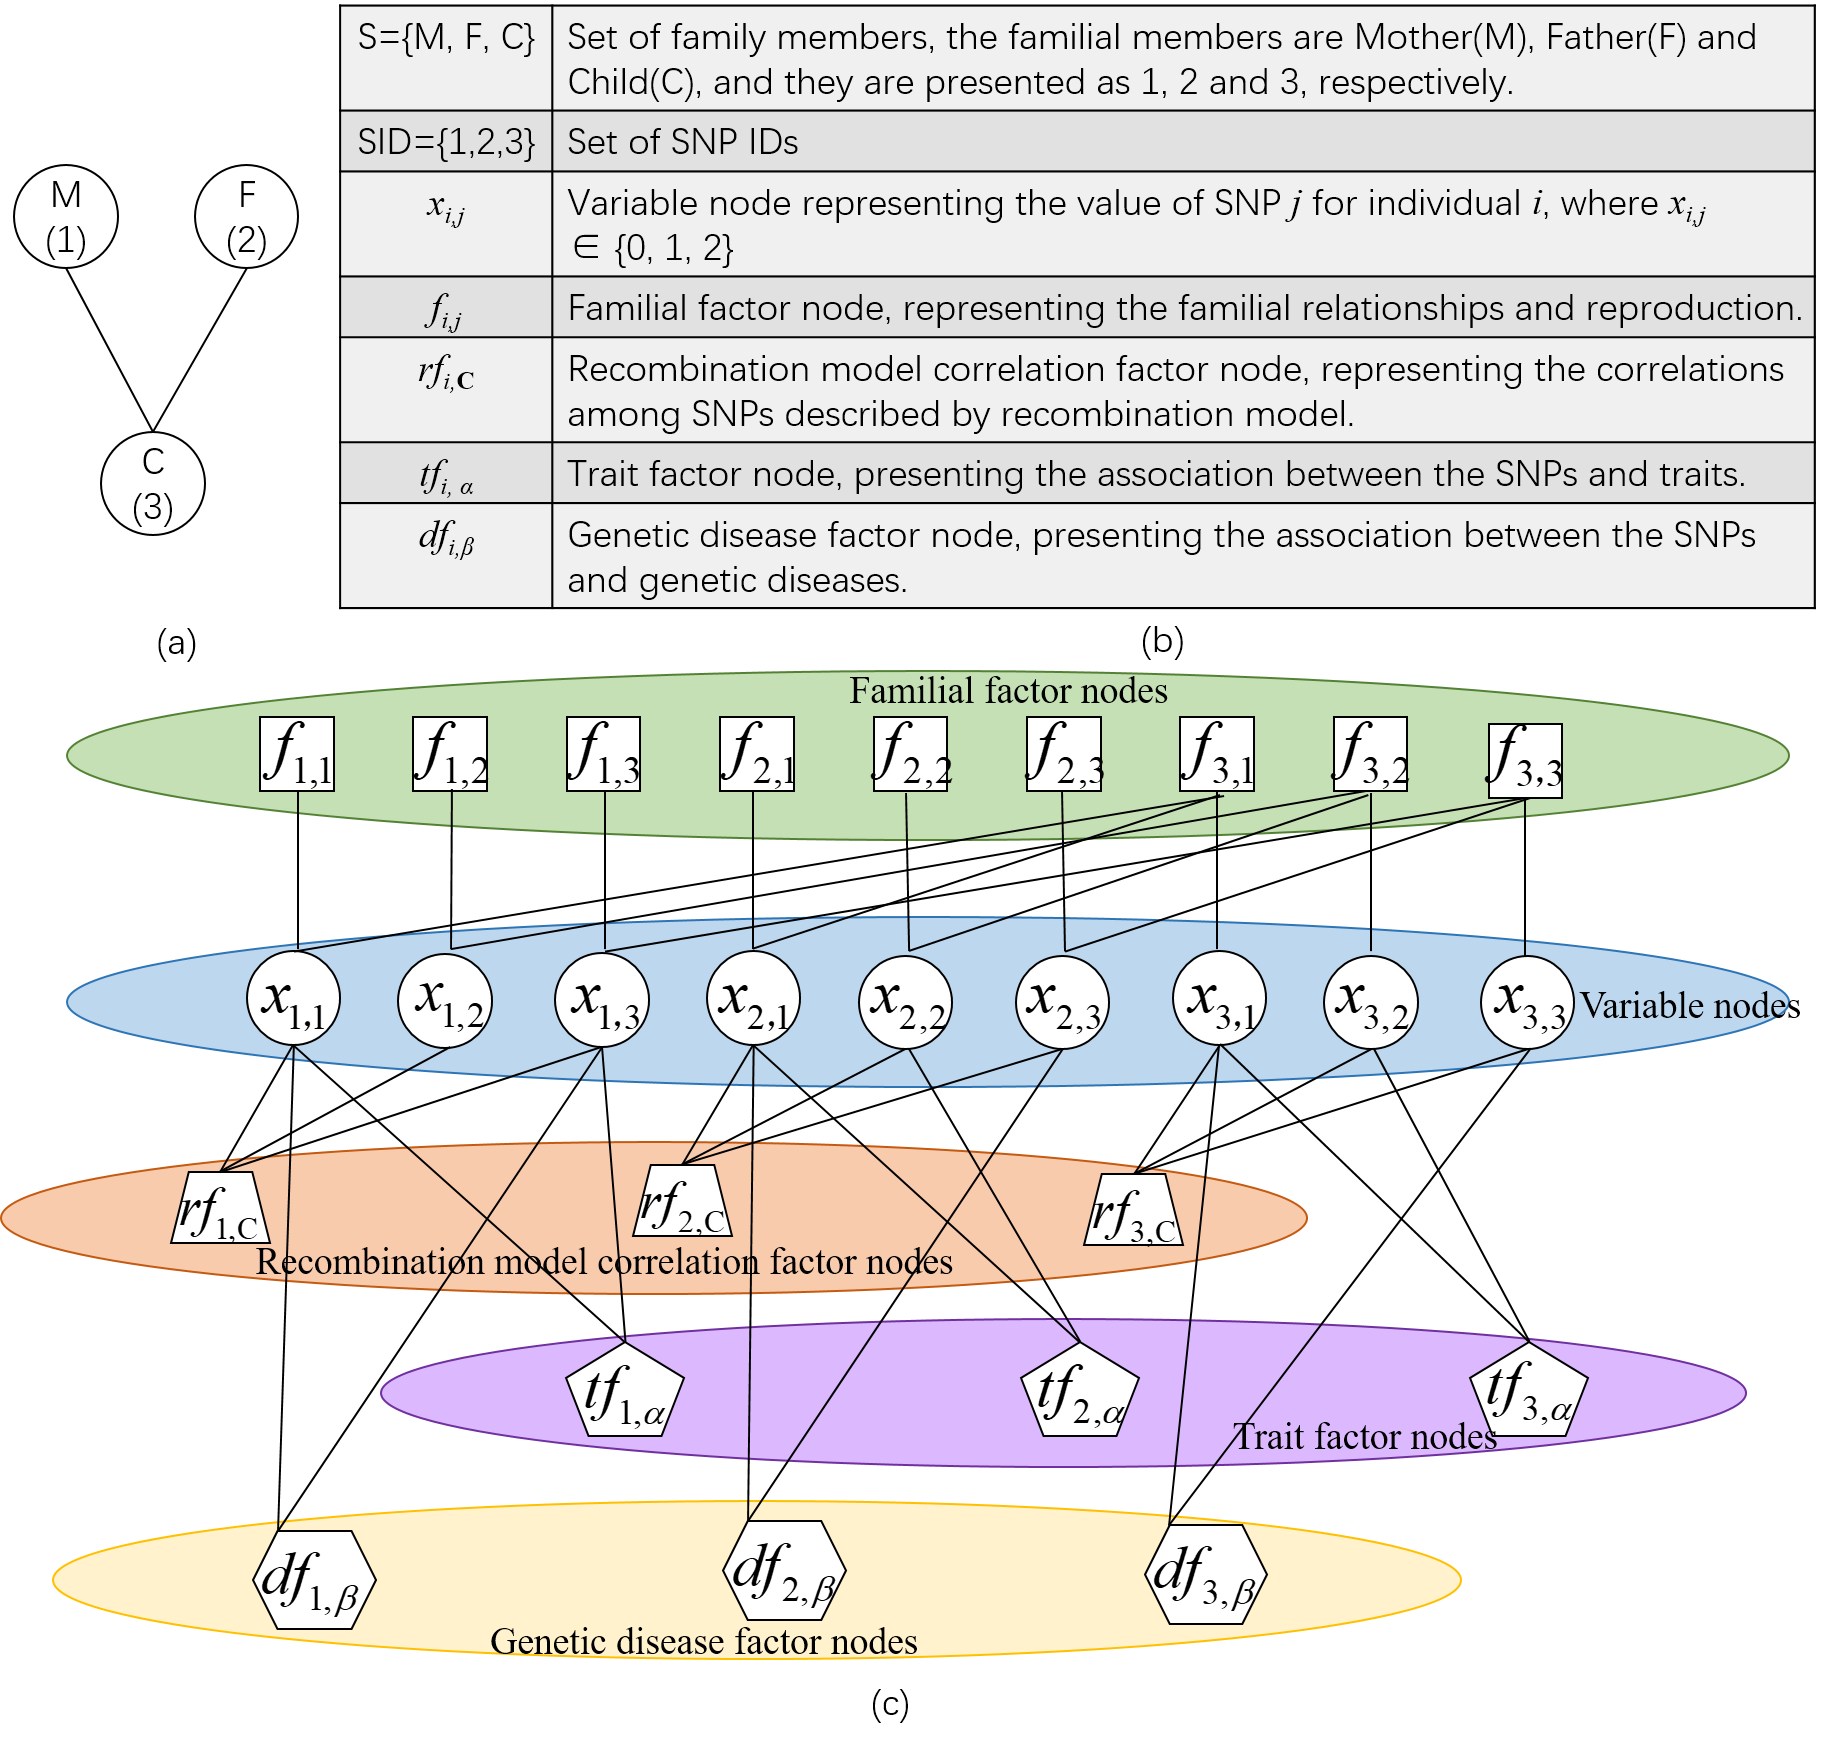
\includegraphics[width=0.95\linewidth]{./figures/factor-graph.png}
	\centering
	\caption{三个成员家族3个SNP的因子图示例}\label{fig:factor-graph}
\end{figure}

为了更好地理解该公式,我们仅以母亲,父亲和孩子以及3个SNP为例选择一棵家谱。构建的三人家族谱系、SNP序列和因子图如图3所示,其中子图 (a) 是三个成员家族的结构图;(b)是因子图中的符号;(c) 是因子图和节点之间传递的消息。在因子图中,~$i=1$~,~$i=2$~和~$i=3$~分别表示母亲,父亲和孩子,这3个SNP分别表示为~$j=1$~,~$j=2$~和~$j=3$~。在这里,我们描述了表示母亲的第一个SNP的变量节点(~$X_{1,1}$~),孩子的家庭因子节点(~$f_{3,1}$~)和重组模型之间的消息交换母亲的相关因子节点(~$rf_{1,\mathbf{C}}$~),母亲的特征因子节点(~$tf_{1,\alpha}$~)和母亲的疾病因子节点(~$df_{1,\beta}$~)。我们假设所有SNP都包含在集合~$\mathbf{C}$~中,特征~$\alpha$~与SNP 1和2相关,而疾病~$\beta$~与SNP 2和3相关。在图~\ref{fig:factor-graph}(c)中,通过置信传播算法迭代变量节点和因子节点之间的消息,并在每次迭代中更新对~$\mathbf{X}_u$~中目标SNP值的置信概率,直到收敛为止。我们分别用~$i$~,~$k$~,~$z$~,~$s$~和~$T$~表示变量和因子节点~$X_{1,1}$~,~$f_{3,1}$~,~$rf_{1,\mathbf{C}}$~,~$tf_{1,\alpha}$~和~$df_{1,\beta}$~。


\emph{来自变量节点的消息。}算法由变量节点开始执行,生成并发送消息到邻居节点。变量节点~$i$~通过乘以从邻居那里收到的除家族因子节点~$k$~之外的所有信息,生成消息~$\mu_{i \rightarrow k}^v(x_{1,1}^v)$~。 可以类似地生成到其他邻居的变量节点~$i$~,然后在~$V^{th}$~迭代中从变量节点~$i$~到家庭因子节点~$k$~的消息是

\begin{equation}\label{eq:variable-message}
\mu_{i \rightarrow k}^v(x_{1,1}^v)= \frac{1}{Z} \times
%\prod_{w \in \{f_{1,1}\}} \lambda_{w \rightarrow i}^{v-1}(x_{1,1}^{v-1}) \times
\beta_{z \rightarrow i}^{v-1}(x_{1,1}^{v-1}) \times
\varphi_{s \rightarrow i}^{v-1}(x_{1,1}^{v-1})
\end{equation}
其中,~$Z$~是归一化常数,对每个变量节点的每个邻居重复此计算。若已知~$X_{1,1}$~的值,则消息~$\mu_{i \rightarrow k}^v(x_{1,1}^v =l)$~(~$l\in \{0,1,2\}$~)将为常数1。在这里,我们不使用消息~$\lambda_{k \rightarrow i}^{v-1}(x_{1,1}^{v-1})$~和 ~$\varphi_{t \rightarrow i}^{v-1}(x_{i,j}^{v-1})$~生成~$\mu_{i \rightarrow k}^v(x_{1,1}^v)$~,因为其在示例中没有实际意义。值得注意的是,若图中包含母亲的父母,则应使用消息~$\lambda$~生成~$\mu_{i \rightarrow k}^v(x_{1,1}^v)$~; 若有任何疾病与~$X_{1,1}$~相关,则还应使用来自那些疾病因子节点的消息~$\varphi$~。

\emph{来自家庭因子节点的消息。}从家庭因子节点~$k$~到~$V^{th}$~处变量节点~$i$~的消息,使用置信传播的原理形成迭代

\begin{equation}
\label{eq:familial-message}
\lambda_{k \rightarrow i}^v(x_{1,1}^v) =  \sum_{\{x_{2,1},x_{3,1}\}}f_{3,1}(x_{1,1},\Theta(x_{1,1}),\mathcal{F}_{R}(x_{M,j},x_{F,j}, x_{C,j},\mathbf{P}) 
\times \prod_{y\in \{x_{2,1},x_{3,1}\}} \mu_{y \rightarrow k}^v(x_{1,1}^v)
\end{equation}

在公式~\ref{eq:familial-message}中,~$f_{3,1}(x_{1,1},\Theta(x_{1,1}),\mathcal{F}_{R}(x_{M,j},x_{F,j}, x_{C,j},\mathbf{P})$~与~$p(x_{1,1}| x_{2,1},x_{3,1},\mathcal{F}_{R}(x_{M,j},x_{F,j}, x_{C,j},\mathbf{P})~$\\成正比,且可以通过图~\ref{fig:Mendelian-law}所示的继承定律进行计算。若特定SNP的程度为1,则家族因子节点仅取决于其次要等位基因频率 相应的SNP。 对每个家庭因子节点的每个邻居重复此计算。


\emph{来自重组模型相关因子节点的消息。} 在~$V^{th}$~迭代中形成了从重组模型相关因子节点~$z$~到变量节点~$i$~的消息。

\begin{equation}\label{eq:relavtes-information}
\beta_{k \rightarrow i}^v(x_{1,1}^v) = \sum_{\{x_{1,2},x_{1,3}\}}rf_{1,\mathbf{C}}(x_{1,1},x_{1,2},x_{1,3},\mathbf{F},) \times  \prod_{y \in \{2,3\}} \mu_{x_{1,y} \rightarrow k}^v(x_{1,y}^v)
\end{equation}

为每个重组模型相关因子节点的每个邻居生成~$\beta$~条消息。 在本章中,我们使用基于重组率的模型来训练SNP之间的相关性。 我们通过使用适合二倍体基因型~\cite{marchini2007newa}的重组模型来实现相关性。

\emph{来自特征因子节点的消息。} 在~$V^{th}$~迭代中,从特征因子节点~$s$~到变量节点~$i$~的消息为

\begin{equation}
\label{eq:trait-message}
\varphi_{s \rightarrow i}^v(x_{1,1}^v) =  \sum_{\{x_{1,2}\}}tf_{1,\alpha}(x_{1,1},x_{1,2},\mathbb{T}) \times  \prod_{y \in \{2\}} \mu_{x_{1,y} \rightarrow s}^v(x_{1,y}^v)
\end{equation}

在此示例中,特征~$\alpha$~与母亲的SNP序列 ~$x_{1,1}$~和~$x_{1,2}$~相关联,
 函数~$\Psi(1,\alpha)$~用于获取与母亲的特征~$\alpha$~相关的SNP。函数~$tf_{1,\alpha}(x_{1,1},x_{1,2},\mathbb{T})$~是根据SNP序列 ~$X_{1,1}$~与~$X_{1,2}$~关联特征、以及遗传特征与SNP序列 ~$\mathbb{T}$~之间的关系来计算的。本章中,敌手可以利用GWAS目录来形成遗传特征与SNP之间的关系,并观测家族成员的生物学特征。

\emph{来自遗传疾病因子节点的消息。}在~$V^{th}$~迭代中,从遗传疾病因子节点~$T$~到变量节点~$i$~的消息为

\begin{equation}
\label{eq:disease-messages}
\tau_{s \rightarrow i}^v(x_{1,1}^v) =  \sum_{\{x_{1,3}\}}df_{1,\beta}(x_{1,1},x_{1,3},\mathbb{D},\mathbb{P}) \times  \prod_{y \in \{3\}} \mu_{x_{1,y} \rightarrow s}^v(x_{1,y}^v)
\end{equation}

在此示例中,疾病~$\beta$~与母亲~SNP序列 ~$X_{1,1}$和~$X_{1,3}$相关。 函数~$\phi(1,\beta)$~用于获取与母亲疾病~$\beta$~相关的SNP。 函数~$df_{1,\beta}(x_{1,1},x_{1,3},\mathbb{D}, \mathbb{P})$~是根据SNP ~$X_{1,1}$~和~$X_{1,3}$~与相应疾病的关联、疾病与SNP之间的关系~$\mathbb{D}$、以及遗传疾病的发病概率分布~$\mathbb{P}$~来计算的。
值得注意的是,即使性状和遗传疾病都与SNP相关,遗传疾病也得到了进一步的学习,且可以从遗传领域获得更多信息。 在本章中,敌手可以收集GWAS目录和遗传疾病的患病率,且可以观测到有关家族成员的某些遗传疾病信息。

通过使用置信传播算法,因子图中的所有变量和因子节点都会生成其消息,并在每次迭代时发送给所有邻居。在每次迭代中计算每个变量节点的边缘概率,且当边缘概率收敛时算法应停止计算。
该算法的计算复杂度与因子图中变量或因子节点的数量呈线性关系。由于SNP之间的相关性始终是局部的(例如基于Markov链的依赖性),也就是说我们可以根据相关性将因子图划分为子图,然后可以通过并行处理进一步提高计算效率。此外,SNP之间的相关系数也可以同时进行预先计算。因此,通过同时处理相对较小的组(每个组的顺序远小于SNP的总数),可以进一步加快计算速度。


\section{关联基因序列数据属性隐私分析评价与对比} 


本节我们使用类似于文献~\cite{humbert2013addressing,deznabi2018inference}的方法对所提出的关联基因序列隐私推断模型进行评价。 首先,提出了度量基因组隐私的量化指标,然后描述了我们实验中使用的数据集,最后对实验结果进行了比较。

\subsection{隐私量化模型}

为了度量被攻击者的基因序列属性隐私, 可以使用诸如信息论之类的不同指标来评估隐私分析攻击的强度~\cite{marchini2007newa,shokri2011quantifying,serjantov2002towards}。我们从基因组水平、疾病水平和攻击者的不正确性,不确定性和不确定性递减方面评估所提出的基因序列隐私推断攻击模型。 其中,不正确性和不确定性也用在文献~\cite{humbert2013addressing}和文献~\cite{deznabi2018inference}中。

推断SNP的不正确性量化了敌手推断目标SNP序列集中个体SNP隐私值时的错误率。我们使用公式~\ref{eq:snp-entropy}表示平均错误率。

\begin{equation}
\begin{aligned}\label{eq:snp-error-rate}
E^i_j=\sum_{x^i_j=\in \{0,1,2\}}{p(x^i_j|\Psi)\|x^i_j - \hat{x}^i_j\|}
\end{aligned}
\end{equation}
其中~$X^i_j$~ 是推断的SNP的真实值,而 ~$\Psi$~ 是攻击者观测到的信息。不正确性度量标准量化敌手在其推断攻击中与SNP的实际值之间的距离。

可以通过推断SNP的熵来量化攻击者对基因序列属性隐私的不确定性。 在这里,我们使用正轨熵度量,该度量指标来自文献~\cite{humbert2013addressing}且类似于文献~\cite{deznabi2018inference}。

\begin{equation}
\begin{aligned}\label{eq:snp-entropy}
H^i_j=
\frac{-\sum_{x^i_j=\in \{0,1,2\}}{p(x^i_j|\Psi)log(p(x^i_j|\Psi))}}{log(3)}
\end{aligned}
\end{equation}

公式~\ref{eq:snp-entropy}可以描述敌手未观测到的SNP序列值得熵,且该度量量化了敌手对其推断攻击的信心。

不确定性下降量可以通过推断攻击获得的SNP序列值进行评估。在这里,我们使用本文第\ref{chap:entropy-metric-model}中的互信息公式,并用熵的差进行估计。

\begin{equation}\label{eq:snp-mutual-information}
\begin{aligned}
I^i_j=& -\sum_{x^i_j=\in \{0,1,2\}}p_{MAF}(x^i_j)log(p_{MAF}(x^i_j))  \nonumber \\
& - (-\sum_{x^i_j=\in \{0,1,2\}}{p(x^i_j|\Psi)log(x^i_j|\Psi)})
\end{aligned}
\end{equation}
其中 ~$p_{MAF}(x^i_j)$~ 是来自MAF的SNP的概率。 公式\ref{eq:snp-mutual-information}描述了推断攻击的熵递减量,该度量指标量化了敌手获得的SNP隐私信息量以及推断攻击模型的强度。

为了评估不正确性,必须事先知道SNP的真实值。即使这三个指标相互关联,也始终不可能获得被攻击者的真实基因组数据。 因此,我们还可以使用归一化的熵和互信息来量化个人的基因组隐私和攻击的力量。
我们为每个SNP计算从公式\ref{eq:snp-error-rate} 到公式\ref{eq:snp-mutual-information}的隐私度量指标,然后取未知集~$\mathbb{X}_{\mathbf{U}}$~计算结果的平均值。


\subsection{实验数据集}

在本章中,我们使用两种类型的数据和三个数据集。

类型I:基因组参照数据集

~$\bullet$~ 1000基因组计划


类型II:家族基因组数据


~$\bullet$~ CEPH/Utah Pedigree 1463 

~$\bullet$~ Manuel Corpas Family Pedigree 

\textbf{(1) 1000基因组计划数据集}

1000基因组计划(1000 Genomes Project )是一项国际研究,旨在建立人类遗传变异的最详细基因组数据目录。在数据集中,有来自不同族群的一千多名匿名个体的各种基因组信息。我们使用来自1000基因组计划的CEU人口数据,包括参与者22号染色体上的MAF和SNP序列数据。

\textbf{(2) CEPH/Utah Pedigree 1463数据集}

Humbert等~\cite{humbert2013addressing,humbert2017quantifying}和Deznabi等~\cite{deznabi2018inference}也使用了CEPH/Utah Pedigree 1463数据集~\cite{drmanac2010human}。
该家族的SNP数据均采用基因组变体(GVF)和变体召回 (VCF)格式。为了与已有的工作保持一致,我们也仅对该家族17个成员中的11个成员进行基因序列属性隐私分析。 整个家庭的家谱结构与数据集一起发布,且11个成员的关系如图~\ref{fig:CEPH-Utah-Pedigree}所示。在图~\ref{fig:CEPH-Utah-Pedigree}中,蓝色节点代表男性家族成员,其他节点代表女性家族成员。

\begin{figure}[htbp]
	\centering
	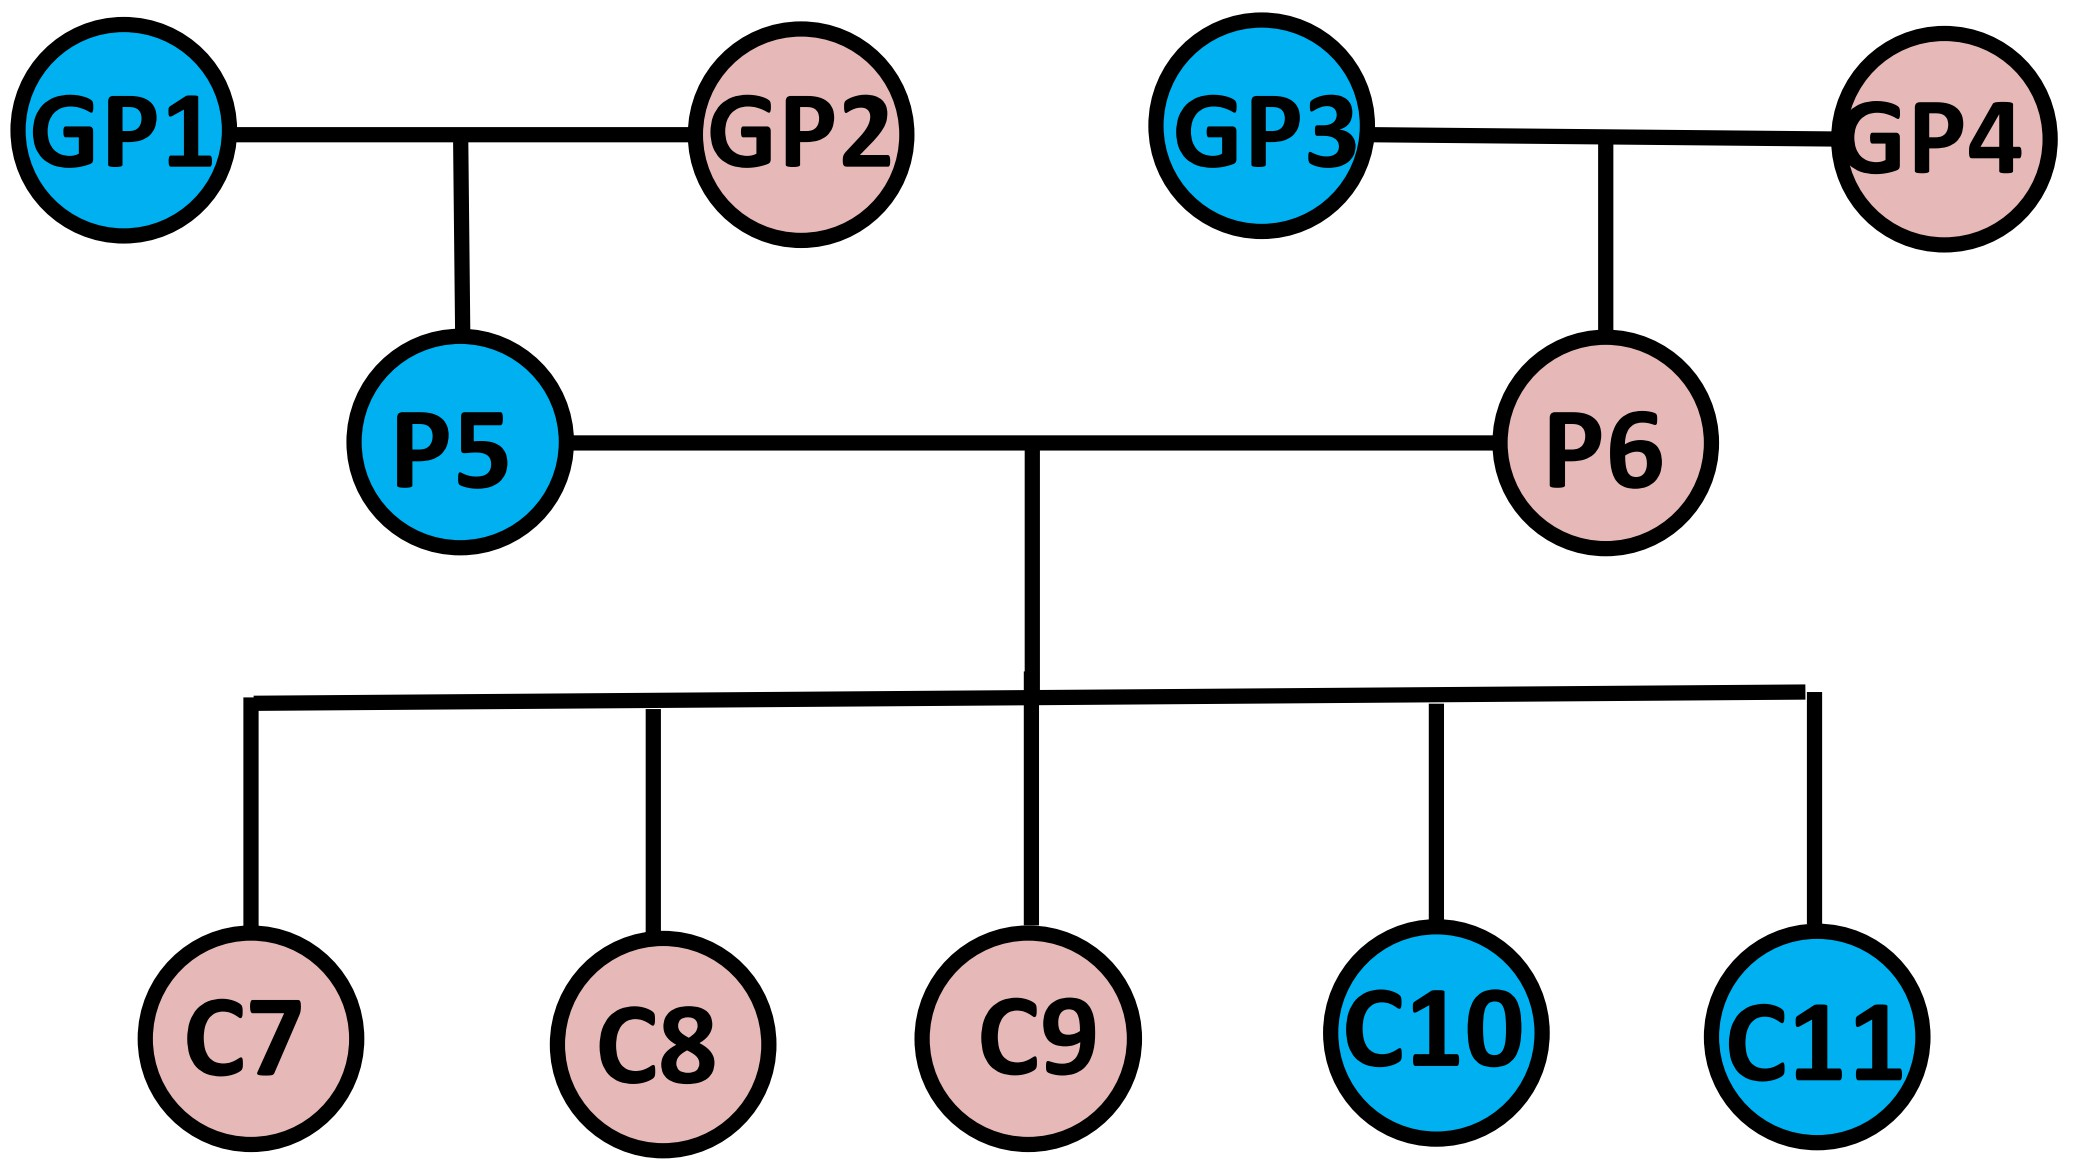
\includegraphics[width=0.6\linewidth]{./figures/CEPH-Utah-Pedigree.jpg}
	\centering
	\caption{CEPH/Utah Pedigree 1463家族谱系结构}\label{fig:CEPH-Utah-Pedigree}
\end{figure}

我们考虑了11个家庭成员的第22条染色体上物理位置15M到20M之间的1285个相邻SNP。在本章中,我们使用了比文献~\cite{deznabi2018inference}更高密度的基因组数据和更多SNP序列数据。 在文献~\cite{deznabi2018inference}中,仅筛选出了物理位置14.8M至17.5M之间的127个SNP,试验分析使用了100个SNP。

\textbf{(3) Manuel Corpas家族谱系数据集}

Manuel Corpas以变体召回格式 (VCF)公布了其家族的DNA数据。该数据集由家庭的5个成员(父亲、母亲、儿子、女儿和姨妈)组成,Deznabi等~\cite{deznabi2018inference}也使用了该数据集。该家族的谱系结构如图5所示,蓝色结点代表男性家族成员,其他结点代表女性家族成员。
我们将分析9个家族成员第22条染色体上物理位置15M到20M之间的679个相邻SNP。 对于祖父母缺失的SNP数据,我们利用父母和姨妈的SNP序列数据,基于孟德尔遗传定律和MAF对这两人的基因组数据进行了模拟生成。

\begin{figure}[htbp]
	\centering
	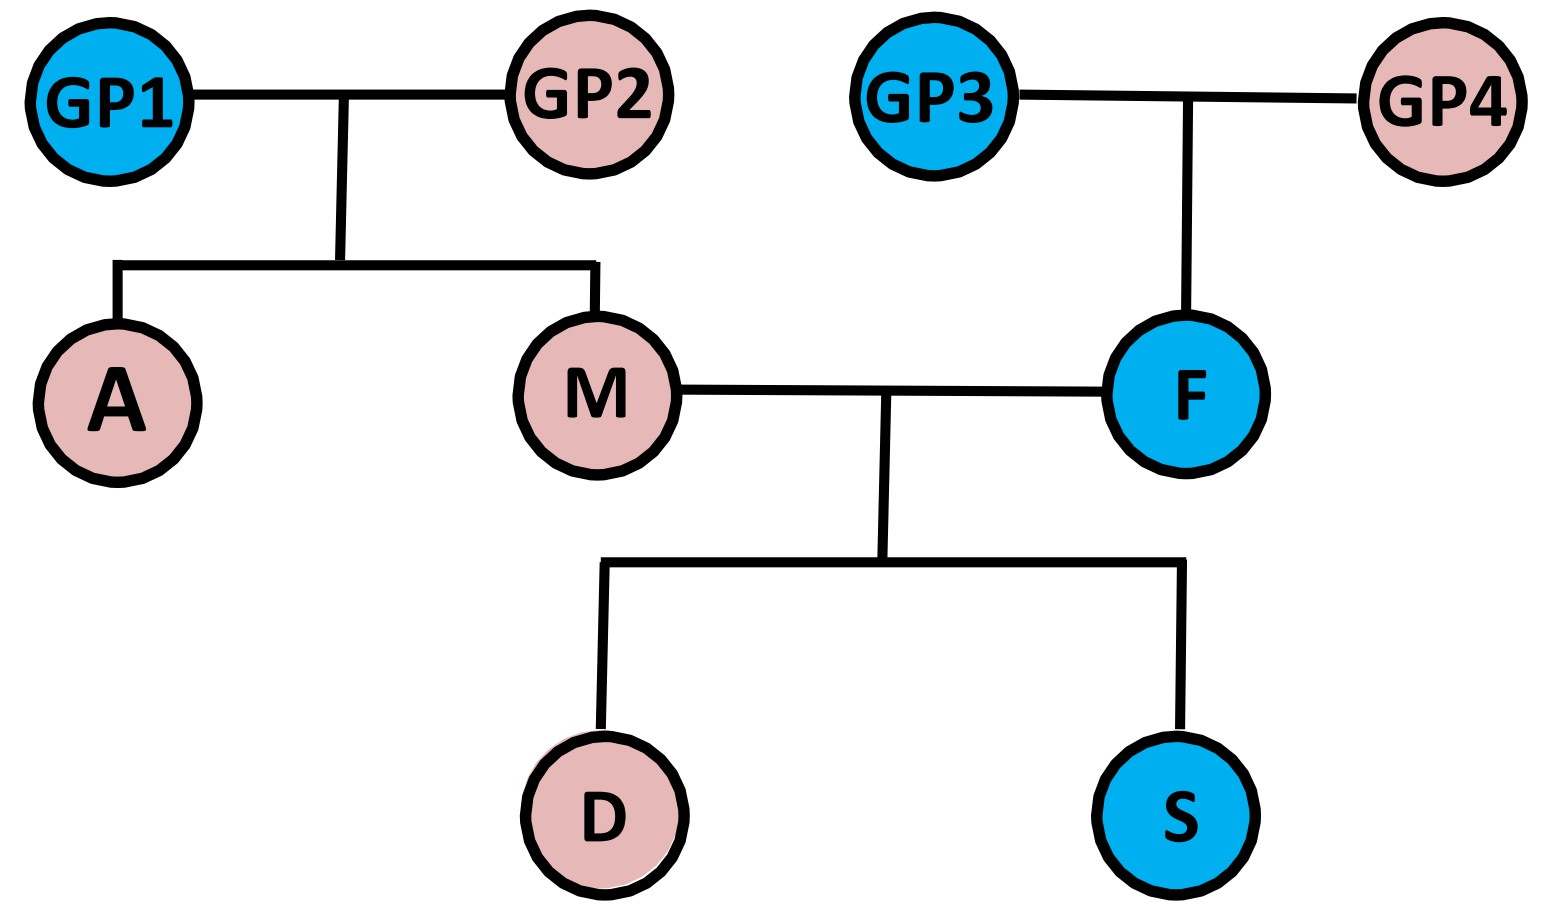
\includegraphics[width=0.6\linewidth]{./figures/Manuel-Corpas-Family-Pedigree.jpg}
	\centering
	\caption{Manuel Corpas家族谱系结构}\label{fig:Manuel-Corpas-Family-Pedigree}
\end{figure}

\subsection{实验结果分析}

本小节中,我们使用置信传播算法对所提出的基因序列数据隐私推断攻击算法进行分析,分别对两个家族的基因组数据集中的基因属性隐私进行分析。

\textbf{(1) CEPH/Utah Pedigree 1463实验结果}

在第一个实验中,我们假设被攻击者是P5,在1679个SNP中,我们随机隐藏了CEPH/UTAH家族其他成员的50\%SNP。我们假设攻击者知道所观测到的家庭成员的一些基因组相关性状和疾病,尝试通过增加攻击者的背景知识来推断P5的SNP序列属性值。 尽管大家都知道许多人类特征和疾病都与SNP序列取值相关,例如,口头陈述性记忆与Rs5747035相关、神经纤维瘤病与Rs121434260相关、克罗恩病与Rs4820425相关,但是有关CEPH / UTAH家庭成员的这些信息是未知的。 在该实验中,我们用概率随机模拟了家族成员的特征和疾病,并将这些信息用于基因序列属性隐私分析推断攻击。 真实的特征和疾病信息可以从Snpedia网站和欧洲分子生物学实验室下载。模拟信息对推断攻击的表示将与家庭成员的真实信息相吻合。 在该实验中,为了显著考察个体特征、疾病对SNP取值推断的影响,我们模拟了0.3\%的SNP和0.4\%的SNP与不同的性状和疾病相关关系。

\begin{figure}[htbp]
	\centering
	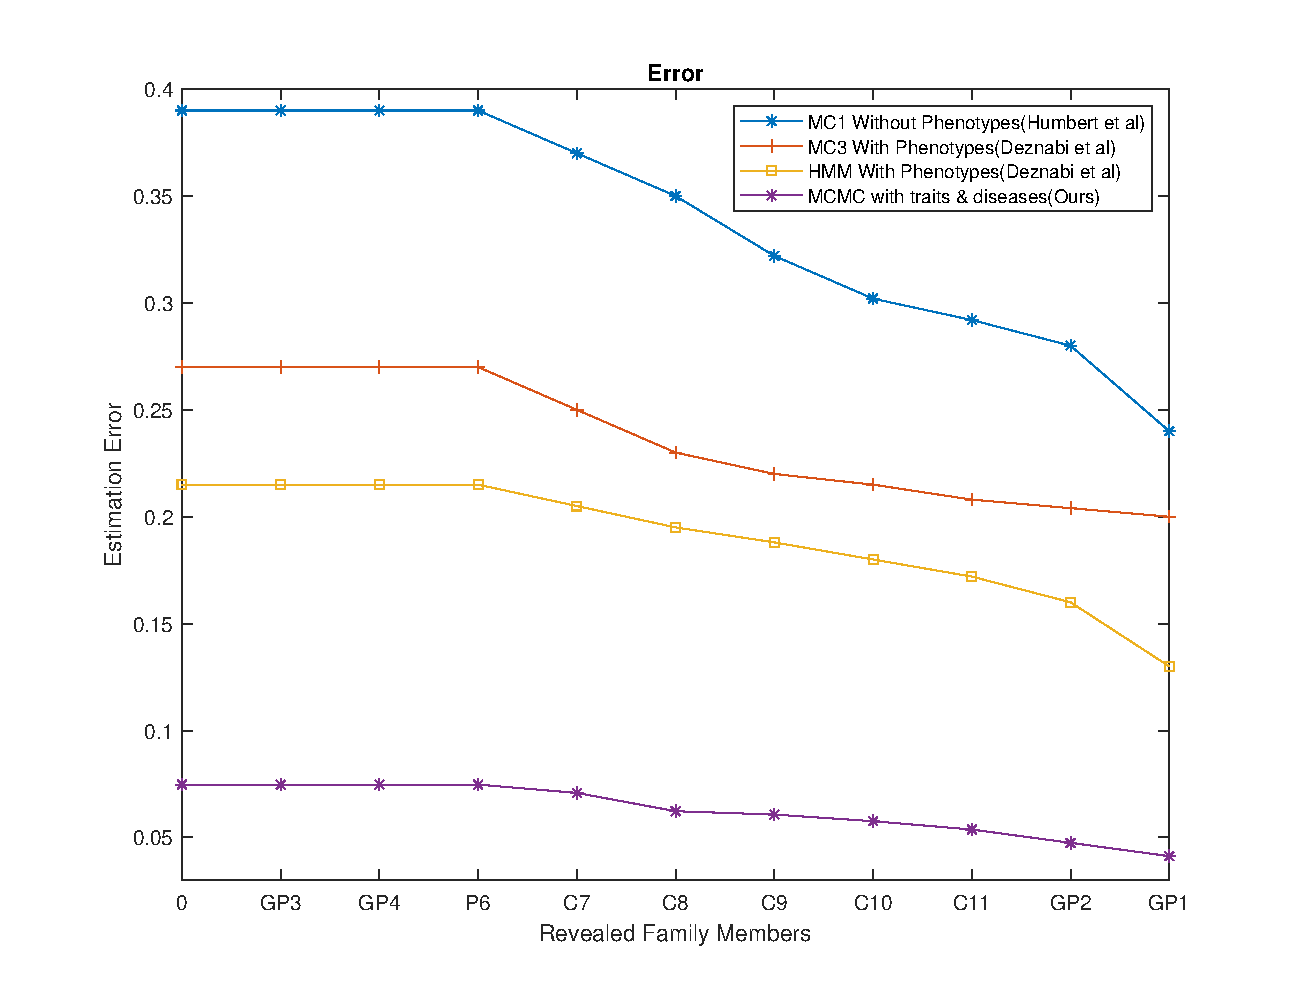
\includegraphics[width=0.8\linewidth]{./figures/P5error1.eps}
	\centering
	\caption{攻击者对P5的SNP序列属性隐私推断错误率下降情况对比}\label{fig:P5error1}
\end{figure}


我们首先披露观测到的家庭成员中50\%的SNP序列数据,并考察所提出的基因序列属性隐私分析推断攻击的强度。在文献~\cite{humbert2013addressing,humbert2017quantifying}和~\cite{deznabi2018inference}中观测到的家庭成员的SNP序列数据披露顺序是相同的,即从P5的亲属关系最远的一个成员到最亲近的一个成员进行SNP序列披露。 我们分别在图~\ref{fig:P5error1}和图~\ref{fig:P5entropy1}中显示了当50\%SNP序列值被随机隐藏时,先后披露不同家族成员SNP序列数据,攻击者对被攻击者的SNP序列取值的错误率和不确定性递减的结果。 图中,MC1(一阶Markov链或成对连锁不平衡) 代表了Humbert等的工作,其考虑了SNP间成对连锁不平衡关联;MC4(4阶Markov链)代表了Deznabi等的工作,其考虑了基因表型信息,应用了简单隐Markov模型。MCMC代表了本章的工作,应用了特征和疾病信息。本章工作在攻击者的不正确性和不确定性方面都大大提升了基因属性隐私分析推断攻击的强度。当50\%SNP序列值被随机隐藏时,先后披露不同家族成员SNP序列数据,攻击者获得的基因组隐私递增情况 如图~\ref{fig:P5privacyloss1}所示,它与图~\ref{fig:P5error1}和图~\ref{fig:P5entropy1}中所示的前两个度量指标一致。随着更多的亲属向敌手披露个人基因序列数据,被攻击者泄露给敌手的个人基因序列隐私也会越多。

\begin{figure}[htbp]
	\centering
	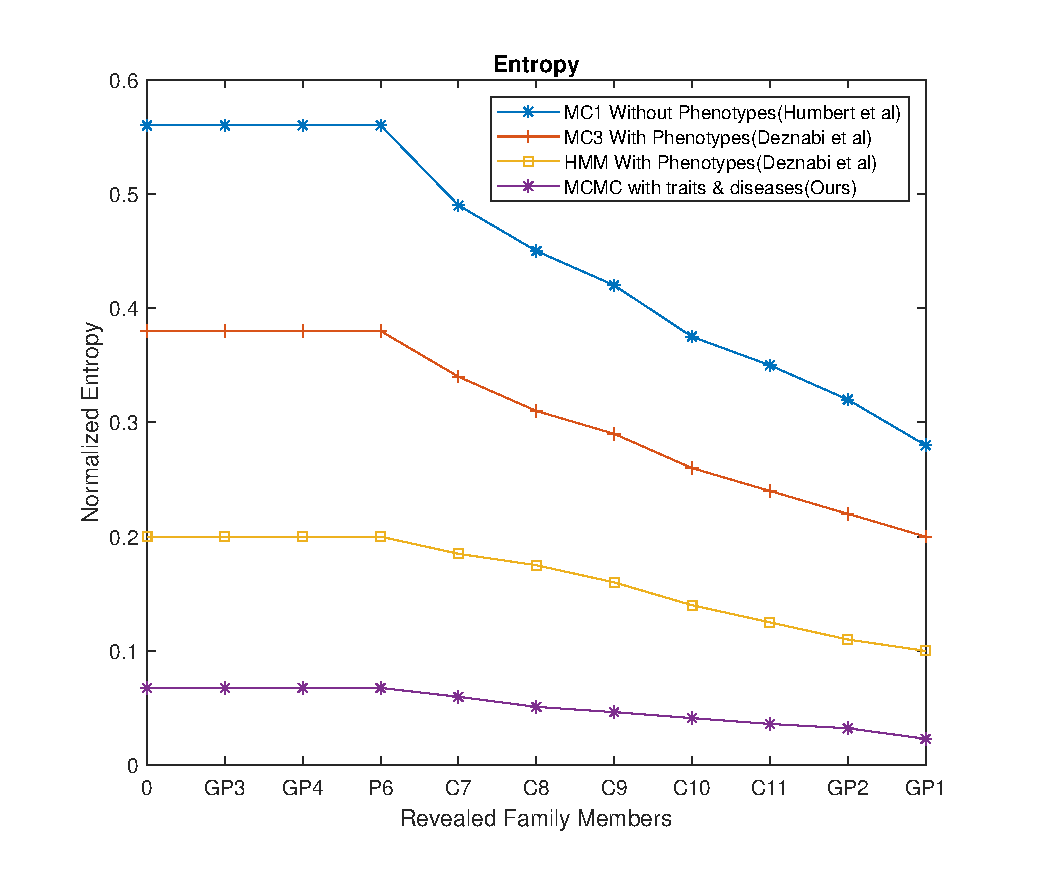
\includegraphics[width=0.8\linewidth]{./figures/P5entropy1.eps}
	\centering
	\caption{攻击者对P5的SNP序列属性隐私推断不确定性下降情况对比}\label{fig:P5entropy1}
\end{figure}

\begin{figure}[htbp]
	\centering
	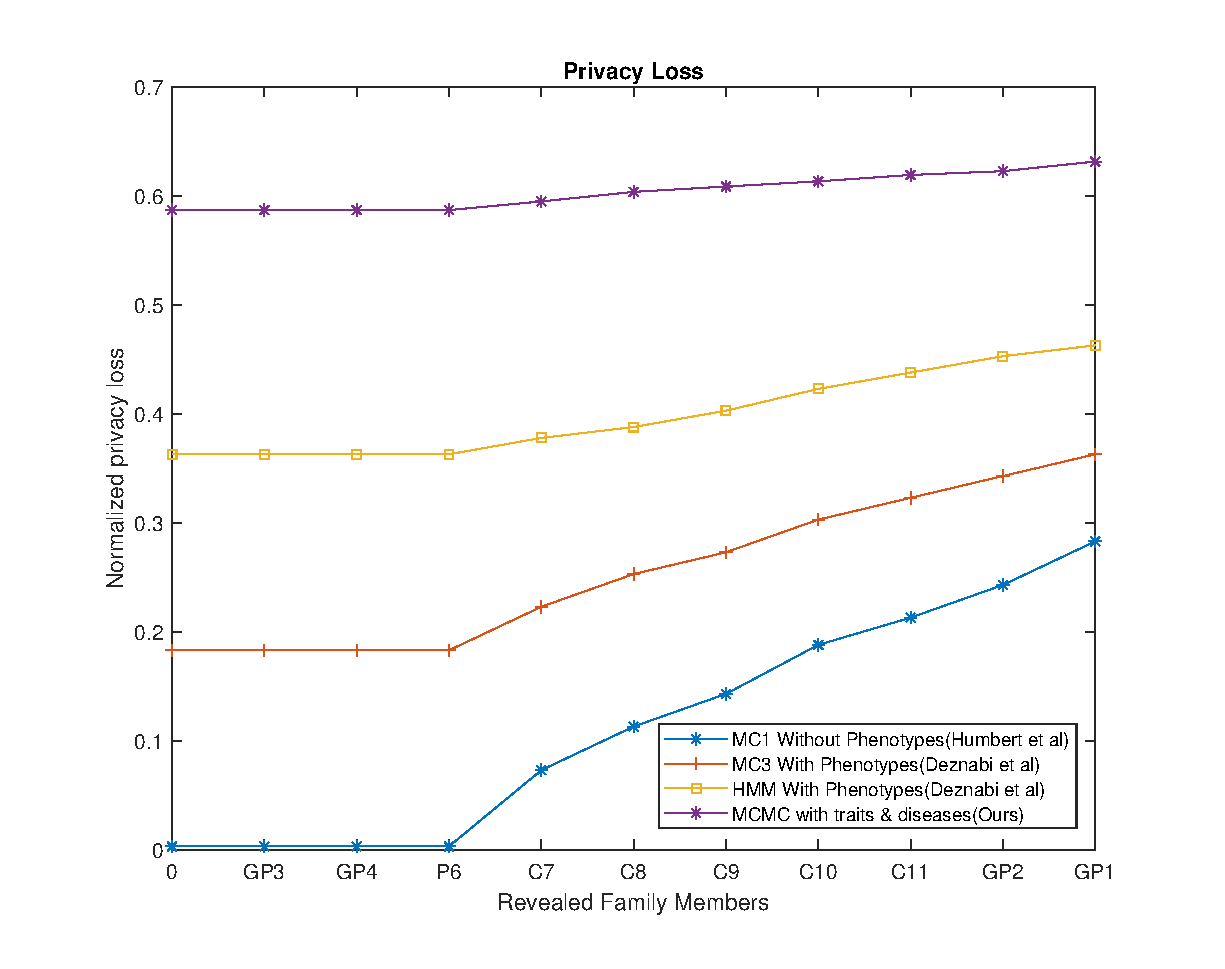
\includegraphics[width=0.8\linewidth]{./figures/P5privacyloss1.eps}
	\centering
	\caption{攻击者对P5的SNP序列属性隐私推断隐私信息量增加情况对比}\label{fig:P5privacyloss1}
\end{figure}


\begin{figure}[htbp]
	\centering
	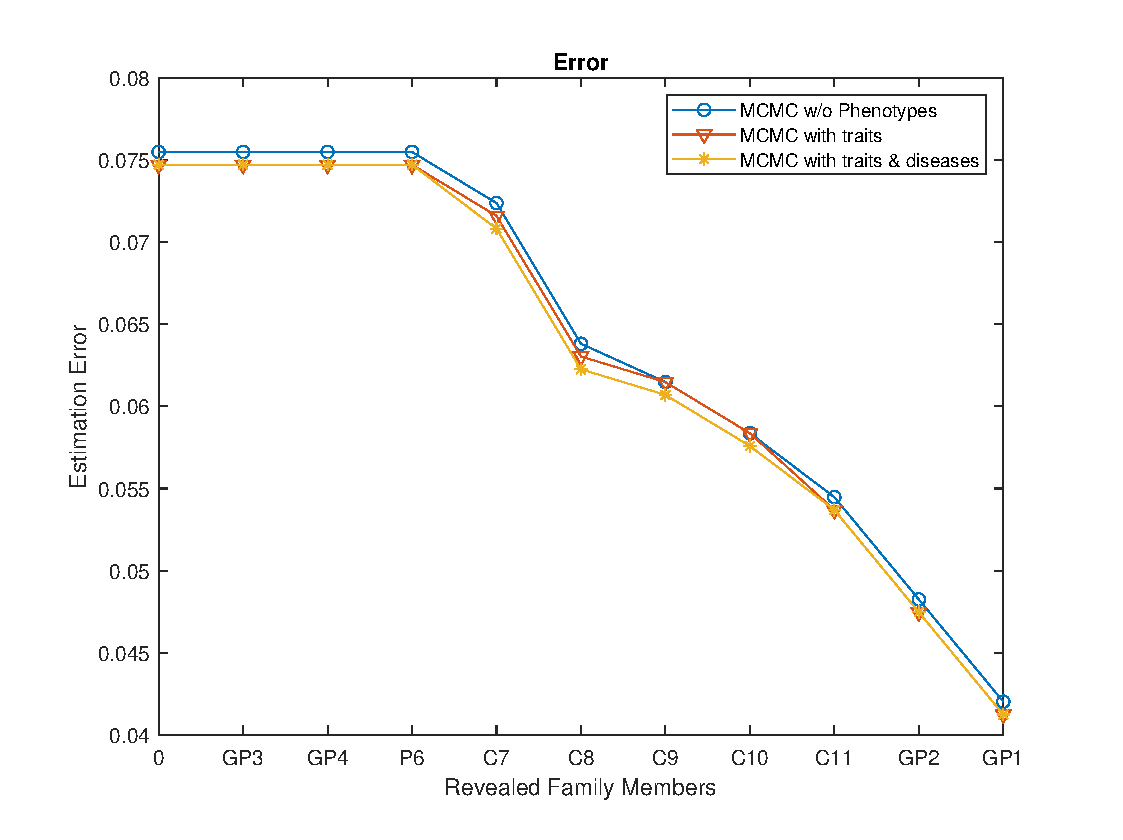
\includegraphics[width=0.8\linewidth]{./figures/P5error2.eps}
	\centering
	\caption{附加特征与疾病信息时,攻击者对P5的SNP序列属性隐私推断错误率降低情况对比}\label{fig:P5error2}
\end{figure}


其次,为了考察基因表征信息和疾病信息的对被攻击者基因序列属性隐私泄露的影响情况,我们针对提出的推断攻击模型进行了各种附加信息的实验。随机隐藏50\%SNP序列值,先后披露不同家族成员SNP序列数据、相关性状和疾病信息,攻击者对被攻击者的SNP序列取值推断结果的错误率和不确定性递减对比情况如图~\ref{fig:P5error2}和图~\ref{fig:P5entropy2}所示,可以看出攻击者获得的被观测家庭成员的信息越多,被攻击者向攻击者泄露的基因组隐私就越多。

\begin{figure}[htbp]
	\centering
	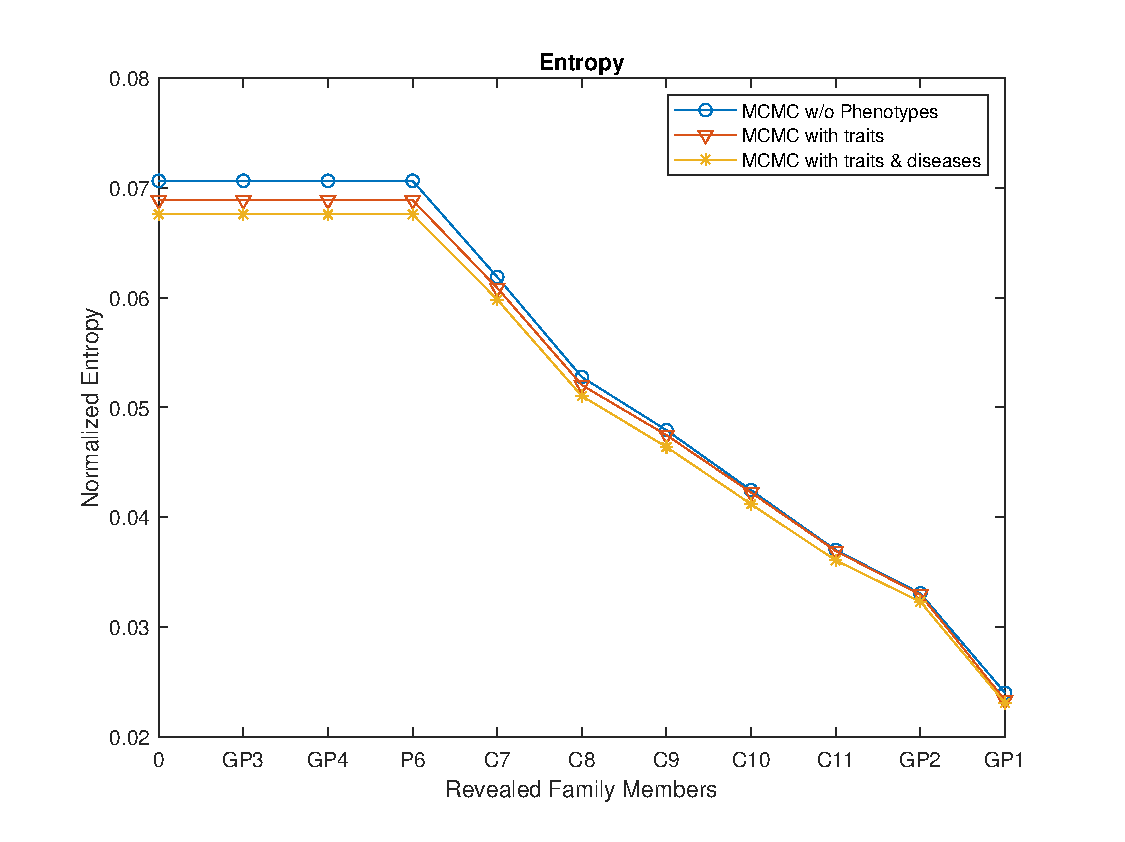
\includegraphics[width=0.8\linewidth]{./figures/P5entropy2.eps}
	\centering
	\caption{附加特征与疾病信息时,攻击者对P5的SNP序列属性隐私推断不确定性降低情况对比}\label{fig:P5entropy2}
\end{figure}


然后,为了考察隐藏的SNP数量对推断攻击模型隐私分析推断能力的影响,我们对家族成员的SNP数据披露顺序与先前实验保持一致,隐藏不同数量的SNP数据后重新进行实验。该实验中,SNP序列被隐藏的比例从50\%变化至10\%,观测攻击者对被攻击者基因序列属性值的推断结果。在图~\ref{fig:P5error3}、图~\ref{fig:P5entropy3}和图~\ref{fig:P5privacyloss3}中,结果表明,随着观测到家族成员的SNP增多,推断攻击的推断能力也随之提高,且这三个指标的结果是一致的。

\begin{figure}[htbp]
	\centering
	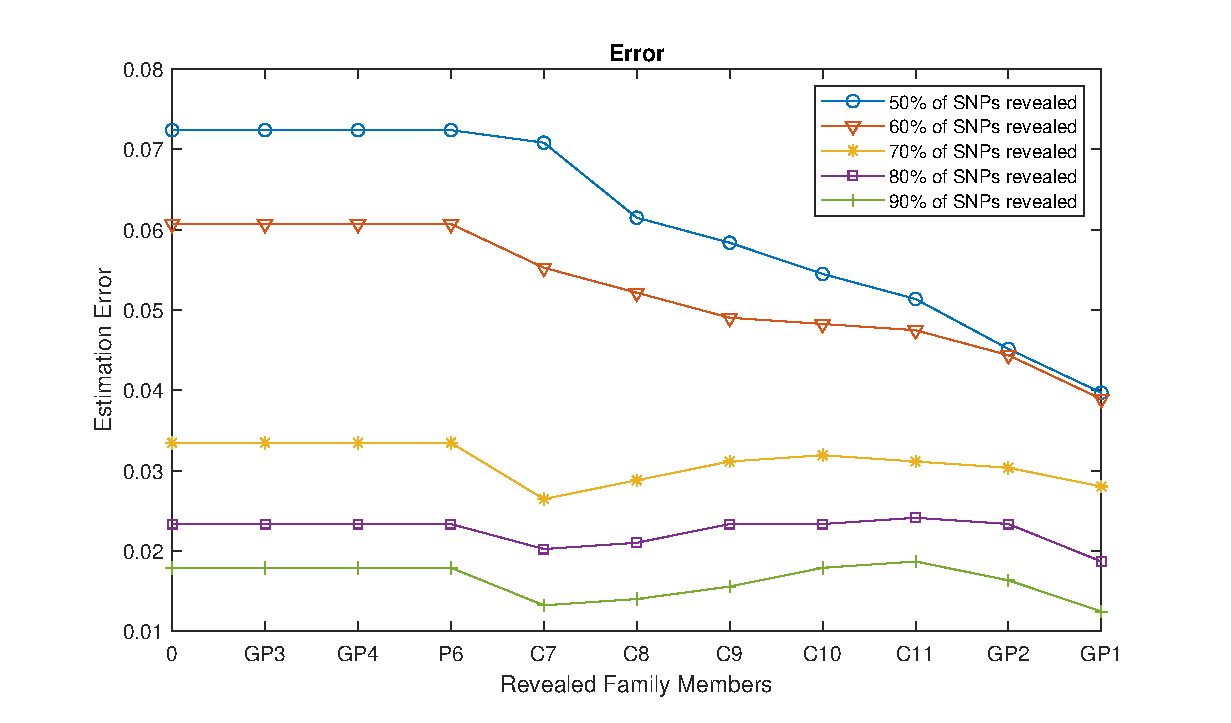
\includegraphics[width=0.8\linewidth]{./figures/P5error3.eps}
	\centering
	\caption{隐藏不同比例SNP序列值时,攻击者对P5的SNP序列属性隐私推断错误率降低情况对比}\label{fig:P5error3}
\end{figure}


\begin{figure}[htbp]
	\centering
	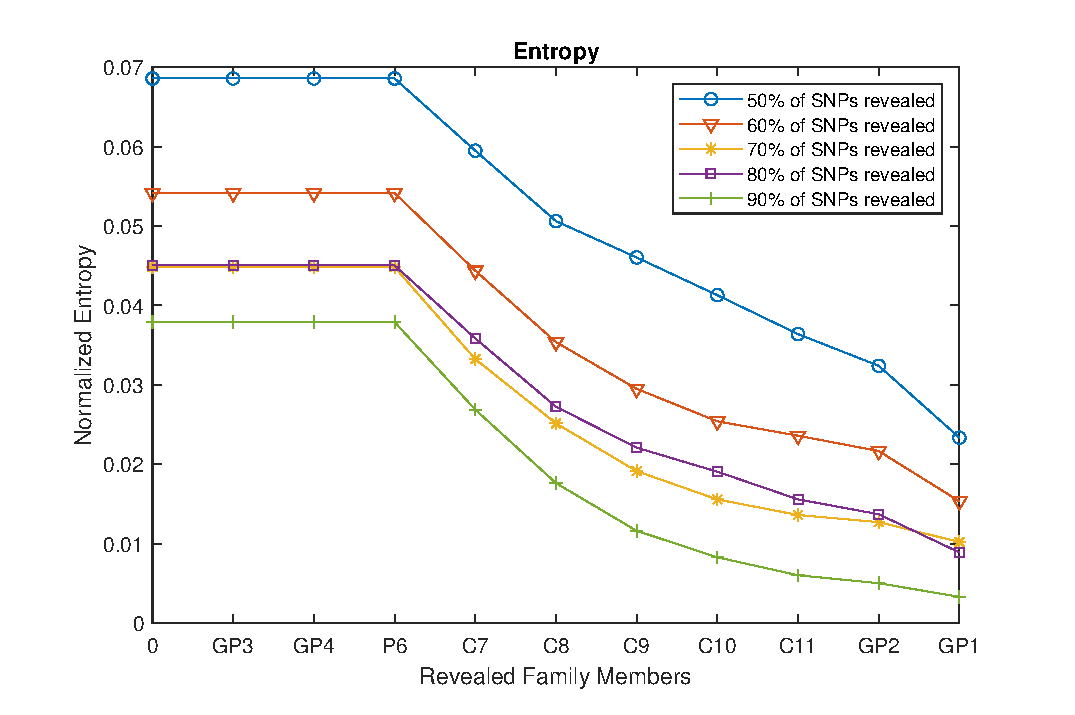
\includegraphics[width=0.8\linewidth]{./figures/P5entropy3.eps}
	\centering
	\caption{隐藏不同比例SNP序列值时,攻击者对P5的SNP序列属性隐私推断不确定性降低情况对比}\label{fig:P5entropy3}
\end{figure}

\begin{figure}[htbp]
	\centering
	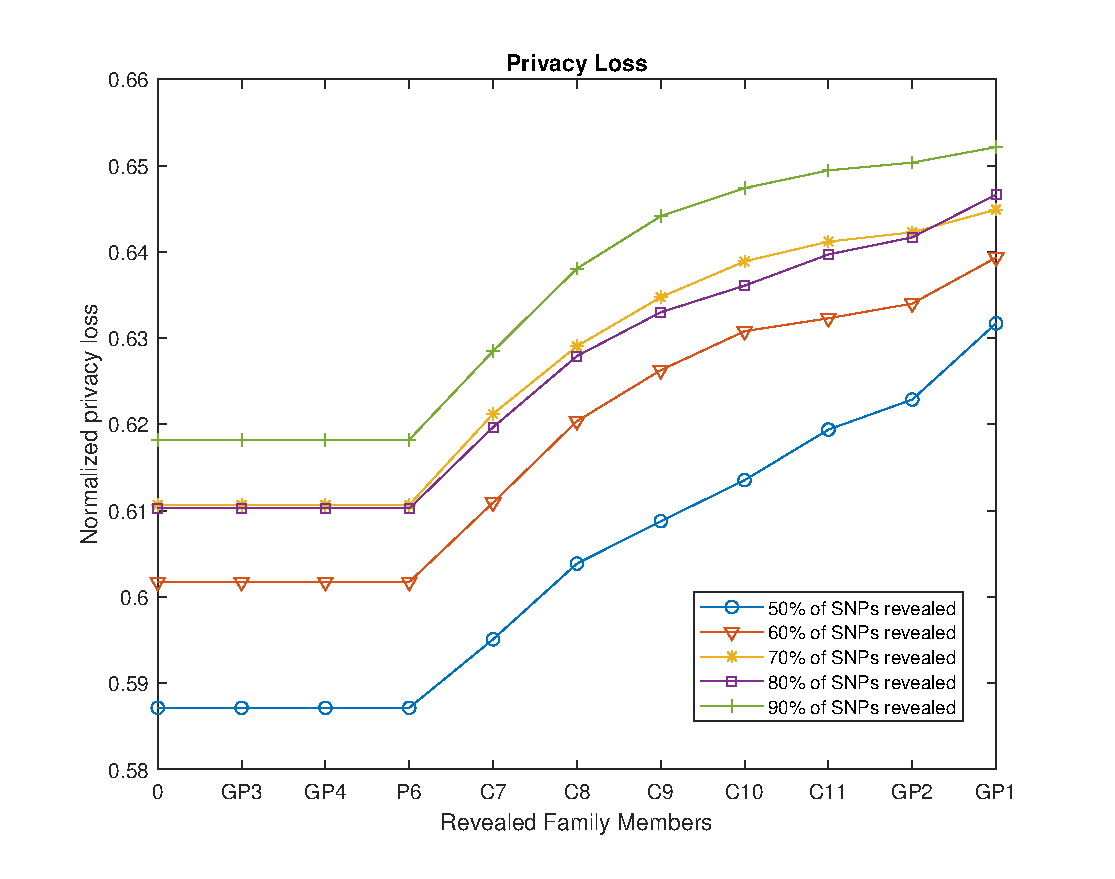
\includegraphics[width=0.8\linewidth]{./figures/P5privacyloss3.eps}
	\centering
	\caption{隐藏不同比例SNP序列值时,攻击者对P5的SNP序列属性隐私推断隐私信息量增加情况对比}\label{fig:P5privacyloss3}
\end{figure}


\textbf{(2) Manuel Corpas家族谱系实验结果}

为了与先前的工作保持一致,本章还使用Manuel Corpas家族谱系数据集进行了实验,并将被攻击者设为母亲(图~\ref{fig:Manuel-Corpas-Family-Pedigree}中的M)。 在此实验中,我们开始从M最亲近的家族成员到最远的家族成员进行披露,并分析所提出的基因序列属性隐私分析推断攻击的强度。实验过程中,假设攻击者观测到部分基因组(50\% SNP序列),SNP相关性状(0.3\% SNP序列) 和疾病 (0.4\% SNP序列)信息,攻击者试图推断母亲的基因组序列属性值隐私。

\begin{figure}[htbp]
	\centering
	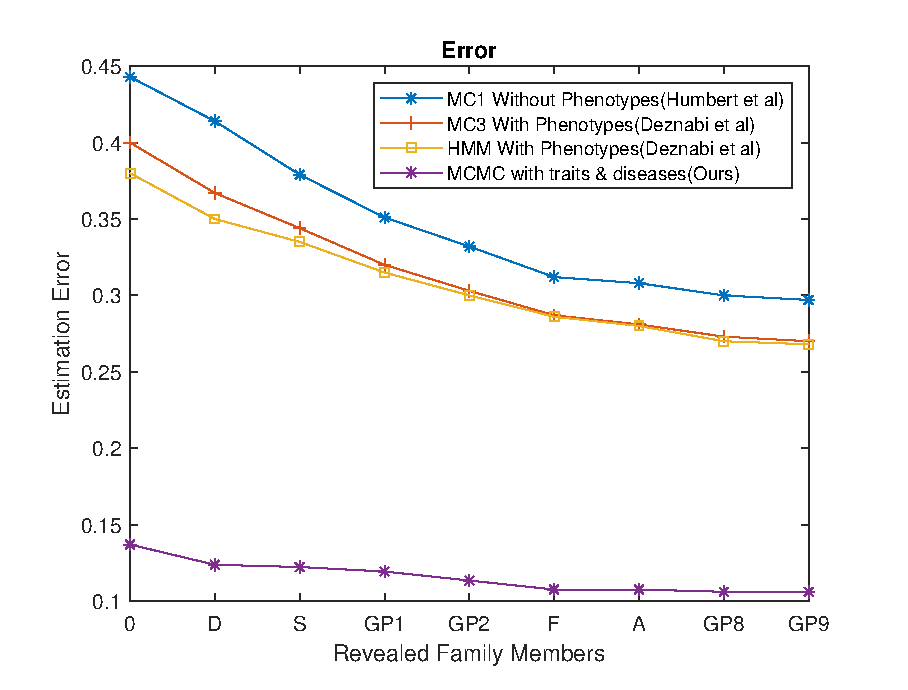
\includegraphics[width=0.8\linewidth]{./figures/Merror1.eps}
	\centering
	\caption{攻击者对M的SNP序列属性隐私推断错误率降低情况对比}\label{fig:Merror1}
\end{figure}



\begin{figure}[htbp]
	\centering
	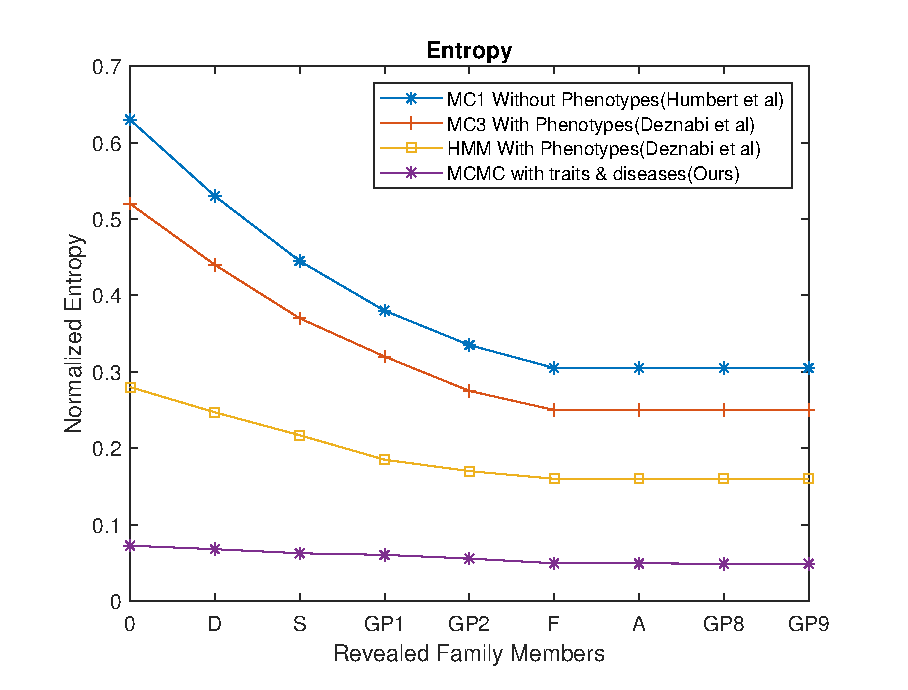
\includegraphics[width=0.8\linewidth]{./figures/Mentropy1.eps}
	\centering
	\caption{攻击者对M的SNP序列属性隐私推断不确定性降低情况对比}\label{fig:Mentropy}
\end{figure}


随机隐藏50\%SNP序列值,先后披露不同家族成员SNP序列数据、相关性状和疾病信息,攻击者对M的SNP序列值属性隐私推断错误,不确定性和不确定性递减(攻击者获得的基因组隐私量)的结果如图~\ref{fig:Merror1},图~\ref{fig:Mentropy}和图~\ref{fig:Mprivacyloss}所示。结果表明,随着披露SNP序列数据的家族成员数量增加,敌手获取的被攻击者基因序列属性隐私越多,我们所提出的隐私分析推断攻击模型比之前的工作有大幅度提高。此外,实验结果与CEPH/Utah Pedigree 1463数据集的实验结果一致。 敌手对基因序列属性隐私推断攻击的强度取决于披露家庭成员的顺序,这与Deznabi等的工作一致。

\begin{figure}[htbp]
	\centering
	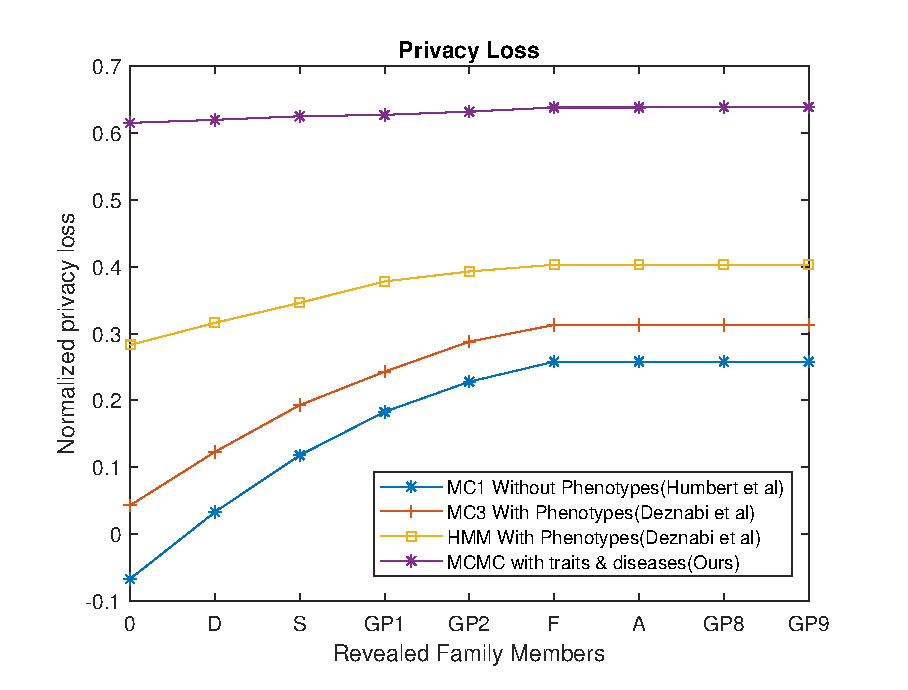
\includegraphics[width=0.8\linewidth]{./figures/Mprivacyloss.eps}
	\centering
	\caption{攻击者对M的SNP序列属性隐私推断隐私量增加情况对比}\label{fig:Mprivacyloss}
\end{figure}

\subsection{方法对比分析}

近年来,有一些针对基因组数据的安全性和隐私问题的工作~\cite{hubaux2017genomic},与本章工作相关的有两类,分别是是基因组插补和两类基因隐私推断分析。

基因型插补在基因组关联研究领域被广泛使用~\cite{marchini2007newa},是指通过统计学方法推断未观测到的基因型值。 基因型插补对在未进行基因型测值的基因标记位评估关联性是非常有用的,且已经有利用不同方法提出的基因型插补模型相继提出~\cite{howie2009flexible,marchini2007newa,howie2014impute2},但是这些工作旨在提高基因组预测的准确性。 我们的工作集中在基因组数据隐私上,试图推断SNP的敏感值并量化个体的基因组属性隐私。


在文献~\cite{samani2015quantifying} 中,作者提出了对(隐藏)Markov链进行单核苷酸多态性的属性隐私推断攻击模型。 本章旨在利用公共信息和观测到的被攻击者的基因组数据推断其自身的基因组隐私。 与文献~\cite{samani2015quantifying}不同,我们试图聚焦在亲属基因组属性隐私问题。 在本章工作中,我们不仅使用了更多的公开基因组信息,例如1000基因组计划数据,孟德尔定律和GWAS目录数据,还使用了被攻击者以外的其他家庭成员的基因组数据。 此外,利用三个隐私度量指标来量化基因组隐私量和推断攻击模型的隐私分析强度。

尽管文献~\cite{humbert2013addressing,humbert2017quantifying}和~\cite{deznabi2018inference}都提出了针对亲属基因组隐私的推断攻击算法,我们与这些工作也存在显着差异,并提高了基因属性隐私推断的准确性。首先,我们针对提出的基因属性隐私推断攻击提出了一个统一的数据模型和敌手模型,该模型可以刻画不同的基因属性隐私推断攻击算法。其次,在先前的工作中使用错误率和不确定性来量化基因组隐私,我们提出了一种基于互信息的基因组隐私量化指标,该指标不仅可以用于量化基因组隐私泄露量,还可以用于度量攻击者的隐私分析能力;第三,我们采用了基于改进隐Markov链的高阶相关性,而不是简单隐Markov链来构建推断攻击模型,且还使用了更多的公共信息来改进推断攻击效果。第四,我们的工作可以用来攻击高密度SNP序列,而先前的方法仅适用于低密度SNP序列。最后,我们的工作从错误率、不确定性以及隐私损失三方面,提高了相互关联的亲属基因组数据属性隐私推断攻击强度。

\section{小结}

本章中,我们针对相互关联的亲属基因序列数据共享场景,提出了一种基因序列数据属性隐私分析推断模型。该模型利用公开基因组数据和观测到的家庭成员的基因组数据进行基因组属性隐私推断攻击。 本章所提出的关联基因序列属性隐私分析推断模型可以应用于高密度基因数据的隐私分析。基于所提出的隐私分析推断模型和算法,攻击者可以高准确率地推断出家族成员中未进行基因数据共享者的SNP序列数据属性值。




	


	

%基于二人博弈的风险访问控制
\chapter{隐私保护风险自适应访问控制模型}
\label{chap:RaBAC-for-privacy}

\textit{ }

\textit{本章针对云环境中涉及隐私或敏感信息数据的共享、应用场景,研究面向隐私保护的风险自适应访问控制模型。在此类以数据为中心的开放跨域环境中,大量用户以不同形式的应用需求来访问数据,数据拥有者(即数据服务提供者或系统)需要动态化、自适应的提供隐私保护。我们在XACML上扩展提出了一种基于风险的自适应访问控制模型,以动态化地在访问控制过程中保护数据隐私,约束隐私侵犯行为,激励诚实访问行为。在该模型中,以Shannon信息论作为工具,在第\ref{chap:entropy-metric-model}章提出的隐私度量模型基础上,提出了基于风险的隐私定义和量化方法;通过风险隐私量化及基于信用卡模型的激励机制,实现访问行为风险阈值的动态调整。对比和分析表明,所提出的模型和方法较现有的工作更加动态化,且实现了隐私保护,易用性更好。
}
\section{概述}
\label{sec:intro}
随着云计算的发展和广泛应用,越来越多的敏感数据和隐私信息在云环境中存储、应用,数据安全和隐私也面临各种挑战。特别是云计算环境中的隐私、机密性和完整性等身份识别与访问控制相关的安全性需要保证。访问控制模型对云安全极为重要,但云环境中仍在大量应用传统访问控制,而这些方案存在不同层面的安全和隐私问题。
传统访问控制模型,例如ACL (访问控制列表) ~\cite{qian2001acla}, RBAC (基于角色的访问控制) ~\cite{jung2012cribac}, ABAC (基于属性的访问控制) ~\cite{zhang2011attribute}和PBAC (基于策略的访问控制) ~\cite{huang2011policy} 是严格和静态的访问控制模型, 需要管理员预定义所有访问策略。 在像云环境这样的“按需共享”的大规模信息系统中,用户和资源都是动态持续变化的,无法预先定义访问策略,而传统的访问控制方法难以适应这种情况。

为了解决此问题,基于风险的访问控制~\cite{ni2010risk,shaikh2012dynamic,wang2011quantified,choi2015framework}被引入,因其将风险级别分析作为授权访问决策的主要输入,以实现动态访问控制。基于风险的访问控制通过考虑访问请求的上下文环境、访问情况和安全策略来评估风险,并根据阈值确定访问权限。这种决定访问权限的方式可以防止由于内部人员滥用数据而导致不必要的隐私信息访问和泄漏,从而实现动态访问控制 ~\cite{chen2011risk}。 因此,风险量化成为基于风险的访问控制中的核心组件。

一般情况下,风险定义为潜在的资源价值损失。在信息系统中,访问风险可以被视为因访问数据所可能造成的潜在泄露信息价值。现有基于风险的访问控制研究提供了不同的方法来确保访问对象的安全性和隐私。Chen等~\cite{cheng2007fuzzy} 提出了一种模糊多级风险访问模型,该模型采用模糊理论来评估访问主体的安全等级和访问客体敏感度等级,随后Ni等~\cite{ni2010risk} 将Chen等的思想扩展为基于模糊推理的访问控制。Wang和Jin~\cite{wang2011quantified} 在健康信息系统的访问控制中提出了一种基于条件熵的风险量化方法,以保护患者的隐私。Shaikh等~\cite{shaikh2012dynamic}提出了一种基于动态风险的访问控制系统决策方法,同时考虑了短期历史访问行为和长期历史访问行为。Khambhammettu等~\cite{khambhammettu2013framework} 在访问请求风险量化中考虑了威胁资源和敌手影响,并以此提出了一个访问控制模型的风险量化方法。Choi等~\cite{choi2015framework} 对上下文信息进行了分类,通过扩展XACML来应用风险,从而通过基于上下文和处理的权限配置文件和规范来估计和应用访问风险。但是这些工作都需要使用相同的方法来对访问主体(用户) 和访问客体 (资源或信息)进行分类,且在大多数场景下很难找到这种方法。尽管现有工作可以动态地基于风险来决定访问许可,但是其最大可容忍风险值 (风险阈值) 是静态的,对于所有用户而言都是相同的容忍度,且缺乏对访问主体的激励机制。

本章针对上述问题,提出了一种基于Markov链和信息熵的风险自适应访问控制模型。首先,为基于风险的访问控制模型定义了一个敌手模型,仅通过比较历史访问行为模式即可对访问请求和用户进行分类。然后,提出了一种基于XACML的风险自适应访问控制框架。在此框架中,添加了策略风险评估组件 (Policy Risk Evaluator Point,PREP),会话控制组件和风险缓解服务组件等三个新组件,并增强了策略执行组件,策略访问组件和策略信息组件等三个标准组件。针对PREP设计了基于类Markov的公式和方法,以根据访问历史行为来计算访问请求的风险值,基于访问请求分类识别来允许/拒绝访问请求,并根据访问历史周期性地计算用户风险,设计激励机制动态调整风险配额和风险消耗配额。

\section{相关工作}
\label{sec:relate}
最近,基于风险访问控制模型吸引了研究人员的注意~\cite{wang2011quantified,shaikh2012dynamic,choi2015framework}。Wang和Jin~\cite{wang2011quantified} 考虑了一种实际的访问控制模型,该模型通过考虑医疗保健的实际情况来保护电子医疗系统中的患者隐私。首先,该模型通过量化与医生数据访问活动相关的风险来做出访问决策。其次,该模型利用医生的整体统计行为和Shannon条件熵来量化侵犯隐私的风险。Hui等~\cite{hui2015risk}对此模型进行了改进,但是两个模型都不能在近期历史和旧历史之间取得平衡,也没有采取任何措施来减轻高风险。Shaikh等~\cite{shaikh2012dynamic} 提出了一个用于访问控制系统的基于动态风险决策方法。首先,其改进了标准XACML框架,添加了策略风险和信任评估者组件。其次,系统根据奖励和惩罚历史来计算访问主体的信任值和访问客体的风险值。此外,该系统通过使用基于指数加权移动平均值 (EWMA) 的方法来考虑短期访问历史和长期访问历史的不同影响。 最后,分析了允许非法访问和限制合法访问的威胁。该系统可以根据过去的行为自适应并适度增加或减少所有用户对资源的访问权限,但是访问主体和访问客体需要相同的分类方式进行标记。此外,该系统仅根据主体-客体间奖励或惩罚点做出访问决策,没有针对访问主体历史行为的奖励机制或惩罚机制。Choi 等~\cite{choi2015framework}  提出了一种适用于医疗信息系统的基于风险的访问控制框架,以保护患者的敏感数据和隐私。该方法的主要思想是根据医疗情况的严重性,通过动态访问授权决策来估计和应用访问风险。在对有关医生的目的、患者状况、治疗方案以及医疗数据的上下文信息进行分类之后,可以根据特定患者状况和治疗方案条件下访问请求与目的之间的相关性来评估风险等级。尽管该模型可以在某些严重情况下授权访问权限,但其并未提供缓解高访问风险的措施,使得在后续访问过程中造成风险量化混乱。

我们提出的方法与~\cite{wang2011quantified,shaikh2012dynamic,choi2015framework}等文献的方法相比,具有以下新的特性:

\begin{enumerate}
	\item 该方法中,资源所有者或访问控制系统管理员仅需根据访问客体的属性和需求,通过某些标准方法(如用于医疗记录分类的IDC-10) 或定制方法来标记或分类访问客体(如信息资源,存储记录或数据等),不需要为访问主体 (如经过身份验证的用户) 特定明确的角色或工作职责,也无需为每个访问请求设定特定目的。
	\item 利用访问主体的历史访问数据,通过数据聚类识别访问主体的工作职责,且将访问主体划分为不同的非相交组。
	\item 基于类Markov模型设计了访问请求风险值计算、用户风险值计算、不同组中的用户迁移等方法。
	\item 设计了一种类似于信用卡模型的激励机制,对主体的所有访问行为进行监督,并通过这种机制约束了风险请求和风险用户。
\end{enumerate}

\section{基本定义和敌手模型构建}
\label{sec:adversary_model}

本节进行若干假设和定义,并此提出基于风险访问控制模型的敌手模型。如第~\ref{sec:intro}节所述,本章主要面向在数据共享应用场景中,经过对身份验证的用户访问行为控制以保护共享数据隐私。在此类系统中,所有用户,包括敌手,都被授权使用存储的数据,本章的目的是防止用户不履行其在系统中的职责时,访问不该访问的敏感或隐私数据而造成的隐私泄露。

\begin{assumption}
	\label{ass:user_obligations}
	所有通过身份验证的用户都将履行其职责。
\end{assumption}

若用户通过了特定信息系统的身份认证,则其为合法用户,且有责任履行其工作职责。在系统中,若用户长期不履行工作职责,系统将不会容忍该用户,这样即使用户未履行其工作职责,也不会不会对敏感或隐私数据造成太大伤害。 根据假设 ~\ref{ass:user_obligations},可以将经过身份验证的用户分为几类,即\emph{诚实用户}和\emph{好奇用户}, 有时将\emph{好奇用户} 认为是 \emph{恶意用户}。 \emph{诚实用户} 仅访问其职责所需的数据或信息,  \emph{好奇用户} 除了具有与\emph{诚实用户}相同的访问行为,其有时会故意或随机访问与其职责无关的敏感或隐私数据。 只有当\emph{好奇用户}故意访问与工作职责无关的敏感或隐私数据或信息时,其才被称为 \emph{恶意用户}。方便起见,在本章研究对这两个概念并不区别对待。

\begin{assumption}
	\label{ass:honest_user}
	大多数通过身份验证的用户都是诚实用户。 相应地,只有一部分经过身份验证的用户是好奇用户或恶意用户。
\end{assumption}

假设~\ref{ass:honest_user}在现实环境中是合理的。 现实中的大多数人都是好人,否则我们的社会将会混乱。假定部署在云或本地设备中的任何信息系统都有序运行,且大多数用户都是诚实的。一旦\emph{好奇用户}被系统识别出来,可以通过惩罚或拒绝好奇用户的访问请求来确保这一假设一直成立。

对于某一经过身份认证的用户,可以根据访问请求的风险值将其访问行为分为两类。 一部分行为具有较高的风险值,而另一部分行为具有较低的风险值。 该分类由以下事实决定:没有绝对的分类,即所存储的信息和数据中哪些与该用户的职责有关,哪些与该用户的职责无关。 我们的目的是将 \emph{好奇用户} 与\emph{诚实用户}区分开, 拒绝 \emph{好奇用户}访问请求,并减少\emph{诚实用户}的偶然高风险行为对\emph{诚实用户}的访问控制决策的影响。为了实现该目标,需实现以下内容:

\begin{enumerate}
	\item 根据身份验证用户的工作职责将其分为不同的用户组,且每两个组的交集在一段时间内为空;
	\item 识别出每个用户的职责变化,并将变化后的用户分别分类到适当的用户组;
	\item 评估每个用户的每个访问请求的风险,并识别出具有高风险值的访问请求;
	\item 定期评估每个用户的风险,识别出好奇用户并拒绝其访问请求。
\end{enumerate}

由前文可知,同一组中的所有用户都具有相似的工作职责,因此,若 ~$u \in g$~,则不区分用户 ~$u$~ 和用户组 ~$g$~ 的职责;在提出的敌手模型中,对于某一用户组中用户的访问请求,若该访问请求的访问数据蕴含隐私信息比其历史访问的隐私信息更多,则该访问行为具有高风险。为了对高风险请求和正常请求的风险计算进行建模,这里引入两个函数,即 ~$sr$~ \emph{自我风险函数}和~$gr$~ \emph{组风险函数}。 其中,~$sr(u,q)$~ 表示用户 ~$u$~的当前访问请求 ~$q$~ 相对于 ~$u$~自身的历史访问行为的风险值, ~$gr(u,q)$~ 表示用户~$u$~当前访问请求~$q$~相对于~$u$~所属用户组 ~$g$~ 历史访问行为的风险值。~$sr(u,q)$~ 和 ~$gr(u,q)$~ 的具体计算公式将在 ~\ref{sec:proposed model}中讨论。

\begin{definition}%[Self Risky Request and Self Normal Request]
	\label{def_self_risky}
	令 ~$sr(u, q_0), sr(u, q_1), sr(u, q_2), ... ,sr(u, q_{n-1})$~ 为~$u$~ 过去 ~$n$~ 次访问请求的自风险值, ~$sr(u,q)$~ 为 ~$u$~ 当前 (第~$n$~次) 请求 ~$q$~ 的风险值,令 ~$\epsilon_s \in (0,1)$~ 为分位数。若~$sr(u,q) \geq  (1+\epsilon_s) / n  \sum ^{n-1}_{i=0}{sr(u,q_i)}$~,则访问请求 ~$q$~ 是一个\textbf{用户自风险请求}。否则, ~$q$~ 是一个 \textbf{用户自我正常请求}。
\end{definition}

\begin{definition}%[Group Risky Request and Group Normal Request]
	\label{def_group_risky}
	令 ~$gr(\cdot, q_0), gr(\cdot, q_1), gr(\cdot, q_2), ... , gr(\cdot, q_{m-1})$~ 是用户 ~$u$~ 所属用户组中所有用户过去 ~$m$~ 访问请求的风险值, ~$gr(u,q)$~ 为用户 ~$u$~ 的当前访问请求 ~$q$~  ( ~$u$~ 所属组的第~$m$~次访问请求 )。 令 ~$\epsilon_g \in (0,1)$~ 为分位数。若~$gr(u,q) \geq  (1+\epsilon_g) / m  \sum ^{m-1}_{i=0}{sr(\cdot,q_i)}$~,则 ~$u$~ 的访问请求 ~$q$~ 是一个\textbf{组风险请求}。否则, ~$u$~ 的 ~$q$~ 是一个 \textbf{组正常请求}。
\end{definition}


上述定义 ~\ref{def_self_risky}和定义~\ref{def_group_risky} 都基于Markov模型,且可以根据访问控制系统需求自动确定Markov链的长度。 此外,两个长度都可以随时间变化。通过这两个定义可以有效识别访问控制系统的高风险访问请求。具体详细计算方法,将在第~\ref{sec:proposed model}节中详细讨论。 在一个时间周期内,特定组的每个用户的访问请求数据的期望服从某些分布,而该组的所有用户请求的数据的期望也服从一定的分布。根据假设 ~\ref{ass:honest_user},若 ~$u$~ 是一个诚实的用户,则用户 ~$u$~ 的访问数据的分布 ~$D_u$~ 与同一组中所有用户访问的数据的分布 ~$D_g$~ 密切相关。相反,若 ~$u$~ 是一个好奇的用户,则 ~$D_u$~ 与 ~$D_g$~ 相关性低。 为了有效描述这种关系, 引入 \emph{相关关系函数} ~$\theta$~ 并将在 第~\ref{sec:proposed model}节中进行讨论。对于用户 ~$u$~ 在组 ~$g$~ 中通过请求 ~$q$~ 访问的数据集合 ~$r$~,~$\theta_g (r_q,u))$~ 返回一个~[0,1]~的实数,该实数反映 ~$r_q$~ 和 ~$u$~ 的职责之间的相关程度,~$\theta_g (r_q,u))$~ 越高, 风险~$r_q$~ 对于用户 ~$u$~ 的职责而言就越高。


\begin{definition}%[Honest User and Curious User]
	\label{def_curious user}
	假定 ~$D_g$~ 是特定组 ~$g$~ 的所有用户 ~$u_g$~ 访问的数据数据集合 ~$R_g$~ 的先验概率分布,~$D_g$~ 使得 ~$pr(R_i)=\delta \cdot \theta_g (\cdot,u_i))$~,其中 ~$u_i$~ 是 ~$g$~ 中的用户, ~$r_i$~ 是 ~$u_i \in g$~ 访问的数据数据集合,而 ~$\delta$~ 是实数,因此 ~$\Sigma_{u_i \in g}Pr(R_i) = 1$~。
	\begin{itemize}
		\item \textbf{诚实用户}: 设 ~$r_i$~ 为 ~$u_i \in g$~ (即诚实用户) 在过去一个周期内访问的数据集,每个数据记录 ~$r_k \in R_i$~,以概率 ~$(1-\epsilon_1)$~ 服从 分布~$D_g$~,以概率 ~$\epsilon_1$~ 服从~$r_g$~ 所有可用数据的均匀分布, 其中 ~$\epsilon_1 \in [0,1]$~。
		\item \textbf{好奇用户}: 设 ~$r_i'$~ 是 ~$u_i' \in g$~ (即好奇用户) 在过去一个周期内访问的数据集,对于每个数据 ~$r_k' \in R_i'$~,以概率 ~$(1-\epsilon_1)(1-\epsilon_2)$~ 服从分布 ~$D_g$~ ;以概率 ~$\epsilon_1 (1 - \epsilon_2)+ \epsilon_2$~服从~$r_g$~ 所有可用数据的均匀分布,其中 ~$\epsilon_1, \epsilon_2 \in [0,1]$~。
	\end{itemize}
\end{definition}

如定义~\ref{def_curious user} 所述, 诚实用户的数据访问始终遵守其职责 (即用户访问总是服从分布~$D_g$~), 例外情况的发生概率小于 ~$\epsilon_1$~。相反,好奇用户的行为与诚实用户的行为以概率~$1-\epsilon_2$~ 相同,其履行了自己的职责;好奇用户以概率 ~$\epsilon_2$~ 过度访问敏感数据。在真实场景中,~$\epsilon_1$~ 和 ~$\epsilon_2$~ 的值都较小。

\section{风险自适应访问控制模型}
\label{sec:proposed model}
本节根据可扩展访问控制标记语言 (XACML) ~\cite{verma2004xml} 改进提出一个风险自适应访问控制模型,然后提出如何初始化访问控制系统,如何定义并量化访问请求风险、如何为请求做出访问决策、访问控制详细过程、如何动态识别好奇用户,以及如何设计激励机制等具体方法。

\subsection{风险访问控制框架}
\label{subsec:framework}

在标准XACML框架中,一旦策略决策组件(PDP) 收到了来自访问主体 (即访问控制系统的用户) 的访问请求, 其首先会从策略访问组件 (PAP) 和策略信息组件 (PIP) 然后决定接受还是拒绝该请求。 此外,策略执行组件 (PEP) 难以处理与请求者的交互,策略访问组件 (PAP) 是静态的,且职责服务和策略信息组件 (PIP) 都缺乏风险管理。
在我们提出的框架中,除了对PEP,PIP和PAP进行了增强,还新增了三个组件,即策略风险评估组件 (PREP),会话控制和风险缓解服务 (嵌入在职责服务的组件中)。 在该框架中,一旦PDP收到来自经过身份验证的用户的访问请求,且在做出决定之前,它会请求与特定访问主体 (即正在请求访问的用户) 和其历史访问数据相关的风险值。此外,在做出访问控制决策后,一些反馈信息将提供给职责服务组件。 所提出的风险自适应访问控制模型的流程如图~\ref{fig:Process_flow}所示。 该框架是基于标准可扩展访问控制标记语言 (XACML) 提出的,与文献~\cite{shaikh2012dynamic}的框架有所不同,所提出框架的所有新组件均以虚线标记,所有增强的组件均浅灰色标记。


\begin{figure}[htbp]
	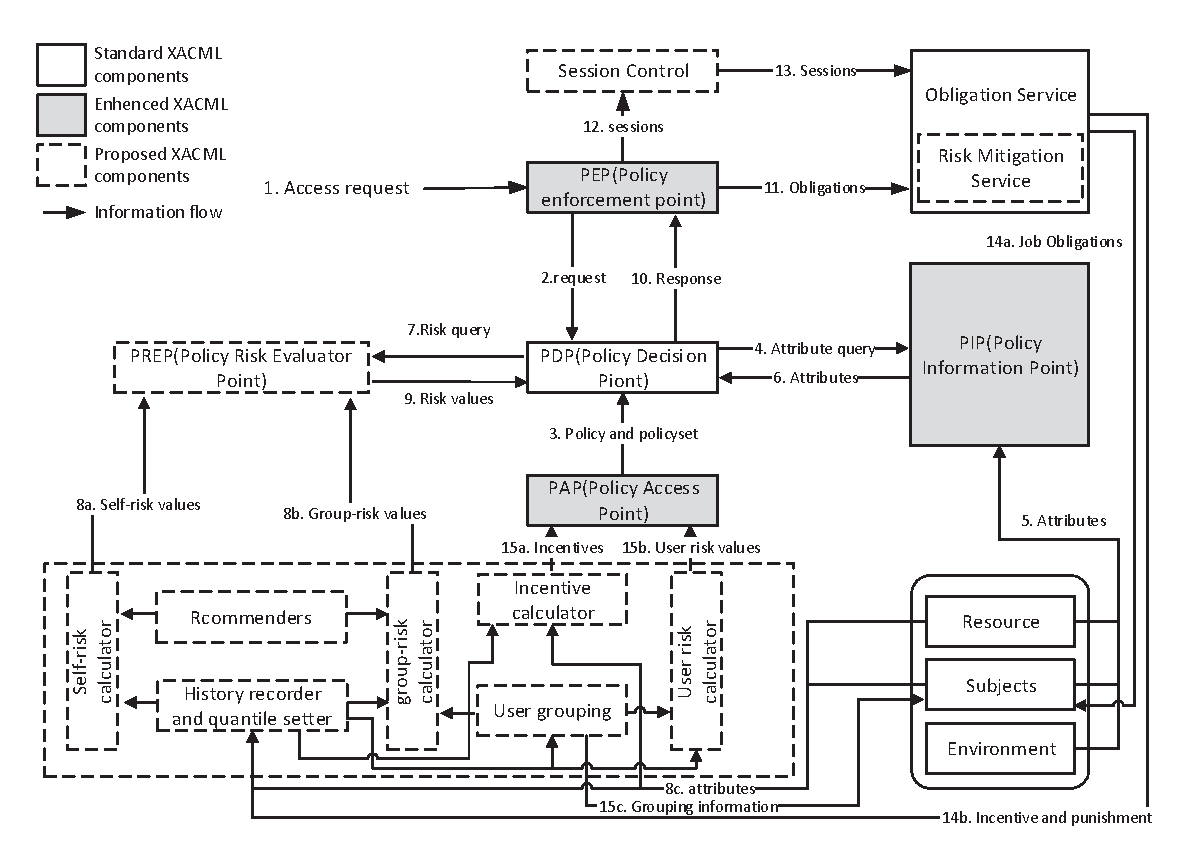
\includegraphics[width=\linewidth]{./figures/Process_flow.eps}
	\caption{基于XACML的风险自适应访问控制框架流程}
	\label{fig:Process_flow}
\end{figure}

在所提出的基于标准XACML风险访问控制框架中,所有访问请求均由经过身份验证的用户发送,我们称此类用户为访问主体。 从步骤1到步骤6,其过程类似于Shaikh等~\cite{shaikh2012dynamic} 和Verma ~\cite{verma2004xml}所述的过程。一旦收到所有必需的信息,PDP就将有关当前请求的风险查询发送到PREP (步骤7)。 PREP根据用户的过去行为和历史行为的风险值来评估风险值 (步骤 8)。 每个请求都有两个风险值,一个是根据当前用户自己的过去行为评估的自我风险值,另一个是根据所有用户的过去行为以及当前用户属于同一组所有用户评估的群组风险值。
若系统没有足够的历史数据,则PREP将根据系统平均风险水平计算两个隐私风险值。与该访问请求相关的当前风险值将返回到PDP (步骤 9)。根据风险值,PDP做出访问控制决策,并将此决策转发给PEP,由PEP执行 (步骤10)。无论是允许访问还是拒绝访问,PEP都会通知 (步骤 11) 职责服务组件,该组件将决定是否需要风险缓解服务。在访问请求执行的延迟时间内,会话控制组件监视请求者的行为,并管理访问会话 (步骤 12)。若在该会话中访问行为的隐私风险太高,则会话控制通知职责服务组件并控制该会话中的请求 (例如,终止会话) (步骤 13)。 职责服务将决定是激励还是惩罚用户,并更新主体的属性 (例如工作职责) (步骤 14)。 PREP定期通过激励机制重新分配预算配额,重新将用户标识为正常用户或有风险的用户,并将用户分类到为更合适的用户群组中(步骤 15)。

\subsection{自适应风险机制}
\label{subsec:risk values and decision}

\textbf{(1) 自适应访问风险计算}

本章中,动态评估访问请求风险值的方法是根据请求者的历史访问行为以及请求者所属组的所有成员而设计的。对于特定的用户组,该组中的每个用户都按照相似的工作职责划分到该组中,其工作职责在短时间段内相对稳定,且会在长时间周期范围自然演变。对于特定的用户,其所属的组可能会随时间而改变。因此,应该根据用户本人和组的短时间访问行为特征来评估特定组中用户的访问请求风险,可以根据用户本人和组的长期历史访问行为特征来计算用户风险。本节仅关注对特定用户的访问请求隐私风险评估。直观地,若一访问请求的目的是访问一个时间周期内没有被访问过的数据数据集,则即使该数据数据集在以前被该用户访问过,该请求的访问请求的隐私风险值也很高。我们将该思想应用于对访问请求的隐私风险评估中,基于信息论相关概念,并对其进行改进,以设计本章用以进行访问请求隐私风险值量化的函数。

令 ~$u \in u$~ 是已认证用户集 ~$u$~, 且 ~$u$~ 属于用户组 ~$g$~ ,该用户组~$g$~ 是 ~$u$~ 的子集。 如定义 ~\ref{def_self_risky} 和 ~\ref{def_group_risky}所述,~$u$~ 的请求 ~$q$~ 有一定的隐私风险,表示为 \emph{用户自风险} ~$sr$~ 和 \emph{组风险} ~$gr$~ 。

令 ~$(q_1, q_2, ... , q_{n-2}, q_{n-1})$~ 为用户~$u$~的前~$n-1$~次访问请求,而 ~${r_1, r_2, ... , r_{n-2}, r_{n-1}}$~ 分别为这些请求的访问数据集。 令 ~$q_n$~ 是用户当前的访问请求,该访问请求所要访问的数据集为 ~$r_n$~。若将每个访问请求和访问数据集对 ~$(q_n,r_n)$~ 视为随机事件,则该对 ~$(q_i,r_i)$~ 的信息量可以通过\textbf{自信息}表示。则当前访问请求的访问隐私自风险 ~$sr$~ 可表示为

\begin{equation}
\label{eq:self risk}
sr(u,q_n)=I(q_n,r_n)
\end{equation}

由公式~\ref{eq:self risk} 中可知, 可由~$r_n$~ 中预期访问的数据集的概率分布计算得到~$rs$~。此外,由于不同的数据集具有相同的标签,因此其可能具有相同的敏感信息。 故而,在不同的情况下应使用不同的分类方法对数据进行标签化分类。 可以将关系数据库中的数据分类为相同的数据,以使这些数据具有相同的信息量;在电子医疗信息系统中,具有相同信息的医疗数据应按标签分类 (如ICD-9或 ICD-10代码)。

为方便起见,后文将不再对访问请求 ~$q$~ 和其预期访问的数据集 ~$r$~ 进行区分, 即,每个不同的访问请求都试图访问具有不同信息的不同数据。 假设访问请求集 ~$q_u$~ 中有 ~$k$~ 个不同的请求 ~$q_1,q_1,....,q_k$~ ,其中包括前~$n-1$~ 次访问请求和 ~$u$~ 的当前访问请求 ~$q_n$~ ,以及概率分别为 ~$p_1,p_2,...,p_k$~ 。 若在 ~$k$~ 个不同的请求中 ~$q_n$~ 与 ~$q_i$~ 相同,则方程 ~\ref{eq:self risk} 可以简化为

\begin{equation}
\label{eq:self risk 2}
sr(u,q_n)=I(q_i)=-logp_i
\end{equation}

公式 ~\ref{eq:self risk} 和 ~\ref{eq:self risk 2} 都在具有足够的历史访问请求行为时,才对用户~$u$~ 有效,若无有足够的历史访问行为历史供 ~$u$~进行计算, 则可以使用某个默认值 (例如1) 或整个历史数据。
	\begin{equation}
	\label{eq:self risk 3}
	sr(u,q_n)=
	\left\{
	\begin{array}{ll}
	I(q_i)=-logp_i, & \hbox{是否有足够的历史数据;} \\
	Avg(I(u,q)), & \hbox{若历史还不够;} \\
	1, & \hbox{若没有可用的历史数据。}
	\end{array}
	\right.
	\end{equation}

由公式~\ref{eq:self risk 3}可知,~$rs$~ 的计算依赖于用户 ~$u$~ 自己过去 ~$n-1$~ 次访问行为的Markov链,且Markov链的长度可以根据需要针对每个用户进行动态和个性化设置。这样,可以通过调整参数~$n$~的大小,适当地平衡用户 ~$u$~ 的短期历史和长期历史行为对隐私风险值的影响。

令 ~$sr(u, q_1), sr(u, q_2), ... , sr(u, q_{n-2}), sr(u, q_{n-1})$~ 为过去 ~$n-1$~ 次允许请求 ~$u$~ 的隐私自风险值,并令 ~$sr(u,q)$~ 为 ~$u$~ 当前 (第n次) 请求 ~$q$~ 的隐私自风险值。令 ~$\epsilon_s \in (0,1)$~ 为分位数, 通过定义 ~\ref{def_self_risky} 可以方便地将~$q$~ 定义为 \textbf{自风险请求} 或 \textbf{自正常请求} 。

类似地,可以通过该Markov方法得到当前用户 ~$u$~ 的当前访问请求的组风险值。 令 ~$q_1,q_1,....,q_l$~ 是访问请求集 ~$q_g$~ 中的元素,它表示组 ~$g$~ 过去的 ~$m-1$~ 次允许访问请求和 ~$u\in g$~ 的当前访问请求 ~$q_m$~, ~$p_1,p_2,...,p_l$~ 分别为历史访问请求数据集的标签化概率分布。 若 ~$q_m$~ 与 ~$q_g$~ 中的 ~$q_i$~ 相同, 则 ~$gr(g,q_m)$~ 可计算为
	\begin{equation}
	\label{eq:group risk}
	gr(g,q_m)=
	\left\{
	\begin{array}{ll}
	I(q_i)=-logp_i, & \hbox{若有足够的历史数据 ;} \\
	Avg(I(g,q)), & \hbox{若历史数据不够;} \\
	1, & \hbox{若没有可用的历史数据。}
	\end{array}
	\right.
	\end{equation}
类似地,通过定义 ~\ref{def_group_risky} 可将 ~$u\in g$~ 的访问请求 ~$q$~ 识别为 \textbf{组风险请求}或\textbf{组正常请求} 。

\textbf{(2) 动态访问控制决策方法}

自风险值 ~$sr(u,q)$~ 和组风险值 ~$gr(g,q)$~ 都是访问决策的基础。 根据定义 ~\ref{def_self_risky} 和 定义~\ref{def_group_risky}, 可将所有用户的访问请求分为四类,即访问请求 ~$q$~ 有四个不同的风险级别。故,数据服务提供者或系统可以根据请求的风险级别做出访问控制决策,即
\begin{equation}
	\label{eq:decision}
	decision=
	\left\{
	\begin{array}{ll}
	p, & \hbox{若~$q$~为自正常访问请求,且为群组正常访问请求;} \\
	p(rm), & \hbox{若~$q$~为自风险访问请求,但为群组正常访问请求;} \\
	d, & \hbox{若~$q$~为自风险访问请求,且为群组风险访问请求;} \\
	d(p), & \hbox{若~$q$~为自正常访问请求,但为群组风险访问请求。} \\
	\end{array}
	\right.
\end{equation}
其中,~$p$~表示因为访问请求时正常的,访问请求没有隐私风险,授权该访问请求;~$p(rm)$~ 表示该访问请求隐私风险较低,用户通过一定风险消减措施之后,可以授权该请求进行数据访问;~$d$~ 表示由于该访问请求隐私风险过高而拒绝访问;~$d(p)$~ 表示该访问请求隐私风险太高,应当惩罚并限制用户访问包含隐私的敏感数据集。

公式~\ref{eq:decision}中对访问请求的访问控制决策的确定基于以下原因。 若请求既是自身正常请求又是组正常请求,则用户和组在过去一段时间内频繁访问该访问请求的请求访问数据集,因此该请求是正常的而且没有风险。 若某个请求是自风险请求,且是组正常请求,则表示该组中的其他用户(非用户本人)经常访问了预期数据,这些数据与该组的工作职责相关,但用户几乎不访问,且对该用户的访问风险很小,应该在系统采取某些适当的风险缓解措施后授权访问权限。若某个请求是自风险请求,且是组风险请求,则该组几乎不会访问预期数据,这些数据与该组的工作职责无关,因此访问请求应被拒绝。若某请求是一个自正常请求,且是一个组风险请求,则该组几乎不会访问预期数据,且这些数据与该组的工作职责无关,但该用户已多次访问数据,因此应拒绝访问此请求,并要加重惩罚以限制该用户访问。


\subsection{激励机制设计}
\label{subsec:User classification and incentive mechanism}

本节首先基于用户和用户组历史访问请求,提出可定期地将用户 ~$u \in g$~ 识别为好奇用户还是诚实用户的方法。然后,提出可定期确定用户如何从一个组迁移到另一个组的方法; 最后,设计了一种激励机制,以监督用户访问行为,抑制风险请求和风险用户。特别地,本节的所有方法,都基于类Markov模型和信息论。

\textbf{(1) 用户风险值计算}

对于特定用户组中的用户,可在假设 ~\ref{ass:user_obligations}和假设 ~\ref{ass:honest_user} 下通过定义 ~\ref{def_curious user} 将用户识别为好奇用户或诚实用户。但实际上很难找到 ~$\theta_g$~ 的特定函数,我们通过使用组 ~$g$~ 的访问模式来近似刻画函数 ~$\theta_g$~ 。信息熵可用来表示信息集的不确定性,故而我们采用Shannon熵来表示组和用户的访问模式,用户访问行为的熵越高,用户越好奇。

令 ~$T$~ 为周期时间,~$q_{g,T}=(q_1, q_2,...,q_{s_g})$~ 为 ~$T$~ 中 ~$u$~ 组所有用户的访问请求, ~$q_{g,T}$~ 服从分布
~$p(g,T)=
(
\begin{array}{l}
q_{g,1},  q_{g,2}, ...,q_{g,n_g}\\
p_{g,1},  p_{g,2}, ...,p_{g,n_g}\\
\end{array}
)
~$~。令 ~$q_{u,T}=(q_1, q_2,...,q_{s_u})$~ 为 时间~$T$~ 中来自用户 ~$u \in g$~ 的访问请求, ~$q_{u,T}$~ 服从分布
~$p(u,T)=
(
\begin{array}{l}
q_{u,1},  q_{u,2}, ...,q_{u,n_u}\\
p_{u,1},  p_{u,2}, ...,p_{u,n_u}\\
\end{array}
)
~$~。

然后可以计算出用户 ~$u \in g$~ 在时间段 ~$T$~ 中的风险值 ~$risk(u,T)$~ 为
\begin{equation}\label{eq:user risk}
risk(u,T)=max \{\frac{H(P(u,T))-H(P(g,T))}{H(P(g,T))},0\}
\end{equation}
其中,公式 ~\ref{eq:user risk}表示在过去的时间段 ~$T$~ 中,用户风险随熵的增加而线性增加。但实际上,始终存在阈值 ~$\phi$~, 使得用户A和用户B的风险相似, 当 ~$H(P(A,T))>H(P(B,T))>\phi$~ 时,甚至 ~$H(P(A,T))-H(P(B,T))$~ 非常大。然后可以将公式 ~\ref{eq:user risk} 中的风险值计算改进为
\begin{equation}\label{eq:user risk 2}
risk'(u,T)=\alpha ^ {max \{H(P(u,T))-H(P(g,T)),0\}}
\end{equation}
其中, ~$\alpha \in (0,1)$~, 而风险的结果 ~$risk'(u,T)$~ 将是 ~$~[\alpha, 1)$~ 中的实数。 公式~\ref{eq:user risk 2} 中所述函数是平滑的,在实际场景中更合适。

\textbf{(2) 用户类型识别}

一个用户 ~$u \in g$~ 可以由过去一段时间 ~$T$~中的风险值 ~$risk(u,T)$~ 或 ~$risk'(u,T)$~ 来标识。 若 ~$risk(u,T) > 0$~ 或 ~$risk'(u,T)>\alpha$~, 我们称 ~$u$~ 在过去一段时间 ~$T$~ 中是好奇用户, 我们称 ~$u$~ 为诚实用户,前提是  ~$risk(u,T) = 0$~ 或 ~$risk'(u,T)=\alpha$~。形式上,

\begin{equation}\label{eq:user type}
type(u,T)=
\left\{
\begin{array}{ll}
c, & \hbox{iff ~$risk(u,T) > 0$~ or ~$risk'(u,T)>\alpha$~;} \\
h, & \hbox{iff  ~$risk(u,T) = 0$~ or ~$risk'(u,T)=\alpha$~.} \\
\end{array}
\right.
\end{equation}

公式~\ref{eq:user type} 为一个周期时间内的用户分类提供了基础,但是我们并不总是在短时间内将一个人分类为好人还是坏人。 实际上,在某些情况下我们需要对一个人进行长时间的调查,这里我们对用户 ~$u \in g$~ 的风险值进行多次评估,然后形成 ~$u$~ 的用户隐私风险值链。设 ~$T_n$~ 为当前期间,~$T_0, T_1, T_2, ..., T_{n-1}$~ 为过去 ~$n$~ 个时间周期,~$n$~ 个时间周期中,用户 ~$u \in g$~ 的用户风险值可分别通过 ~$risk(u,T_0),risk(u,T_1),risk(u,T_2),..., risk(u,T_{n-1})$~ (or ~$risk'(u,T_0), risk'(u,T_1), risk'(u,T_2), ..., risk'(u,T_{n-1})$~)分别计算得到。因此,可根据过去的 ~$n$~ 个风险值 ~$u$~ 来识别当前期间的用户类型是诚实用户还是好奇用户,即
\begin{equation}\label{eq:user type Tn 1}
type(u,T(n))=
\left\{
\begin{array}{ll}
c, & \hbox{if ~$conut(risk(u,T_i) > 0) > n/2$~;} \\
h, & \hbox{if ~$conut(risk(u,T_i) > 0) \leq n/2$~.} \\
\end{array}
\right.
\end{equation}

此外,还可以用如下公式表示,
\begin{equation}\label{eq:user type Tn 2}
type(u,T(n))=
\left\{
\begin{array}{ll}
c, & \hbox{if ~$conut(risk'(u,T_i) > 0) > \alpha$~;} \\
h, & \hbox{if ~$conut(risk'(u,T_i) > 0) \leq \alpha$~.} \\
\end{array}
\right.
\end{equation}

若 ~$u$~ 在过去 ~$n$~ 个周期中始终是一个好奇用户,我们称 ~$u \in g$~ 在过去 ~$n$~ 个周期中是一个好奇用户,否则,他是一个诚实的用户。

\textbf{(3) 用户类型迁移机制}

某个组织中的成员具有不同的工作职责,可以按相似的职责将其分组。 随着时间的变化,特定成员可能会随着其职责的改变而从A组迁移到B组,且用户的新职责与A组相比,更接近B组中的用户。在所提出的访问控制模型的用户, 其可随着工作职责的变化而在用户组间迁移,且可通过观察访问行为定期将特定用户分类为最合适的用户组中。

首先,我们定义特定用户和用户组之间的距离。 直观地,对于用户和组的工作职责,职责越相似,距离就越近。 特别是,若特定用户的工作职责与组(即该用户是该组的成员)的工作职责相同,则距离为零。从访问行为模式的角度来看,对于诚实用户而言,若该用户在最合适的组中被识别,则不会存在访问风险,否则,即使他是诚实用户也始终具有正风险值。

\begin{definition}%[user-group distance]
	\label{user-group distance}
	设 ~$T$~ 为周期时间, ~$u$~ 为用户 , ~$g$~ 为一个组. 假设 ~$u$~ 是 ~$g$~ 的成员,则 ~$T$~ 中 ~$g$~ 的风险值 ~$risk(u,T)$~ 或 ~$~'risk(u,T)$~ 可以通过公式 ~\ref{eq:user risk} 和 ~\ref{eq:user risk 2}, 则我们称 ~$D(u,g,T)=risk(u,T)$~ or ~$D(u,g,T)=risk'(u,T)$~ 是 ~$T$~ 中 ~$u$~ 和 ~$g$~ 的 \textbf{距离} 。
\end{definition}

为方便起见,这里仅讨论 ~$risk(u,T)$~ 的公式。

\begin{claim}[用户组距离]
	若 ~$u$~ 是诚实用户,且 ~$g$~ 是时段 ~$T$~ 中 最适合 ~$u$~ 的组, 则有 ~$D(u,g,T)=0$~ (或若采用 ~$risk'$~ ,则有~$D(u,g,T)=\alpha$~ )。
\end{claim}

\begin{claim}
	若 ~$u$~ 是诚实用户,且可以观察到在时间段 ~$T$~ 中的访问行为。则总存在一个组 ~$g \in g$~ ,使得 ~$D(u,g,T)=0$~。
\end{claim}

由于用户访问行为是连续的且用户迁移过程很慢,故在识别用户是否迁移时,应该多个周期内考察访问行为。 若特定的用户正在迁移,则其访问请求的隐私风险值在多个周期内持续性增加,意味着当前组不适合他,或者他确实是好奇用户 (若在这种情况下,对他的惩罚是严重的,请参阅本节后文)。 然后,我们定义迁移用户如下。

\begin{definition}%[user-group distance]
	\label{def:migrating user}
	设 ~$T_0,T_1,...,T_{n-1}$~ 为过去的 ~$n$~ 个周期, 而 ~$risk(u,T_0),risk(u,T_1),risk(u,T_2),..., risk(u,T_{n-1})$~ 分别为 ~$n$~ 个时期 ~$u\in g$~ 的用户风险值。 若存在周期 ~$T_I$~ 使得 ~$risk(u,T_0) = risk(u,T_1) = ... = risk(u,T_{i-1}) =0  < risk(u,T_{i}) \leq risk(u,T_{i+1}) \leq ... \leq risk(u,T_{n-1})$~, 那我们称 ~$u$~ 是一个 \textbf{迁移用户}.
\end{definition}

注意 "~$\leq$~"的关系 "=" 不能全部成立。应当对正在迁移的用户重新分组,使其划分到最合适的用户组。与诚实用户 ~$u$~ 从 ~$g$~ 迁移出来相反,若 ~$g'$~ 是目标组,则 ~$u$~ 与 ~$g'$~ 之间的距离会越来越近,直到为零。

\begin{definition}%[user-group distance]
	\label{def:target group}
	设 ~$T_0,T_1,...,T_{n-1}$~ 为过去的 ~$n$~ 个周期,~$u \in g$~ 为迁移用户。若存在 ~$g' \in G/g$~ 使得 ~$D(u,g,T_0) = d(u,g,T_1) = ... = d(u,g,T_i) \geq d(u,g,T_{i+1}) \geq ... \geq d(u,g,T_{n-1}) = 0$~, 则称 ~$g'$~ 为当前周期 ~$u$~ 的 \textbf{目标用户组} 。 
\end{definition}

若可以找到 ~$u$~ 的目标组 ~$g'$~ ,则我们将 ~$u$~ 识别为新用户组的成员,并用 ~$g'$~ 更改 ~$u$~ 的组信息,否则,将采用后文介绍的激励机制,并不断观察访问行为。

\textbf{(4) 用户激励机制模型}


在银行的信用卡体系中,初始信用额是一个对普通消费者来说足够的常数。 一旦某人得到了初始信用卡,银行就会评估该特定人的每一次消费行为,确定该消费行为是否违法,并拒绝该违法行为; 在每个周期 (例如一个月或六个月),银行都会识别此人是否有风险,并根据该时间段内他的行为适当调整其下一个期间的信用额度; 有时,银行会通过长期观察信贷行为来识别人,例如五年。受信用卡系统的启发,在本节中为风险自适应访问控制系统提出一种访问控制激励机制。

\textbf{初始化} 不同组的初始风险配额不同,且初始风险配额将被初始化为访问控制系统中的每个风险配额。 另外,初始风险配额将由用户在请求访问时消耗,且初始风险配额对于一段时间内的诚实用户而言已足够。 我们将 ~$u \in g$~ 特定为 ~$g$~ 组的用户,~$g$~ 的初始风险配额为 ~$qt_{g,init}$~ (这意味着组 ~$g$~ 中包括 ~$u$~ 的每个人都具有相同的 ~$qt_{g,init}$~)。 ~$g$~ 的新用户将由相同的 ~$qt_{g,init}$~ 初始化,风险配额将根据 ~$u$~ 的历史访问行为在新的时间段内重新分配给 ~$u$~ 。 注意,一旦访问控制系统被初始化,组 ~$g$~ 的初始风险配额就可以随着 ~$g$~ 的工作职责的变化而改变。

\textbf{消耗量} 在一段时间内,每个访问请求将消耗一定数量的 ~$qt_{g,init}$~ 。风险配额将在下一个时期重新分配。风险配额消耗的增加取决于对访问请求的决策。正如我们在第 ~\ref{subsec:risk values and decision}节中所述,访问请求有4种不同的决策类型,因此有4种减少访问消耗的数量类型。 令 ~$q$~ 为周期 ~$T$~ 中用户~$u \in g$~ 的访问请求。 若决策 ~$Decision(q)=p$~ ,则风险消耗量为~$c_p$~ ;若决策 ~$Decision(q)=p(rm)$~ 且风险缓解措施确定为 ~$q$~ ,则风险消耗量为~$c_p$~ 。若决策 ~$Decision(q)=p(rm)$~ ,而没有风险缓解措施 ~$q$~ ,则风险消耗量为 ~$c_{p(rm)}$~ ;若决策 ~$Decision(q)=d$~ ,则风险消耗量为 ~$c_d$~ ; 若决策 ~$Decision(q)=d(p)$~ ,则风险消耗量为 ~$c_{d(p)}$~ ;其中 ~$c_p <= c_{p(rm)} < c_d < c_{d(p)}$~. 若在时段 ~$T$~ 中 ~$u$~ 的请求正常,则 ~$u$~ 的风险配额将始终减少到接近零的正数,且若 ~$T$~ 中拒绝了 ~$u$~ 的某些访问请求,则必须将风险配额减少到零。被拒绝的请求越多,风险配额用尽的时间就越早。

\textbf{风险配额重新分配} 对于新的时间段,应该根据过去时间段内的访问行为重新分配组 ~$g$~ 中每个用户的风险配额。 在这里,我们提出了三种风险配额重新分配方法,一种是基于最后一个周期访问情况,一种基于过去 ~$n$~ 个周期的访问情况,第三种是前两种方法的组合。

\begin{itemize}
	\item \textbf{单周期方法} 设 ~$u \in g$~ 为 ~$g$~ 组的用户,当前时期为 ~$T$~,该时期 ~$u$~ 的风险份额为 ~$qt_{u,T}$~ 。 设 ~$qt_{u,T'}$~ 是 ~$u$~ 在最后一个时期 ~$T'$~ 的风险配额。
	然后根据公式 ~\ref{eq:user risk} 和 ~\ref{eq:user type}, 得到
	\begin{small}
		\begin{equation}\label{eq:risk quota re-allocation 1}
		qt_{u,T}=
		\left\{
		\begin{array}{ll}
		qt_{g,init}, & \hbox{if ~$Type(u,T')=h$~;} \\
		qt_{u,T'}\cdot (1-risk(u,T')), & \hbox{if ~$Type(u,T')=c~$~.} \\
		\end{array}
		\right.
		\end{equation}
	\end{small}
	而且,可以基于公式~\ref{eq:user risk 2} 和公式~\ref{eq:user type}得到公式~\ref{eq:risk quota re-allocation 1} 的替代方程式。
	\item \textbf{多周期方法} 令 ~$T_0,T_1,...,T_{n-1}$~ 为过去的 ~$n$~ 个周期,而 ~$risk(u,T_0),risk(u,T_1),risk(u,T_2),\\..., risk(u,T_{n-1})$~ 分别为 ~$n$~ 个周期内 ~$u$~ 的用户风险值。 因此 ~$T'$~ 与 ~$T_{n-1}$~ 相同,而 ~$risk(u,T')$~ 与 ~$risk(u,T_{n-1})$~ 相同。 ~$u \in g$~ 的新风险定额可以通过以下公式得到
	
	\begin{equation}\label{eq:risk quota re-allocation 2}
		qt_{u,T}=
		\left\{
		\begin{array}{ll}
		qt_{g,init}, & \hbox{if ~$Type(u,T(n))=h$~;} \\
		qt_{u,T'}\cdot (1-\frac{ \sum _{i=0} ^ {n-1}risk(u,T_i))}{n}), & \hbox{if ~$Type(u,T(n))=c~$~.} \\
		\end{array}
		\right.
		\end{equation}
	
	\item \textbf{组合方法} 有时,我们应该权衡短期历史行为和长期历史的影响。将\textbf{单周期方法}和\textbf{多周期方法}相结合的加权方法非常有效。设 ~$\omega_1, \omega_2 \in (0,1)$~ 且 ~$\omega_1+ \omega_2 =1$~, 则可计算出当前周期 ~$T$~ 的风险配额 ~$qt_{u,T}$~ 
	\begin{equation}\label{eq:risk quota re-allocation 3}
	\begin{aligned}
	qt_{u,T} &= qt_{u,T'}\cdot (\omega_1(1-\frac{ \sum _{i=0} ^ {n-1}risk(u,T_i))}{n}) + \omega_2(1-risk(u,T')))
	\end{aligned}
	\end{equation}
\end{itemize}

可以将上述三种方法中的用户风险值 ~$risk(\cdot,\cdot)$~ 替换为公式 ~\ref{eq:user risk 2} 中特定的 ~$risk'(\cdot,\cdot)$~ 。


如第~\ref{subsec:framework} 节中的图~\ref{fig:Process_flow} 所示,与标准XACML相比,本章提出的风险自适应访问控制模型中包含三个新组件和三个增强组件。PREP的详细信息已在 ~\ref{subsec:risk values and decision} 和 ~\ref{subsec:User classification and incentive mechanism}节中讨论,其他组件将在本节中讨论。

\textbf{会话控制组件} 在此会话控制组件中,通过执行时间的属性来管理策略执行组件阶段的应用。 策略的执行并非总是实时的 (例如,下载文件或调用程序来完成某些任务),然后可以量化此会话中的访问行为所造成的隐私损害。 因此,会话会监视当前会话中发生的这些隐私损害,以确保策略允许风险级别。 一旦隐私侵犯发生超出允许的风险范围,访问会话将被访问控制系统中断。

\textbf{风险消减服务组件} 风险缓解服务组件是职责服务中添加的组件,它提供了一些缓解风险的措施。 该组件有助于访问控制系统降低访问请求的风险。 PDP需要降低风险的服务后,将验证一些其他增强安全性的措施 (如审核或认证) 。

\textbf{政策执行组件} 通过一些新的附加功能,增强了策略执行组件,例如添加了会话模型。 这样,PEP就可以与外部应用程序和职责服务组件进行交互,从而方便地管理外部应用程序的状态并降低访问请求的风险。

\textbf{点接入组件} 会根据用户的风险值为PAP提供动态访问策略模型,且这些策略将定期重置或调整。

\textbf{政策信息组件} 增强的PIP中还有更多属性,这些属性对于风险量化很有用。 例如,除了时间、位置和访问度量外,还添加了风险配额和分组信息等。

\section{讨论与分析}
\label{sec:Discussion and analysis}
由于传统的访问控制系统不是基于风险的,故本节仅与风险访问控制相关的研究成果进行讨论和对比,如 表~\ref{tab:rabac-comparison}所示。

\begin{table}[htbp]
	\caption{自适应隐私风险访问控制模型与相关工作对比}
	\label{tab:rabac-comparison}
	\centering
	\small
	\begin{tabular}{cccccc}
		\toprule
		文献 & 风险自适应 & 支持XACML & 分类对象  & 历史访问行为 & 激励机制\\
		\midrule
		Shaikh等~\cite{shaikh2012dynamic} & 是 & 否 & 主体-客体 & 是 & 是 \\
		Wang与Jin~\cite{wang2011quantified}&否  &否  &主体-客体  &是  &否 \\
		Khambhammettu等~\cite{khambhammettu2013framework}&否  &否  &主体-客体  &否  &否 \\ 
		Chen等~\cite{chen2013xacml}& 否  &是  &-  &否  &否 \\ 
		Dantos等~\cite{santos2014dynamic}& 否  &是  &-  &否  &否 \\
		本章模型& 是 & 是 & 客体 & 是 & 是\\
		\bottomrule
	\end{tabular}
\end{table}

基于风险的访问控制研究变得越来越多,其中很多成果是将风险引入到多级安全性保障~\cite{cheng2007fuzzy,ni2010risk} 和角色访问控制中~\cite{chen2011risk,choi2015framework}。 但如文献~\cite{wang2011quantified,shaikh2012dynamic,khambhammettu2013framework} 所述,基于云的大规模信息系统中潜在的安全性和隐私要求具备更好适应性风险的访问控制模型。

首先,本章提出的方案实施起来非常方便。 该方案通过一些新的增强组件扩展了XACML标准,以支持风险自适应访问控制。Chen等~\cite{chen2013xacml} 讨论了如何将XACML标准扩展到基于风险的访问控制中,文献~\cite{santos2014dynamic} 表明XACML描述的基于风险的访问控制在云环境中是可实现的和有效的。相对地,本章提出的风险自适应访问控制模型完全符合XACML标准,无需引入额外的元素。 因此,本章提出的模型和 Shaikh 等~\cite{shaikh2012dynamic}的模型可在现实场景中实现;不同的是,本章所提的方案是一个完整的访问控制模型,Shaikh 等~\cite{shaikh2012dynamic}仅提出了一个访问控制模型的访问决策机制。

其次,本章的方法对于现实生活中的场景更为实用。风险评估是风险基础访问控制系统的核心,所有现有工作 ~\cite{wang2011quantified, shaikh2012dynamic, khambhammettu2013framework} 通过使用 “Threat(subject, object)-Impact(object, action)”, “Trust-threat”, “Trust Level-Risk Level” 来量化访问请求或访问行为的风险值。管理员必须使用相同的方法对访问主体和访问客体 (有时甚至是目的和动作) 进行分类,而这种方法很难设计或实现。此外,这些工作中的风险评估过程有些主观。本章所提出的风险访问模型中,仅需要对访问客体进行分类,可通过标记或标签化很容易实现。无需识别特定访问主体的特定角色或工作职责,访问控制系统可以识别特定组中的用户所承担的某些职责与该组中其他用户的职责相似,无需专门知道用户的特定工作职责。实际上,该模型中的风险量化方法更容易计算访问请求和用户的隐私风险值。

第三,本章所提模型中对访问请求和用户的识别更加精确。 现有的工作 (如文献~\cite{wang2011quantified,shaikh2012dynamic}) 会评估用户或请求的风险值,然后根据历史访问行为对请求做出决策并识别用户。 除了Shaiare更精确的要求和用户的风险值外,所有这些工作都没有考虑短期历史访问行为和长期历史访问行为间的平衡。本章所提出的隐私风险值都是通过类Markov模型计算的,平衡了短期历史访问行为和长期历史访问行为的影响。 然后,通过将当前访问请求与用户自身及其所属组的访问历史进行比较,基于用户自身隐私风险和群组隐私风险值做出决策。 通过将一个用户的访问/请求模式与其所属的组的访问/请求模式进行比较,对用户类别进行识别。 这样,访问控制决策就变得更加合理,用户类型识别也更加精确。

第四,本文所提模型中的激励机制更加有效。 除 Shaikh和 Logrippo ~\cite{shaikh2012dynamic}外,相关工作中未考虑任何激励机制。 文献~\cite{shaikh2012dynamic}的作者提出了一种基于电子现金支付的“奖罚”方法,但并未描述通用机制。 在本章工作中,提出了一种基于信用卡模型的激励机制。 隐私风险配额是根据用户的请求和访问行为定期分配给用户的。 若根据过去或过去一段时间的历史行为将其识别为好奇的用户,则其激励机制将降低其隐私风险配额; 若特定用户的一个请求被确定为有风险,则隐私风险配额将被消耗得多。访问请求的风险越大,则隐私风险配额将被消耗的越多。然后,我们的激励机制可用于监督访问请求和 用户,并限制有风险的请求和好奇的用户。

\section{小结}
\label{sec:Conclusion}

本章提出了一种类Markov风险自适应访问控制模型,该模型可提供动态访问控制,以便在访问信息系统中的数据或信息时仅提供用户工作职责所需的信息,保护数据集中的隐私信息不被数据应用职责不相关的访问者越权访问,从而保护数据隐私。 在所提出的模型中,设计了一个基于标准XACML的修改框架,定义了三个附加组件,并增强了标准XACML框架的三个组件。 为了考虑用户在访问控制系统中的访问请求风险,根据工作职责将所有用户分为不同的非相交组。 通过将请求与用户和组的历史访问行为进行比较,可以计算出对特定用户组中用户的访问请求的风险值。此外,我们通过基于Markov的方法定期地将用户识别为诚实用户或好奇用户,且该方法可以权衡短期访问历史和长期访问历史的权重。 最后,提出了一种基于信用卡模型的激励机制,监督所有用户履行其工作职责。所提出的访问控制模型对于基于云的大规模信息系统非常有效,因为所有策略,访问请求风险值 (历史数据的长度),用户标识 (历史数据的周期),以及激励措施都是自适应的。而且,仅需标记存储的数据 (访问客体) 而无需标记用户 (访问主体) 或信任计算。
%基于演化博弈的风险访问控制
\chapter{基于扩展式博弈的理性隐私风险访问控制模型}
\label{chap:game-theoretical-RaBAC-for-privacy}

\textit{}

\textit{本章运用Shannon信息论和博弈论,提出了基于风险适应性的理性访问控制模型以实现数据共享场景中的保护隐私和数据应用需求间的平衡。在定义了隐私风险和隐私侵犯访问的概念之后,提出了基于博弈论风险的访问控制模型框架和工作流程。此外,还提出了量化访问请求和用户的隐私风险值计算公式,通过使用多轮二人博弈来构造和分析所提出的访问控制博弈模型。分析表明,在基于风险访问控制的每一轮博弈中都存在子博弈精炼Nash均衡,可以通过限制侵犯隐私的访问请求来保护隐私。分析和比较表明,该方法比已有的工作更有优势,需要更少的辅助信息,提供更多的风险适应性和隐私保护强度。}

\section{概述}

访问控制机制是解决信息和计算机领域中安全和隐私问题的基本技术。在当今的大规模、跨域和动态计算环境中,人们对隐私的关注日益增加,因此迫切需要灵活、细粒度、动态和自适应的访问控制模型。但传统的访问控制模型,如自由访问控制(DAC)~\cite{lampson1974protection}、强制访问控制(MAC)~\cite{bell1973secure}和基于角色的访问控制(RBAC)~\cite{sandhu1996role}及其改进方案不能满足这样复杂、分布式计算环境和系统的要求。尽管基于属性的访问控制(ABAC)~\cite{kuhn2010adding}比传统的访问控制模型更灵活、粒度更细、且更适合现代系统(例如云计算和大数据平台),但其仍存在一些挑战~\cite{servos2017current,paci2018survey}。这些挑战源于日益增加的复杂属性和用户数量,ABAC难以管理属性和策略、难以动态地监控和调整访问行为,因此仍存在安全和隐私泄露的风险。

在医疗信息系统(Health-care Information System, HIS)场景中,一旦HIS识别出医生或护士后,其访问策略都是通过预定义的属性来确定的,且是静态的。此外,其可访问HIS中所有敏感和私人的医疗数据。相对于其工作职责,其会访问过多的不必要的隐私数据,但系统不会采取任何对策来监视和调整用户的正常请求。因此,侵犯患者隐私的行为时有发生,类似的情况也发生在机密信息系统、军事信息系统和社交网络系统中。针对这些问题,为了克服传统访问控制模型(如DAC、MAC和RBAC)和ABAC的不足,在访问控制中引入了风险~\cite{cheng2007fuzzy, zhang2018privacy}和信任~\cite{dimmock2004using, pustchi2015mt},基于风险访问控制(RaBAC)~\cite{cheng2007fuzzy}具有更强的隐私特性和适应性~\cite{ni2010risk, wang2011quantified, zhang2018privacy}。


访问主体始终存在与系统访问客体竞争与合作关系。一方面,访问主体希望从系统访问更多资源(包括正常所需的数据和额外的敏感数据)以获得商业或其他利益。另一方面,访问主体必须与系统进行协作(尽可能服从访问策略),以便其可以获得更多访问机会。相反,系统希望识别所有异常和恶意访问,且系统还希望与访问主体合作以吸引更多访问主体和访问请求。主体与系统之间的关系类似于博弈论~\cite{gibbons1992game},需要利用该数学方法解决系统中理性参与者之间的冲突与合作。博弈论在安全和隐私领域中发挥着重要作用~\cite{do2017game,zhu2018game},通过结合不同的功能,已经有人将博弈论引入到访问控制设计中~\cite{hu2014game,zhang2015towards,liu2016dynamic,gao2018game, helil2017non}。在已有工作中,它适用于有限场景~\cite{hu2014game,gao2018game}或辅助信息过多的场景~\cite{zhang2015towards,liu2016dynamic,helil2017non}。此外,将博弈论与访问控制结合起来的工作几乎都集中在安全性问题上(如文献~\cite{helil2017non})而非隐私问题,因此将访问控制与博弈论结合仍有很大的研究空间,特别是用于以数据和用户为中心的应用场景中的隐私保护。

为了克服访问控制模型中授权用户的隐私侵犯以及现有工作存在的不足问题。在本章中,我们将自信息和博弈论应用于基于风险访问控制中,设计了理性的基于风险适应性访问控制模型,用于以数据和用户为中心的信息系统中的隐私保护。在提出的访问控制模型中,利用Shannon信息论设计了访问请求和用户的隐私风险值计算方法,通过引入新的组件提出了理性风险访问控制框架和流程,并对理性基于风险访问控制的博弈过程进行了分析。通过达到Nash均衡,博弈双方不再有愿望改变访问控制的策略选择,进而限制侵犯隐私的访问请求,有效地保护了隐私敏感资源。与之前的工作相比,本章提出的方法具有更多优势,具体创新如下。

\begin{itemize}
	
	\item 通过量化意图访问数据资源和已访问资源间的距离定义了\textit{隐私风险}和\textit{隐私侵犯访问}两个新的概念。
	\item 提出了一个基于风险自适应访问控制(RaBAC)的博弈论框架,并给出了基于XACML的访问控制流程。该框架涉及用户上下文、资源上下文、访问历史记录、风险历史记录和博弈历史记录。
	\item 基于信息度量和自定义函数对访问请求和用户的隐私风险值进行了计算。
	\item 分析了服务提供者和用户之间的多轮博弈模型,并得到了每轮的子博弈Nash均衡。在均衡状态下,可以有效地限制对隐私数据的访问,实现隐私保护与数据效用间的平衡。
\end{itemize}


\section{相关背景知识}
\label{sec:preliminaries}

Cheng等~\cite{cheng2007fuzzy} 提出了一种用于多级安全的风险量化方法访问控制模型,Ni等~\cite{ni2010risk}通过将访问风险量化和模糊推理用于基于风险访问控制,改进了文献~\cite{cheng2007fuzzy}的工作。不同于传统访问控制模型,该访问控制模型在访问控制决策过程中应用了\emph{风险}的定义,还引入了\emph{操作需求}和\emph{情景因子}的概念来计算访问风险。 在大多数文献~\cite{cheng2007fuzzy,ni2010risk,kandala2011attribute,bijon2012risk}中,风险由主体 ~$s$~和访问客体~$~o~$~之间的函数 ~$~f(\cdot, \cdot)$~定义。 Cheng等~\cite{cheng2007fuzzy}使用了访问主体与访问客体之间安全等级“差距”来定义风险,即~$risk(s,o)=Val(o) \cdot P(s,o)$~,其中~$Val(o)$~是披露访问客体时受损的价值估算值,~$p(s,o)$~ 是安全事件披露的可能性。 此外,所有风险的定量定义都是基本相同的,类似于~\cite{cheng2007fuzzy}的公式。 风险量化的数学公式为
\begin{equation}\label{eq:naive_risk}
Risk = Likehood \cdot Impact
\end{equation}
其中~$risk$~是对当前访问请求的一个量化值,~$~Likehood~$~ 表示事件发生的可能性,~$impact$~ 表示事件发生的潜在损失价值。


在基于风险访问控制模型中,有三个共同的组件,包括访问控制管理组件、风险量化组件和上下文检索组件。在图~\ref{fig:rbac}中,展示了文献 ~\cite{diep2007enforcing}中基于风险访问控制模型基本组件。访问控制管理组件接收访问请求,收集并分析用户的访问信息,然后将这些信息发送到风险量化组件。上下文检索组件收集上下文信息并发送给风险量化组件;风险量化组件通过使用从访问控制管理组件和上下文检索组件收集的数据来计算每个访问请求的隐私风险值,然后将风险值返回给访问控制管理组件进行决策。基于风险访问控制模型的核心问题是如何设计一种细粒度且适应性强的风险量化方法,而以一种可适应的风险量化为基础的访问控制称为基于风险适应性访问控制(Risk adaptable Based Access Control,RaBAC)。

\begin{figure}[htb]
	\centering
	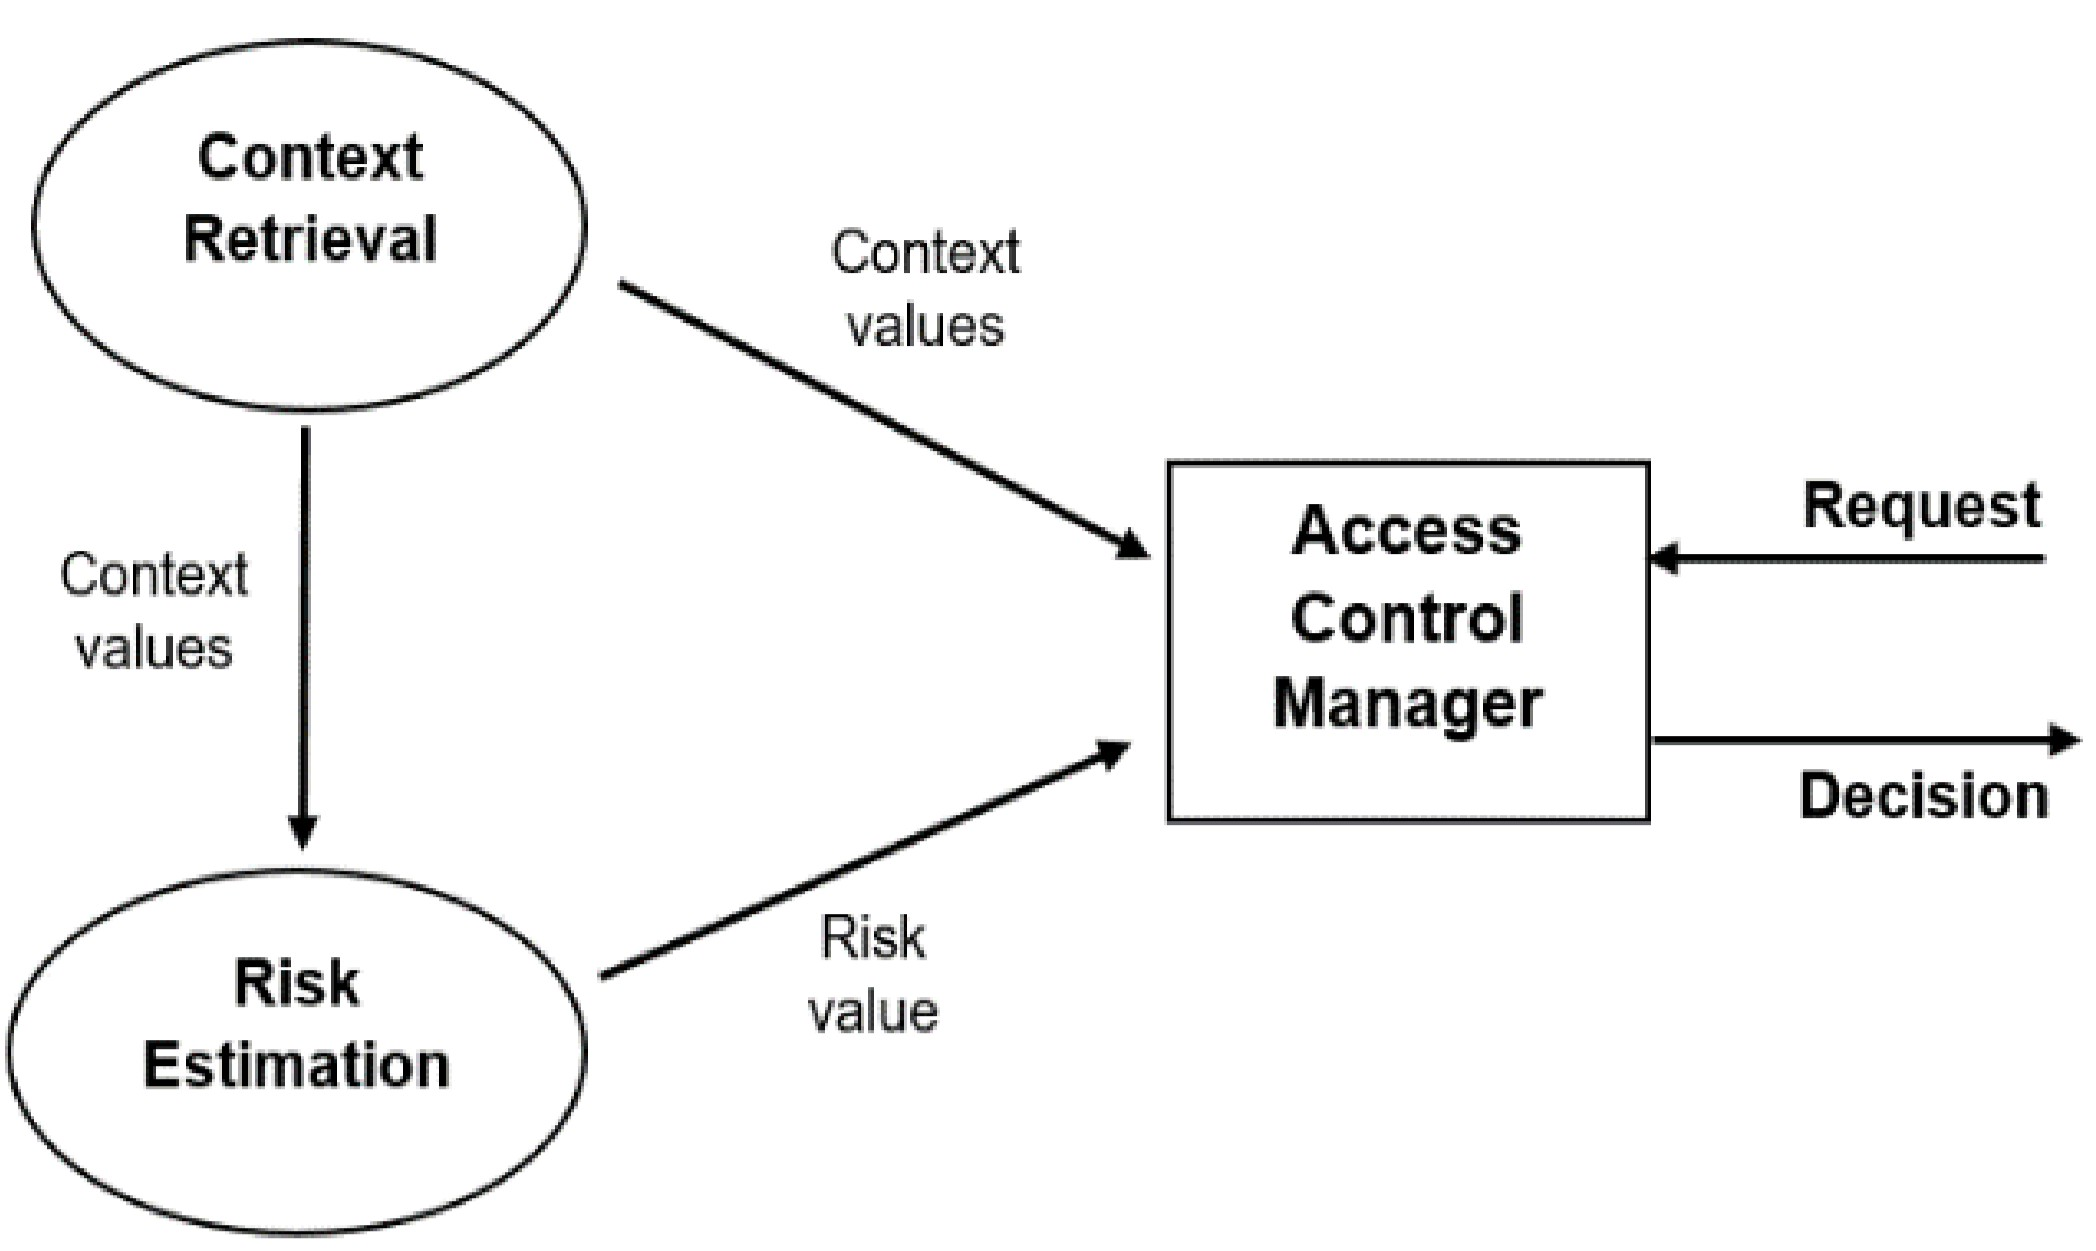
\includegraphics[width=.6\textwidth]{./figures/fig-rbac.jpg}
	\caption{基于风险访问控制概述~\cite{diep2007enforcing}}\label{fig:rbac}
\end{figure}

本章中,我们通过引入新的适应性风险量化方法和博弈论方法,扩展了基于风险访问控制基本模型。具体来说,风险估算过程与公式~\ref{eq:naive_risk}中的模型有所不同,并应用博弈论提出了一个新的组件。所提出的基于博弈论的风险自适应访问控制模型框架将在第~\ref{sec:framework}节中介绍。


\section{模型定义}
\label{sec:notations}


在由服务提供商~$\mathbf{S}$~(即系统)拥有的大规模用户~$\mathbf{U}$~(即访问主体)和隐私敏感资源(即访问客体~$\mathbf{O}$~)组成的系统中,所有用户都希望尽可能多地访问资源(甚至违反隐私权政策),且希望尽可能多地访问所有资源。但用户必须履行自己的职责,且不希望资源或服务提供商识别其恶意访问行为;资源(和/或服务提供商)希望尽早且尽可能多地识别恶意访问行为。因此,用户和服务提供商之间存在访问合作和隐私冲突。用户和资源都是自私的,因为其希望获得最大的利益,其将在每次访问中做出最佳策略选择以最大化自己的利益。对于特定用户~$u \in \mathbf{U}$~,其隐私侵犯行为与其他用户的隐私侵犯行为不同,因为其的职责彼此不同。但用户组~$g$~中总是有一些用户,这些用户在系统中具有相同或相似的职责(如所有胸外科医生在医院的HIS中必须履行类似的职责)。用户组~$g$~中的用户~$u$~的访问请求~$q_u$~想要访问某些资源~$~o_{u,q} \subset \mathbf{O}$~,~$~o_{g} \subset \mathbf{O}$~ 是组~$g$~的所有访问资源的资源集,若~$~o_{u,q}$~和~$~o_{g}$~之间的距离小于用户/访问主体~$s$~的阈值~$T_u$~,则访问请求~$q_u$~不侵犯隐私;否则,~$q_u$~侵犯了隐私。这意味着,若访问请求不服从具有类似职责的用户访问模式,则该请求会侵犯隐私。这种侵犯隐私的定义是合理的。因为同一组中的所有用户将以相似的方式执行其职责,因此服从这些职责的所有访问都将以相似的方式执行。 一旦访问不遵守工作职责,则模式将有所不同,且此访问侵犯了隐私。 在此,我们将~$~o_{u,q}$~与~$~o_{g}$~之间的距离~$D(o_{u,q},o_{g})$~定义为访问请求~$q$~的隐私风险~$r_q$~。
\begin{definition}[\textbf{隐私风险}]
	\label{def:privacy_risk}
	~$~o_{u,q}$~和~$~o_{g}$~之间的距离~$D(o_{u,q},o_{g})$~是隐私访问请求~$q$~的风险~$r_q$~ ,其中~$~o_{u,q}$~ 表示用户~$u \in g$~的访问请求q的目标资源集,~$~o_{g}$~表示用户组g的访问资源集。
\end{definition}

\begin{definition}[\textbf{隐私侵犯访问}]
	\label{def:privacy_violation_access}
	
	给定用户~$u$~的隐私阈值~$T_u$~和用户~$u$~的访问请求~$q$~。 若 ~$r_q > t_u$~,则~$q$~为\textit{隐私侵犯访问}; 否则,~$q$~是\textit{正常访问}。
\end{definition}



值得注意的是,可以根据不同用户的历史访问行为,将定义 ~\ref{def:privacy_violation_access}中的隐私阈值设置为不同的值。 特定用户的隐私阈值可以根据其历史访问行为(如使用贝叶斯方法或Markov方法)在不同时期内的变化来设置。

在访问活动过程中,在用户~$\mathbf{U}$~和访问客体~$\mathbf{O}$~之间存在博弈(实际上是由服务提供者~$\mathbf{S}$~而不是访问客体来博弈)。 在博弈中,参与者集~$\mathbf{A}=\{A_1,A_2,...,A_n\}$~由用户~$\mathbf{U}$~和服务提供商~$\mathbf{S}$~组成,每个参与者 ~$a_i$~都有一个策略集~$st_{A_i}$~,其中包含~$a_i$~的所有潜在动作。 对于一次访问过程中的所有参与者,都有一个效用函数~$u_{A_1,A_2,...,A_n}$~。 因此,~$~<\mathbf{A},\{St_{A_i}\},U_{A_1,A_2,...,A_n}>~$~是访问控制博弈模型。 在该模型中,策略和收益值与用户~$\mathbf{U}$~的访问隐私有关。

\section{理性RaBAC模型构建}
\label{sec:framework}


在本节中,我们利用博弈论提出了一个基于风险适应性访问控制模型的框架,并给出了该框架的详细工作流程。
\subsection{理性RaBAC框架}
\label{sec:hlframework}
\begin{figure}[htb]
	\centering
	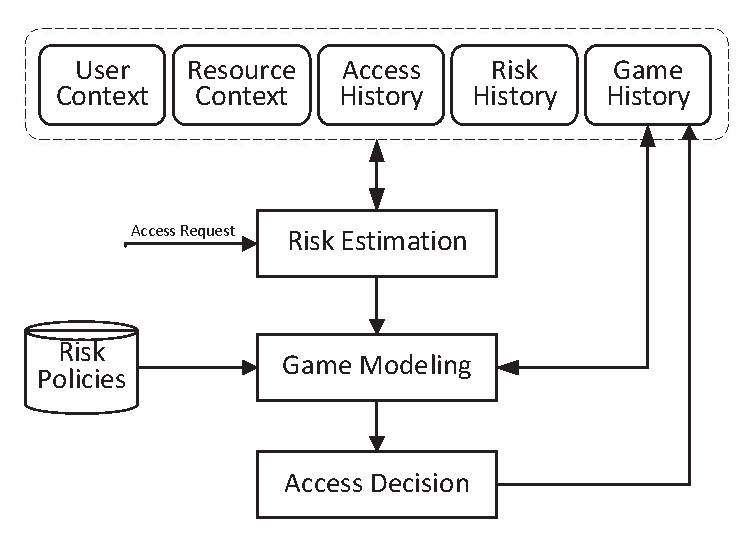
\includegraphics[width=.65\textwidth]{./figures/game-rbac-framework.eps}
	\caption{基于博弈论风险适应性访问控制框架 (RaBAC)}\label{fig:game-rbac-framework}
\end{figure}

基于博弈论的风险适应性的访问控制模型框架如图~\ref{fig:game-rbac-framework}所示。存储资源系统记录所有用户~$\mathbf{S}$~的用户上下文,所有资源~$\mathbf{O}$~的资源上下文,用户~$\mathbf{S}$~的访问历史记录,每个访问请求~$q$~的风险历史记录,以及博弈参与者~$\mathbf{A}$~中的博弈历史记录。收到访问请求~$q$~后,系统会通过使用用户上下文、资源上下文、访问历史记录和风险历史记录来自适应地计算~$q$~的隐私风险~$r_q$~,并更新风险历史记录(风险量化模块);然后,系统尝试通过识别~$q$~是否是违反隐私的行为来决定请求访问~$q$~的用户~$u$~的访问策略~$a_u$~,系统会根据用户的访问策略执行最佳策略~$a_u$~以获取最大利益,并更新博弈历史记录(计算博弈建模模块);系统采取的最佳策略是接收到的访问请求~$q$~的访问决策(访问决策模块)。如第~\ref{sec:notations}节中所述,可以定期更新“风险策略”模块中每个用户的风险阈值。
在此框架中,风险量化和博弈建模是核心模块,风险评估模块旨在实现对访问控制的适应性隐私风险计算,博弈建模模块旨在实现针对访问控制的最佳策略选择。


\subsection{理性RaBAC流程}


本节基于第~\ref{sec:hlframework}节中提出的框架,提出基于博弈的风险适应性访问控制模型的工作流程。

在XACML的标准框架中,有四个组件,策略执行组件(PEP),策略决策组件(PDP),策略访问组件(PAP)和策略信息组件(PIP)。 策略执行组件(PEP)收到用户的访问请求后,它将请求传递给策略决策组件(PDP),然后策略决策组件(PDP)向策略访问组件(PAP)和策略信息组件(PIP)请求其他信息,然后进行 决定接受还是拒绝该请求。 另外,策略执行点(PEP)难以处理与请求者的交互,策略访问组件(PAP)是静态的。 职责服务和策略信息组件(PIP)都缺乏风险管理。


在我们提出的访问控制框架中,对PEP,PIP和PAP进行了改进,并添加了新的三个组件,即博弈建模,策略风险评估组件(PREP)、会话控制和风险缓解服务组件。 然后,一旦PDP接收到来自经过身份验证的用户的访问请求,且在做出决定之前,它会请求与指定用户和历史记录相关的风险值,并构建一个博弈模型来做出访问控制决策。 此外,在由博弈建模组件执行决策后,一些反馈信息将提供给职责服务组件。 PREP可以实现对访问请求和用户的适应性隐私风险量化,博弈建模组件可以在用户(访问主体)和系统(访问客体)之间实现最佳访问策略选择。

\begin{figure}[htb]
	\centering
	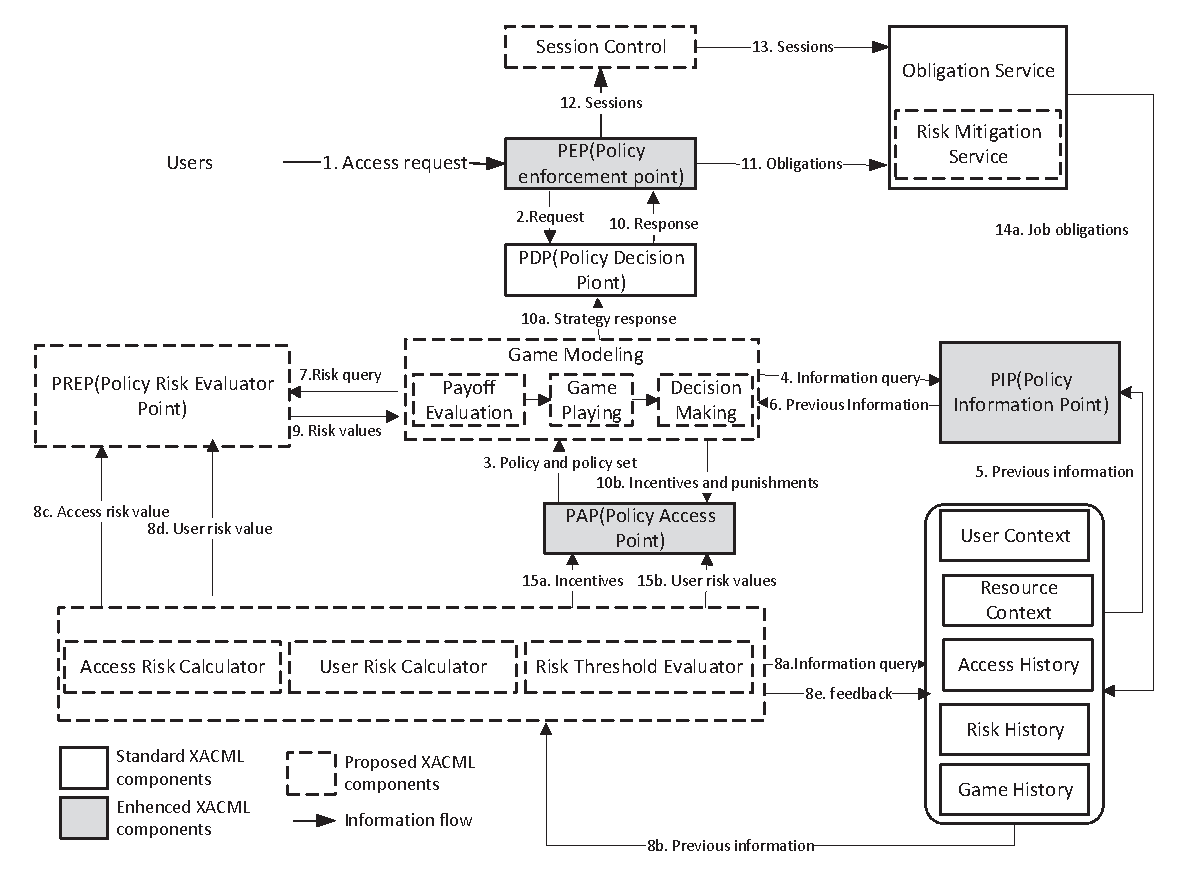
\includegraphics[width=1\textwidth]{./figures/game-rbac-workflow.eps}
	\caption{基于XACML的理性RaBAC的处理流程}\label{fig:game-rbac-workflow}
\end{figure}


所提出的理性RaBAC的过程流程如图~\ref{fig:game-rbac-workflow}所示,基于标准可扩展访问控制标记语言(XACML)提出了此框架,并展示了所提出的理性RaBAC的处理流程。该图中,所有新组件均以虚线突出显示,所有增强的组件均以浅灰色突出显示。工作流基于标准XACML,所有访问请求均由经过身份验证的用户发送。从步骤1到6,组件传递请求并收集先前的信息以进行访问控制;在查询了风险值之后(步骤7),策略风险评估组件(PREP)量化访问的隐私风险值和用户风险值(步骤8)。值得注意的是,PREP由访问风险计算组件,用户风险计算器和风险阈值评估组件组成。每个访问请求发出时,都动态计算一个访问请求隐私风险值和用户隐私风险值,且会根据当前用户的历史访问行为(如用户上下文、资源上下文、访问历史记录和风险历史记录)计算这两个值。若系统没有足够的历史记录,则PREP将根据推荐值来设置这两个值。与特定请求相关联的当前风险值返回到博弈建模(步骤9)。基于历史风险值和历史博弈行为,博弈建模为系统做出决策(如授权正常请求或拒绝正常请求)。将此决定转发给PEP,由其执行访问控制决策(步骤10)。无论是允许访问还是拒绝访问,PEP都会通知(步骤11)职责服务组件,该组件将决定是否需要风险缓解服务。在访问请求执行的延迟时间内,会话控制组件监视用户的行为,并管理访问会话(步骤12)。若在此会话中访问行为的风险过高,则会话控制会通知职责服务组件并控制此会话中的请求(步骤13)。职责服务将决定是奖励还是惩罚用户,并更新用户的特征(步骤14)。 PAP定期更新激励对策和用户风险值(步骤15)。

\section{隐私风险计算}
\label{sec:riskvalue}

风险值计算是基于风险访问控制的核心问题,设计一种适应性的风险计算方法十分重要,由此才能实现基于风险适应性的访问控制模型。 在本节中,为了能够实现适应性隐私保护需求,分别提出了针对访问请求和用户的适应性隐私风险量化方法。这些方法是由图~\ref{fig:game-rbac-workflow}中PREP组件的细节设计与实现。

\subsection{访问请求隐私风险计算}

除了第~\ref{sec:hlframework}中提出的框架之外,另一个主要问题是如何计算来自用户的每个访问请求的隐私风险。 对于来自用户~$u$~的特定访问请求~$q_u$~,可以通过按照定义~\ref{def:privacy_risk}来量化\emph{隐私风险} ~$r_{q_u}$~

存在一个用户组~$g$~使得~$u \in g$~,~$g$~中的所有用户都有相似的职责,且这些用户都遵守职责来访问相似的资源。假设在特定时间段~$T$~(例如24小时或1周),~$g$~的用户总共访问了基础系统~$n~$~次,且访问请求为~$q^g_{pre}=(q^g_1,q^g_2,...,q^g_n)$~,每个请求~$q^u_i$~旨在访问资源集~$r^g_i$~,其中~$1 \leq i \leq n~$~。
现在,~$q_u$~是~$u$~的当前访问请求,而~$r_u$~是预期访问的资源集。 因此,可以通过使用~$r_{q_u}$~的自信息和~$r^g_i$~的平均信息之间的距离来量化\emph{隐私风险} ~$r_{q_u}$~,如下
\begin{equation}\label{eq:privacy_risk_qu}
r_{q_u} = \dfrac{|Infor(R_{q_u})-\dfrac{\sum ^{n}_{i=1} Infor(R^g_i)}{n}|}{\dfrac{\sum ^{n}_{i=1} Infor(R^g_i)}{n}}, 
\end{equation}
其中~$infor(\cdot)$~表示资源集~$\cdot$~的信息量。 在一段时间内,组~$g$~中的所有用户访问资源都服从同一个概率分布,且可以通过每个访问请求中资源的访问频率来构造此分布。 因此,访问资源集~$r^g = \bigcup _{i=1}^n R^g_i=\{x_1, x_2, \cdots, x_m\}$~服从分布
\begin{equation}\label{eq:distribution_Rg}
\left(
\begin{array}{c}
X \\ P(X)
\end{array}
\right)
=\left(
\begin{array}{cccccccccc}
x_1 &  x_2 & \cdots & x_m
\\ p(x_1) &  p(x_2) & \cdots & p(x_m)
\end{array}
\right),
\end{equation}
其中~$p(x_j)=frequency(x_j)/\sum_{k=1}^m frequency(x_k)$~,而~$~frequency(x_j)$~表示~$R^g_1, R^g_2, \cdots, R^g_n~$~中~$X_j~$~的访问次数。因此, ~$R^g_i =\{x_1^{R^g_i},x_2^{R^g_i},\cdots, x_t^{R^g_i}\} \subset R^g$~,有
\begin{equation}\label{eq:information_Rgi}
Infor(R^g_i)=-\sum_{j=1}^t log(p(x_j^{R^g_i})).
\end{equation}

对于当前访问请求~$q_u$~的预期资源集~$R_{q_u}$~,可以将其分为两个子集, ~$R_{q_u}^* = R_{q_u}/R^g$~ 和 ~$R_{q_u}^{**} = R_{q_u} \cap R^g = \{x_1^{R_{q_u}^{**}},x_2^{R_{q_u}^{**}},\cdots, x_r^{R_{q_u}^{**}}\}$~,有

\begin{equation}\label{eq:information_Rqu}
\begin{split}
Infor(R_{q_u})&=Infor(R_{q_u}^{*})  +Infor(R_{q_u}^{**})
\\&=-\|R_{q_u}^*\|\cdot log(min(P(X)))-\sum_{j=1}^r log(p(x_j^{R_{q_u}^{**}})),
\end{split}
\end{equation}
其中,~$~||R_{q_u}^*||~$~表示~$R_{q_u}^*$~的阶。 在公式~\ref{eq:information_Rqu}中,若~$R_{q_u}^* \neq \emptyset$~,则~$R_{q_u}^*$~的任何元素都不属于~$R^g$~,且用~$R_g$~的最小访问集合代表它们。

在公式~\ref{eq:privacy_risk_qu}中,~$r_{q_u} \geq 0$~,且~$r_{q_u}$~越大,~$q_u$~的隐私风险就越高。我们可以在每个周期或每次访问中为用户~$u$~设置阈值~$r_{q_u}^{th}$~。 由定义~\ref{def:privacy_violation_access}知,若~$r_{q_u} > r_{q_u}^{th}$~,则~$q_u$~是违反隐私的访问;否则,~$q_u$~是正常访问,且可以根据~$u$~的历史访问行为在每个周期或每次访问中更新~$r_{q_u}^{th}$~。

\subsection{用户隐私风险计算}

每个周期开始时,都有一个由服务提供商给定用户~${u}$~的初始风险值~${r_u ^ 0}$~。 每次访问后,将根据该访问来更新用户~${u}$~的风险值。 假设用户~${u}$~第~${{i-1}}$~次访问后的风险值为~${r_u ^ {i-1}}$~,且~${q_u}$~是~${u}$~的当前访问请求,则~$~ {u}$~的该风险值将更新为~${r_u ^ {i}}$~。 若~${q_u}$~是隐私侵犯访问,则~${u}$~的风险值将增加,反之则降低,且该值快速增加而缓慢减小。 这在日常生活中是自然而然的事情,每个人都因为个人生活表现而存在特定的风险值,若他的表现不好,则风险会增加,而若表现良好,则风险会降低。 即使他做了一些新的好事,他周围的人也会保持警惕,风险值也不会迅速下降。但若他做了一些新的坏事,周围的人会更加警惕他,风险会迅速增加。 在这里,我们将用户的风险设置为
\begin{equation}\label{eq:userrisk}
r_u^{i}=\left\{ 
\begin{array}{cl}
r_u^{i-1}(1-\dfrac{\alpha}{r_{max}}), & \text{if } q_u \text{ is a normal access;}\\
r_u^{i-1}(1+\dfrac{\beta}{r_{max}})), & \text{otherwise.}
\end{array}
\right.
\end{equation}

在公式~\ref{eq:userrisk}中,~$\alpha~$~和~$\beta~$~是因子,~$r_{max}$~是最大的用户风险。

\section{基于扩展式博弈的理性RaBAC分析}
\label{sec:gamemodel}

\subsection{博弈模型构建}

博弈论是一种重要的数学工具,可用于相互冲突和合作的参与者间进行决策~\cite{owen2001game}。
在访问控制系统中,服务提供商(系统)和用户(或多个用户)对不同的利益感兴趣,且其必须彼此合作以实现自己的利益。在本章中,假设服务提供商(系统)和用户都是理性的,且将基于风险适应性的访问控制建模为一种隐私保护的博弈模型,其中涉及参与者、参与者策略和参与者效用函数。在这个博弈中,有两个参与者,服务提供者~$s$~和用户~$u$~。服务提供商拥有隐私敏感的资源(即访问客体),并希望授权正常访问请求并拒绝侵犯隐私的访问请求;用户是访问主体,其因为经济或其他利益而希望尽可能多地访问这些访问客体。用户~$u$~有两种策略,执行正常访问~$N$~和执行违反隐私的访问~$V$~;服务提供商有两种策略,分别授权正常请求~$G$~和拒绝正常请求~$D~$~。表~\ref{tab:payoff}展示了具有不同策略的参与者的效用函数。

\begin{table}[htb]
	\caption{支付矩阵}\label{tab:payoff}
	\centering 
	\begin{tabular}{cccc}
		\toprule
		\multicolumn{2}{c}{\multirow{2}{*}{}} & \multicolumn{2}{c}{User} \\
		\cline{3-4}
		& & ~$N~$~ & ~$V~$~ \\	
		\hline
		\multirow{2}{*}{Service Provider} & ~$G$~ &~$U_s^{G,N}$~, ~$U_u^{G,N}$~ & ~$U_s^{G,V}$~, ~$U_u^{G,V}$\\
		\cline{2-4}
		& ~$D~$~ & ~$U_s^{D,N}$~, ~$U_u^{D,N}$~ & ~$U_s^{D,V}$~, ~$U_u^{D,V}$\\
		\toprule
	\end{tabular}
\end{table}


因此,基于风险适应性的访问控制的博弈模型可以由元组~$~<s,u,A_s,A_u,U_{s,u}>~$~定义,其中~$s$~是服务提供者,~$u$~是用户,~$A_s=\{G,D\}$~是~$s$~的策略集,~$a_u=\{N,V\}$~是~$u$~的策略集,而~$u_{s,u}=\{U_s^{G,N}, U_s^{G,V}, U_s^{D,N}, U_s^{D,V}, U_u^{G,N}, U_u^{G,V}, U_u^{D,N}, U_u^{D,V}\}$~是具有不同策略的参与者的收益函数集。 该博弈是一个多次博弈,在每次迭代中,博弈者彼此了解并指导彼此的策略选择。同时,收益还取决于策略,历史访问和历史博弈策略。 因此,该博弈模型具有以下特征。
\begin{itemize}
	\item 两方博弈:在每次访问过程中,博弈者都是服务提供者和用户。
	\item 有限策略博弈:服务提供商和用户分别具有两个可选策略。
	\item 非零和合作博弈:若服务提供商和用户彼此合作,则均可获益。 如若用户执行常规访问且服务提供商准予访问,则它们将共同受益。
	\item 静态博弈:在每次访问之前,两个博弈者都不知道彼此的策略选择。
	\item 完美信息博弈:博弈者知道其在较早的访问过程中选择了哪些策略。
	\item 混合博弈:在此博弈中,用户出于不同的兴趣爱好而具有不同的类型,且服务提供商只是根据访问请求知道用户类型的分布。在不同的访问过程中,收益是不同的。
\end{itemize}

\subsection{博弈模型分析}

表~\ref{tab:payoff}中的效用函数表示如下,且我们分别分析了支付的组成部分。

\begin{itemize}
	\item ~$U_s^{G,N} >0$~是授权正常请求时服务提供商的效用。该效用是服务提供商通过授权常规正常请求而获得的收益,且该收益取决于当前访问请求~$q_u$~和用户的风险值~$r_u$~。有~$U_s^{G,N}= Sbenefit_g^n\times (r_{max}-r_u)$~​​,其中~$sbenefit_g^n~$~是服务提供商授权正常正常请求的基本收益,而~$(r_{max}-r_u)$~​​是因子。用户风险越低,服务提供商将获得更多的利益。
	\item ~$U_s^{G,V}<0$~是授权隐私侵犯访问请求时服务提供商的效用。此效用是由于授权当前隐私侵犯访问而导致的隐私损失,且受用户风险和访问风险的影响。有~$U_s^{G,V}= Sloss_g^v \times r_u \times r_{q_u}$~。
	\item ~$U_s^{D,N} < 0$~是拒绝正常访问请求时服务提供商的效用。该效用是拒绝正常访问请求所造成的效用损失,$U_s^{D,N}= Sloss_d^n \times (r_{max}-r_u)$。
	\item ~$U_s^{D,V} = 0$~是拒绝隐私侵犯访问时服务提供商的效用。
	\item ~$U_u^{G,N}$~是用户被授权其正常请求时的效用。此效用是正常访问带来的收益,并受用户风险值影响,有~$U_u^{G,N}= Ubenefit_g^n \times(r_{max} - r_u)$~。
	\item ~$U_u^{G,V} >0$~是用户被授权其隐私侵犯访问请求时的效用。该效用包括几个部分,正常利益和通过授权当前访问请求而带来的额外利益,并受用户和访问请求的当前风险的影响,有~$U_u^{G,V}= Ubenefit_g^n\times(r_{max} - r_u) + Uextra_g^v \times r_u\times r_{q_u}$~
	\item ~$U_u^{D,N} =0$~是用户被拒绝其正常访问时的效用。
	\item ~$U_u^{D,V}<0$~是用户被拒绝其隐私侵犯访问请求时的效用。该效用是服务提供商对用户的一种惩罚,并受到用户和访问风险的影响,有~$U_u^{D,V}= Upunish \times r_u \times r_{q_u}$~。
\end{itemize}

在此多次博弈中,可以分别考虑每次博弈的策略选择关系,并将每个子博弈视为一个独立博弈。假设此博弈中有~$T$~次子博弈,且~$\sigma_1^*, \sigma_2^*, \cdots, \sigma_T^*$~是独立阶段博弈的Nash均衡策略的有序序列,然后该序列存在子博弈完美均衡,且均衡路径由~$\sigma_1^*, \sigma_2^*, \cdots, \sigma_T^*$~生成。在每个阶段的博弈中都会求得最佳策略选择解。假设博弈中服务提供者的混合策略是~$(p,1-p)$~,其中服务提供者以概率~$p$~授权访问请求,并以概率~$1-p$~拒绝访问请求;用户的混合策略是~$(q,1-q)$~,其中{~$q$~}是用户选取正常访问的概率,而~$1-q$~是用户选取隐私侵犯访问的概率。因此,用户的预期效用为
\begin{equation}
\begin{split}
U_u&= (1-q)(p\times U_u^{G,N}+ (1-p)\times U_u^{D,N})+ q(p\times U_u^{G,V}+(1-p)\times U_u^{D,V})\\
&=(1-q)\times p \times Ubenefit_g^n \times(r_{max} - r_u)+ q[p(Ubenefit_g^n\times(r_{max} - r_u) \\
&+ Uextra_g^v r_ur_{q_u})+(1-p)Upunishr_ur_{q_u}].
\end{split}
\end{equation}

通过求解微分方程~$\frac{\partial U_n}{\partial q}=0$~,得到~$(p^*,1-p^*)$~,其中
\begin{equation}
p^*=\dfrac{Upunish}{Upunish-Uextra_g^v}.
\end{equation}

因此,~$(p^*,1-p^*)$~是服务提供商混合策略的Nash均衡。在这种情况下,服务提供商希望惩罚并减少隐私侵犯访问。同样,可以为用户求得混合策略~$(q^*,1-q^*)$~的Nash均衡,其中
\begin{equation}
q^*=\dfrac{Sloss_g^v r_u r_{q_u}}{Sloss_g^v r_u  r_{q_u} +(Sloss_d^n -Sbenefit_g^n)(r_{max}-r_u)}.
\end{equation}

在这种情况下,服务提供商和用户都可以获得最大的收益,且单次子博弈都可以达到Nash均衡。因此,用户将执行正常访问,而服务提供商将准许用户的正常访问请求。 因此,服务提供商通过限制隐私侵害访问来保护信息资源中涉及的隐私信息。

\section{比较与分析}
\label{sec:comparison}

尽管有文献~\cite{ni2010risk,wang2011quantified,shaikh2012dynamic,santos2016framework,wang2019game,zhang2015towards,zhen2015risk,zhang2018privacy,gao2018game,liu2016dynamic,helil2017non,hu2014game}和本文第~\ref{chap:RaBAC-for-privacy}章研究了与风险或博弈论相关的不同访问控制模型,但本章的工作与这些研究相比明显优势,如表~\ref{tab:comparison}所示。

\begin{table}[htb]
	
	\caption{本章所提出模型与已有工作的对比}\label{tab:comparison}
	\small
	\centering 
	\begin{tabular}{ccccc}
		\toprule
		文献 & 访问控制目的 & 风险量化方法 & 博弈参与者 & 博弈模型 \\
		\hline
		Ni等~\cite{ni2010risk} & 安全防护 &静态安全风险&-&-\\ 
		Shaikh等~\cite{shaikh2012dynamic} & 安全防护 & 动态风险与信任&-&-\\
		dos Santos等~\cite{santos2016framework} &云安全防护 & 多因子聚合风险 &-&-\\
		本文第\ref{chap:RaBAC-for-privacy}章& 云数据隐私保护& 基于熵和Markov的动态风险 & - & -\\
		Wang和Jin~\cite{wang2011quantified} & 医疗信息隐私保护 & 静态隐私风险 &-&-\\
		Zhen等~\cite{zhen2015risk} & 医疗信息隐私保护& 基于熵的动态风险 & - & -\\
		Zhang等~\cite{zhang2018privacy} & 医疗信息隐私保护& 基于条件概率和Markov的动态风险 &-&-\\
		Liu等~\cite{liu2016dynamic} & 蜂窝网络接入安全&-&	多参与者&	序贯博弈\\
		Gao等~\cite{gao2018game} & 云数据安全防护& -&两方参与者&重复博弈\\
		Zhang等~\cite{zhang2015towards} & 安全防护& 信任 & 两方参与者& 非零和多次博弈\\
		Wang等~\cite{wang2019game} & 安全防护& 动态信任 & 两方参与者 & 非零和多次博弈\\
		Hu等~\cite{hu2014game} & 社交网络隐私保护&静态隐私风险&多方参与者&	多控制博弈\\
		Helil等~\cite{helil2017non} & 通用访问控制场景&动态安全风险&两方参与者&非零和合作博弈\\
		本章工作 & 数据隐私保护& 基于自信息和Markov动态隐私风险 & 两方参与者& 非零和多次博弈\\
		\bottomrule 
	\end{tabular}
\end{table}


在表~\ref{tab:comparison}中,文献~\cite{ni2010risk,shaikh2012dynamic,santos2016framework,wang2011quantified,zhang2018privacy,zhen2015risk}和本文第\ref{chap:RaBAC-for-privacy}章都设计了非混合风险的访问控制。Niel等~\cite{ni2010risk}和Shaikh等~\cite{shaikh2012dynamic}的目标是分别通过量化静态安全风险和动态风险来保护系统的安全。 dos Santos等~\cite{santos2016framework}提出了基于风险自适应的访问控制模型,以通过不同的动态风险估算方法保护云安全。本章的模型是面向以数据为中心的系统中数据隐私保护而非安全保护,同时适用于本地化和云系统。尽管文献~\cite{wang2011quantified,zhen2015risk,zhang2018privacy}提出了不同的用于保护隐私的基于风险访问控制模型,但这些模型仅适用于医疗保健系统,且可以保护病历的隐私,这些工作改进了风险量化的方法。本章模型不仅可以应用于医疗保健系统,还可以应用于其他方案(如机密信息系统或以数据为中心的系统)。此外,本章通过Shannon信息量和Markov设计了包括访问请求和用户的动态隐私风险值,而非通过熵~\cite{zhen2015risk}、条件概率~\cite{zhang2018privacy}的静态隐私风险~\cite{wang2011quantified}。此外,所有这些工作都是基于非博弈论的方法,本章的工作是基于博弈论的基于风险适应性访问控制模型。在所提出的访问控制模型中,所有参与者都是理性自私的,其在每次访问迭代中都做出了最佳策略选择。


有一些研究是基于博弈论的访问控制模型~\cite{liu2016dynamic,gao2018game,zhang2015towards,wang2019game,hu2014game,helil2017non}。 但只有Hu等~\cite{hu2014game}和Helil等~\cite{helil2017non}的工作是基于风险访问控制模型,而Liu等~\cite{liu2016dynamic}和Gao等~\cite{gao2018game}只是利用博弈论扩展了传统的访问控制,并应用于蜂窝网络接入和云数据访问 控制方面,Zhang等~\cite{zhang2015towards}和Wang等~\cite{wang2019game}专注于通过信任而不是风险进行安全保护。 尽管Zhang等~\cite{zhang2015towards}、Wang等~\cite{wang2019game}的模型和本章都是都是两人非零和多阶段博弈,但应用场景和量化方法也有所不同,本章的模型适用于数据隐私保护,并基于一种可调整的隐私风险量化方法。 除此之外,这些工作~\cite{liu2016dynamic,gao2018game,zhang2015towards,wang2019game}都不是基于风险访问控制,而本章的模型是基于风险适应性的访问控制。

与本章最相近的研究,如文献~\cite{hu2014game}和~\cite{helil2017non}是基于风险和博弈论的访问控制模型,但这些研究与本章不同。 Hu等~\cite{hu2014game}提出了一种用于社交网络中通过静态隐私风险量化保护隐私的多方控制博弈。
本章工作不是针对社交网络,且博弈模型与Hu等~\cite{hu2014game}不同,Hu等~\cite{hu2014game}根据用户关系设计了静态隐私风险,而我们模型中的隐私风险则根据用户的历史访问请求而动态自适应更新。在文献~\cite{helil2017non}中,作者针对一般访问控制模型提出了基于风险信任的访问控制的两人非零和合作博弈分析。该研究不是为了保护隐私,且该模型的访问风险是基于历史访问信息信任值进行量化。但是本章的研究是为了在开放、以数据为中心的系统中保护隐私,并根据直接量化访问请求和用户的隐私风险。此外,我们还为访问控制模型提出了一个基于XACML的框架和详细的工作流程。

\section{小结}\label{sec:conclusions}

在本章中,为了保护访问控制系统中数据隐私的目的,提出了一种基于风险适应性的访问控制模型,并将此访问控制建模为一个多次的二人博弈。 在该模型中,引入了一些新的组件,如风险评估和博弈建模,并通过使用Shannon信息来量化访问风险和用户风险。 最后,我们为每次访问迭代求得了子博弈精炼Nash均衡,服务提供商和用户都希望在这种状态下表现良好,且通过限制侵犯隐私的访问请求来保护数据隐私敏感。 比较表明,此访问控制模型比以前的工作具备更多优势,且实现了良好的隐私保护性能。%结论
\chapter{基于演化博弈的理性隐私风险访问控制模型}
\label{chap:evolutionary-rabac}

\textit{ }

\textit{以数据为中心的大规模用户系统中,现有基于理性的访问控制模型难以满足适应性保护隐私的需求,且博弈参与者的完全理性假设太强,不符合实际场景。针对此问题,本章提出一种面向隐私保护的多参与者理性风险自适应访问控制模型,包含了新的隐私风险量化模块和演化博弈决策模块。首先,基于Shannon信息对访问请求的数据集隐私信息量进行量化,构造了访问请求隐私风险函数和用户隐私风险函数;其次,基于演化博弈在有限理性假设下构建多参与者的访问控制演化博弈模型,利用复制动态方程分析了访问控制参与者的动态策略选择和演化稳定状态形成机理,提出了隐私风险访问控制博弈演化稳定策略的选取方法。仿真实验和对比表明,所提出的访问控制模型能够有效动态自适应地保护敏感信息资源系统中的隐私信息,具有更好的隐私风险适应性,有限理性参与者的动态演化访问策略选取更加符合实际场景。}

\section{概述}
访问控制是信息系统保障数据安全和系统安全的重要基础性工具~\cite{sandhu1994access}。云计算、大数据及物联网的兴起和发展,使得网络和系统更加复杂、开放,数据安全和隐私需求更加多样化,用户和系统的角色、属性更加难以发掘,需要更加动态化、自适应、细粒度的访问控制模型以满足新环境下的安全和隐私需求~\cite{li2017access}。

强制访问控制~\cite{mccune2006shamon}、自主访问控制~\cite{downs1985issues}、基于角色访问控制~\cite{sandhu1996role}等访问控制模型的访问策略是静态的、访问控制粒度粗放,且面对大规模用户的开放系统,难以预先指定用户身份,故这些模型难以适用云计算、大数据和物联网中的新型应用场景。基于属性访问控制~\cite{wang2010hierarchical}因其访问控制粒度较细、不需要指定用户身份或角色而受到广泛的关注,在云计算场景、物联网等得到了应用,但其需要预先定义访问策略,属性挖掘与属性撤销的计算和实施都比较困难,不能适应动态访问控制需求~\cite{servos2017current}。为了解决基于属性访问控制等传统访问控制模型存在的诸多问题,风险和信任被先后引入到访问控制中,提出了基于角色或属性的风险访问控制模型~\cite{dimmock2004using,kandala2011attribute,krautsevich2014towards},一定程度上解决了用户访问的动态控制,并进一步发展为基于风险访问控制~\cite{cheng2007fuzzy,ni2010risk},更加适用于大数据环境的访问控制需求。医疗、社交网络和位置信息服务等系统的大量多样性数据集访问有了开放性、动态性和隐私敏感需求,隐私侵犯来自内部和外部访问~\cite{boulares2017insider},迫切需要能对用户隐私信息在访问过程中进行隐私保护。

访问控制模型中存在授权不足或过度授权的现象,引发数据和系统安全、隐私泄露的风险,亟需能够平衡安全隐私与授权度间的解决方案。访问控制可看做访问主体(用户)与访问客体(服务提供者或系统)间的冲突与合作。博弈论~\cite{owen2001game}作为一种解决参与者对抗与合作,并使得参与者获取最大化利益的数学工具,被自然引入到访问控制以平衡安全和访问效用~\cite{helil2017non,gao2018game,wang2019game},但现有研究多集中于二人访问控制博弈,要求参与者是完全理性的,难以客观描述访问控制模型中多个用户与系统间的博弈。

本章针对现有访问控制模型难以满足适应性保护隐私的需求,且其访问控制博弈模型难以刻画多用户与系统间的非完全理性对抗与合作问题,基于用户访问隐私风险量化和多人演化博弈,面向开放环境的数据存储隐私保护,提出一种基于演化博弈的多参与者的理性风险访问控制模型,并分析其演化稳定状态和演化稳定策略求解。该访问控制模型在保持风险访问控制优势的同时,通过用户访问隐私风险约束,限制用户高隐私风险的恶意、好奇访问请求,实现隐私保护,同时仅假设参与者有限理性,用多人非合作博弈对多用户对系统资源访问的策略、收益进行分析,通过演化达到博弈演化稳定状态实现了用户和系统间的均衡及稳定,有效平衡隐私保护和访问效用,更加符合现实场景中用户与系统间的策略动态变化选取特征。具体而言,本章的贡献如下:
\begin{enumerate}
	\item 面向开放环境的数据共享隐私保护,在有限理性假设下,通过分析多用户场景的敏感数据隐私保护访问控制问题及需求,提出了一种包含隐私风险量化和演化博弈模块的多人隐私风险自适应访问控制模型。减弱了现有理性访问控制模型的参与者完全理性假设,将二人博弈扩展为多人的群体博弈,且能够适应以数据为中心的系统敏感数据隐私保护需求。
	\item 在“Need-to-Know”的原则下,根据用户访问请求敏感资源的特征,定义了基于信息量化的访问请求隐私风险和用户隐私风险,并给出了自适应的动态隐私风险计算方法。
	\item 对所提出的多用户隐私保护访问控制模型构建了演化博弈模型,提出了基于隐私风险自适应的效用函数,并利用动态复制方程分析并求解了所提出的访问控制模型的博弈演化均衡策略。
	\item 利用动力学理论对所提出的访问控制模型的演化博弈过程进行了仿真,结果表明所提出的多用户隐私风险自适应访问控制模型可在有限理性的演化博弈过程中达到演化稳定状态,能够实现自适应风险的敏感数据隐私保护。
	\item 与相关基于风险访问控制模型和理性访问控制模型相比,所提出的访问控制模型在以数据为中心的信息系统隐私保护方面具有更好的优势,风险自适应程度好、访问控制参与者假设更符合实际、能达到较好的隐私保护效果。
\end{enumerate}



\section{相关工作}

在风险访问控制~\cite{mcgraw2009risk}的概念提出后,Cheng等~\cite{cheng2007fuzzy}用多层安全的思路量化了风险,将风险划分为不同等级,实现了该模型的一个实例,但该量化方法缺乏数学理论支持;随后,Ni等~\cite{ni2010risk}用模糊推测理论在Cheng等的基础上重新量化风险,使得风险量化满足合取、析取及取反操作需求,用以处置访问控制中的紧急访问需求。但文献~\cite{cheng2007fuzzy,ni2010risk}中风险量化是静态的,因无法应对访问需求多样、无法预先定义安全等级而缺乏适用性,同时不能满足系统的隐私保护需求,也不能对访问主体的高风险访问进行激励约束。

针对文献~\cite{cheng2007fuzzy,ni2010risk}的风险量化静态、不适应高敏感环境问题,Shaikh等~\cite{shaikh2012dynamic}利用历史访问行为进行风险和信任动态量化,其风险通过威胁概率和数据泄露影响量化,利用指数移动加权平均算法提出了动态风险的访问控制,以保护系统安全。Armando等~\cite{armando2015balancing}参照基于策略访问控制,将访问风险和用户信任进行对比,通过增强用户信任、削减访问安全风险以平衡二者,保护系统资源安全。Diaz-Lopez等~\cite{diaz-lopez2016dynamic}将访问风险量化多层分类,并定义对应的风险控制策略,利用遗传算法为动态访问的访问行为提供安全应对措施,以保护高敏感环境的数据安全。但这些方法在风险量化过程中所依赖的信息过多,在实际环境中不能全部获取,易使风险量化不精确而导致访问控制失败。为此,dos Santos等~\cite{santos2016framework}提出基于权重的多因子聚合风险量化,并提出一种面向云安全的风险访问控制框架。但文献~\cite{shaikh2012dynamic,armando2015balancing,diaz-lopez2016dynamic,santos2016framework}所提出的方法因风险量化是面向安全的,不适用于隐私保护需求。

为了隐私保护需求,Wang等~\cite{wang2011quantified}针对医疗信息系统,利用信息熵按照“Need-to-know”的原则,通过对恶意医生和诚实医生间访问信息的不同,对医生访问病患信息的风险进行量化,提出了一种灵活的风险访问控制模型,但该模型预先假定了诚实医生的行为,风险量化缺乏适应性以对应访问需求变化。在文献~\cite{wang2011quantified}的基础上,惠榛等~\cite{hui2015risk}利用EM二分算法对基于信息熵的医生访问行为进行区分,监测和控制隐私侵犯的高风险访问性。Zhang等~\cite{zhang2018privacy}定义了隐蔽非诚实医生行为,基于时间盒和迭代实现了以主题建模为核心的风险自适应访问控制模型。文献~\cite{wang2011quantified,hui2015risk,zhang2018privacy}所提出的方法仅适用于医疗信息系统隐私保护,且并未考虑访问主体与客体间的合作与对抗。针对用户匿名保护需求,Armando等~\cite{armando2015risk}将风险访问控制与匿名访问结合,同时考量匿名与数据效用,在匿名系统中抑制高风险访问。本文第\ref{chap:RaBAC-for-privacy}章利用Markov模型对主体访问行为的风险进行量化,并提出了基于信用卡额度约束的风险访问控制模型,在云环境数据隐私保护中激励低风险访问行为,约束高风险访问行为。

与传统访问控制模型中的参与者博弈~\cite{gao2018game,hu2014game,liu2016dynamic}类似,基于风险访问控制中的访问主体与客体间也存在二人或多人冲突与合作关系。Helil等~\cite{helil2017non}基于二人非合作博弈模型,利用用户信任和访问风险刻画效用函数,分析了风险访问控制模型中的子博弈完美Nash均衡,有效的保证了访问控制决策的科学性,其并未考虑多访问主体访问客体间的冲突与合作。

本章针对开放、动态的大规模多样性数据访问隐私保护需求及多用户与系统间的冲突与合作关系,提出一种多参与者的理性隐私风险自适应访问控制模型。相比于已有工作,该模型仅要求参与者有限理性,通过对访问控制过程中的多参与者的行为、策略和隐私效用的博弈要素进行多参与者演化博弈建模,解决了现有文献对风险访问控制参与者行为刻画不足的问题;通过对历史访问行为和资源建模,利用信息论对访问请求和用户的隐私侵犯风险量进行评估,仅用少量先验信息资源,减少了对系统历史访问信息的要求;仅利用隐私风险量化,不再依赖信任机制,简化了模型的设计复杂度;通过多人演化博弈的演化稳定策略状态求解,不但有效约束了高隐私风险的访问请求,激励用户进行低隐私侵犯访问,且实现了动态风险访问控制的优化访问决策,可有效保护系统隐私数据。

\section{基于演化博弈的有限理性RaBAC模型构建}
本节首先分析本章所构建的多参与者博弈的风险访问控制模型所要解决的问题,其次提出多参与者隐私风险访问控制模型。

\subsection{有限理性RaBAC模型问题描述}
\label{subsec:issues}
在医疗信息系统、情报信息系统、外包计算数据池等环境中存在大量包含个人隐私信息数据,访问的用户量大,且用户不断动态更新访问需求,用户的角色、属性、访问策略等信息难以预先定义,用户为完成其职责不断动态变化访问请求,这些信息难以随用户的访问而动态更新。为了保护隐私信息,需对访问请求的数据所包含的隐私量进行量化,现有的风险访问控制模型难以对隐私进行有效描述和精确动态的量化。访问控制模型中,参与者间是长期的多次访问控制交互,在访问过程中往往无法对所有背景知识和他人的信息全部了解,也无法在每次访问时理性地做出最佳的策略选择,但参与者可模仿其他参与者的高收益策略,调整其后续行为策略,但对非完全理性的多参与者间的冲突与合作博弈行为进行描述极为困难,如何设计激励相容的机制使得参与者诚实合作,尽可能不侵犯隐私,且取得高收益,并使参与者短期利益和长期利益一致。非理性参与者的多人扩展式动态博弈是一个复杂的博弈模型,均衡的存在性证明和求解都极为困难,通过多次交互式博弈和参与者自发策略调整可使博弈逐步处于一种相对稳定状态,即用户稳定地请求低隐私风险访问,即使偶有高隐私风险访问,也会后续调整为低隐私风险访问策略,系统稳定地授权用户低隐私风险访问,即使偶有拒绝授权此类访问,也会后续调整授权策略。
在所提出面向隐私保护的多参与者理性风险访问控制模型中,试图通过以下措施解决上述问题。
\begin{enumerate}
	\item 定义并量化访问请求的隐私风险。依据“Need to Know”的原则,用户为完成工作职责而访问到信息资源中的敏感信息不应当是隐私侵犯,除此之外的访问应当认为是隐私侵犯。在经认证的用户群体中,用户会优先完成自己的职责,其大多数访问请求都是为了完成自己的职责,则该用户单次访问请求与其历史访问请求产生偏移距离,偏离的越远,其违背“Need to Know”原则越严重,访问的隐私信息资源的隐私量越大,隐私风险越高。
	\item 定义并量化用户的隐私风险。将具有相似访问请求行为模式的用户群看作具有相同职责的用户,在历史访问过程中,某一用户的访问偏离该用户群的距离越远,其违背“Need to Know”原则越严重,其用户隐私风险越高;此外,其用户隐私风险直接受其历史访问行为影响,单次的高隐私风险访问将使用户隐私风险提高很快,而单次的低风险访问对用户隐私风险的降低影响较小
	\item 构建演化博弈以刻画多用户和系统的非理性多次博弈。不再对参与者进行绝对理性的假设,而将所有用户和系统视为有限理性的参与者。将访问控制系统的所有参与者看作用户群体和信息资源系统群体,两个群体之间进行多次动态的博弈。博弈过程中,群体中的低收益者会模仿高收益参与者的博弈选择策略,不断进行演化,最终达到稳定的状态,该状态下的参与者策略选择即为演化稳定策略,是参与者的最优策略。
	\item 对(3)中博弈模型设计激励相容的机制。在博弈模型中,对用户的激励主要是通过效用函数的设计来实现。本章对用户的效用函数设计,通过隐私风险量化来计算访问请求的隐私风险和用户隐私风险,分别兼顾短期利益和长期利益。效用函数受到这两个变量的影响,使得对用户而言,长期诚实地访问能使其获得更高的收益,短期的恶意访问虽然能有额外的获得,但却远低于长期收益。同时通过惩罚机制,对短期恶意访问的隐私侵犯行为进行惩罚。促使用户能长期诚实地访问系统。同时,在尽可能吸引更多用户访问系统的前提下,亦可阻止恶意的隐私侵犯访问请求,使薪资资源系统能够更加精确、动态地做出有效的策略选择,授权诚实的正常访问,拒绝侵犯隐私的恶意访问。
	\item 对(3)中的博弈模型求解。利用动态复制方程在动力学原理下,分析所提出风险自适应访问控制演化博弈模型的参与者收益函数和信念函数,进一步分析其演化稳定状态及其机理,提出演化稳定策略的求解公式。在不同的初始状态下,通过博弈的不断演化,访问控制博弈总能达到某个演化稳定状态,该状态下的博弈策略选择即为参与者的最优策略。
\end{enumerate}

\subsection{基于演化博弈的理性RaBAC模型}
面向隐私保护需求,多用户和信息资源系统间的有限理性参与者隐私风险访问控制模型如图~\ref{fig:Evolutionary-game-Rabac}所示,包含访问请求决策管理模块、演化博弈建模模块、隐私风险评估模块、上下文信息模块和风险策略模块。

\begin{figure}[htbp]
	\centering
	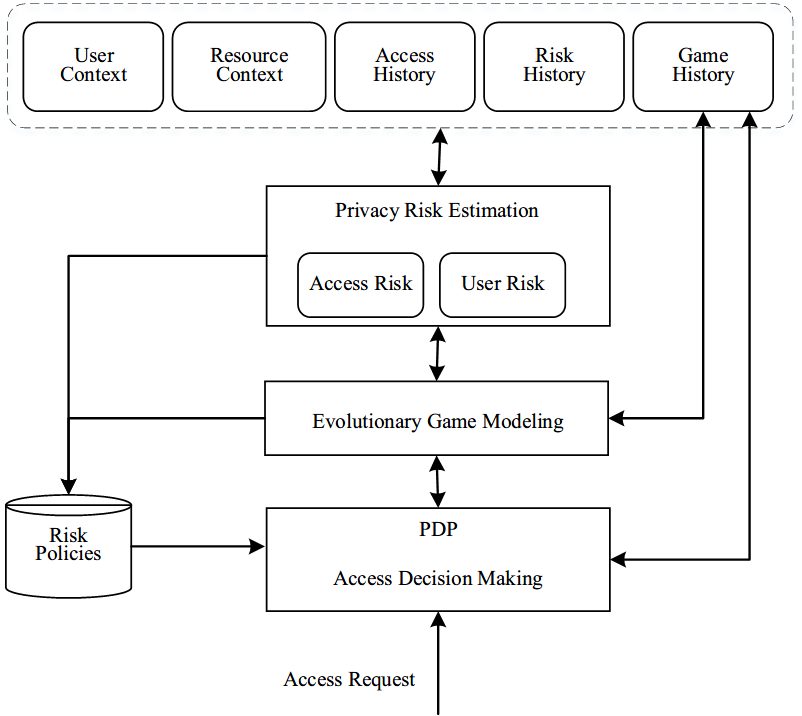
\includegraphics[width = 0.6\linewidth]{./figures/Evolutionary-game-Rabac.png}
	\caption{基于演化博弈的隐私风险访问控制模型}
	\label{fig:Evolutionary-game-Rabac}
\end{figure}

图~\ref{fig:Evolutionary-game-Rabac}中,访问请求决策管理模块接收用户访问请求,根据博弈结果和风险策略模块提供的信息做出授权或不授权等访问决策,并反馈至上下文信息模块;演化博弈建模模块对参与访问控制的用户和系统进行博弈演化,博弈过程中通过隐私风险信息和上下文信息进行动态策略选择,并给出演化策略结果,并将结果反馈给上下文信息模块和访问请求决策管理模块;隐私风险量化模块对访问请求隐私风险和用户隐私风险进行动态量化,支撑演化博弈建模和风险策略更新,并将结果反馈存储至上下文信息模块中;上下文信息模块动态记录并存储用户、信息资源、访问历史、历史隐私风险值、历史博弈策略及收益函数等信息;风险策略池动态更新各用户的隐私风险访问控制策略。

\section{隐私风险定义及自适应计算方法}
本节针对第~\ref{subsec:issues}节所述隐私风险量化问题,分别定义访问请求隐私风险和用户隐私风险,并给出自适应风险计算方法。
\subsection{访问请求隐私风险}

访问控制系统中,信息资源可以通过自然语言处理或机器学习的方式进行标注化,使得所有信息资源记录或原子集合都包含和系统资源使用功能、目的相关的标签信息,如医疗系统中所有的医疗数据可以根据ICD-10标准进行标签化处理,情报系统中所有的情报信息可按照情报属性和功能进行标签化标注。将访问控制过程按照时间划分为不同的时间段~${{T}_{0}},{{T}_{1}},{{T}_{2}},\cdots ~$~,每个时间段是一小时、一天或一周等。用户U在前一个时间段T内和当前时间向系统发出了~$n$~次访问请求~$q_{1}^{U},q_{2}^{U},\cdots ,q_{n}^{U}$~,对应的访问信息资源集合(实际应用中利用信息资源集合对应的标签集合进行风险计算)为~$R_{1}^{U},R_{2}^{U},~$~ ~$\cdots ,R_{n}^{U}$~,则U访问的信息资源集合为~$R_{{}}^{U}\text{=}\bigcup\nolimits_{i=1}^{n}{R_{i}^{U}}$~。当前用户~$U$~的访问请求为~$q_{0}^{U}$~,该请求对应的系统信息资源集合为~$R_{0}^{U}$~。根据各用户的历史访问信息资源集合的相似性和聚类,可将具有相似访问行为的用户划分为一组,在某一组中,所有的用户具有相同的系统职责,在访问行为上仅有较小的差异。设用户~$U$~属于用户分类组~$g$~,用户分类组~$g$~在前一个时间段T内和当前时间段内,访问的信息资源集合为~$R_{{}}^{g}$~。则用户~$U$~的当前访问请求~$q_{0}^{U}$~隐私风险为

\begin{equation}
r(q_{0}^{U})=\begin{cases}
1, & \text{ 若 } R_{0}^{U}/{{R}^{g}}\ne \varnothing \\ 
\alpha \frac{-|R_{0}^{U}/{R}^{U}|max_{x\in R_{0}^{U}/{R}^{U}}logp(x)}{-\sum_{x\in{R^U}}logp(x)}+ \beta \frac{-\sum_{x\in R_0^U \cap  R^U}logp(x)}{-\sum_{x\in  R^U}logp(x)}& \text{若 } R_{0}^{U}/{{R}^{g}}=\varnothing 
\end{cases}
\end{equation}
其中~$p(x)$~表示~$x$~在~$R_{{}}^{g}$~中的概率,~$1>\alpha >\beta >0$~,且~$\alpha \text{+}\beta \text{=}1$~。
根据用户组~$g$~中用户的访问请求风险值的历史及分布可利用分位数设置阈值~${{t}_{g}}$~,若~$r(q_{0}^{U})>{{t}_{g}}$~,则定义~$q_{0}^{U}$~为隐私侵犯访问请求,否则其为非隐私侵犯访问请求。特别注意的是,前述定义是从系统的角度看待某一访问请求,用户~$U$~会主动选择正常访问或隐私侵犯访问,但系统仅根据访问请求本身来判定,可能将用户的正常访问识别为隐私侵犯访问,亦有可能将用户的隐私侵犯访问识别为非隐私侵犯访问。当将某一访问请求识别为隐私侵犯访问时,用户可通过风险消除措施降低隐私风险,文献~\cite{diaz-lopez2016dynamic}讨论了相关措施。

\subsection{用户隐私风险}
用户~$U$~的隐私风险是根据其访问行为特征而发生变化,当用户访问请求隐私风险值高,则用户的隐私风险提高;用户的访问请求隐私风险值低,则用户隐私风险降低,且用户隐私风险提高的速率高而风险值降低的速率低。这样的假设与银行对客户的信用风险评估一致,若客户发生一次信用违约,其信用风险提高很快,而需要很多次的信用守约才能将其信用风险降低至原来的值。用户隐私风险仅与其前一隐私风险值和前一次访问请求隐私风险值相关。设用户~$U$~的初始隐私风险值为~$r_{0}^{U}$~,其在当前访问请求~$q_{0}^{U}$~之前的隐私风险值为~$r_{n}^{U}$~,则当前访问请求~$q_{0}^{U}$~发出之后,系统根据其隐私风险值~$r_{n}^{U}$~和访问请求~$q_{0}^{U}$~的隐私风险值~$r(q_{0}^{U})$~计算用户~$U$~的更新隐私风险值

\begin{equation}\label{eq:users-risk}
r_{n+1}^{U}=\begin{cases}
r_{n}^{U}+r(q_0^U), & \text{ 若 } q_0^U \text{是一个隐私侵犯访问请求}; \\ 
r_{n}^{U}-r(q_0^U),& \text{反之}
\end{cases}
\end{equation} 
由于当~$q_{0}^{U}$~是隐私侵犯访问请求时,其隐私风险值要大于当~$q_{0}^{U}$~是非隐私侵犯访问请求时的隐私风险值,故公式~\ref{eq:users-risk}中用户~$U$~的隐私风险值~$r_{n+1}^{U}$~符合增长快,下降慢的特征。

\section{RaBAC的演化博弈模型与均衡分析}
\label{sec:evolutionary-game-model}
本节将访问敏感信息的用户和信息资源系统看作两个有限理性的群体,两个群体中的参与者进行动态演化博弈,通过不断演化达到演化稳定状态,所有博弈参与者都选取到最优博弈策略。定义隐私风险访问控制的演化博弈模型,包含参与者、博弈策略、信念和收益函数,并给出演化稳定策略均衡求解计算方法,进一步分析演化稳定状态及演化稳定策略的特征和机理。

\subsection{RaBAC的演化博弈模型}
\label{subsec:evolutionary-game-model}
在有限理性参与者假设下,基于演化博弈可构建面向隐私保护的风险自适应访问控制演化博弈模型。
\begin{definition}
	风险自适应访问控制演化博弈模型(Risk-adaptive based access control evolutionary game model),可表示为4元组~$raBACEGM=(P,A,\Pr ,u)$~。
	\begin{enumerate}
		\item ~$p=\{U,S\}$~是演化博弈的参与者空间,其中~$U$~是用户,~$s$~是信息资源系统。
		\item ~$a=\{{{A}_{U}},{{A}_{S}}\}$~是博弈策略空间,其中~${{A}_{U}}=~$~ ~$\{Normal,Malicious\}$~是用户的可选策略集合,包含正常访问和恶意访问两种,~${{A}_{S}}=\{Grant,Deny\}$~是信息资源系统的可选策略集合,包含授权和拒绝两种。
		\item ~$\Pr =\{p,q\}$~是博弈信念集合,其中~$p=\{{{p}_{Normal}},{{p}_{Malicious}}\}$~表示用户分别采取正常访问和恶意访问的概率,且~${{p}_{Normal}}\text{+}{{p}_{Malicious}}=1$~;~$q=\{{{q}_{Grant}},~$~ ~${{q}_{Deny}}\}$~表示信息资源系统分别采取授权和拒绝的概率,且~${{q}_{Grant}}+{{q}_{Deny}}=1$~。
		\item ~$u=\{{{u}_{U}},{{u}_{S}}\}$~是博弈参与者的收益函数集合,其中~${{u}_{U}}\text{= }\!\!\{\!\!\text{ }u_{U}^{N,G}\text{,}u_{U}^{N,D},u_{U}^{M,G},u_{U}^{M,D}\text{ }\!\!\}\!\!\text{ }$~是用户的收益函数,~${{u}_{S}}\text{= }\!\!\{\!\!\text{ }u_{S}^{N,G}\text{,}u_{S}^{N,D},u_{S}^{M,G},u_{S}^{M,D}\text{ }\!\!\}\!\!\text{ }$~是信息资源系统的收益函数,二者的值由参与者的访问策略选择所决定。
		
	\end{enumerate}
\end{definition}

本章的访问控制系统中,用户~$U$~和资源信息系统~$s$~都有两个策略可以选择,在博弈的不同阶段,用户和资源信息系统对策略的选择概率不同,且该概率根据演化博弈的演化学习机制而不断变化,使得访问控制参与者的策略选择形成动态变化的过程。该博弈模型形成的基本博弈树如图~\ref{fig:game-tree}所示,表示单次博弈中用户与信息资源系统的博弈策略和收益情况。

\begin{figure}[htbp]
	\centering
	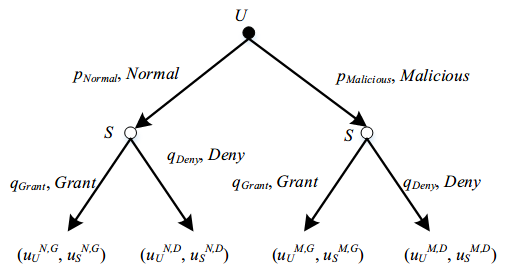
\includegraphics[width = 0.6\linewidth]{./figures/game-tree.png}
	\caption{风险自适应访问控制演化博弈模型的基本博弈树}
	\label{fig:game-tree}
\end{figure}

博弈参与者根据自身和其他参与者的策略选择而获取不同的数值收益,所有参与者的收益矩阵如表~\ref{tab:privacy-utilities-matrix}所示。

\begin{table}[htbp]
	\caption{风险自适应访问控制演化博弈模型的基本收益矩阵}
	\label{tab:privacy-utilities-matrix}
	\centering
	\begin{tabular}{cccc}%
		
		\toprule
		\textbf{ }&\textbf{ }&\multicolumn{2}{c}{信息资源系统~$S$~}\\
		\textbf{ }&\textbf{ }& ~$q_{Grant}$~,~$grant$~&~$q_{Deny}$~,~$Deny~$\\
		\midrule
		\multirow{2}{*}{用户~$U$~} & ~$p_{Normal}$~,~$Normal$~ &~$u_U^{N,G}$~, ~$u_S^{N,G}$~ & ~$u_U^{N,D}$~, ~$u_S^{N,D}$\\
		& ~$p_{Malicious}$~,~$malicious$~ &~$u_U^{M,G}$~, ~$u_S^{M,G}$~ & ~$u_U^{M,D}$~, ~$u_S^{M,D}$\\
		\bottomrule
	\end{tabular}
\end{table}

表~\ref{tab:privacy-utilities-matrix}中对演化博弈模型中各参与者的信念、策略和收益进行了形式化描述,特别的,参与者的收益根据访问请求的隐私风险不同而不同。


\begin{enumerate}
	\item  ~$u_{U}^{N,G}>0$~表示用户采用正常访问策略,被授权访问时的收益。该收益由正常访问获取工作职责完成的信息价值决定,并受到用户的隐私风险影响,用户的隐私风险越低其收益越高,反之越低,可表示为~$u_{U}^{N,G}=U_{Benefit}^{N,G}(r_{\max }^{U}-{{r}^{U}})$~,其中~$u_{Benefit}^{N,G}$~为用户采用正常访问策略被授权访问时的基础性收益,~$r_{\max }^{U}$~为用户的最大隐私风险,~${{r}^{U}}$~为用户的当前隐私风险。
	\item  ~$u_{U}^{N,D}=0$~表示用户采用正常访问策略,被拒绝访问时的收益,该值为0。
	\item  ~$u_{U}^{M,G}>0$~表示用户采用恶意访问策略,进行隐私侵犯访问被授权访问时的收益。该收益由用户正常访问的收益、隐私侵犯访问的额外收益组成,并受用户的隐私风险和当前访问请求的隐私风险影响。收益表示为~$u_{U}^{M,G}=U_{Benefit}^{N,G}(r_{\max }^{U}-{{r}^{U}})+U_{Extra}^{M,G}\cdot (r_{\max }^{U}-{{r}^{U}})\cdot r({{q}^{U}})$~,其中~$u_{Extra}^{M,G}$~为用户采用恶意访问策略被授权访问时的基础性额外收益。
	\item  ~$u_{U}^{M,D}<0$~表示用户采用恶意访问策略,进行隐私侵犯访问被拒绝访问时的收益。该收益是信息资源系统对用户的惩罚,并受到用户隐私风险和访问请求隐私风险的影响,风险值越大惩罚越大。该收益表示为~$u_{U}^{M,D}\text{=}U_{Punish}^{M,D}\cdot {{r}^{U}}\cdot r({{q}^{U}})$~,其中~$u_{Punish}^{M,G}$~是对用户在采取恶意访问策略时的基础性惩罚。
	\item  ~$u_{S}^{N,G}>0$~表示信息资源系统授权用户正常的访问请求时的收益。该收益是用户正常访问时完成工作职责时对系统的正向回馈,并受用户的隐私风险影响,用户隐私风险越低,系统收益越大。该收益可表示为~$u_{S}^{N,G}\text{=}S_{Benefit}^{N,G}(r_{\max }^{U}-{{r}^{U}})$~,其中~$s_{Benefit}^{N,G}$~为系统得到的基础性正向回馈。
	\item ~$u_{S}^{N,D}<0$~表示信息资源系统拒绝用户正常的访问请求时的收益。该收益是信息资源系统拒绝用户正常访问,无法完成用户工作职责而对系统造成的损失,用户的隐私风险越低,对系统的损失越大。该收益可表示为~$u_{S}^{N,D}\text{=}S_{Loss}^{N,D}(r_{\max }^{U}-{{r}^{U}})$~,其中~$s_{Loss}^{N,D}$~为系统受到的基础性损失。
	\item  ~$u_{S}^{M,G}<0$~表示信息资源系统授权用户恶意访问请求时的收益。该收益是被用户恶意访问所损失的隐私信息价值,受用户访问请求的隐私风险和用户隐私风险,风险值越大,信息资源系统的损失越大。该收益可表示为~$u_{S}^{M,G}\text{=}S_{Loss}^{M,G}\cdot {{r}^{U}}\cdot r({{q}^{U}})$~,其中~$s_{Loss}^{M,G}$~表示信息资源系统授权用户恶意访问时的基础性损失。
	\item ~$u_{S}^{M,D}=0$~表示信息资源系统拒绝用户的恶意访问时的收益。
\end{enumerate}

基于表~\ref{tab:privacy-utilities-matrix}可计算用户不同访问策略的期望收益和平均收益为
\begin{eqnarray}\label{eq:utilities-users}
u_{U}^{Normal}={{q}_{Grant}}u_{U}^{N,G}+{{q}_{Deny}}u_{U}^{N,D} \\ 
 u_{U}^{Malicious}={{q}_{Grant}}u_{U}^{M,G}+{{q}_{Deny}}u_{U}^{M,D} \\ 
{{\overline{u}}_{U}}={{p}_{Normal}}u_{U}^{Normal}+{{p}_{Malicious}}u_{U}^{Malic\text{i}ious}
\end{eqnarray}


由于风险访问收益较低者会学习模仿高收益者所选取的策略,针对用户可选策略集合~${{A}_{U}}=\{Normal,Malicious\}$~,选取不同策略的用户比例将随时间而发生变化,用~${{p}_{Normal}}(t)$~表示选取正常访问策略的用户比例,~${{p}_{Malicious}}(t)$~表示选取正常访问策略的用户比例,满足~${{p}_{Normal}}(t)\text{+}{{p}_{Malicious}}(t)\text{=}1$~。对于某一用户访问策略,选取该策略的用户比例是时间的函数,其动态变化速率可用复制动态方程表示。

\begin{equation}\label{eq:dynamic-equantion1}
D({{p}_{i}})=\frac{d{{p}_{i}}(t)}{dt}=p(u_{U}^{i}-{{\overline{u}}_{U}})
\end{equation}
其中~$i\in \{Normal,Malicious\}$~。
同理,

信息资源系统不同策略选择的期望收益和平均收益为

\begin{align}
& u_{S}^{Grant}={{p}_{Normal}}u_{S}^{N,G}+{{p}_{Malicious}}u_{S}^{M,G} \\ 
& u_{S}^{Deny}={{p}_{Normal}}u_{S}^{N,D}+{{p}_{Malicious}}u_{S}^{M,D} \\ 
& {{\overline{u}}_{S}}={{q}_{Grant}}u_{S}^{Grant}+{{q}_{Deny}}u_{S}^{Deny} \\ 
\end{align}
对信息资源系统的博弈策略选取亦可建立复制动态方程
\begin{equation}\label{eq:dynamic-equantion2}
A({{q}_{j}})=\frac{d{{q}_{j}}(t)}{dt}=q(u_{S}^{j}-{{\overline{u}}_{S}})
\end{equation}
其中~$j\in \{Grant,Deny\}$~。通过联立式~\ref{eq:dynamic-equantion1}和~\ref{eq:dynamic-equantion2},令
\begin{equation}\label{eq:differential-equation}
Y=[ D(p), A(q)]'=f(Y,t)=0
\end{equation}
可求解公式~\ref{eq:differential-equation},即可得到隐私风险访问模型的演化博弈平衡状态点,从而实现访问控制策略选取的分析和预测。



\subsection{博弈演化稳定策略均衡求解}
\label{subsec:solution}
所提出的隐私风险访问控制模型中,用户选取不同的访问行为策略会产生不同的收益,收益低的用户会模仿收益高的用户所选取的访问行为策略。对于相同工作职责的~$n$~个用户,有两种访问策略~$\{Normal, Malicious\} ~$~可选,选取这两种访问策略的用户比例随着时间发生变化,分别为~$p_{Normal}(t)$~和~$1-p_{Normal}(t)$~。对于访问策略~$Normal$~,选取该策略的用户人数比例是时间的函数,其动态变化速率可表示为动态复制函数

\begin{equation}\label{eq:dynamic-equations}
D({{p}_{Normal}})=\frac{d{{p}_{Normal}}(t)}{dt}={{p}_{Normal}}(u_{U}^{Normal}-{{\overline{u}}_{U}})
\end{equation}

 令~$D({{p}_{Normal}})=0$~,将式~\ref{eq:utilities-users}代入~\ref{eq:dynamic-equations}可求解,得~${{p}_{Normal}}=0$~,~${{p}_{Normal}}\text{=}1$~和~${{q}_{Grant}}=\\\frac{u_{U}^{M,D}-u_{U}^{M,G}}{u_{U}^{N,G}-u_{U}^{N,D}\text{-}u_{U}^{M,G}\text{+}u_{U}^{M,D}}$~。
 
 类似地,信息资源系统的两种可选行为策略~$\{Grant,Deny\}$~及其策略选取概率~$q_{Grant}(t)~$和~$1-q_{Grant}(t)$~,对于策略Grant的选取概率时间变化函数,亦可求解得~$q=0$~,~$q=1$~和~${{p}_{Normal}}=\frac{u_{S}^{M,D}-u_{S}^{M,G}}{u_{S}^{N,G}-u_{S}^{N,D}\text{-}u_{S}^{M,G}\text{+}u_{S}^{M,D}}$~。

将用户与信息资源系统的策略选取复制动态方程相结合,构建隐私风险访问控制演化博弈方程组,对博弈模型进行稳定性分析。求解方程组得5个解 ~${{Y}_{1}}=[0,1]'$~,~${{Y}_{2}}=\left[ 0 ,1 \right]'$~,~${{Y}_{3}}=\left[1 ,0 \right]'$~,~${{Y}_{4}}=\left[ 1 ,1 \right]'$~和~${{Y}_{5}}=
\begin{bmatrix}
\frac{u_{S}^{M,D}-u_{S}^{M,G}}{u_{S}^{N,G}-u_{S}^{N,D}\text{-}u_{S}^{M,G}\text{+}u_{S}^{M,D}},
\frac{u_{U}^{M,D}-u_{U}^{M,G}}{u_{U}^{N,G}-u_{U}^{N,D}\text{-}u_{U}^{M,G}\text{+}u_{U}^{M,D}}
\end{bmatrix}'$~。其中,~${{Y}_{1}}=[0,1]'$~表示用户选取纯策略恶意访问请求~$malicious$~,信息资源系统选取纯策略拒绝访问~$Deny$~;~${{Y}_{2}}=\left[ 0 ,1 \right]'$~表示用户纯策略选取恶意访问请求~$malicious$~,信息资源系统选取纯策略允许访问~$grant$~;~${{Y}_{3}}=\left[1 ,0 \right]'$~表示用户纯策略选取正常访问请求~$Normal$~,信息资源系统选取纯策略拒绝访问~$Deny$~;~${{Y}_{4}}=\left[ 1 ,1 \right]'$~表示用户纯策略选取正常访问请求~$Normal$~,信息资源系统选取纯策略允许访问~$grant$~;~${{Y}_{5}}=
\begin{bmatrix}
\frac{u_{S}^{M,D}-u_{S}^{M,G}}{u_{S}^{N,G}-u_{S}^{N,D}\text{-}u_{S}^{M,G}\text{+}u_{S}^{M,D}},
\frac{u_{U}^{M,D}-u_{U}^{M,G}}{u_{U}^{N,G}-u_{U}^{N,D}\text{-}u_{U}^{M,G}\text{+}u_{U}^{M,D}}
\end{bmatrix}'$~表示用户以混合概率组合~$( \frac{u_{S}^{M,D}-u_{S}^{M,G}}{u_{S}^{N,G}-u_{S}^{N,D}\text{-}u_{S}^{M,G}\text{+}u_{S}^{M,D}}, 1- \frac{u_{S}^{M,D}-u_{S}^{M,G}}{u_{S}^{N,G}-u_{S}^{N,D}\text{-}u_{S}^{M,G}\text{+}u_{S}^{M,D}})$~选取策略~$\{Normal, Malicious\}$~,信息资源系统以混合概率组合~$(\frac{u_{S}^{M,D}-u_{S}^{M,G}}{u_{S}^{N,G}-u_{S}^{N,D}\text{-}u_{S}^{M,G}\text{+}u_{S}^{M,D}} , 1-\frac{u_{S}^{M,D}-u_{S}^{M,G}}{u_{S}^{N,G}-u_{S}^{N,D}\text{-}u_{S}^{M,G}\text{+}u_{S}^{M,D}} )$~选取策略~$\{Grant, Deny\}$~。根据演化稳定策略理论可知~$Y_1$~、~$Y_2$~、~$Y_3$~、~$Y_4$~为鞍点,~$Y_5~$~为中心点,故所提出的风险自适应访问控制演化博弈模型存在演化稳定均衡。

\subsection{博弈演化稳定策略分析}
演化稳定策略是演化博弈模型中能够抵抗侵犯的策略。在所提出的风险自适应访问控制演化博弈模型中,用户和信息资源系统双方各自存在复制动态,以用户为例,对其演化稳定策略进行分析。通过式~\ref{eq:dynamic-equations}可知,用户正常访问请求策略选取的复制动态相位有3种,当~${{q}_{Grant}}=\frac{u_{U}^{M,D}-u_{U}^{M,G}}{u_{U}^{N,G}-u_{U}^{N,D}\text{-}u_{U}^{M,G}\text{+}u_{U}^{M,D}}$~时,对任意的用户正常访问请求~$Normal$~策略选取概率~$p_{Normal}$~,有~$\frac{d{{p}_{Normal}}(t)}{dt}\text{=0}$~,但是一旦~$q_{Grant}$~的取值发生偏移,~$\frac{d{{p}_{Normal}}(t)}{dt}$~就会剧烈变化,其所代表的状态不具有稳定性;当~${{q}_{Grant}}>\frac{u_{U}^{M,D}-u_{U}^{M,G}}{u_{U}^{N,G}-u_{U}^{N,D}\text{-}u_{U}^{M,G}\text{+}u_{U}^{M,D}}$~时,~$p_{Normal}= 1$~为用户的演化稳定策略;当~${{q}_{Grant}}<\frac{u_{U}^{M,D}-u_{U}^{M,G}}{u_{U}^{N,G}-u_{U}^{N,D}\text{-}u_{U}^{M,G}\text{+}u_{U}^{M,D}}$~时,~$p_{Normal}=0$~为用户的演化稳定策略。

 同理,信息资源系统授权策略选取的复制动态相位有3种,当~${{p}_{Normal}}=\frac{u_{S}^{M,D}-u_{S}^{M,G}}{u_{S}^{N,G}-u_{S}^{N,D}\text{-}u_{S}^{M,G}\text{+}u_{S}^{M,D}}$\\时,对任意的授权访问策略选取概率~$q_{Grant}(t)$~,有~$\frac{d{{q}_{Grant}}(t)}{dt}\text{=0}$~,该状态不具有稳定性;当~${{p}_{Normal}}>\frac{u_{S}^{M,D}-u_{S}^{M,G}}{u_{S}^{N,G}-u_{S}^{N,D}\text{-}u_{S}^{M,G}\text{+}u_{S}^{M,D}}$~时,~$q_{Grant}(t)=1$~是信息资源系统的演化稳定策略;当~${{p}_{Normal}}<\frac{u_{S}^{M,D}-u_{S}^{M,G}}{u_{S}^{N,G}-u_{S}^{N,D}\text{-}u_{S}^{M,G}\text{+}u_{S}^{M,D}}$~时,~$q_{Grant}(t)=0$~是信息资源系统的演化稳定策略。
 
 
 \section{实验仿真与分析}
本节对本章提出的隐私风险自适应访问控制模型的演化博弈过程,利用动力学理论进行仿真,分析隐私风险自适应访问控制演化博弈模型的最优访问策略选取问题。

 由~\ref{subsec:solution}节可知,该访问控制模型的演化博弈稳定状态为~${{Y}_{1}}=[0,0]'$~,~${{Y}_{2}}=[0,1]'$~,~${{Y}_{3}}=[1,0]'$~和~${{Y}_{4}}=[1,1]'$~,下面针对 和 的不同初始状态,进行实验仿真。通过仿真可以看出~$p_{Normal}$~和~$q_{Grant}$~的演化趋势,得到最终的演化稳定状态,通过演化分析,实现隐私风险访问控制系统中参与者的策略选择预测,从而选取出最优的访问控制策略。本章的仿真实验中,根据~\ref{subsec:evolutionary-game-model}节中的分析对用户的效用函数设定为~$u_{U}^{N,G}>u_{U}^{M,G}>u_{U}^{N,D}>u_{U}^{M,D}$~,对信息资源系统的效用函数设定为~$u_{S}^{N,G}>u_{S}^{M,D}>u_{S}^{N,D}>u_{S}^{M,G}$~。

\begin{enumerate}
 	\item 当初始状态为~${{p}_{Normal}}\text{=0}$~,~${{q}_{Grant}}\in [0,1)$~时,用户以概率1选取恶意访问~$Normal$~策略,信息资源系统以概率1选取拒绝访问Deny策略或任意其他混合策略选取授权访问~$Grant$~、拒绝访问~$Deny$~策略,通过系统仿真,经过演化,用户和信息资源系统双方的策略选取都会演化为~${{p}_{Normal}}\text{=0}$~,~${{q}_{Grant}}=0$~的概率,即用户以纯策略选取恶意访问~$Malicious$~,信息资源系统以纯策略选取拒绝访问~$Deny$~。~${{p}_{Normal}}$~和~${{q}_{Grant}}$~的具体演化曲线如图~\ref{fig:Evolutionary-exp1}所示,在达到演化稳定状态~${{Y}_{1}}=[0,0]'$~时,风险自适应访问控制演化博弈模型的博弈参与者两方博弈策略选取最优。
 	
 	 \begin{figure}[htbp]
 		\centering
 		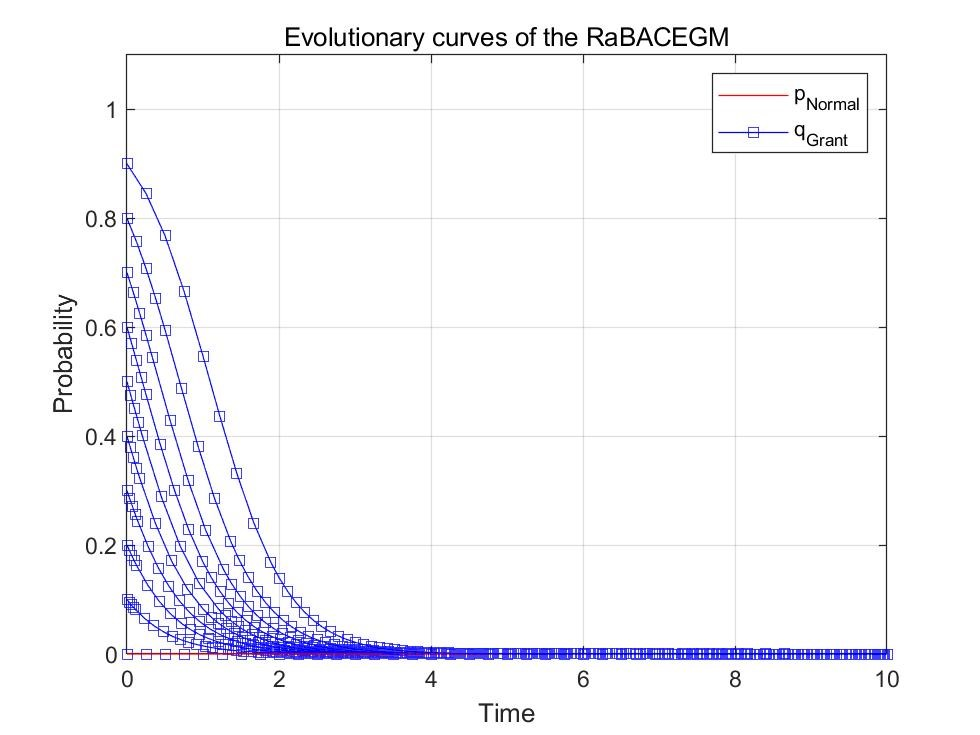
\includegraphics[width=0.8\linewidth]{./figures/Evolutionary-exp1.jpg}
 		\centering
 		\caption{初始状态为~$p_{Normal}=0,q_{Grant}\in [1,0)$~时,隐私风险自适应访问控制演化博弈模型的演化曲线,演化稳定状态为~$p_{Normal}=0, q_{Grant}=0$~}\label{fig:Evolutionary-exp1}
 	\end{figure}
 
 	\item 当初始状态为~${{p}_{Normal}}\text{=0}$~,~${{q}_{Grant}}\text{=}1$~时,用户以概率1选取恶意访问~$Malicious$~策略,信息资源系统以概率1选取授权访问~$Grant$~策略,通过演化,该演化博弈模型的博弈双方的策略选取不变,~${{p}_{Normal}}$~和~${{q}_{Grant}}$~的具体演化曲线如图~\ref{fig:Evolutionary-exp2}所示。
 	
 	 \begin{figure}[htbp]
 		\centering
 		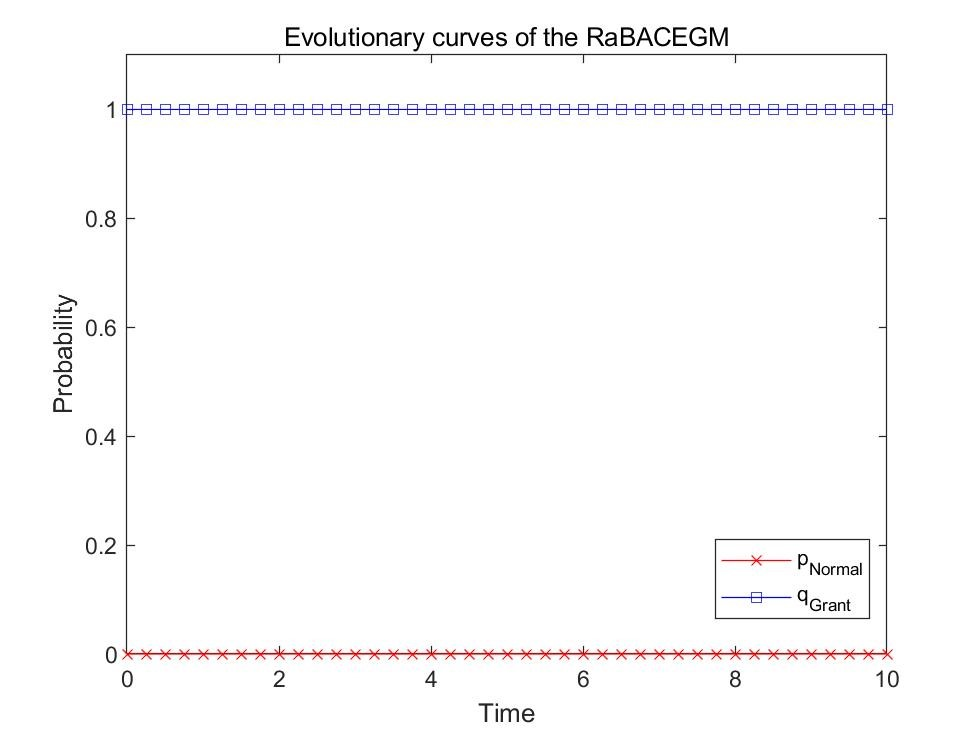
\includegraphics[width=0.8\linewidth]{./figures/Evolutionary-exp2.jpg}
 		\centering
 		\caption{初始状态为~$p_{Normal}=0, q_{Grant}=1$~时,隐私风险自适应访问控制演化博弈模型的演化曲线,演化稳定状态为~$p_{Normal}=0, q_{Grant}=1$~}\label{fig:Evolutionary-exp2}
 	\end{figure}
 
 		在图~\ref{fig:Evolutionary-exp2}中,尽管该演化过程的最终状态~${{Y}_{2}}=[0,1]'$~是所提出的演化博弈模型的演化稳定状态,但在实际应用中,信息资源系统为了遏制恶意访问请求,保护系统中的隐私数据,同时尽可能吸引更多用户访问系统,其不会以纯策略方式选取授权访问~$Grant$~,故当用户初始访问策略选取为纯策略恶意访问~$Malicious$~时,会转换为图~\ref{fig:Evolutionary-exp1}所示的演化曲线。
 		
 	\item 当初始状态为~${{p}_{Normal}}\in (0,1]$~,~${{q}_{Grant}}\in (0,1]$~时,用户以混合策略方式选取正常访问~$Normal$~、恶意访问~$Malicious$~,或以纯策略方式(概率为1)选取正常访问~$Normal$~,信息资源系统以混合策略方式选取授权访问~$Grant$~、拒绝访问~$Deny$~,或以纯策略方式(概率为1)选取拒绝访问~$Deny$~,博弈模型通过不断演化,会达到演化稳定状态~${{Y}_{4}}=[1,1]'$~,即用户以纯策略方式选取正常访问~$Normal$~,信息资源系统以混合策略方式选取授权访问~$grant$~。该状态下风险自适应访问控制演化博弈模型的博弈策略选择最优,~${{p}_{Normal}}$~和~${{q}_{Grant}}$~的演化曲线如图~\ref{fig:Evolutionary-exp4}所示。
 	
 	\begin{figure}[htbp]
 		\centering
 		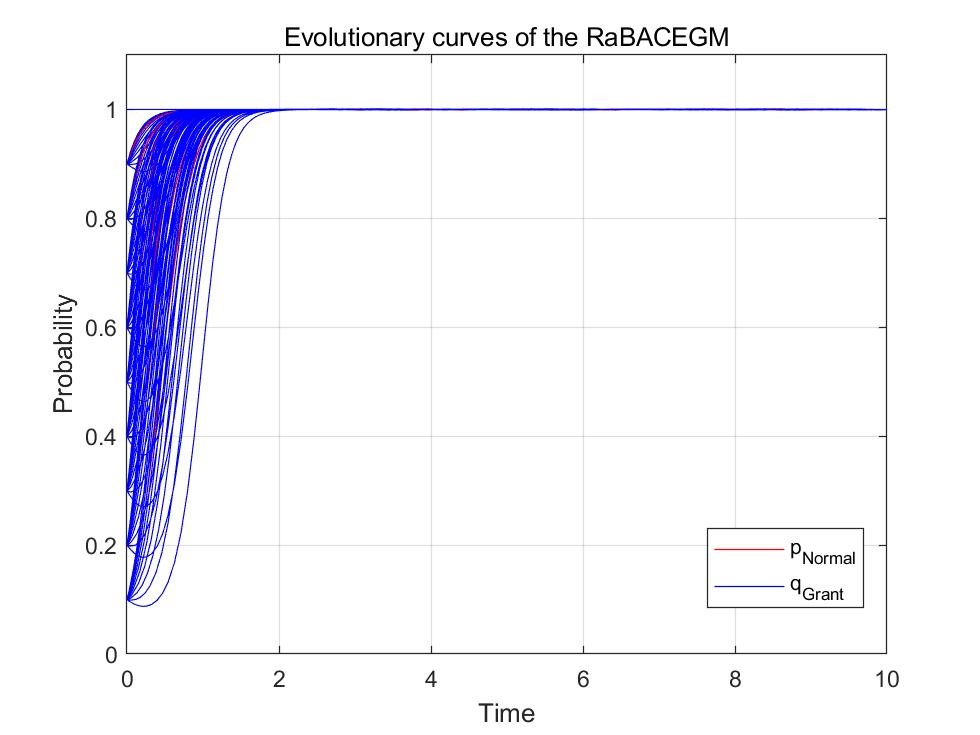
\includegraphics[width=0.8\linewidth]{./figures/Evolutionary-exp3.jpg}
 		\centering
 		\caption{初始状态为~$p_{Normal}\in (0,1]$~,~$q_{Grant}\in (0,1]$~时,隐私风险自适应访问控制演化博弈模型的演化曲线,演化稳定状态为~$p_{Normal}=1$~,~$q_{Grant}=1$~}\label{fig:Evolutionary-exp3}
 	\end{figure}
 
 	\item 当初始状态为~${{p}_{Normal}}\in (0,1]$~,~${{q}_{Grant}}\text{=}0$~时,用户以混合策略方式选取正常访问~$Normal$~、恶意访问~$Malicious$~,或以纯策略方式(概率为1)选取正常访问~$Normal$~,信息资源系统以纯策略方式(概率为1)选取拒绝访问~$Deny$~,通过不断演化,会达到演化稳定状态~${{p}_{Normal}}\text{=}1$~,~${{q}_{Grant}}\text{=}0$~,即用户以纯策略方式选取正常访问~$Normal$~,信息资源系统以纯策略方式选取拒绝访问~$Deny$~。~${{p}_{Normal}}$~和~${{q}_{Grant}}$~的具体演化曲线如图~\ref{fig:Evolutionary-exp4}所示。
 	
 	\begin{figure}[htbp]
 		\centering
 		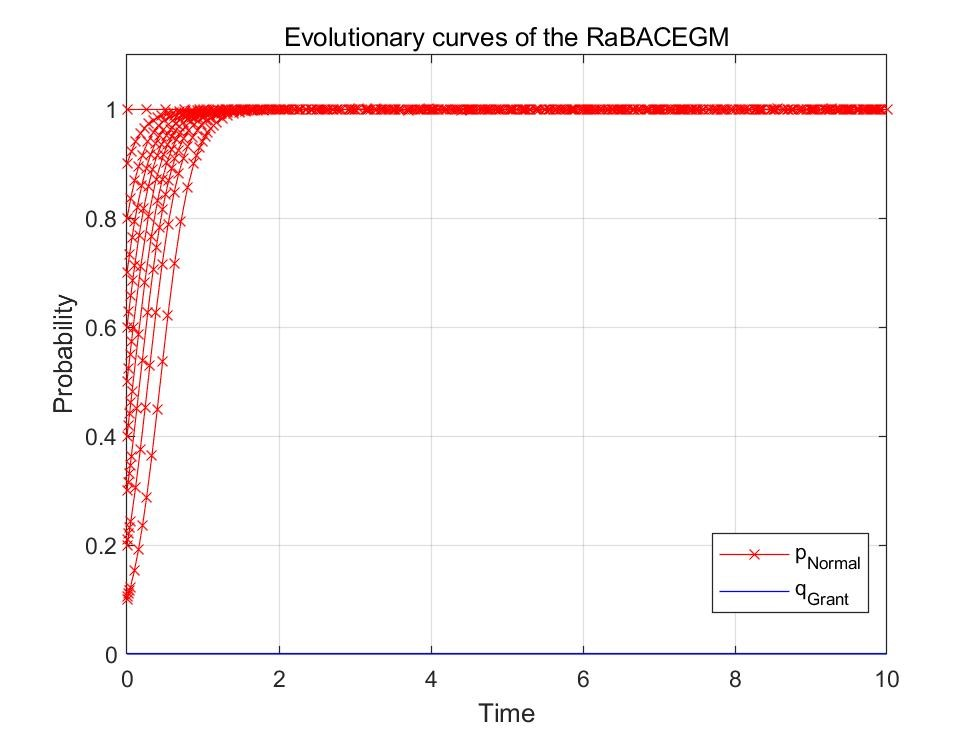
\includegraphics[width=0.8\linewidth]{./figures/Evolutionary-exp4.jpg}
 		\centering
 		\caption{初始状态为~$p_{Normal}\in(0,1],q_Grant=0$~时,隐私风险自适应访问控制演化博弈模型的演化曲线,演化稳定状态为~$p_{Normal}=1,q_{Grant}=0$~}\label{fig:Evolutionary-exp4}
 	\end{figure}
 	
 	在图~\ref{fig:Evolutionary-exp4}中,最终达到的演化状态是风险自适应访问控制演化博弈模型的演化稳定状态~${{Y}_{3}}=[10]'$~。但在实际应用中,信息资源系统为了吸引更多用户访问系统,其不会以纯策略方式选取拒绝访问Deny,会以混合策略的方式选取其博弈策略,其演化过程会转换为图~\ref{fig:Evolutionary-exp3}所示的演化曲线。
 \end{enumerate}


 由以上仿真结果可知,给定不同的策略选取初始状态,经过演化,所提出的风险自适应访问控制模型在演化博弈过程中会达到某个稳定状态。通过对比,本演化博弈模型的模拟演化结果与第~\ref{sec:evolutionary-game-model}节中的理论分析保持一致,说明该演化博弈模型与现实系统中的规律相符。因此,本章提出的风险自适应访问控制演化博弈模型具有有效性,可将其应用于面向隐私保护的风险自适应访问控制系统中,为访问控制系统的参与者进行隐私保护访问策略选取提供依据。
 
 \section{对比与讨论}
 
 在风险访问控制、基于博弈的访问控制和基于演化博弈的信息安全模型方面均有相应的研究,本节针对这些研究工作进行对比,如表~\ref{tab:game-model-comparision}所示。
\begin{table}[htbp]
	\caption{所提出风险自适应访问控制模型的对比}
	\label{tab:game-model-comparision}
	\centering
	\begin{tabular}{ccccc}%
		
		\toprule
		文献  &	访问控制目的&	风险量化&	博弈参与者&	博弈方法\\
		\midrule
		文献~\cite{ni2010risk}&
		安全保护&	静态安全风险量化&	-&	-\\
		文献~\cite{shaikh2012dynamic}&
		安全保护&	风险和信任动态量化&	-&	-\\
		文献~\cite{santos2016framework}&
		云安全保护&	多因子聚合风险量化&	-&	-\\
		文献~\cite{wang2011quantified}&
		医疗信息隐私保护&	静态隐私风险量化&	-&	-\\
		文献~\cite{zhang2018privacy}&
		医疗信息隐私保护&	动态隐私风险量化\\		
		文献~\cite{gao2018game}&
		云安全保护&	-&	二参与者&	重复博弈\\
		文献~\cite{liu2016dynamic}&
		蜂窝网络接入安全&	-	&多参与者&	Stackelberg博弈\\
		文献~\cite{helil2017non}&
		数据安全&	动态安全风险量化&	二参与者&	非零和合作博弈\\
		文献~\cite{hu2014game}&
		社交网络隐私保护&	静态隐私风险量化&	多参与者&	多方控制博弈\\
		本章&	敏感数据隐私保护&	隐私风险自适应量化&	多参与者&	演化博弈\\
	
		\bottomrule
	\end{tabular}
\end{table}

由表~\ref{tab:game-model-comparision}可知,相较于文献~\cite{ni2010risk,shaikh2012dynamic,santos2016framework},本章所提出的风险访问控制从系统安全保护扩展至数据隐私信息保护,同时在有限理性假设下,应用多人演化博弈对自适应风险访问控制的参与者群体进行了建模和分析;相较于文献~\cite{wang2011quantified,zhang2018privacy},本章将隐私保护的应用范围推广至一般以隐私数据为中心的系统中,并利用博弈论对隐私保护的访问策略选择进行了分析;相较于文献~\cite{gao2018game,liu2016dynamic},本章不关注系统的安全,而关注于系统中的敏感数据隐私保护,通过隐私风险量化对博弈的效用函数进行定义,且放松了对博弈参与者的绝对理性假设,用演化的思想动态分析参与者的访问策略选择;相较于文献~\cite{helil2017non},本章的主要目标是隐私保护,将传统访问控制的二人博弈扩展为有限理性下的多人动态博弈,更加适用于访问控制的真实场景,风险量化函数也通过信息量的量化对隐私风险进行描述,并反映到博弈效用函数中;相较于文献~\cite{hu2014game},本章不局限于特定场景的隐私保护,其适用于通用的隐私保护场景,并且通过对用户隐私风险和访问请求隐私风险进行动态量化,实现了隐私风险自适应。在多人博弈场景中,对参与者的理性假设放松为有限理性,利用演化的思想对参与者的策略选择进行动态更新,更加符合现实场景中参与者的访问行为变化特征。
 \section{小结}
隐私保护是以数据为中心的开放系统的核心问题之一,设计有效的细粒度自适应访问控制模型能够保护系统中的隐私数据不被恶意、好奇的访问行为侵犯隐私。本章面向隐私保护,在有限理性假设下,提出了一种基于演化博弈的隐私风险自适应访问控制模型,该模型利用隐私信息量化的方法对访问请求隐私风险和用户隐私风险进行量化,在此基础上构建了两方群体的演化博弈模型,群体中博弈参与者不断学习模仿高收益的参与者博弈策略,最终达到演化稳定状态。通过复制动态方程分析了所提出的风险自适应访问控制演化博弈模型中参与者的策略选择变化过程和演化稳定状态形成机理,提出了演化稳定策略的求解公式。通过仿真实验,对所提出自适应隐私风险访问控制模型的有效性进行了验证,该模型能有效应用于隐私保护的访问控制;通过与相关文献对比,该模型提出了新的隐私风险自适应量化方法,减少了对系统历史信息的要求,具有更好的隐私风险动态适应性,并将自适应隐私风险量化结果用以设计演化博弈的效用函数;提出了有限理性多参与者的风险访问控制演化博弈模型,该模型中参与者的博弈策略选择动态更新,更适用于真实场景。%结论
\chapter{总结及展望}
\label{chap:conclusions}


\section{结论}
互联网、移动互联网和物联网快速发展,以及5G技术的不断推进和商用推广,社交网络、位置服务、医疗健康、生物基因、工业控制等海量数据被主动或被动采集、传输、存储、流转、分析并应用。数据海量化增长、网络跨域泛在、计算云端化、应用多样复杂化等新的变化为安全和隐私带来了巨大挑战,大量的病毒、漏洞、攻击和数据关联分析,致使隐私严重泄漏,引发了人们极大的担忧。如何对隐私进行恰当的定义与度量,如何深入的对隐私进行分析与推测以提高对隐私的认识与理解,如何设计更加有效动态的隐私保护机制,实现隐私保护与数据效用的平衡,称为亟待解决的问题。

面对隐私领域的隐私定义与度量、隐私分析与推断、以及隐私保护算法的研究需求和挑战,本文主要针对数据开放共享场景下的基于非密码学隐私研究,展开了隐私度量、隐私分析、隐私保护及隐私保护与数据效用平衡方面研究,深入探究了隐私的基础理论,提出了能够对隐私定义量化、隐私分析强度量化、隐私保护机制能力量化的统一信息论框架模型;针对数据共享应用中序列型数据的属性隐私提出了不同模式的隐私分析概率推断模型和算法,提高了对隐私泄露及隐私保护机理的理解;提出能够动态、自适应地对包含大量隐私信息的数据集进行隐私保护风险访问控制模型,并进一步结合两方博弈和群体博弈,提出了基于博弈论的理性隐私风险访问控制模型,实现了隐私保护与数据效用间的平衡。取得了如下进展与结论:
\begin{enumerate}
	\item 基于Shannon信息论的通信模型框架提出了几种隐私保护信息通信模型,对不含敌手的隐私保护、含敌手的隐私保护、多隐私保护源的隐私保护等不同情境提出了相应的模型进行建模,以满足对隐私度量、隐私保护机制效果度量和敌手隐私分析强度度量等需求。在所提出的度量模型中,将信息拥有者假设为发送方,隐私谋取者假设为接收方,隐私的泄露渠道假设为通信信道;基于该假设,分别引入信息熵、平均互信息量、条件熵及条件互信息来分别描述隐私保护系统信息源的隐私度量、隐私泄露度量、含背景知识的隐私度量及泄露度量,形成了以信息论为核心的隐私度量方法体系;以此为基础,进一步提出了隐私保护方法的强度和敌手攻击强度的量化,为隐私泄露的量化提供了一种支撑,对整个隐私保护过程中的保护机制、敌手能力都提供了量化方法。%;最后,针对位置隐私保护的应用场景,通过所提出的隐私信息通信模型给出了具体的信息熵模型、以及隐私保护机制和攻击强度的度量及分析。
	
	\item 针对基因序列数据的基因属性隐私提出了一种基于概率推断的隐私分析模型。该模型通过对单条敏感数据记录属性值存在的相互关联关系进行分析,构建目标属性值推断的敌手模型。在提出的敌手模型基础上,分别提出了两种不同的基因序列属性隐私分析方法。第一种主要基于蒙克卡罗-Markov抽和隐Markov推断算法,建立了目标基因序列的“抽样解析”——“单倍体属性值概率推断”——“二倍体合成”三个步骤的属性隐私推断模型;第二种方法应用卷积神经网络构建概率推断算法,改进了单倍体属性值推断过程,实现了大规模序列型数据的属性推断目标。所提出的方法针对不存在亲属关系的群体型基因序列数据共享场景,在所提出的隐私度量模型基础上,定义了序列型数据属性隐私和量化方法,并应用于分析属性隐私泄露情况,通过量化隐私泄露量和敌手获取隐私量等信息,提高对序列型数据属性隐私的认识和理解。实验表明,提出的方法比现有基因序列属性隐私分析模型和算法更优,敌手对属性隐私的错误率、不确定度降低,敌手获得隐私信息量都比已有的工作更优。
	\item 针对家族成员基因序列数据共享会造成他人基因序列属性隐私泄露无法量化的问题,利用因子图和置信传播算法针对亲属间的基因序列属性隐私建立分析推断敌手模型和分析算法,提高了亲属基因组属性隐私推断攻击的准确性。该模型考虑了单核苷酸多态性间高阶相关关系,利用公开DNA参照数据集和全基因组关联研究(GWAS)目录数据,提高了推断攻击模型的属性隐私分析强度。实验结果表明,所提出的攻击更适合于高密度基因组数据隐私推断,且具有较少的不正确性、不确定性和更多隐私损失,显著提高了关联性基因数据属性隐私的推断能力。
	\item 针对云环境中共享、应用涉及隐私或敏感信息数据的场景研究面向隐私保护的访问控制模型。在XACML上扩展提出了一种基于风险的自适应访问控制模型,以动态化在访问控制过程中保护数据隐私,约束隐私侵犯行为,激励诚实访问行为。首先,根据风险访问控制场景的隐私保护需求提出了面向隐私保护的风险访问控制敌手模型该;其次,该模型在标准的XACML框架基础上进行了扩展,改进了策略风险评估、会话控制和风险消减服务三个组件,增强了策略执行、策略访问和策略信息组件。在新增的组件中,以Shannon信息熵作为工具,在所提出的隐私度量模型基础上,提出了基于风险的隐私定义和量化方法,对用户的访问控制请求风险和用户自身的风险类型结合,提出了访问请求类型判别方法;通过风险隐私量化及基于信誉的激励机制,实现访问行为风险阈值的动态调整,考虑了用户短期访问行为和长期访问行为的影响。对比和分析表明,所提出的模型和方法较现有的工作更加动态化,且实现了隐私保护,易用性更好。
	
	\item 在所提出的风险自适应访问控制模型的基础上,进一步运用Shannon信息和博弈论,提出了基于风险适应性的理性访问模型以实现数据共享场景中的保护隐私和数据应用需求间的平衡。在定义了隐私风险和隐私侵犯访问的概念之后,提出了基于博弈论风险的访问控制模型框架和工作流程。此外,还进一步改利用Shannon信息的定义提出了量化访问请求和用户的隐私风险值计算公式,强化了访问控制请求对数据隐私的刻画;以所提出的理性风险访问控制模型、访问请求隐私 风险和用户隐私风险为基础,提出了多轮二人博弈来刻画面向隐私保护的风险访问控制中访问者与数据服务提供者的”隐私保护-数据服务“冲突与合作关系,进一步提出并分析了博弈效用函数及其二人博弈过程。分析表明,在基于风险的访问控制的每一轮博弈中都存在子博弈精炼Nash均衡,可以通过限制侵犯隐私的访问请求来保护隐私。分析和比较表明,该方法比已有的工作更有优势,需要更少的辅助信息,提供更多的风险适应性和隐私保护强度。
	
	\item 在提出的风险自适应访问控制模型和两方理性隐私风险访问控制模型的基础上,进一步提出一种面向隐私保护的多参与者理性风险自适应访问控制模型。新提出的模型包含了新的隐私风险量化模块和演化博弈决策模块。该模型首先基于Shannon信息对访问请求的数据集隐私信息量进行量化,基于Markov模型构造了访问请求隐私风险函数和用户隐私风险函数;其次,基于演化博弈在有限理性假设下构建多参与者的访问控制演化博弈模型,利用复制动态方程分析了访问控制参与者的动态策略选择和演化稳定状态形成机理,提出了隐私风险访问控制博弈演化稳定策略的选取方法。仿真实验和对比表明,所提出的访问控制模型能够有效动态自适应地保护敏感信息资源系统中的隐私信息,具有更好的隐私风险适应性,有限理性参与者的动态演化访问策略选取更加符合实际场景。
	
\end{enumerate}

\section{展望}
   本文围绕数据共享应用场景中的隐私度量、隐私分析和隐私保护几个问题进行了研究,研究成果对于以数据为中心的开放型系统的隐私保护发展有一定的理论和应用价值。然而,由于数据类型的多样化和海量化,应用场景的复杂化和跨域化,仍会出现更多的隐私问题。因此,我们对本文的工作进行简要展望:
\begin{enumerate}
	\item 在隐私度量方面,研究隐私分析强度与隐私保护强度的统一度量问题。目前提出的隐私度量方法,不能有效的将隐私定义、隐私分析强度和隐私保护强度三方面统一可转换的方法进行量化。如何设计能有效对三者进行关联性度量的方法是一个值得研究的课题。如何用更加有效的基础理论,如结构信息论对图结构数据、复杂网络数据的隐私进行量化和分析,也非常值得研究。
	
	\item 在隐私分析方面,研究更加有效的隐私推断模型,以更深入地理解隐私。如何对更加多样化的场景,如社交网络、数据挖掘、机器学习、外包计算等场景下的匿名隐私、关系隐私和属性隐私进行可迭代式的推断分析,值得研究。
	
	\item 在隐私保护与数据效用平衡方面,研究匿名隐私、关系隐私、属性隐私等不同隐私需求与数据效用的可交换型隐私保护方案,研究基于博弈的跨域多用户隐私与效用公平性分配问题,是有意义的研究点。

\end{enumerate}
%结论
%%%%%%%%%%%%%%%%%%%%%%%%%%%%%%
%% 附件部分
%%%%%%%%%%%%%%%%%%%%%%%%%%%%%%
\backmatter

%%%%%%%%%%%%%%%%%%%%%%%%%%%%%%%%%%参考文献%%%%%%%%%%%%%%%%%%%%%%%%%%%%%%%%%%%%%%%%%
%\bibliographystyle{gbt7714-unsrt}
\bibliography{thesis-references}
%%%%%%%%%%%%%%%%%%%%%%%%%%%%%%%%%%%%%%%%%%%%%%%%%%%%%%%%%%%%%%%%%%%%%%%%%%%%% 摘要


%%%%%%%%%%%%%%%%%%%%%%%%%%%%%%%%%%%%%%%%%%%%%%%%%%%%%%% 致谢%%%%%%%%%%%%%%%%%%%%%%%%%%%%%%%%%%%%%
\begin{thanks}
	
	在论文完成之际,有需要很多人值得感谢。
	首先感谢我的家人,感谢父母的养育与理解,给了我足够的空间让我来做我自己想做的事,给了我足够的支持让我不断进取;感谢兄弟姐妹的包容和理解,他们承担的更多家庭责任,才让我有了选择攻读学位的机会。
	
	其次,感谢我的导师向淑文教授和彭长根教授,向老师对问题本质的深刻认识和理解,在关键时刻和核心问题上一针见血地指出论文的研究方向;彭老师在选题、具体研究、论文写作等各阶段都付出了大量的时间和精力,彭老师对论文的指导遍布了实验室、办公室、组会、操场、车上、飞机上、学术会议现场……有了这些,才有该论文的成果。两位老师崇高的学术精神和对科学问题追根溯源的态度都深刻影响了我,对论文的完成也至关重要,下一步还将沿着两位老师指导的方向,继续沿着科学的道路前行。
	
	再次,感谢田有亮教授,感谢他在论文写作过程中的反复讨论,感谢他在论文各章成果小论文写作、发表过程中的意见、讨论和帮助,学位论文的完成也得到他的多次指点。感谢实验室的师兄弟姐妹们,在一起相互学习生活了几年美好的时光,一起讨论科学问题、一起吃烧烤、一起开玩笑……这些将成为我一生的宝贵经历。也感谢大家在论文初稿完稿时,帮助我读论文、改词句,对论文的质量和可读性提高都起到了非常大的作用。
	
	感谢在Leigh访学期间的合作导师Yinzhi Cao教授以及实验室的同学们,感谢在一起讨论问题、写作方法、发论文的感受,感谢他们让我对科研方法有了新的认识,也感谢在一起对网络隐私和移动隐私有了新的理解。
	
	也感谢学院的各位老师,完成本文工作也得到了他们的很多支持,感谢杨辉教授,无论是论文开题研究还是日常工作,都得到杨老师的诸多帮助;感谢吴妍妍、何飞、贺亚琼、夏正香、李永钗等各位老师,每次到学院办公室都是要麻烦他们,他们的帮助总是非常温暖。感谢刘圣达同学贡献的学位论文Latex模板,免去了我写作过程中繁琐的格式与排版工作。
	
	感谢所有支持此篇论文完稿的人。
	
	
\end{thanks}%结论


%%%%%%%%%%%%%%%%%%%%%%%%%%%%%%%%%%%%%%%%%%%%%%%%%%%%%%%%攻读学位期间科研和论文情况%%%%%%%%%%%%%%%
\newpage
\Nchapter{攻读博士学位期间科研和论文情况}  %博士同学请注意修改此标题

\begin{resumesection}{一、科研工作}

\textbf{主持科研项目:}\\
1. 贵州大学研究生创新基金:大数据环境下的风险自适应隐私保护访问控制模型及其应用研究(No.研理工2016068)

\textbf{参与科研项目:}\\
1. 国家自然科学基金重点项目:数据共享应用的块数据融合分析理论与安全管控模型研究(No. U1836205)\\
2. 国家自然科学基金地区项目:理性隐私计算及隐私风险可控技术研究(No. 61662009)\\
3.  国家自然科学基金面上项目:理性委托计算的可组合安全理论及其构造方法研究(No.61772008)\\
4. 贵州省科技计划重大专项:面向多源法院数据融合的数据安全防护与隐私保护算法及模型研究(No. 黔科合重大专项字[2017]3002)\\
5. 贵州省科技计划重大专项:大数据安全与隐私保护关键技术研究(No. 黔科合重大专项字[2018]3001)

\end{resumesection}

\begin{resumelist}{二、发表论文}
	
[1] \textbf{Hongfa Ding}, Youliang Tian, Changgen Peng, Youshan Zhang, Shuwen Xiang. Inference attacks on genomic privacy with an improved HMM and an RCNN model for unrelated individuals. Information Sciences, 2020, 512: 207-218. DOI: 10.1016/j.ins.2019.09.036 (SCI二区,CCF B类期刊)

[2] \textbf{Hongfa Ding}, Changgen Peng, Youliang Tian, Shuwen Xiang. A Game Theoretical Analysis of Risk Adaptive Access Control for Privacy Preserving, in Proc. of 2019 International Conference on Networking and Network Applications (NaNA), 2019, Daegu, Korea. DOI: 10.1109/NaNA.2019.00052 (EI检索会议)

[3] \textbf{Hongfa Ding}, Changgen Peng, Youliang Tian, Shuwen Xiang. A risk adaptive access control model based on Markov for big data in the cloud, International Journal of High Performance Computing and Networking, 2019, 13(4):464-475.(\textbf{EI检索期刊})

[4] \textbf{Hongfa Ding}, Changgen Peng, Youliang Tian, Shuwen Xiang. A Game Theoretic Approach of Risk Adaptable based Access Control Model for Privacy Preserving, submitted to  Journal of Information and Engineering.(\textbf{
	SCI检索期刊})

[5] \textbf{丁红发},彭长根,田有亮,向淑文. 基于演化博弈的隐私风险自适应访问控制模型, 通信学报. (\textbf{
	已录用,一级学报、EI检索期刊})

[6] 彭长根,\textbf{丁红发},朱义杰,田有亮,符祖峰.隐私保护的信息熵模型及其度量方法[J].软件学报,2016,27(08):1891-1903.(\textbf{EI, 一级学报,CCF推荐A类中文期刊})

[7] 刘波涛,彭长根,吴睿雪,\textbf{丁红发},谢明明.面向数字型的轻量级保形加密算法研究[J].计算机研究与发展,2019,56(07):1488-1497.(\textbf{EI, 一级学报,CCF推荐A类中文期刊})
 
[8]  彭长根,田有亮,刘海,\textbf{丁红发}.密码学与博弈论的交叉研究综述[J].密码学报,2017,4(01):1-15.(\textbf{CCF推荐C类中文期刊})

\end{resumelist}

\begin{resumelist}{二、专利}

[1]\textbf{丁红发},彭长根,朱义杰. 基于位置景区电子讲解服务的系统[P]. 贵州:CN205029878U, 2016-02-10.

[2]\textbf{丁红发},彭长根,朱义杰. 基于位置景区电子讲解服务的系统的设计方法及系统[P]. 贵州:CN105025442A,2015-11-04.

[3]刘波涛,彭长根,吴睿雪,谢明明,\textbf{丁红发},袁文书,夏宗涛,杨炳钊. 一种可恢复的保留数字类型轻量级脱敏方法[P]. 贵州:CN109039586A,2018-12-18.

[4]彭长根,吴睿雪,刘波涛,\textbf{丁红发},谢明明. 具有隐私保护功能的快递实名认证方法[P]. 贵州:CN108833351A,2018-11-16.

[5]谢明明,彭长根,刘波涛,吴睿雪,\textbf{丁红发}. 一种基于传统分组密码的保持格式加密方法[P]. 贵州:CN108768617A,2018-11-06.

[6]彭长根,刘波涛,吴睿雪,谢明明,\textbf{丁红发},李雪松. 一种基于手机身份的验证码短信透明加密方法[P]. 贵州:CN108599944A,2018-09-28.

%[7]刘波涛,彭长根,吴睿雪,李雪松,\textbf{丁红发},谢明明. 加解密一致的SP网络结构轻量级LBT分组密码实现方法[P]. 贵州:CN107707343A,2018-02-16.

\end{resumelist}


%%%%%%%%%%%%%%%%%%%%%%%%%%%%%%%%%%%%%%%%%%%%%%%%%%%%%%%%%%%%% 声明%%%%%%%%%%%%%%%%%%%%%%%%%%%%%%%%%%
%\newpage
 \pagestyle{empty}
%\textwidth 14.5 true cm  %默认14.5
\begin{center}
\begin{figure}
  \centering
  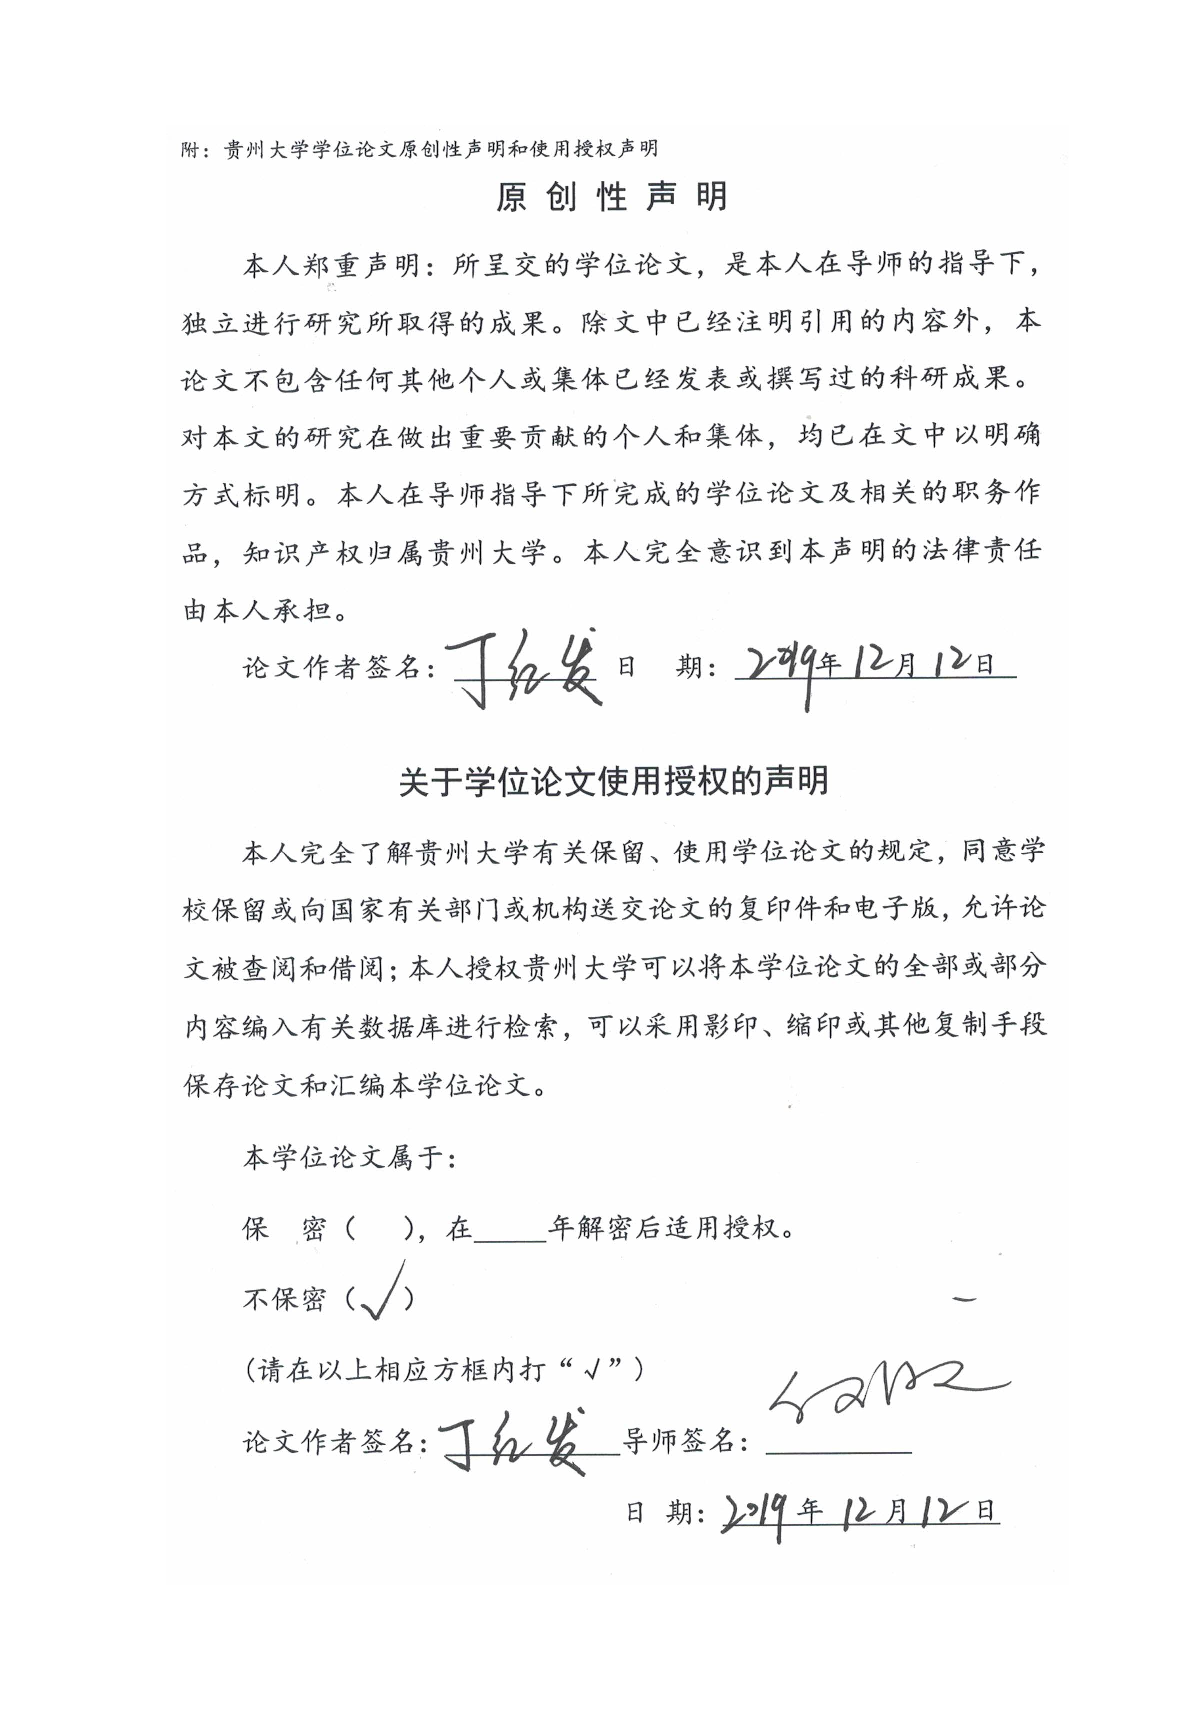
\includegraphics[width=\textwidth]{shengming2.pdf}
\end{figure}
\end{center}


\end{document}
